% SPDX-FileCopyrightText: 2023 SAP SE
%
% SPDX-License-Identifier: Apache-2.0
%
% This file is part of FEDEM - https://openfedem.org

%%%%%%%%%%%%%%%%%%%%%%%%%%%%%%%%%%%%%%%%%%%%%%%%%%%%%%%%%%%%%%%%%%%%%%%%%%%%%%%%
%
% FEDEM User Guide.
%
%%%%%%%%%%%%%%%%%%%%%%%%%%%%%%%%%%%%%%%%%%%%%%%%%%%%%%%%%%%%%%%%%%%%%%%%%%%%%%%%

\documentclass[10pt]{book}

\def\FedemVer{Fedem~8.0}
\def\FedemTG{\FedemVer~User Guide}
\def\FedemTGuide#1{\FedemVer~Theory Guide, {\sl#1}}
\def\ReferenceImg{../ReferenceGuide/img}

\setlength{\paperwidth}{7.5in}
\setlength{\paperheight}{9.0in}
\setlength{\oddsidemargin}{1.25in}  % 1.0+1.0 = 2.25in
\setlength{\evensidemargin}{0.75in} % 1.0+0.0 = 1.75in
\setlength{\topmargin}{-0.5in}      % 1.0-0.5 = 0.5in
\setlength{\headheight}{0.5in}
\setlength{\headsep}{0.275in}
\setlength{\textwidth}{4.75in}
\setlength{\marginparwidth}{1.0in}
\setlength{\marginparsep}{0.25in}
\setlength{\footskip}{0.5in}

\setlength{\textheight}{\paperheight}
\addtolength{\textheight}{-1.0in}
\addtolength{\textheight}{-\topmargin}
\addtolength{\textheight}{-\headheight}
\addtolength{\textheight}{-\headsep}
\addtolength{\textheight}{-\footskip}
\addtolength{\textheight}{-0.35in} % Desired space at bottom of page

\setlength{\itemsep}{0pt}
\setlength{\topsep}{0pt}
\setlength{\parsep}{\parskip}

\usepackage{parskip}
\usepackage{graphpap}
\usepackage{amsmath,amssymb}
\usepackage{amstext}
\usepackage{graphicx}
\usepackage{tikz}

\usepackage{wrapfig}
\usepackage{colortbl}
\usepackage{float}
\usepackage{threeparttable}
\usepackage{tabto}

\usepackage[backref]{hyperref}
\hypersetup{colorlinks=true,linkcolor=blue,urlcolor=blue}
\hypersetup{pdftitle=\FedemTG,pdfauthor=Knut Morten Okstad - SAP SE}
\hypersetup{pdfsubject=User Guide for the FEDEM Simulation Software}
\hypersetup{pdfkeywords=FEM Model reduction Multi-body dynamics}
\usepackage{../sty/chappg} % Set up page numbering with chapter and page number
\usepackage{../sty/my_sections}
\usepackage{../sty/my_headings}
\usepackage{../sty/my_chapter}
% SPDX-FileCopyrightText: 2023 SAP SE
%
% SPDX-License-Identifier: Apache-2.0
%
% This file is part of FEDEM - https://openfedem.org

\newcommand{\namelistlabel}[1]{\mbox{#1}\hfil}
\newenvironment{namelist}[1]
{
  \begin{list}{}
  {
    \let\makelabel\namelistlabel
    \settowidth{\labelwidth}{#1}
    \setlength{\leftmargin}{\labelwidth}
    \addtolength{\leftmargin}{\parindent}
    \addtolength{\leftmargin}{\labelsep}
    \setlength{\itemsep}{0pt}
    \setlength{\topsep}{0pt}
    \setlength{\parsep}{\parskip}
  }
}
{
  \end{list}
}

\newcounter{myEnumC1}
\renewenvironment{enumerate}
{
  \begin{list}{\arabic{myEnumC1}.}
  {
    \usecounter{myEnumC1}
    \setlength{\itemsep}{0pt}
    \setlength{\topsep}{0pt}
    \setlength{\parsep}{\parskip}
  }
}
{
  \end{list}
}

\renewenvironment{itemize}
{
  \begin{list}{\labelitemi}
  {
    \usecounter{myEnumC1}
    \setlength{\itemsep}{0pt}
    \setlength{\topsep}{0pt}
    \setlength{\parsep}{\parskip}
  }
}
{
  \end{list}
}

% SPDX-FileCopyrightText: 2023 SAP SE
%
% SPDX-License-Identifier: Apache-2.0
%
% This file is part of FEDEM - https://openfedem.org

% Some useful macros for generating the Fedem Users Guide

\def\IconText#1#2{
 \hskip-25mm
 \begin{minipage}{1.1\textwidth}
  \begin{tabular}{p{0.1\textwidth} p{0.9\textwidth}}
   \includegraphics[width=7mm]{Figures/Icons/#1} &
   \raggedright\vskip-7mm #2
  \end{tabular}
 \end{minipage}}

% Use this instead of \IconText when first paragraph in a section
\def\IconTextFirst#1#2{
 \vskip\parskip
 \hskip\parindent
 \IconText{#1}{#2}}

\def\IconsText#1#2#3{
 \hskip-28.4mm
 \begin{minipage}{1.15\textwidth}
  \begin{tabular}{p{0.03\textwidth} p{0.1\textwidth} p{0.85\textwidth}}
   \includegraphics[width=7mm]{Figures/Icons/#1} &
   \includegraphics[width=7mm]{Figures/Icons/#2} &
   \raggedright\vskip-7mm #3
  \end{tabular}
 \end{minipage}}

\def\IconTextFigure#1#2#3{
 \hskip-20mm
 \begin{minipage}{1.1\textwidth}
  \begin{tabular}{p{0.1\textwidth} p{0.63\textwidth} p{0.25\textwidth}}
   \includegraphics[width=7mm]{Figures/Icons/#1} &
   \raggedright\vspace{-7mm} #2 &
   \vspace{-7mm}\includegraphics[width=0.25\textwidth]{#3}
  \end{tabular}
 \end{minipage}}

\def\GenericNote#1#2#3{
 \hskip-25mm
 \begin{minipage}{1.1\textwidth}
  \begin{tabular}{p{0.1\textwidth} p{0.9\textwidth}}
   \includegraphics[width=8mm]{Figures/#1} &
   \raggedright\vskip-7mm\sl\textbf{#2}: #3
  \end{tabular}
 \end{minipage}}

\def\GenericEnumNote#1#2#3{
 \hskip-28.8mm
 \begin{minipage}{1.1\textwidth}
  \begin{tabular}{p{0.17\textwidth} p{0.83\textwidth}}
   \includegraphics[width=8mm]{Figures/#1} &
   \raggedright\vskip-7mm\sl\textbf{#2}: #3
  \end{tabular}
 \end{minipage}}

% Even more generic, for use within minipages of various size
\def\MiniGenericNote#1#2#3#4#5#6#7{
 \hspace*{#3}
 \begin{minipage}{#4\textwidth}
  \begin{tabular}{p{#5\textwidth} p{#6\textwidth}}
   \includegraphics[width=8mm]{Figures/#1} &
   \raggedright\vskip-7mm\sl\textbf{#2}: #7
  \end{tabular}
 \end{minipage}}

\def\Tip#1{\GenericNote{tip}{TIP}{#1}}
\def\Note#1{\GenericNote{note}{NOTE}{#1}}
\def\Warning#1{\GenericNote{warning}{WARNING}{#1}}
\def\Important#1{\GenericNote{warning}{IMPORTANT}{#1}}
\def\Caution#1{\GenericNote{caution}{CAUTION}{#1}}
\def\EnumTip#1{\GenericEnumNote{tip}{TIP}{#1}}
\def\EnumNote#1{\GenericEnumNote{note}{NOTE}{#1}}
\def\EnumWarning#1{\GenericEnumNote{warning}{WARNING}{#1}}
\def\EnumCaution#1{\GenericEnumNote{caution}{CAUTION}{#1}}

\def\Chapter#1#2{\hypertarget{#2}{\chapter{#1}\label{#2}}}
\def\Section#1#2{\hypertarget{#2}{\section{#1}\label{#2}}}
\def\SubSection#1#2{\hypertarget{#2}{\subsection{#1}\label{#2}}}
\def\SubSubSection#1#2{\hypertarget{#2}{\subsubsection{#1}\label{#2}}}

\def\refAppendix#1#2{\protect\hyperlink{#1}{\sl Appendix~\ref{#1}, ''#2''}}
\def\refChapter#1#2{\protect\hyperlink{#1}{\sl Chapter~\ref{#1}, ''#2''}}
\def\refSection#1#2{\protect\hyperlink{#1}{\sl Section~\ref{#1}, ''#2''}}
\def\refSubSection#1#2#3{\protect\hyperlink{#1}{\sl"#2"} in
                         \protect\hyperlink{#3}{\sl Section~\ref{#3}}}

\def\Registered{\textsuperscript{\textregistered}}

\def\File#1{{\tt#1}}

\def\Bullet#1{
 \begin{picture}(10,10)
  \put(5,5){\circle*{10}}
  \put(2,2){\color{white}\tt#1}
 \end{picture}}
% Use this instead for double-digit bullets
\def\BBullet#1{
 \begin{picture}(10,10)
  \put(5,5){\circle*{10}}
  \put(1,3){\color{white}\tt\footnotesize#1}
 \end{picture}}

% Define environment bulletlist which uses bullets on the item numbers
%---------------------------------------------------------------------
\newcommand*\circled[1]{%
 \tikz[baseline=(C.base)]
 \node[fill=black,draw,circle,inner sep=1.2pt,line width=0.2mm,](C){
  \color{white}\tt#1};}

\newenvironment{bulletlist}{
 \let\olditem\item
 \renewcommand\item[1][]{
  \stepcounter{enumi}
  \olditem[\circled{\theenumi}]##1}
 \renewcommand\subitem{\olditem[--]}
 \begin{enumerate}
 \setcounter{enumi}{0}}{
 \end{enumerate}}
%---------------------------------------------------------------------


\renewcommand{\bottomfraction}{1.0}

%\includeonly{title_and_contents}
%\includeonly{introduction,learning_basics}
%\includeonly{mechanism_modeling}
%\includeonly{mechanism_elements}
%\includeonly{control_system_modeling}
%\includeonly{mechanism_analysis}
%\includeonly{postprocessing_results}
%\includeonly{managing_results}

%\includeonly{fe_model_interface}
%\includeonly{file_types_usage}
%\includeonly{cmd_line_options}
%\includeonly{beta_feature_doc}

\begin{document}
% SPDX-FileCopyrightText: 2023 SAP SE
%
% SPDX-License-Identifier: Apache-2.0
%
% This file is part of FEDEM - https://openfedem.org

%%%%%%%%%%%%%%%%%%%%%%%%%%%%%%%%%%%%%%%%%%%%%%%%%%%%%%%%%%%%%%%%%%%%%%%%%%%%%%%%
%
% FEDEM Theory Guide.
%
%%%%%%%%%%%%%%%%%%%%%%%%%%%%%%%%%%%%%%%%%%%%%%%%%%%%%%%%%%%%%%%%%%%%%%%%%%%%%%%%

\iftoggle{publicedition}{
  \thispagestyle{empty}
  \vspace*{5\baselineskip}
  \begin{minipage}{0.8\textwidth}
    
\includegraphics[width=\textwidth]{../img/Fedem} \\[1cm]
    {\huge\bf Theory Guide} \\[2mm]
    \bf\FedemVer
  \end{minipage}
}{\maketitle}
\pagenumbering{roman}
\renewcommand{\contentsname}{Table of Contents}
\tableofcontents
\listoffigures
\listoftables

\setlength{\parskip}{0.35em}
\pagenumbering{arabic}
\raggedright
%% SPDX-FileCopyrightText: 2023 SAP SE
%
% SPDX-License-Identifier: Apache-2.0
%
% This file is part of FEDEM - https://openfedem.org

\chapter*{Nomenclature}
%
%%%%%%%%%%%%%%%%%%%%%%%%%%%%%%%%%%%%%%
% Small macro for nomenclature items %
%%%%%%%%%%%%%%%%%%%%%%%%%%%%%%%%%%%%%%
%
\newcommand{\nomitem}[2]
{
\item[{\makebox[30mm][l]{#1 \hfill:}}] #2
}
%%%%%%%%%%%%%%%%%%%%%%%%%%%%%%%%%%%%%%
% 
\subsubsection*{Position and Orientation}
\begin{namelist}{{\makebox[30mm][l]{$G = [G_{1} G_{2} G_{3}]$\hfill:}}}
\nomitem{${\mf s} = [s_{x} s_{y} s_{z}]^T$}{Position vector}
\nomitem{${\mf a} = [a_{1} a_{2} a_{3}]^T$}{Position vector}
\nomitem{${\mf p} = [p_{1} p_{2} p_{3}]^T$}{Position vector}
\nomitem{${\mf p} = [p_{x} p_{y} p_{z}]^T$}{Position of supernodes}
\nomitem{${\tf \theta} = [\theta_{x} \theta_{y} \theta_{z}]$}{Rotation vector. 
Rotation angles about $x$, $y$ and $z$-axis. Deformation vector caused by rotations}
\nomitem{$\tf \omega = [\omega_{x} \omega_{y} \omega_{z}]^T$}{Rotational velocity vector. Instantaneous rotation axis.}
\nomitem{$\omega$}{Rotational velocity vector}
%bh\nomitem{$\omega_{c}$}{Some kind of frequency with respect to Control system}
%bh\nomitem{$\omega_{0}$}{Some kind of frequency with respect to Control system}
\end{namelist}
%
\subsubsection*{Displacement}
\begin{namelist}{{\makebox[30mm][l]{$G = [G_{1} G_{2} G_{3}]$\hfill:}}}
\nomitem{${\mf v} = [v_{x} v_{y} v_{z}]^T$}{Displacement vector}
\nomitem{${\mf v}_{r}$}{Rigid body displacement}
\nomitem{${\mf v}_{d}$}{Deformational displacement}
\end{namelist}
%
\subsubsection*{Velocity}
\begin{namelist}{{\makebox[30mm][l]{$G = [G_{1} G_{2} G_{3}]$\hfill:}}}
\nomitem{${\mf\dot v}$}{Velocity vector}
\nomitem{${\mf\dot r}$}{Velocity vector}
\nomitem{${\mf\dot u} = [\dot u \dot v \dot w]$}{Rigid body translational velocity vector}
\nomitem{${\mf\dot v}_{r}$}{Rigid body velocity vector}
\nomitem{${\mf\dot v}_{d}$}{Deformational velocity vector}
\nomitem{${\mf v}_{t}$}{Translational velocity vector}
\nomitem{${\mf v}_{r}$}{Rotational velocity vector}
\nomitem{$v_{D}$}{Damper velocity}
\nomitem{${\mf v} = [\dot x \dot y \dot z]^T$}{Velocity}
\end{namelist}
%
%\subsection*{Eigen problem}
%\begin{namelist}{{\makebox[30mm][l]{$G = [G_{1} G_{2} G_{3}]$\hfill:}}}
%\nomitem{$v_{\lambda}$}{Eigenvector}
%\nomitem{$u_{\lambda}$}{Eigenvector}
%\nomitem{$u$}{Input vector � Control system}
%\end{namelist}
%
\subsubsection*{Acceleration}
\begin{namelist}{{\makebox[30mm][l]{$G = [G_{1} G_{2} G_{3}]$\hfill:}}}
\nomitem{$\mf\ddot v$}{Acceleration vector}
\nomitem{$\mf\ddot r$}{Acceleration vector}
\nomitem{${\mf U}_{x} {\mf U}_{y} {\mf U}_{z}$}
{Force vectors from unit gravitational acceleration in $x$-, $y$-, and $z$-direction}
\end{namelist}
%
\subsubsection*{Latin Symbols}
\begin{namelist}{{\makebox[30mm][l]{$G = [G_{1} G_{2} G_{3}]$\hfill:}}}
\nomitem{$A$}{Incidence matrix. Matrix in eigenvalue problem equation. Runge-Kutta matrix �
Butcher tableau}
\nomitem{$a_{g}$}{Gravitational acceleration}
\nomitem{$a_{t}$}{Translational acceleration vector}
\nomitem{$a_{r}$}{Rotational acceleration vector}
\nomitem{$a_{ij}$}{Runge-Kutta coefficient � control system}
\nomitem{$B$}{Strain-displacement matrix. Strain interpolation matrix. Matrix in eigenvalue
problem equation}
\nomitem{$b$}{Runge-Kutta matrix � Butcher tableau}
\nomitem{$b_{j}$}{Runge-Kutta coefficient � control system}
\nomitem{$C$}{Damping matrix}
\nomitem{$c$}{Reduced damping matrix? Runge-Kutta matrix � Butcher tableau}
\nomitem{$C$}{Constitutive matrix}
\nomitem{$c_{j}$}{Runge-Kutta coefficient � control system}
\nomitem{$E$}{? Matrix in eigenvalue problem equation}
\nomitem{$e_{i}$}{Eccentricity vectors}
\nomitem{$e_{ij}$}{Unit direction vector}
\nomitem{$F^{I}$}{Inertia forces}
\nomitem{$F^{D}$}{Damping forces}
\nomitem{$F^{S}$}{Elastic forces}
\nomitem{$f$}{Force vector}
\nomitem{$G_{x} G_{y} G_{z}$}{Gravitational force vectors}
\nomitem{$g_{x} g_{y} g_{z}$}{Reduced gravitational force vectors}
\nomitem{$g$}{Superelement gravitational forces}
\nomitem{$G = [G_{1} G_{2} G_ {3}]$}{The G matrix}
\nomitem{$H(\theta)$}{Rodriguez parametrisation}
\nomitem{$H$}{Transformation matrix (model reduction)}
\nomitem{$h$}{Time increment}
\nomitem{$I$}{Mass property matrix (what is this?). Inertia matrix}
\nomitem{$I_{G}$}{?}
\nomitem{$I$}{Identity matrix}
\nomitem{$i_{1}, i_{2}, i_{3}$}{Orthonormal base vectors in local coordinate system}
\nomitem{$I_{1}, I_{2}, I_{3}$}{Orthonormal base vectors in global coordinate system}
\nomitem{$K$}{Stiffness matrix}
\nomitem{$k$}{Reduced stiffness matrix?}
\nomitem{$k_{G}$}{Rotational geometric stiffness matrix}
\nomitem{$k_{M}$}{Material stiffness matrix}
\nomitem{$k_{e}$}{Linear stiffness matrix}
\nomitem{$L$}{Angular momentum? Spin?}
\nomitem{$M$}{Mass matrix}
\nomitem{$M_{r}$}{Reduced mass matrix}
\nomitem{$m$}{No name in manual (reduced mass matrix??). transformed mass matrix. reduced superelement
mass matrix. element mass matrix}
\nomitem{$m_{1} m_{2} m_{3}$}{Some kind of position matrices ??}
\nomitem{$m_{1} \, etc \, m_{N}$}{Torque?} 
\nomitem{$m$}{Lumped mass}
\nomitem{$N$}{Newton matrix}
\nomitem{$n$}{Reduced superelement Newton matrix}
\nomitem{$n_{1} \, etc \, n_{N}$}{Force?}
\nomitem{$n_{a}$}{???}
\nomitem{$P$}{Position and orientation matrix}
\nomitem{$p = [p_{x}, p_{y}, p_{z}]$}{Position (of supernodes)}
\nomitem{$Q$}{External load vector / external force vector / input load} 
\nomitem{$q$}{No name in manual (reduced external load vector ??) Generalized DOFs. 
              Reduced set of displacements. What is the difference between q and y??}
\nomitem{$R$}{Orientation matrix. Rotation matrix}
\nomitem{$R_{a}$}{Rigid body displacement vector}
\nomitem{$S$}{Stiffness force. What is this compared to F S ?}
\nomitem{$s$}{Laplace variable ? � control system}
\nomitem{$t$}{Torque vector}
\nomitem{$T$}{Transformation matrix from local to global coordinate system}
\nomitem{$T_{n}$}{Transformation matrix from local to global coordinate system}
\nomitem{$T_{{\varepsilon}_{r}}$}{??}
\nomitem{$T$}{Period}
\nomitem{$t_{k}$}{time at k}
\nomitem{$U_{e}$}{Strain energy}
\nomitem{$U_{k}$}{Kinetic energy}
\nomitem{$U_{p}$}{Potential energy}
\nomitem{$U_{i}$}{Input energy}
\nomitem{$U_{d}$}{Energy loss}
\nomitem{$U_{sum}$}{Energy check-sum}
\nomitem{$x$}{State variables � control system}
\nomitem{$y$}{Generalized DOFs (vibration modes)}
\nomitem{$z$}{Algebraic variables � control system}
\end{namelist}
%
\subsubsection*{Greek Symbols}
\begin{namelist}{{\makebox[30mm][l]{$G = [G_{1} G_{2} G_{3}]$\hfill:}}}
\nomitem{$\gamma$}{Newmark integration parameter}
\nomitem{$\beta$}{Newmark integration parameter. Reighleigh damping coefficient}
\nomitem{$\alpha$}{Newmark numerical damping factor. Reighleigh damping coefficient}
\nomitem{$\alpha_{1}$}{Mass proportional damping coefficient (structural damping)}
\nomitem{$\alpha_{2}$}{Stiffness proportional damping coefficient (structural damping)}
\nomitem{$\mu$}{Shift value (Eigenvalue problem}
\nomitem{$\lambda$}{Structural damping ratio}
\nomitem{${\tf \lambda}_{u}$}{Eigenvalue � undamped system}
\nomitem{${\tf \lambda}_{d}$}{Eigenvalue � damped system}
\nomitem{$\varepsilon$}{Tolerance}
\nomitem{$\tf \varepsilon$}{Strain vector}
\nomitem{$\tf \sigma$}{Stress vector}
\nomitem{$\tf \phi$}{Eigenvector}
\nomitem{$\tf \Phi$}{Eigenvector matrix}
\end{namelist}
%
\subsubsection*{Subscripts}
\begin{namelist}{{\makebox[30mm][l]{$G = [G_{1} G_{2} G_{3}]$\hfill:}}}
\nomitem{$CG$}{Centre of Gravity}
\nomitem{$RB$}{Rigid Body}
\nomitem{$CR$}{Centre of Rotation}
\end{namelist}
%
\subsubsection*{Superscripts}
\begin{namelist}{{\makebox[30mm][l]{$G = [G_{1} G_{2} G_{3}]$\hfill:}}}
\nomitem{${\tilde{\;}}$}{The parameter is given in a local coordinate system}
\nomitem{${\hat{\;}}$}{Spin of a matrix}
\nomitem{${\overline{\;}}$}{Transformed parameter}
\nomitem{${\dot{\;}}$}{Time derivative}
\end{namelist}
% SPDX-FileCopyrightText: 2023 SAP SE
%
% SPDX-License-Identifier: Apache-2.0
%
% This file is part of FEDEM - https://openfedem.org

%%%%%%%%%%%%%%%%%%%%%%%%%%%%%%%%%%%%%%%%%%%%%%%%%%%%%%%%%%%%%%%%%%%%%%%%%%%%%%%%
%
% FEDEM Theory Guide.
%
%%%%%%%%%%%%%%%%%%%%%%%%%%%%%%%%%%%%%%%%%%%%%%%%%%%%%%%%%%%%%%%%%%%%%%%%%%%%%%%%

\chapter{Introduction}

\pagenumbering{arabic}

Fedem, an abbreviation for Finite Element Dynamics in Elastic Mechanisms,
is a code for effective modeling, simulation and visualization of finite element
assemblies and control systems. The code is based on a non-linear finite element
formulation, which predicts the dynamic response of elastic mechanisms
experiencing non-linear effects such as large rigid-body rotations.
The elastic and rigid-body motions of a mechanism are solved together
with control systems. Fedem represents in this respect
\textit{Multidisciplinary Mechanical Analysis}.

This theory guide is intended to provide users and others with insight into
the mathematical and physical basis of the numerical simulation code.

% SPDX-FileCopyrightText: 2023 SAP SE
%
% SPDX-License-Identifier: Apache-2.0
%
% This file is part of FEDEM - https://openfedem.org

%%%%%%%%%%%%%%%%%%%%%%%%%%%%%%%%%%%%%%%%%%%%%%%%%%%%%%%%%%%%%%%%%%%%%%%%%%%%%%%%
%
% FEDEM Theory Guide.
%
%%%%%%%%%%%%%%%%%%%%%%%%%%%%%%%%%%%%%%%%%%%%%%%%%%%%%%%%%%%%%%%%%%%%%%%%%%%%%%%%

\section{History}

The theory behind Fedem was originally developed by professor Ole Ivar Sivertsen
in the late 1970s and through the 1920s. His work initiated new Ph.D.\ studies
and international R\&D projects that contributed to the development of the first
FEDEM software product.

On the basis of Professor Sivertsen's work, a company was established in 1992
by Sintef, Northern Europe's largest R\&D institute based in Trondheim.
Computer speed reached levels that would allow the theories to produce results,
and visualization technology made it possible to create a user interface.
During this period the Fedem software was strictly an inhouse code at Sintef.

In 1995 the company Fedem, which later became Fedem Technology,
continued the development of the user interface and made it possible to offer
Fedem as a commercial product in 1998.

The Fedem software was continously developed as a product by Fedem Technology
during the 2000s and 2010s while it was also used as an internal tool in
various consultancy projects, until the company was aquired by SAP SE in 2016.
Since then, the Fedem solvers have been provided as components in the
EPD Connected Products by SAP, until the sunsetting of the Connected Products
in 2023. It was then decided to release Fedem under a open source license
on github, as a service to the existing user community.


\section{System Simulation Methods}

One method of System Simulation is the so-called Multi Body System Simulation, with which 
the real physical behavior of the product under investigation can be reduced 
to a few - for instance overall behavior relevant - characteristics and then 
can be simulated as a numerical model on the computer. Each body is usually
treated as completely rigid.

The Finite Element Method is used for instance 
for a vehicle to calculate fatigue, stiffness, dynamical behavior of the car 
body, of chassis components, of engines.  
The size and the shape of the Finite Elements are chosen according to the
required accuracy of the results. For many years the Finite Element Method has 
been a successful tool for product analysis with respect to 
functionality and safety.

New simulation tools are now commercially available, the so-called 
Multi Discipline Simulation tools, which combine Multi Body System 
Simulation, the Finite Element Method and Control Engineering. These 
computer programs make a much more detailed modeling possible and 
correspondingly yield much more accurate Multi Body System Simulation results.

\section{Terminology and Definitions}

Most of the terms and names used within Fedem is quite standard within Finite Element technology
and dynamic simulation. However, over the years certain terms have evolved among users and
developers of the software, to a point where the terminology has become an integral part of
the software product. 

\begin{itemize}

\item[\bf DOF]
Degree of Freedom. For the mechanism models of Fedem, a DOF is usually a translational
or rotational degree of freedom. Regarding a control system a DOF is defined more broadly as
simply an unknown of the equation system to be solved.

\item[\bf Triad]
Numerically a triad is simply a node with displacement DOFs. The term has
been coined within the modeling frame to better to describe the modeling entity that eventually
results in a node in the computational model. Because of its frequent use within the modeling
vocabulary it has also come to be used synonymously with nodes within the numerical/theoretical
vocabulary of Fedem.

\item[\bf Link]
Regarding numerical algorithms a link is a superelement. The element is linear within
its corotated coordinate system. This term also has its background from the modeling
side of Fedem and has since become a part of the theoretical vocabulary.

\item[\bf Model]
A model is defined as a more or less simplified representation 
of a system. The model must represent the properties of a system being studied,
as accurate as possible.

\item[\bf Simulation]
Imitation of certain properties of a (mechanical) system in a computational model.

\item[\bf Kinematic simulation]
Kinematic simulation refers to calculations of motion in a system 
with no reference to forces and torques necessary to achieve this motion.

\item[\bf Dynamic simulation]
Dynamic simulation refers to the calculations of motion in a system 
where both constraint forces and forces necessary to drive the system are 
taken into account.

\item[\bf Multi discipline dynamic simulation]
The multi discipline dynamic simulation concept refers to a 
simulation model where the overall system is modeled as a mechanism, the 
parts are modeled as Finite Element substructures, and combined with a 
possible control system, all is integrated in the same simulation model.
A control system may include controllers, actuators and sensors (to model feedback loops).

\item[\bf System simulation]
The term system simulation incorporates the three terms 
\textit{kinematic simulation}, \textit{dynamic simulation} and 
\textit{multi discipline dynamic simulation} described above.
\end{itemize}

% SPDX-FileCopyrightText: 2023 SAP SE
%
% SPDX-License-Identifier: Apache-2.0
%
% This file is part of FEDEM - https://openfedem.org

%%%%%%%%%%%%%%%%%%%%%%%%%%%%%%%%%%%%%%%%%%%%%%%%%%%%%%%%%%%%%%%%%%%%%%%%%%%%%%%%
%
% FEDEM User Guide.
%
%%%%%%%%%%%%%%%%%%%%%%%%%%%%%%%%%%%%%%%%%%%%%%%%%%%%%%%%%%%%%%%%%%%%%%%%%%%%%%%%

\def\Variable#1{\textless#1\textgreater}
\def\Untitled{\File{untitled\_\Variable{\#}.fmm}}


\Chapter{Learning the Basics}{learning-the-basics}

This chapter outlines some system requirements,
explains how and where models and their results are saved,
and introduces the Fedem GUI with some basic commands.

Sections in this chapter address the following topics:

\begin{itemize}
\item
  \protect\hyperlink{system-requirements}
                    {System requirements}
\item
  \protect\hyperlink{storing-models-and-results}
                    {Storing models and results}
\item
  \protect\hyperlink{starting-fedem}
                    {Starting Fedem}
\item
  \protect\hyperlink{touring-the-interface}
                    {Touring the interface}
\item
  \protect\hyperlink{executing-commands}
                    {Executing commands}
\item
  \protect\hyperlink{visualizing-the-model}
                    {Visualizing the model}
\item
  \protect\hyperlink{opening-and-saving-model-files}
                    {Opening and saving model files}
\item
  \protect\hyperlink{loading-and-unloading-fe-data}
                    {Loading and unloading FE-Data}
\item
  \protect\hyperlink{exporting-objects}
                    {Exporting objects}
\item
  \protect\hyperlink{customizing-fedem-using-plug-ins}
                    {Customizing Fedem using plug-ins}
\item
  \protect\hyperlink{customizing-fedem-using-addons}
                    {Customizing Fedem using Addons}
\end{itemize}

\clearpage


%%%%%%%%%%%%%%%%%%%%%%%%%%%%%%%%%%%%%%%%%%%%%%%%%%%%%%%%%%%%%%%%%%%%%%%%%%%%%%%%
\Section{System requirements}{system-requirements}

The following are minimum system/hardware requirements and recommended
settings for optimal Fedem performance.

\Note{Use of resolution settings other than those recommended below may
  require you to move or resize windows and dialog boxes to fit your screen.}

\begin{center}
\begin{threeparttable}[b]
\begin{tabular}{ | m{3.5cm} | m{6.5cm} | }
    \hline
    \textbf{Processor}  & Recommended: Pentium 4 @ 2 GHz. \newline
                          Minimum: Pentium III @ 850 MHz. \\ \hline
    \textbf{RAM}  & Recommended: 2 GB. Minimum: 256 MB. \\ \hline
    \textbf{Free disk space} &  Dependent upon the size and complexity of mechanism models.\tnote{1} \\ \hline
    \textbf{Graphics card}   & Recommended: high end graphics card. \newline
                     Required: OpenGL\Registered API support. \\ \hline
    \textbf{Pointing device} &  Three-button mouse with wheel. \\ \hline
    \textbf{Resolution setting} &  1,280 x 1,024 pixels or higher. \\ \hline
\end{tabular}
\begin{tablenotes}
  \item[1]{Larger models may require several GBs.}
\end{tablenotes}
\end{threeparttable}
\end{center}


%%%%%%%%%%%%%%%%%%%%%%%%%%%%%%%%%%%%%%%%%%%%%%%%%%%%%%%%%%%%%%%%%%%%%%%%%%%%%%%%
\Section{Storing models and results}{storing-models-and-results}

Fedem uses the following files and directories to store the contents of a model:

\begin{itemize}
\item The mechanism assembly description and all simulation parameters
  are saved in the Fedem Mechanism Model (\File{.fmm}) format.
  This file is called the model file and contains the complete description
  of your model except for the FE data files and the simulation results.
\item FE data files and all simulation results are saved in a directory named
  \File{\Variable{modelfilename}\_RDB} (the model name specified by the user
  is substituted for \File{\Variable{modelfilename}}).
  Fedem creates this directory in the same location as your model file.
  Within this directory, the FE data files are stored in a directory named
  \File{link\_DB}, unless a FE model repository is used
  (see \refSection{using-fe-model-repositories}{Using FE model repositories}).
\end{itemize}

\refAppendix{file-types-and-usage}{File Types and Usage} contains more
information about Fedem file types, whereas the directory structure is shown in
\refSection{rdb-directory-structure}{RDB directory structure}.


\SubSection{FTL format}{ftl-format}

The Fedem Technology Link (\File{.ftl}) format is used to store
FE models as sets of data in text format
(see \refSection{fedem-technology-link-format}{Fedem Technology Link format}
for more information about the \File{.ftl} file format).


\SubSection{FTC format}{ftc-format}

The Fedem Technology Cad (\File{.ftc}) format may be used to store CAD
geometry in text format.


\SubSection{Other supported formats}{other-supported-formats}

Fedem can import FE models
(see \refSection{creating-parts-by-file-import}{Creating parts by file import})
in the MSC.Nastran Bulk Data File (\File{.bdf} or \File{.nas}) format
(see \refSection{nastran-bulk-data-file-format}{Nastran Bulk Data File format})
and the SESAM input interface file (\File{.FEM}) format.
Earlier versions used the Fedem Link Model (\File{.flm}) format.
This file format is still supported for backward compatibility.

Fedem can also import CAD geometry from VRML files (\File{.wrl}, \File{.vrml},
\File{.vrl}, \File{.wrz}) for visualization of Generic Parts
(see \refSection{parts}{Parts}).


%%%%%%%%%%%%%%%%%%%%%%%%%%%%%%%%%%%%%%%%%%%%%%%%%%%%%%%%%%%%%%%%%%%%%%%%%%%%%%%%
\Section{Starting Fedem}{starting-fedem}

Fedem can be started from either the Windows Start menu,
the Windows file browser, or the command prompt.

\begin{itemize}
\item To start Fedem with a new, empty model, press the Fedem icon on the
  Windows Desktop or choose \textbf{Fedem} from the Windows Start menu.
\item To start Fedem and open an existing model, double-click the icon
  representing the desired model file in the Windows file explorer.
\item Open a command prompt, navigate to the installation directory of Fedem
  and type \File{fedem} optionally followed by some command line options
  (see \refSection{command-line-options}{Command-line options}).
\item To open an existing model from the command prompt,
  navigate to the installation directory and type
  \File{fedem -f \Variable{modelpath}.fmm} substituting
  \File{\Variable{modelpath}} with the path and base name of your model file.
  Alternatively, navigate to the directory of the model file and type
  \File{\Variable{installationdir}/fedem -f \Variable{modelfile}.fmm}, where
  \File{\Variable{installationdir}} is replaced by
  the directory name of the Fedem installation, and
  \File{\Variable{modelfile}} is the base name of the model.
\end{itemize}

When Fedem is started with a new, empty model, the model file is named
\Untitled, where \File{\Variable{\#}} indicates a unique running number. This
empty model file will contain only some default settings, animations and graphs.
The file will be created in your default login directory when Fedem is started
from the Desktop icon or from the Windows Start menu.


\SubSection{Command-line options}{command-line-options}

Fedem has several command-line options that can be used to achieve
different tasks or settings. These options can be invoked when starting
Fedem from the command prompt. Among others, you have options for
starting Fedem in batch mode without any GUI at all, which is useful when
you just want to run an existing model without modifying it.
Refer to \refSection{fedem-gui-options}{Fedem GUI options}
for the complete list of available command-line options.

\Tip{You can create a new model file with a specific name by specifying
  a path and filename that does not yet exist, using the -f option.
  The file will be created for you and opened when Fedem starts.}


\SubSection{Template model file}{template-model-file}

The default settings of a new model are stored in a template model file
which is loaded whenever a new model is created
(either when Fedem is started, or when using the \textbf{New} command,
see \refSection{starting-a-new-model}{Starting a new model"}).
The template file can be modified or changed as needed, and is located in
\File{\Variable{installationdir}/Templates/default.fmm}.

If a different location for the template file is wanted, the environment
variable FEDEM\_TEMPLATE\_FILE can be defined to contain the desired
path to the template file.

\subsubsection{Predefined template files}

The \File{Templates} directory of the Fedem installation contains three
files; \File{default.fmm}, \File{default\_m.fmm} and \File{default\_mm.fmm}.
The files \File{default.fmm} and \File{default\_m.fmm} are identical and
suitable for models using SI unit set, while \File{default\_mm.fmm} contains
default settings that are suitable for models using millimeter, newton and
mega gram as unit set. Simply copy the file \File{default\_mm.fmm} to
\File{default.fmm} if you prefer mm/N/Mg as your default unit set.


\SubSection{Console window}{console-window}

When Fedem is started on a Windows system, a separate console window can
be opened in addition to the Fedem main window, by specifying the
command-line option \File{-console}. This window lists some startup
messages, and may also contain some low-level error messages during a
Fedem session, that normally can be ignored by users, but sometimes
might help understanding an abnormal incident.

\Warning{Once opened, the separate console window must remain open
  throughout the whole Fedem session; closing it explicitly closes the entire
  Fedem session immediately, without the option to save unsaved work.}

\Tip{If abnormal behavior occurs, or if Fedem stops responding,
  check the console window (if activated) and the Output List
  (discussed later) for important information.
  Take note of any errors or warnings before contacting Fedem technical support
  (\href{mailto:support@fedem.com}{\nolinkurl{support@fedem.com}}).}

After finishing some initial setup tasks, the Fedem GUI main window will appear.
In the following sections, the Fedem GUI is described in detail.


%%%%%%%%%%%%%%%%%%%%%%%%%%%%%%%%%%%%%%%%%%%%%%%%%%%%%%%%%%%%%%%%%%%%%%%%%%%%%%%%
\Section{Touring the interface}{touring-the-interface}

\SubSection{Main window}{main-window}

Starting with an empty model file,
the main window of the Fedem GUI appears, as shown below.

\begin{figure}[H]
  \begin{picture}(360,260)
    \put(-80,169){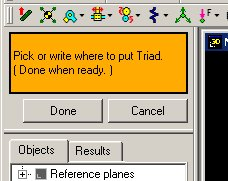
\includegraphics[width=0.2\textwidth]{Figures/2-Guide}}
    \put(15,0){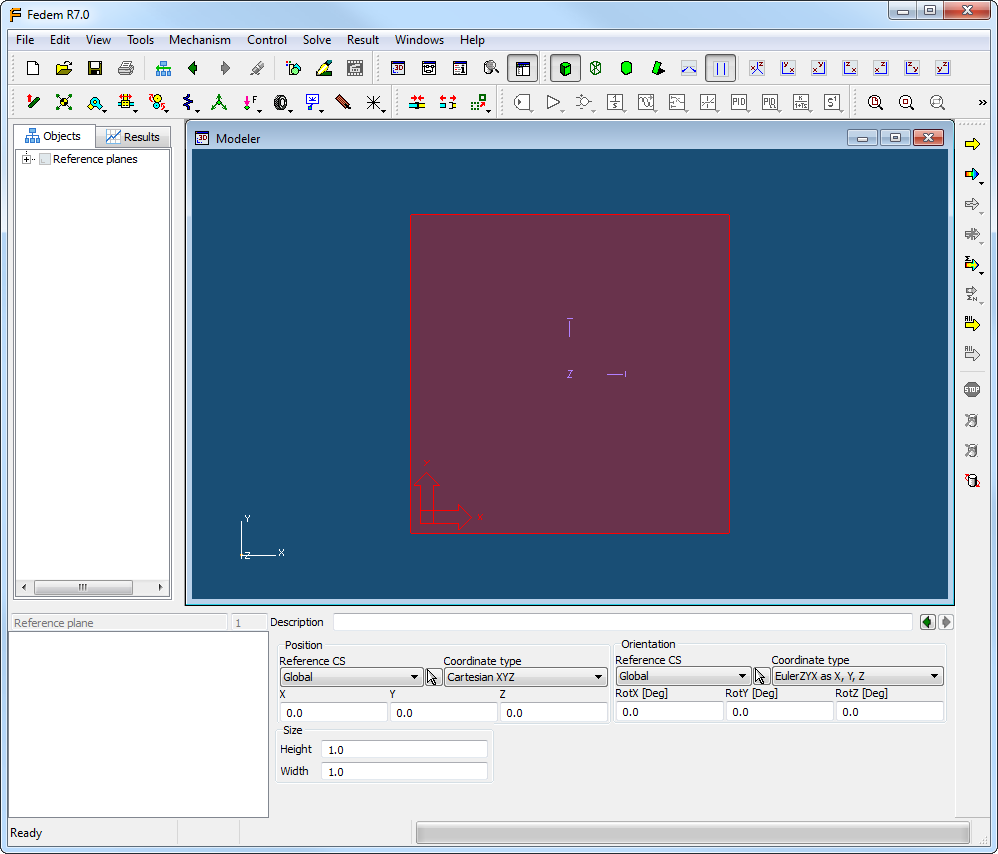
\includegraphics[width=0.85\textwidth]{Figures/2-MainUI}}
    \put(-8,222){\Bullet{1}\huge\{}
    \put(55,205){\Bullet{2}}
    \put(-88,215){\Bullet{3}}
    \put(100,205){\Bullet{4}}
    \put(55,53){\Bullet{5}}
    \put(120,55){\Bullet{6}}
    \put(40,1){\Bullet{7}}
  \end{picture}
\end{figure}

\begin{bulletlist}
\item{\sl Menus and tool bars} --
  contain buttons used to initiate commands.
\item{\sl Model Manager panel} --
  contains the {\sl Objects} and {\sl Results} tabs, which allow you to create,
  manage, and delete the objects in your model and define Animations and Graphs
  of your results.
\item{\sl Guide panel} --
  This orange panel may pop up above the Model Manager panel when you invoke
  a command. It will tell you what you are expected to do during the different
  steps of the command. It also provides \textbf{Done} and \textbf{Cancel}
  buttons used to accept choices or to cancel the command, respectively.
\item{\sl Workspace area} --
  contains the {\sl Modeler}, {\sl Control Editor} and {\sl Graph} views
  for constructing and viewing models and results.
\item{\sl ID and Topology panel} --
  lists objects related to the selected item.
\item{\sl Property Editor panel} --
  allows you to view and edit the properties of individual objects in the model.
\item{\sl Status bar} --
  provides information of the status, progress information
  and whether a solver process is running.
\end{bulletlist}


\SubSection{Menus and tool bars}{menus-and-tool-bars}

Fedem commands are initiated from buttons on the tool bars and menus.
All commands can be accessed from the menus, while the tool bars display only
the most commonly used commands.
The menus are arranged from left to right in logical order of task execution,
starting with standard file functions, then continuing with viewing commands,
mechanism modeling, control system modeling, analysis/solution tools,
and finally results management.


\subsubsection{Command sensitivity}

Menu and tool bar buttons are sensitive to the active view and object
selection. For example, if an object in the {\sl Modeler} view is
selected, the {\sl Graph} view controls appear dimmed (grayed-out) and
cannot be selected.

\subsubsection{Fedem tool bars}

Fedem uses the following tool bars (a tool bar handle to the left (or on
top) marks the beginning of a tool bar):

\begin{itemize}
\item{\sl Standard} --
  provides standard file operations such as \textbf{Open}, \textbf{Save},
  \textbf{Exit}, and selecting and deleting objects.
\item{\sl Windows} --
  provides commands for controlling the active view selection
  ({\sl Modeler}, {\sl Control Editor}, {\sl Output List},
  {\sl Result File Browser})
  and hiding/showing the Model Manager and Property Editor panels.
\item{\sl Zoom and Pan} --
  provides commands for zooming and panning of {\sl Graph} view displays.
  (See \refSection{zoom-and-pan}{Zoom and Pan} for more information
  about these commands.)
\item{\sl 3D View Control} --
  includes commands for rotating the view and changing the view perspective
  in the {\sl Modeler} view. (See \refSection{view-controls}{3D View controls}
  for information about manipulating the view.)
\item{\sl Solvers} --
  these commands are used to set up, start, and stop mechanism analyses,
  and to calculate specific results.
  (See \refChapter{mechanism-analysis}{Mechanism Analysis} for information
  about these commands.)
\item{\sl Mechanism Creation} --
  contains commands for importing parts and creating mechanism entities
  such as Joints, Springs, Dampers, Forces, Sensors, etc.
  (See \refChapter{mechanism-elements}{Mechanism Elements} for more information.)
\item{\sl Mechanism Tools} --
  provides commands used in modeling such as moving, attaching, copying objects,
  and applying motion constraints.
  (See \refChapter{mechanism-elements}{Mechanism Elements}
  for information about modeling tools.)
\item{\sl Control Creation} --
  provides commands for creating control objects.
  (See \refChapter{control-system-modeling}{Control System Modeling}
  for detailed descriptions of control objects.)
\item{\sl Control Tools} --
  contains commands for manipulating the control system.
  (See \refChapter{control-system-modeling}{Control System Modeling}
  for information about modeling control systems.)
\end{itemize}

\SubSubSection{Manipulating tool bars}{manipulating-tool-bars}

\begin{wrapfigure}{r}{0.25\textwidth}
  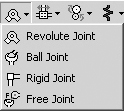
\includegraphics[width=0.25\textwidth]{Figures/1st_Joint_Pulldown}
\end{wrapfigure}

Only some of the commands accessible from the tool bars are displayed. You will
see that there are arrows ($\blacktriangledown$) beside some of the icons.
To access other commands, click and hold down the $\blacktriangledown$ button.
A menu of additional, related commands is displayed (example at right).
Selecting a command from the menu initiates the command and replaces the
button’s function with that of the new command. You can select another
option at any time by clicking, holding down the $\blacktriangledown$ button,
and selecting a different command.

\clearpage
Fedem provides several ways to manage tool bars:

\begin{itemize}
\item Right-click a tool bar handle and select an option
  to relocate, show, or hide the tool bar.
\item Right-click an empty space in the tool bar area and select
  an option from the list to show or hide a tool bar.
\item Double-click a tool bar handle to show or hide the tool bar.
\item Drag a tool bar handle to the left, right, top, or bottom of
  the main window to relocate the tool bar.
\end{itemize}


\SubSection{Model Manager}{model-manager}

\begin{wrapfigure}{r}{0.35\textwidth}
  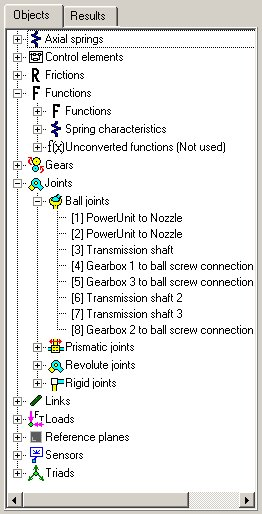
\includegraphics[width=0.35\textwidth]{Figures/2-ModelManager}
\end{wrapfigure}

The Model Manager Panel contains lists of all the objects and result views
that make up your model. This includes mechanism, modeling, and control
system objects, along with animations and graphs. In each list,
objects are grouped by type and sorted by identification numbers or names.
In the Model Manager panel, right-click menus can access several
commands that can be applied to the selected objects.

% Can't use the \Note macro here due to the wrapfigure above
\MiniGenericNote{note}{NOTE}{-25mm}{0.8}{0.13}{0.7}{
  The Objects and Results lists are empty (or nearly empty)
  until you create some items.}

\SubSubSection{Selecting items}{selecting-items}

In the Model Manager panel, you can select items in several ways:
\begin{itemize}
\item Highlight a single item.
\item Hold down the Shift key and click multiple items.
\item Hold down the Ctrl key and click multiple items
  (or a single item to select/deselect).
\item Click and drag the mouse over multiple items.
\end{itemize}

\subsubsection{Deselecting items}

To deselect all items, right-click an empty space in the Model Manager panel.

\subsubsection{Sorting}

The objects in the Model Manager panel can be sorted, either by ID-number or
by item name. To switch sorting mode, right-click inside the panel and
select either Sort by ID or Sort by Name from the menu that appears.
By default, the sorting is based on ID-numbers.

\Tip{Right-clicking in the Model Manager panel will display a pop-up menu
  with commands that applies to the current selection.
  The contents of this menu depend on the type of the selected object.}

\subsubsection{Objects}

The {\sl Objects} tab displays a list of all modeling objects in your
model. Selecting an item from this list highlights it in the
{\sl Modeler-} or {\sl Control Editor} view and displays its
properties in the Property Editor panel.

\subsubsection{Results}

The {\sl Results} tab displays a list of the result views you have
created. The available result views are graphs which contains curves
(individual sets of plotted data), and animations.

Selecting a graph from this list will cause the view containing the
selected graph to pop up, if loaded. Selecting a curve will highlight it
(the curve is rendered red) and raise the graph view in which it resides
as well.

The properties of the different result objects are shown in the
Property Editor panel when they are selected.

See \refChapter{postprocessing-results}{Postprocessing Results}
for more information about graphed and animated results.


\clearpage
\SubSection{ID and Topology panel}{id-and-topology-panel}

\begin{wrapfigure}{r}{0.4\textwidth}
  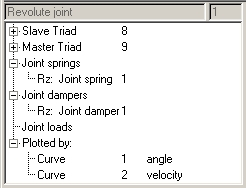
\includegraphics[width=0.4\textwidth]{Figures/ID_Topology window}
  \begin{picture}(135,0)
    \put( 60,105){\Bullet{1}}
    \put(120,105){\Bullet{2}}
    \put(-15, 60){\Bullet{3}}
  \end{picture}
\end{wrapfigure}

When an object in the model is selected, the ID and Topology panel
displays information related to the object as described below.
If multiple items are selected, only the item selected last is displayed.

\begin{bulletlist}
\item{\sl Item Type} --
  the type of the selected object (for example, Revolute joint, Gear, Spring).
\item{\sl ID Number} --
  a unique integer that distinguishes one item of the same type from another.
\item{\sl Topology view} --
  a list that displays the mechanism objects related or connected to
  the selected item.
\end{bulletlist}

\Tip{The Plotted by branch in the Topology view lists all curves that plot
  result quantities from the selected structural object.}

ID numbers are assigned automatically to new objects in numerical order.
If you delete an object such as a Ball joint with ID Number 3, this number
is free and the next Ball joint created is then assigned ID Number 3.

\subsubsection{Topology view and browsing}

Most mechanism components are related to other objects; for example, Joints
consists of Triads that are connected to Parts, and Sensors are measuring
variables from other mechanism components.

These relations are shown by the {\sl Topology} view in a hierarchical fashion,
indicating their topological relationships.
This list can then be used to investigate these related objects,
and to browse through the mechanism model through the topological connections.
This can be done by using the browsing features offered by the
{\sl Topology} view, as described below.

The items in the {\sl Topology} view will be highlighted in the {\sl Modeler}
view when you select an item keeping the mouse button pressed.
This is useful to see exactly which object in the 3D view that corresponds
to the listed item.

\begin{wrapfigure}{r}{0.25\textwidth}
  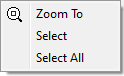
\includegraphics[width=0.25\textwidth]{Figures/2-TopologyViewPopupMenu}
\end{wrapfigure}

Right clicking an item in the {\sl Topology} view will show a tiny pop-up
menu that allows you to either \textbf{Zoom To} or \textbf{Select} the
item, or to do a \textbf{Select All}.

\clearpage
\begin{itemize}
\item\textbf{Zoom To}:
  This command zooms to the item making it easy to locate it in a complex model.
  See also \refSection{zoom-and-pan}{Zoom and Pan}.
\item\textbf{Select}:
  This command selects the right-clicked object from the {\sl Topology} view,
  and thus jump to it showing the properties of that item instead. See also
  \refSection{select}{Select} on how to get back to your previous selection.
\item\textbf{Select All}:
  This command will select all top-level objects currently in the
  {\sl Topology} view, but showing the properties of the last object only.
  The effect of this command is the same as doing a multi-selection from the
  {\sl Objects} list view of Model Manager panel using the \textbf{Shift} key,
  see \refSubSection{selecting-items}{Selecting items}{model-manager}.
\end{itemize}

\Tip{Double clicking an item in the Topology view will also select it.}


\SubSection{Property Editor}{property-editor}

The Property Editor panel is used to view and edit the properties
of mechanism items. The appearance of properties is different
depending on the object selected. The image below is an example
showing properties that are common to some of the Fedem modeling objects.

\begin{figure}[H]
  \begin{picture}(340,75)
    \put( 20, 0){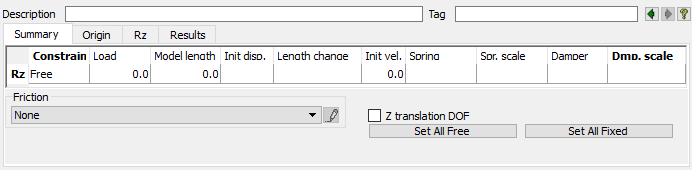
\includegraphics[width=0.9\textwidth]{Figures/2-PropertyPanel}}
    \put( 19, 0){\line(-1,0){7}}
    \put( 12, 0){\line(0,1){65}}
    \put( 12,65){\line(1,0){7}}
    \put( 50,65){\Bullet{1}}
    \put(240,65){\Bullet{2}}
    \put(307,56){\Bullet{3}}
    \put(318,56){\Bullet{4}}
    \put( -2,30){\Bullet{5}}
  \end{picture}
\end{figure}

\begin{bulletlist}
\item{\sl Description} --
  an optional user-supplied name or identifying remarks.
\item{\sl Tag} --
  an optional identifier which can be used to refer to the object from
  python scripts using the fedempy interface.
\item
\includegraphics[scale=0.5]{Figures/Icons/selectbackward}
  
\includegraphics[scale=0.5]{Figures/Icons/selectforward} --
  buttons for navigating back and forth through the latest selections
\item
\includegraphics[scale=2.0]{Figures/icons/help} --
  help button that opens the Reference guide on the Property Editor guide
  content, depending on the type of the selected object.
\item{\sl Properties} --
  editable attributes specific to the selected object.
\end{bulletlist}

\Note{The description field may contain any ASCII-character,
  except for the “-character which is reserved for text string
  delimiters in the model file.}

\Note{The description field is also used to activate beta features,
  see \refAppendix{beta-feature-documentation}{Beta feature documentation}.}

\Caution{After editing a value in the Property Editor panel by typing,
  you must press the Enter key to apply the change.}

\subsubsection{Property menus}

\begin{wrapfigure}{r}{0.4\textwidth}
  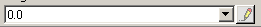
\includegraphics[width=0.4\textwidth]{Figures/2-PropertyValueMenu}
\end{wrapfigure}

Many mechanism items have internal properties that can depend on the
simulation time, measurement of a system variable or some internal
variable in the item in question. Property menus are used to
set up such properties in a simple way. These menus consist of
an option menu that in some cases are editable, and an \textbf{Edit} button.

\begin{wrapfigure}{r}{0.4\textwidth}
  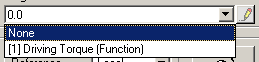
\includegraphics[width=0.4\textwidth]{Figures/2-PropertyValueMenu-Open}
\end{wrapfigure}

The menu contains references to other entities in your model
that can be used as input for the property in question.
A non-linear spring characteristic (e.g., a force-displacement curve)
will be listed in the stiffness property menu of an Axial spring,
Functions and Control outputs will be listed in the magnitude property menu
of a load, etc. Press the menu button to access the list.

\vskip\parskip
\IconText{pencilbutton}{By pressing the \textbf{Edit} button
  you will select the item shown in the menu, as if you had selected it in the
  Model Manager panel.
  This is a convenient way of navigating through the relations of the model,
  giving a simple way of finding the details of a complex model.}

In some of the property menus, a numeric value can be entered
instead of selecting a reference from the menu.
The spring stiffness property is a good example.
Entering a numeric value will assign that value as a constant spring
stiffness to the spring in question.

\Tip{Property menus that accepts a numeric value always have a numeric value
  as default, while “None” is normally the default for Property menus
  not accepting a number.}

To change a property from referring to a constant, select
the top entry in the pull-down list (which is either None
or the last numerical value that was entered in the same box),
or delete the current contents of the box, type in a numerical
value and then press Enter to apply the change.


\clearpage
\SubSection{Object Browser}{object-browser}

An alternative tool to display (but not edit) the detailed properties of
mechanism objects is via the Object Browser dialog box.

\IconText{objectBrowser}{It is opened by selecting \textbf{Objects Browser...}
  from the \textbf{Tools} menu, or from the right-click menu in the
  {\sl Objects} list view of the Model Manager panel.
  The Fedem Object Browser dialog box is shown below.}

\begin{figure}[H]
  \begin{picture}(340,277)
    \put(0,0){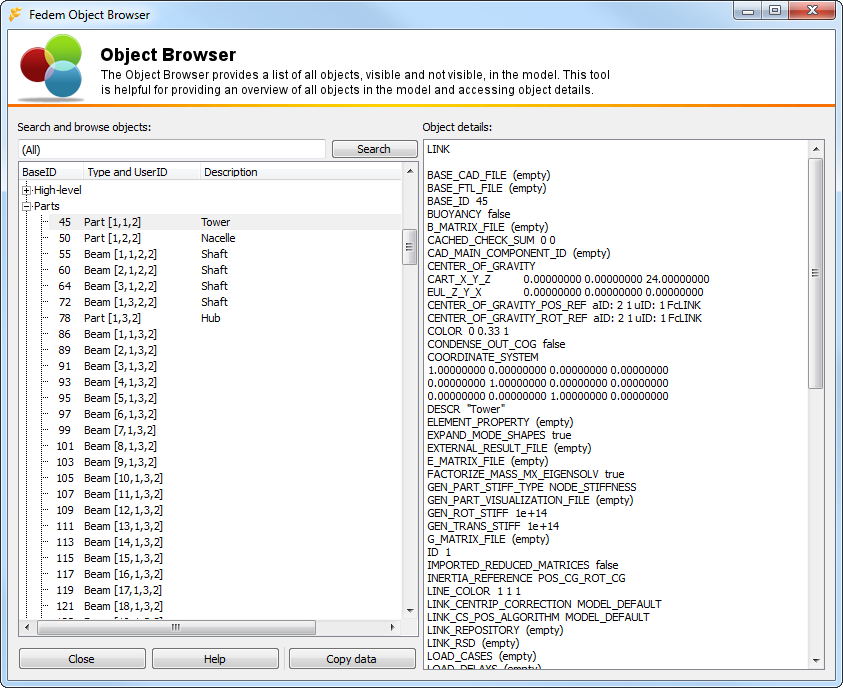
\includegraphics[width=\textwidth]{Figures/Dialogs/2-ObjectBrowser}}
    \put(16,213){\Bullet{1}}
    \put(47,213){\Bullet{2}}
    \put(90,213){\Bullet{3}}
    \put(205,220){\Bullet{4}}
  \end{picture}
\end{figure}

\begin{bulletlist}
\item{\sl BaseID} --
  This column lists the base ID of the objects.
  These are unique ID numbers over all objects in the model that are used for
  internal book-keeping only. They are not visible in the Fedem GUI elsewhere.
\item{\sl Type and UserID} --
  This column lists the type and user ID of the objects, which are used as
  unique identification of the objects elsewhere in the Fedem GUI.
  The user ID consists of a comma-separated list of values in brackets []
  when the object is part of a higher-level sub-assembly, see
  \refSection{user-id-convention}{User ID convention in assemblies}.
\item{\sl Description} --
  This column lists the description string of the objects.
\item{\sl Object details:} --
  This field lists in plain text all the information stored for the selected
  object in the model database. The formatting of this list resembles that of
  the model file (\File{.fmm}) itself.
  The first line contains the model file keyword for the selected object.
  Then the field name (in upper case) and value of each data field of that
  object (including also the base- and user ID and description found in the
  first three column) are listed in alphabetic order of the field name.
\end{bulletlist}

\Tip{The list in the left half of the Object Browser can be sorted with respect
  to the base ID, Type and User ID, or Description, by clicking on the
  respective column headings.}

When opened, the Object Browser dialog box
will display details for the currently selected object in the model. You can
also search for objects by typing their description in the search field and
clicking the search button. The Object Browser will list all objects in the
model if the search field is blank, or if no object was selected when the
dialog box was opened.

\Note{The Object Browser dialog box only displays objects that affect
  the numerical simulation of the model. Therefore, result objects
  (Graphs, Curves, Animations) as well as higher-level sub-assembly objects
  are not listed.}

The main purpose of the Object Browser dialog box is to provide an
overview of the keywords and field names used for the various object types
in the model file, as these are necessary for setting up the simulation events
when, for instance, a model consists of multiple load cases.
See \refSection{using-simulation-events}{Using simulation events}.


\SubSection{Workspace}{workspace}

The Workspace area is used for constructing, manipulating,
and viewing mechanism models, control systems, graphs and animations.
The Workspace can contain several views, including the {\sl Modeler},
{\sl Control Editor}, and multiple {\sl Graph} views.
These views are described in the following sections.

\Tip{The views in the Workspace can be managed using the
  \textbf{Tile} and \textbf{Cascade} commands from the \textbf{Windows} menu.}

\SubSubSection{Modeler}{modeler}

The Modeler view displays a 3D rendering of your mechanism and provides
dynamic viewing capabilities such as zooming, panning, and 2- and 3-dimensional
rotation (see \refSection{navigation}{3D Navigation}).
This view is also used to show animated simulation results.
Select the Modeler view to view, create, or edit a mechanism model.

\IconText{modeler}{To open the Modeler view, select \textbf{Show Modeler}
  from the \textbf{Windows} tool bar or menu.
  The {\sl Modeler} view is then displayed as shown below.
  See also \refSection{modeler-view}{Modeler view}.}

\begin{figure}[!h]
  \center
  \begin{picture}(293,193)
    \put(0,0){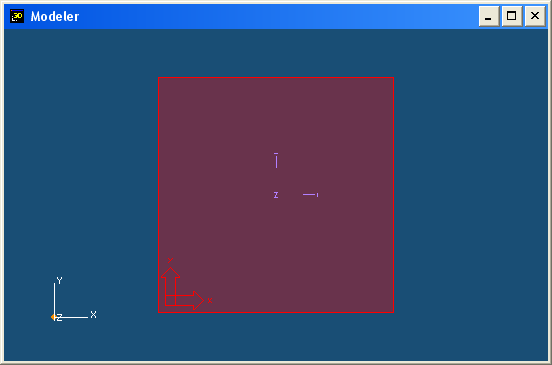
\includegraphics[width=0.85\textwidth]{Figures/2-Modeler}}
    \put(100,100){\Bullet{1}}
    \put(30,30){\Bullet{2}}
  \end{picture}
\end{figure}

\begin{bulletlist}
\item{\sl Reference Plane} --
  The shaded area in the center of the Modeler view represents a plane,
  which can be considered the ground or base for your models.
\item{\sl Global Directions} --
  The arrows located in the lower left corner of the Modeler view show the
  orientation of the global coordinate system and the direction of the
  gravity vector, $\bf g$.
\end{bulletlist}

\Tip{The Modeler view can be expanded to almost full screen size by hiding
  the Model Manager and Property Editor panels. To hide these panels,
  click the \textbf{Model Manager} and \textbf{Property Editor} buttons on
  the \textbf{Windows} tool bar (or from the \textbf{View} menu).
  Hiding the tool bars also increases the viewing area of the {\sl Modeler} view
  (see \refSubSection{manipulating-tool-bars}{Manipulating tool bars}
  {menus-and-tool-bars}).}
\begin{picture}(100,0)
  \put(-77,15){
\includegraphics[width=7mm]{Figures/Icons/modelManager}}
  \put(-49,15){
\includegraphics[width=7mm]{Figures/Icons/propertyPanel}}
\end{picture}

\subsubsection{Control Editor}

The Control Editor view is a workspace for editing the control system.
The graphical representation is a block-based diagram that consists of a series
of control blocks that can be connected to simulate your control system.
This editing environment allows you to create and manipulate the control system
using drag-and-drop functionality. It also features grid and snapping tools
(see \refSection{setting-grid-and-snap}{Setting Grid and Snap}).

\IconText{controlEditor}{To open the Control Editor view,
  click the \textbf{Show Control Editor} button on the \textbf{Windows} tool bar
  (or from the \textbf{Windows} menu). The Control Editor view
  displays the control system (an example is shown below).
  See \refChapter{control-system-modeling}{Control System Modeling}
  for more information on the topic.}

\begin{figure}[H]
  \center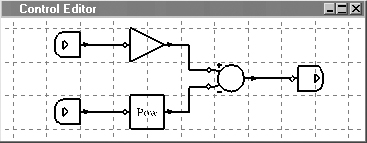
\includegraphics[width=0.8\textwidth]{Figures/cs_example}
\end{figure}

\Note{The Control Editor view is empty until you create control elements.}

\subsubsection{Graph Views}

The Graph view can display various graphed results. You can customize graphs
of selected simulation results and manipulate the Graph view.

\IconText{graphGroup}{To open a Graph view, right-click the Graph from the
  {\sl Results} list of the Model Manager panel, and select \textbf{Show Graph}.
  The Graph views are displayed in the Workspace area as shown below.}

\begin{figure}[H]
  \center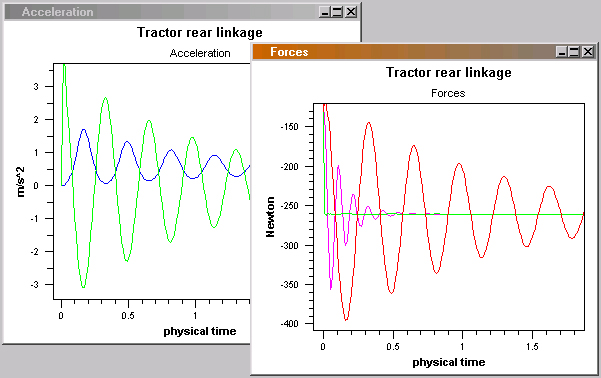
\includegraphics[width=0.86\textwidth]{Figures/graphsCOLOR}
\end{figure}


\def\OutputList{\protect\hyperlink{output-list}{\sl Output List}~}
\SubSection{Output List}{output-list}

The Output List view displays written output from Fedem,
such as a log of commands and solver executions, and error messages.
%This view allows you to observe the commands performed by Fedem.

\vskip\parskip
\IconText{outputList}{To open the Output List view,
  select \textbf{Show Output List} from the \textbf{Windows} menu or tool bar.}

\begin{figure}[H]
  \center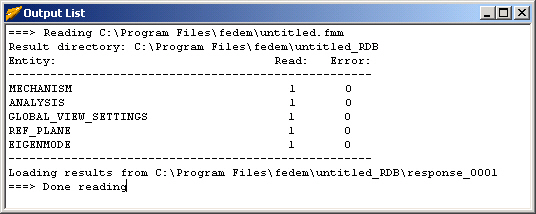
\includegraphics[width=0.8\textwidth]{Figures/Output_List_window_COLOR}
\end{figure}

The text in the Output List view is also written to a log file.
The name of this log file is the same as the current model file name,
but with extension \File {.log} instead of \File{.fmm}.
Therefore, a new log file is opened whenever you \textbf{Open} a
new model, or perform a \textbf{Save As...} command.

\Note{If a log file already exists for the model you open from an earlier
  Fedem session, the output from the current session is appended to that file.
  That means that the entire history of the Output List content for the model
  is recorded. In addition, the date and time of the model open and close
  operations, as well as the Fedem version used, are recorded to the log-file.}


%%%%%%%%%%%%%%%%%%%%%%%%%%%%%%%%%%%%%%%%%%%%%%%%%%%%%%%%%%%%%%%%%%%%%%%%%%%%%%%%
\Section{Executing commands}{executing-commands}

\hskip-33mm
\begin{minipage}{1.4\textwidth}
  \begin{tabular}{p{0.16\textwidth} p{0.49\textwidth} p{0.35\textwidth}}
    \vspace{0pt} 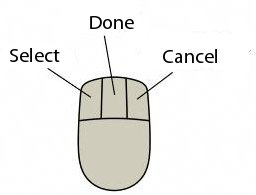
\includegraphics[width=25mm]{Figures/2-mousebuttons} &
    \vspace{0pt} \raggedright
    When performing commands in Fedem, the Guide panel prompts you
    with instructions for completing each command. You may be asked to select
    mechanism objects or locate points to place or move objects.
    Performing commands makes use of three actions:
    \textbf{Select}, \textbf{Done} and \textbf{Cancel}. &
    \vspace{0pt} 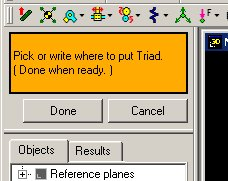
\includegraphics[width=32mm]{Figures/2-Guide}
  \end{tabular}
\end{minipage}

\SubSection{Select}{select}

To select items in your model, or points on objects as references for
moving or creating items, place the cursor over the object or position
and press the left mouse button (left-click). The item is highlighted
and its properties can then be edited in the Property Editor panel.

\Note{Some commands require that an object is selected from views in the
  Workspace area only, such as the Modeler or Control Editor views.
  Instructions regarding these commands are provided in the Guide panel.}

\Tip{To deselect an item, simply click an empty space within the Modeler view.}

\subsubsection{Snapping}

When selecting objects in your model, the selection automatically snaps to
a point on the object such as the nearest node on an FE part, the center point
of a joint, and so on. This makes your selection quick and accurate.

Snapping behaves differently on different types of objects. FE parts, VRML
models, CAD parts and mechanism symbols all have different snapping policies.
Selection snaps to FE nodes on FE parts, to vertices on a VRML part,
to geometry features such as center points and edges on CAD parts,
and to important points on other mechanism symbols.

\subsubsection{Multiple selection}

Some Fedem commands, such as \textbf{Smart Move} and \textbf{Delete},
allow you to select several items at once. To select more than one item,
press and hold down the \textbf{Ctrl} key and then click the items you want
to add to your selection.

If you accidentally add the wrong object to the selection, simply
release the Ctrl key and click an empty space within the Modeler view.
The last selected item is deselected.

\subsubsection{Selection history}

Fedem maintains a history of the items you have selected suring the current
session, which can be accessed using the \textbf{Select Backward} and
\textbf{Select Forward} commands:

\vskip\parskip
\IconText{selectbackward}{To choose a previous selection,
  press the \textbf{Select Backward} button.
  You may need to press it several times to cycle back through the selections
  until the desired object or selection is reached.}

\IconText{selectforward}{To select a recent selection,
  press the \textbf{Select Forward} button once or as many times as necessary
  until the desired selection is reached.}

\subsubsection{Co-located items}

Sometimes several items in a model are located very close together or
on top of each other; in Fedem, these are called co located items.
To select a co located item, click the same spot several times to
cycle through the items. Fedem cycles from the item closest to the viewer to
the one furthest from the viewer.

\subsubsection{Selection Filter}

Some Fedem commands allow you to select only certain types of items.
These restrictions are automatically imposed and based on the type
of command in use. For example, sensors cannot be applied directly to
parts, and Fedem will therefore limit your selection to other types
of mechanism items. To make the selection even easier, you can also
filter the selectable items by limiting the types of items displayed
in the {\sl Modeler view}.

\Tip{To limit the display of mechanism objects, click the
  \textbf{General Appearance} button on the \textbf{Standard} tool bar,
  then disable Mechanism symbols as necessary.
  (See also \refSection{general-appearance}{General Appearance}.)}

\subsubsection{Selecting ground}

To select the ground during modeling,
simply click anywhere on the Reference Plane.

\SubSection{Done}{done}

When executing a command in Fedem, the Guide panel prompts you to select
items or locate points. When you have achieved the desired selection, press
the \textbf{Done} button in the Guide panel to accept it.

\Tip{You can also press the center mouse button within one of the Workspace
  views or the \textbf{Enter} key on the keyboard to accept the selection.}

\SubSection{Cancel}{cancel}

To abort or escape a command procedure,
press the \textbf{Cancel} button on the Guide panel.

\Tip{You can also press the right mouse button within one of the Workspace views
  or the \textbf{Esc} key on the keyboard to cancel a command.}


%%%%%%%%%%%%%%%%%%%%%%%%%%%%%%%%%%%%%%%%%%%%%%%%%%%%%%%%%%%%%%%%%%%%%%%%%%%%%%%%
\Section{Visualizing the model}{visualizing-the-model}

\SubSection{3D Navigation}{navigation}

The 3D navigation commands enables you to change the view without interrupting
the current command or procedure.
There are several different sets of viewpoint control commands:

\begin{itemize}
\item Middle mouse button/wheel + mouse motion
\item Function keys (\textbf{F1}, \textbf{F2}, \textbf{F3}
  and \textbf{F4} + mouse motion)
\item Keyboard keys
\item Predefined view tool buttons
\end{itemize}

\subsubsection{Middle mouse button/wheel}

Pressing and holding the middle mouse button (or wheel if your mouse have that)
while moving the mouse will rotate the view around the rotation center.
If the button/wheel was pressed near the edge of the 3D view, the rotation will
be restricted to the viewport’s normal axis.
Rolling the mouse wheel will zoom in and out. When the mouse wheel is used to
zoom in, the view will be zoomed towards the position of the mouse pointer
giving a combined zoom and pan behavior.
Using the middle mouse button commands is the mostly used 3D navigation method.

\subsubsection{Function keys}

The function key based navigation can be used when you need added control
over the navigation. The commands include:

\begin{itemize}
\item Pan 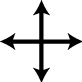
\includegraphics[scale=0.7]{Figures/pan} (\textbf{F1})
\item Zoom 
\includegraphics[scale=0.7]{Figures/zoom} (\textbf{F2})
\item Rotate 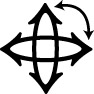
\includegraphics[scale=0.7]{Figures/rotate} (\textbf{F3})
\item Select rotation center
  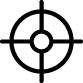
\includegraphics[scale=0.7]{Figures/rotate_center} (\textbf{F4})
\end{itemize}

%These functions are often useful while working in the Modeler view.
%We recommend that you keep your left hand near these function keys while you work.

To use the function key commands, press and hold the function key,
and move the mouse to manipulate the view. The manipulation will only occur
as long as the mouse is inside the Modeler view.
By pressing the left mouse button, you may avoid this restriction.
When the function key is released, the manipulation stops.

\Caution{When pressing the left mouse button while using the function keys,
  Fedem grabs the mouse and keyboard control.}

\subsubsection{Pan - (F1)}

The Pan 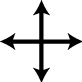
\includegraphics[scale=0.7]{Figures/pan} command shifts the view left,
right, up or down.

\subsubsection{Zoom - (F2)}

The Zoom 
\includegraphics[scale=0.7]{Figures/zoom} command moves the scene
closer or further away from the camera.
It pays attention to the rotation center, and will zoom towards it
(see \protect\hyperlink{select-rotation-center}{\sl"Select rotation center (F4+Select)"} below).
This is useful when you need to examine an object or its components closely.

\Tip{To achieve maximum zoom at a specific point, select the point using
  Select rotation center (\textbf{F4}) and then zoom in on the point using
  Zoom (\textbf{F2}).}

\subsubsection{Rotate - (F3)}

The Rotate 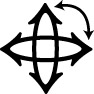
\includegraphics[scale=0.7]{Figures/rotate} command enables you to
dynamically rotate your model around a point or an axis at the rotation center
(see \protect\hyperlink{select-rotation-center}{\sl"Select rotation center (F4+Select)"} below).
The rotation can be performed in two different ways, depending on the position
of the cursor when you press \textbf{F3}.

\begin{itemize}
\item Axis rotation: With the cursor near the edge of the {\sl Modeler view},
  the model rotates around an axis that is perpendicular to the screen.
\item Point Rotation: With the cursor near the center of the view,
  the model rotates around a point located at the rotation center
  some distance into the model. This allows rotation of the model
  in any direction around the point.
\end{itemize}

\Tip{The rotation motion is sensitive to the speed of the mouse.
  If the mouse is moved slowly the control of the rotation becomes finer, and
  makes it possible to accurately control the view along long constructions.}

\SubSubSection{Select rotation center (F4+Select)}{select-rotation-center}

The Select rotation center 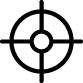
\includegraphics[scale=0.7]{Figures/rotate_center}
command enables you to select a new center for zooming and rotation.
When you use \textbf{F4} to select a point, the selected target point shifts to
the center of the view and becomes the new dynamic center used by the Zoom
(\textbf{F2}) and Rotate (\textbf{F3}) commands.
This target point remains the dynamic center until the model is moved
by some other viewing command.

To select a new rotation point, press and hold down the \textbf{F4} key,
move the cursor to the target point, and click the left mouse button.

\Tip{To closely examine a part of your model, set the dynamic center
  (\textbf{F4}) at the point of interest, and use Zoom (\textbf{F2})
  to magnify the view.
  You can then easily examine the point from many directions using Rotate
  (\textbf{F3}).}

\subsubsection {Keyboard keys}

To rotate the model by increments of 15 degrees, use the arrow keys.
Rotation and panning may also be done by pressing \textbf{Shift}
(rotate 90 degrees), \textbf{Alt} (rotate around screen normal) or
\textbf{Ctrl} (panning) in combination with arrow keys.
To zoom in and out, press \textbf{z} or \textbf{Shift + z}.


\SubSection{Predefined view tool buttons}{predefined-view-tool-buttons}

Fedem provides the following commands for some predefined view settings:

\vskip\parskip
\IconText{isometricView}{\textbf{Isometric}\newline
  To display an isometric view of your mechanism, click the \textbf{Isometric} button.}

\vskip\parskip\IconText{viewTop}{\textbf{Top}\newline
  To display the top view of your mechanism, click the \textbf{Top} button.}

\vskip\parskip\IconText{viewRight}{\textbf{Right}\newline
  To display the side view of your mechanism, click the \textbf{Right} button.}

\vskip\parskip\IconText{viewFront}{\textbf{Front}\newline
  To display the front view of your mechanism, click the \textbf{Front} button.}

\vskip\parskip\IconText{viewBottom}{\textbf{Bottom}\newline
  To display the bottom view of your mechanism, click the \textbf{Bottom} button.}

\vskip\parskip\IconText{viewLeft}{\textbf{Left}\newline
  To display the left side view of your mechanism, click the \textbf{Left} button.}

\vskip\parskip\IconText{viewBack}{\textbf{Back}\newline
  To display the back view of your mechanism, click the \textbf{Back} view button.}


\SubSection{3D View Controls}{view-controls}

Fedem provides several 3D viewing commands for use in the {\sl Modeler} view.
The following commands can be accessed on the {\textbf 3D View Control} tool bar
(or from the \textbf{View} menu):

\vskip\parskip\IconText{solidView}{\textbf{Solid View}\newline
  To display all mechanism items as solid/shaded objects,
  click the \textbf{Solid View} button. This is on by default.}

\vskip\parskip\IconText{lineView}{\textbf{Line View}\newline
  To speed up graphic performance and display all mechanism items as outlines,
  click the \textbf{Line View} button.}

\vskip\parskip\IconText{flatShading}{\textbf{Flat Colors}\newline
  To render the model without shading, click the \textbf{Flat Colors} button.
  This is especially useful when viewing color plots.
  This option is off by default.}

\vskip\parskip\IconText{showTopFaces}{\textbf{Show Top Faces}\newline
  To distinguish the top and bottom faces of shell elements,
  click the \textbf{Show Top Faces} button. The top faces will then be rendered
  normally while the bottom faces will be rendered dark/black. If some of the
  parts have the detail level set to Reduced Surface or Reduced Surface and
  Internals, only a rough indication on the states of the faces is given.
  To see the exact top and bottom of every face on a part, set the detail level
  to Surface or Surface and Internals. This is off by default.}

\vskip\parskip\IconText{perspectiveView}{\textbf{Perspective}\newline
  To display a perspective view of your mechanism,
  click the \textbf{Perspective} button. This command controls the appearance
  of mechanisms in depth as perceived by normal binocular vision.}

\vskip\parskip\IconText{parallelView}{\textbf{Parallel Projection}\newline
  To display a parallel view of your mechanism,
  click the \textbf{Parallel Projection} button.}


\SubSection{Zoom and Pan}{zoom-and-pan}

Fedem provides zooming and panning controls for use in the active view.
The following commands can be accessed on the \textbf{Zoom and Pan} tool bar
(or from the \textbf{View} menu):

\Note{Some of these commands cannot be used in all views.
  When commands cannot be used in the current view, their buttons become
  unavailable (grayed out) on the menus and tool bars.}

\vskip\parskip\IconText{zoomAll}{\textbf{Zoom All}\newline
  To scale the active view so that all objects (for {\sl Graph} views,
  every Curve on the Graph) fit within the view, press the \textbf{Zoom All}
  button. When working in {\sl Graph} views, this can also be achieved by
  pressing the \textbf{F5} key.}

\vskip\parskip\IconText{zoomWindow}{\textbf{Zoom Window}\newline
  To enlarge a rectangular area, press the \textbf{Zoom Window} button.
  The command can also be activated by pressing the \textbf{Z} key.}

\vskip\parskip\IconText{zoomTo}{\textbf{Zoom To}\newline
  This command pops up the correct view, zooms to the selected object,
  and places the Dynamic Center of rotation at the center of the object.
  This is useful when trying to locate a certain Triad or Joint in large models.
  This command is also available from the {\sl Topology} view and the
  Model Manager panel (see \refSection{model-manager}{Model Manager}
  and \refSection{id-and-topology-panel}{ID and Topology panel}).
  It is also applicable on Control Elements and Control Lines in the
  {\sl Control Editor} view (see \refSection{control-editor}{Control Editor}).}

% This feature vanished with the Qwt-porting years ago
%\vskip\parskip\IconText{zoomWindowAutoscale}{
%  \textbf{Zoom Window with Autoscale}\newline
%  To enlarge a rectangular area, press the \textbf{Zoom Window With Autoscale}
%  button. The contents will be auto scaled to fit the entire plotting area.
%  This command can also be activated by pressing the \textbf{X} key.}

\vskip\parskip\IconText{zoomIn}{\textbf{Zoom In}\newline
  To enlarge the active view by a predefined scale factor,
  press the \textbf{Zoom In} button.}

\vskip\parskip\IconText{zoomOut}{\textbf{Zoom Out}\newline
  To reduce the active view by a predefined scale factor,
  press the \textbf{Zoom Out} button.}

\vskip\parskip\IconText{panLeft}{\textbf{Pan Left}\newline
  To move the active view to the left, press the \textbf{Pan Left} button.}

\vskip\parskip\IconText{panRight}{\textbf{Pan Right}\newline
  To move the active view to the right, press the \textbf{Pan Right} button.}

\vskip\parskip\IconText{panUp}{\textbf{Pan Up}\newline
  To move the active view up, press the \textbf{Pan Up} button.}

\vskip\parskip\IconText{panDown} {\textbf{Pan Down}\newline
  To move the active view down, press the \textbf{Pan Down} button.}


\SubSection{General Appearance}{general-appearance}

The \textbf{General Appearance} command can be used to control which entities
are displayed in the {\sl Modeler} view. This command also provides control of
the size and appearance of mechanism symbols.

\vskip\parskip
\IconText{generalAppearance}{Click the \textbf{General Appearance} button
  to open the associated dialog box (shown below).}

\clearpage
\noindent
\begin{minipage}{0.6\textwidth}
  \raggedright
  \begin{bulletlist}
  \item{\sl Mechanism symbols} --
    allows you to toggle on/off the display of mechanism items
    of different type, to edit the color used to specify each item type,
    and to change the size of symbols and line width
    (see \protect\hyperlink{mechanism-symbols}{\sl"Mechanism symbols"} below).
  \item{\sl Default colors} --
    controls the colors used for Grounded Triads,
    unattached mechanism items and the Modeler background
    (see \protect\hyperlink{default-colors}{\sl"Default colors"} below).
  \item{\sl Viewer options} --
    controls 3D rendering options such as visibility, transparency type,
    and line-smoothing
    (see \protect\hyperlink{viewer-options}{\sl"Viewer options"} below).
  \end{bulletlist}
\end{minipage}% <--- the % is needed here to kill off  spurious spacing
\begin{minipage}{0.4\textwidth}
  \raggedleft
  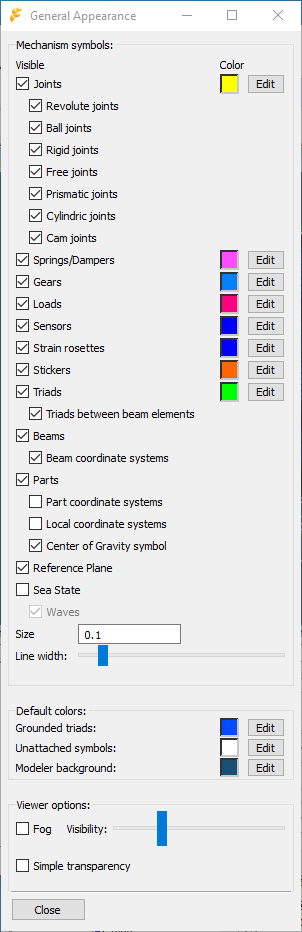
\includegraphics[trim=0 400 0 0,clip,scale=0.55]{Figures/Dialogs/2-GeneralAppearance}
\end{minipage}

\SubSubSection{Mechanism symbols}{mechanism-symbols}

This area provides the following controls:

\noindent
\begin{minipage}{0.6\textwidth}
  \raggedright
  \begin{itemize}
  \item{\sl Visible} --
    enables/disables the display of each item type.
    Click the box next to an item type to change the setting. The toggles that
    are indented slightly to the right are considered as sub-types of the item
    toggle just above them. They are active only if that toggle is enabled.
    \vskip1mm
    \MiniGenericNote{tip}{TIP}{-30mm}{1.83}{0.173}{0.48}{
      Turning off visualization of items speeds up and simplifies the display
      of complex mechanisms, and provides a useful way to limit the selection
      to specific item types.}
  \end{itemize}
\end{minipage}% <--- the % is needed here to kill off spurious spacing
\begin{minipage}{0.4\textwidth}
  \raggedleft
  \begin{picture}(125,173)
    \put(0,0){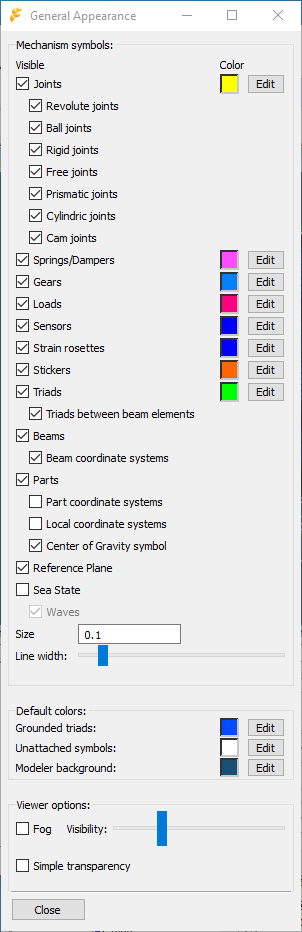
\includegraphics[trim=0 0 0 300,clip,scale=0.55]{Figures/Dialogs/2-GeneralAppearance}}
    \put(-10,362){\Bullet{1}}
    \put(-10,87){\Bullet{2}}
    \put(-10,47){\Bullet{3}}
  \end{picture}
\end{minipage}

\noindent
\begin{minipage}{0.6\textwidth}
  \raggedright
  \begin{itemize}
  \item{\sl Color} --
    allows editing of the RGB settings for each item type.
    Press the \textbf{Edit} button next to an item type to edit the default
    display color for that item type. In the appearing dialog box
    (shown at right), move the sliders to change the settings or enter
    the desired values directly in the number fields.
  \end{itemize}
\end{minipage}% <--- the % is needed here to kill off spurious spacing
\begin{minipage}{0.4\textwidth}
  \raggedleft
  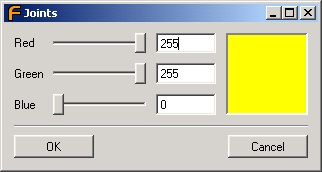
\includegraphics[scale=0.52]{Figures/Dialogs/2-Color}
\end{minipage}

\clearpage
\begin{itemize}
\item{\sl Size} --
  a scale factor for sizing the display of mechanism entities.
  To change the size of items, enter a new number in the size field.
\item{\sl Line Width} --
  this is a scale factor for the line width of all mechanism symbol lines,
  together with all 1D elements and Surface Connectors in the FE parts
  (see \refSection{surface-connectors}{Surface Connectors}).
  To change the line-width, move the slider right or left.
\end{itemize}

\SubSubSection{Default colors}{default-colors}

This area enables the user to edit the colors used on the modeling background
and unattached mechanism items. It also allows you to set the colors on Triads
that are attached to the Ground, to distinguish them from Triads that are free
to move. The default colors may be changed in a similar ways as changing the
colors for \protect\hyperlink{mechanism-symbols}{\sl Mechanism symbols}.

\SubSubSection{Viewer Options}{viewer-options}

This area enables the user to modify the way that models are rendered.

\begin{itemize}
\item{\sl Fog} is an option that enables you to create a fog-like effect around
  your model that appears as fog or darkness (or even an underwater scene).
  The distant parts of the model appear to fade into the background.
  The Visibility slider controls the distance at which the model is completely
  hidden in the fog.
 \item{\sl Simple Transparency} is a dithering algorithm used to speed graphic
   performance when displaying transparent objects in your model.
   The effects of this option depend on the type of graphics card you have.
 \item{\sl Anti-Aliasing} enables/disables line-smoothing for symbols.
\end{itemize}

\Tip{You can create the following effects with the Fog option:
  \begin{itemize}
  \item To create the effect of a foggy day, set the Modeler background color to
    light gray (Red 180, Green 180, Blue 180), enable the Fog option, and adjust
    the Visibility slider until the model almost fades into the background.
  \item To create the effect of an underwater scene, set the Modeler background
    color to sea green (Red 20, Green 125, Blue 130), enable the Fog option,
    and adjust the Visibility slider until the model nearly
    fades into the background.
  \end{itemize}}

\Tip{If Anti-Aliasing does not function properly,
  try enabling the Simple Transparency option.}

\Note{Graphics cards do not all have the same optimal settings.
  In general, disabling the Fog and Anti-Aliasing options and turning on
  Simple Transparency gives the best performance, but with some systems the
  performance gain is insignificant.}


\SubSection{Item Appearance}{item-appearance}

The \textbf{Item Appearance} command can be used to change the level of detail
and the appearance of individual Parts and the Reference Plane.

\IconText{itemAppearance}{To open the Item Appearance dialog box (shown below),
  click the \textbf{Item Appearance} button on the \textbf{Standard} tool bar,
  and select a Part or the Reference Plane for which you want to change the
  appearance of.}

\Tip{To change the appearance of a hidden Part, select the Part in the
  {\sl Objects} list of the Model Manager panel, after clicking the
  \textbf{Item Appearance} button.}

\noindent
\begin{minipage}{0.55\textwidth}
  \raggedright
  \begin{bulletlist}
  \item{\sl Level of Detail} --
    controls the level of complexity displayed in the model.
    The {\sl Polygons} and {\sl Lines} settings allow you to change
    the complexity of models displayed in the {\sl Modeler} view,
    (see \protect\hyperlink{level-of-detail}{\sl"Level of Detail"} below).
    Changing these settings can improve the graphic performance of 3D rendering.
  \item{\sl Color} --
    controls the RGB settings of the selected Part or Reference Plane.
  \item{\sl Material} --
    controls the shininess and transparency of the selected Part
    or Reference Plane.
  \end{bulletlist}
\end{minipage}% <--- the % is needed here to kill off spurious spacing
\begin{minipage}{0.45\textwidth}
  \raggedleft
  \begin{picture}(136,180)
    \put(0,0){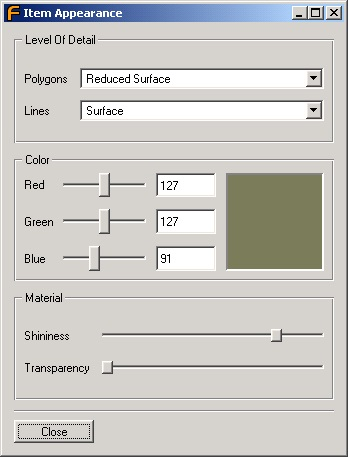
\includegraphics[scale=0.52]{Figures/Dialogs/2-ItemAppearance}}
    \put(-5,158){\Bullet{1}}
    \put(-5,112){\Bullet{2}}
    \put(-5,56){\Bullet{3}}
  \end{picture}
\end{minipage}

\SubSubSection{Level of Detail}{level-of-detail}

Polygons can be displayed at five levels of detail:
Surface and Internals, Reduced Surface and Internals,
Surface, Reduced Surface, and Off. The default level is Surface.

\begin{enumerate}
\item{\sl Surface and Internals} --
  With polygon detail set to Surface and Internals,
  element faces from solid elements inside the parts are shown
  together with the surface faces of the elements.
  All element faces are shown as single polygons.
\item{\sl Reduced Surface and Internals} --
  Setting the detail level to Reduced Surface and Internals displays
  a simplified polygon representation of the surface and internals of a part.
  This is faster than using Surface and Internals,
  but shows a less accurate representation of the parts.
\item{\sl Surface} --
  This option turns off the internal faces in a part,
  and will only show the surface element faces of a part.
  All the surface faces are shown as separate polygons.
\item{\sl Reduced Surface} --
  Setting the polygon detail to Reduced Surface provides the most efficient way
  to visualize the shaded view of a mechanism part.
  The surface is displayed using a simplified polygon model
  and the internal faces are turned off.
\item{\sl Off} --
  Setting the polygon detail to Off turns all polygons off.
\end{enumerate}

Lines can be displayed at six levels of detail: Full, Surface, Outline, Outline
No 1D-elements, Simplified, and Off. The default level is Outline.

\begin{enumerate}
\item{\sl Full} --
  With line detail set to Full, mesh lines from solid elements inside the parts
  are shown together with the surface mesh of the elements.
\item{\sl Surface} --
  Setting the line detail level to Surface displays only the mesh lines
  on the surface of the FE model.
\item{\sl Outline} --
  This option leaves only the mesh lines on the surface of the part with
  neighboring element faces with a relative face-angle above a given threshold.
  The default threshold is $\pi/4$. (It is possible to edit this
  value for each part by editing the model file.)
\item{\sl Outline No 1D-elements} --
  Same as {\sl Outline} except that all Surface Connectors and 1-D elements,
  such as RGD, WAVGM, BEAM2, are also removed from the display.
\item{\sl Simplified} --
  This option generates a simple line visualization of the part
  based on the Triads attached to it.
  One line is drawn from each Triad to their geometrical center.
  This option makes most sense if the polygons are turned off.
  This visualization is the same that is used if the part is not loaded,
  see \refSection{fe-data-settings}{FE-Data Settings}.
\item{\sl Off} --
  Setting the line detail to Off turns all mesh lines off.
\end{enumerate}

\Tip{To edit the appearance or level of detail on several parts
  at the same time, select multiple parts in the Objects list in the
  Model Manager panel, after clicking on the Item Appearance icon.}


\SubSection{Element face visibility}{element-face-visibility}

The visibility of elements can be controlled using the commands
\textbf{Hide Element Faces} and \textbf{Show Element Faces} in the right-click
menu in the {\sl Objects} list of the Model Manager panel.
These commands can be applied to the entire part, or to a selection of the
element groups listed in the {\sl Objects} list.
The icon in front of each group entry in the list indicates the current visual
state of the elements in that group:
Either all visible 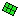
\includegraphics[scale=0.8]{Figures/AllElementsVisible},
some visible 
\includegraphics[scale=0.8]{Figures/SomeElementsVisible}
or all hidden 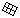
\includegraphics[scale=0.8]{Figures/AllElementsHidden}.

These commands will only be active when the polygon detail level is set to
Surface or Surface and Internals, or when color contour results are loaded for
the Part. This feature can also be utilized to load color contour results only
for small parts of a big Part because the color values will not be loaded on
hidden elements. See also
\refSection{performance-of-animation-loading}{Performance of animation loading}.

\Note{The visibility of the mesh is not affected by the
  \textbf{Show}/\textbf{Hide} commands.}


\SubSection{Visualization of special elements}{visualization-of-special-elements}

There are several element types that are treated differently from normal elements
like shells and solids, when it comes to visualization. Those elements are
listed in the table below.

\begin{table}[h!]
\begin{tabular}{ | m{33mm} | m{25mm}| m{45mm} | }
 \hline
 Element type & Visualization & Comments \\
 \hline\hline
 Beams & Dash dot lines & Any eccentricity is shown as dotted lines from the nodal point to the beam end \\
 \hline
 Rigid bars & Dashed lines & \\
 \hline\raggedright
 Constraint elements (RBE3, WAVGM, Distributed coupling) & Dotted lines &  \\
 \hline
 Concentrated mass & No visualization & \\
 \hline
 Springs & No visualization &  \\
 \hline
 Bush elements & No visualization & \\
 \hline
\end{tabular}
\end{table}

\subsubsection{Color}

The color of those elements are set automatically to black, white or a
grayish color to achieve a good contrast to both the color of the part,
and the viewer background. If the FE part is displayed using lines only,
the color of those elements is set to the color of all the other lines.

\subsubsection{Line width}

The line width is adjusted according to the Line Width parameter set
for the Mechanism symbols.
See \refSection{general-appearance}{General Appearance}.


\SubSection{Measuring distance and angles in a model}{measuring-distance-and-angles}

Sometimes during the modeling of complex mechanisms, it is necessary or
convenient to quickly assess the distance between two arbitrary points
in the model or to measure the angle between two lines. For this purpose,
two command are available from the \textbf{Tools} menu.

\vskip\parskip
\IconText{distance}{Select \textbf{Measure distance...} to check the
  distance between two points. Then click on two points in the {\sl Modeler}
  view to output their global positions and the relative distance between them
  in the \OutputList view.
  You can repeat to click on two new points to check their relative
  distance as many times you like. Press \textbf{Cancel} to quit the command.}

\begin{figure}[H]
  \center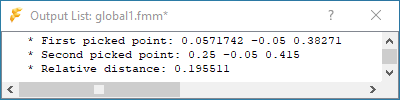
\includegraphics[scale=0.8]{Figures/2-OutputListDistance}
\end{figure}

\IconText{angle}{Select \textbf{Measure angle...} to check the
  angle between two lines defined through three selected points.
  The end points of the two lines are selected first by clicking on two
  arbitrary locations in the {\sl Modeler} view, followed by the common start
  point of the two lines.
  The global positions of the three selected points, as well as the angle
  (in radians) rotating the line though the third and first point into the line
  through the third and second are then shown in the \OutputList view.
  You can repeat to click on three  new points to measure more angles as many
  times you like. Press \textbf{Cancel} to quit the command.}

\begin{figure}[H]
  \center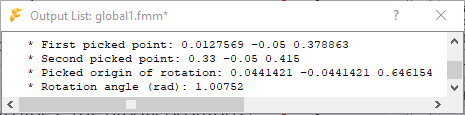
\includegraphics[scale=0.7]{Figures/2-OutputListAngle}
\end{figure}


%%%%%%%%%%%%%%%%%%%%%%%%%%%%%%%%%%%%%%%%%%%%%%%%%%%%%%%%%%%%%%%%%%%%%%%%%%%%%%%%
\Section{Opening and saving model files}{opening-and-saving-model-files}

\SubSection{Opening a file}{opening-a-file}

You can open a Fedem model file created in this version
(or any of the previous versions) of Fedem through the following steps:

\vskip\parskip
\IconText{open}{\vskip-5mm
  \begin{enumerate}
  \item Chose \textbf{Open...} in the File menu,
    or use the \textbf{Open} icon in the tool bar,
    to make the Open model file dialog box appear (shown below).
  \item Locate the wanted Fedem model in the dialog box and click \text{Open}.
\end{enumerate}}
\vskip-5mm

\begin{figure}[H]
  \center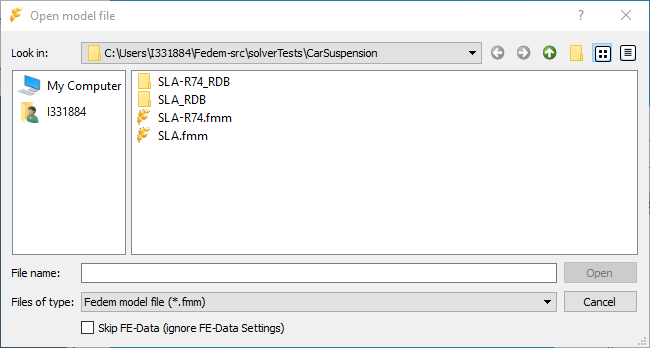
\includegraphics[scale=0.62]{Figures/Dialogs/2-Open}
\end{figure}

The Open model file dialog box normally displays all files with the Fedem model
file extension (\File{.fmm}). However, you may open a file with any extension by
selecting the All files filter in the File of type pull-down menu.

\Caution{If you choose to open a file without the \File{.fmm} extension,
  you should make sure it is a proper Fedem model file.
  Attempting to open a non-model file will usually result in an empty model,
  but unpredictable behavior may also occur, depending on the actual contents
  of the file.}

You can skip the loading of FE data for the parts if the model contains
large parts that take a long time to load. See also
\refSection{skipping-fe-data-when}{Skipping FE-Data when opening a model file}.

If the opened model file contains results, information about the
result files in the model (.frs files) is reported in the \OutputList view.
However, results files belonging to unloaded parts
(see \refSection{loading-and-unloading-fe-data}{Loading and unloading FE-Data})
and disabled result files
(see \refSection{result-manipulation}{Result manipulation})
are not included in this report.

If any problems are encountered during model loading, Fedem displays
a message box and provides additional information in the \OutputList view.

\Note{There might be minor changes in the model file format from one
  Fedem version to subsequent versions of Fedem.
  The newer versions are always backward compatible such that you may
  safely open a model that was created in one particular version in any
  of the subsequent versions, without loosing model consistency.
  The model is automatically converted to the new format while reading it.}

\Caution{The Fedem model files are not necessarily forward compatible.
  If you open a model in an older version of Fedem than it was created in,
  there might be changes in the model file format that makes the imported model
  incorrect or inconsistent.
  In some cases it may also make the Open operation fail or hang.
  Refer to the Fedem R5.0 Release Notes, Chapter 3, "Notes",
  for a summary of the forward compatibility issues that might need to
  be manually resolved in such cases.}

\subsubsection{Loading parts}

When Fedem opens a model file and the loading of FE data is enabled,
the part information (\File{.ftl} files, reduced matrix files, etc.)
is read from the FE model repository,
see \refSection{using-fe-model-repositories}{Using FE model repositories}.

If the FE model repository is missing, for example when a model
file is moved, Fedem uses the following search path to locate the parts:

\begin{enumerate}
\item The name and location of the originally imported FE part.
\item The name of the original FE part, located in a sub-directory
  of the current model file directory, with the same name as in the
  original FE file path (only if the original path was an absolute path).
\item The name of the original FE part, located in a parallel
  directory of the current model file directory, with the same name as in the
  original FE file path (only if the original path was an absolute path).
\item The name of the original FE part, located in the same
  directory as the model file.
\item The base name of the original FE part with the extension \File{.ftl}
  located in the same directory as the model file.
\end{enumerate}

\clearpage
\SubSection{Saving models}{saving-models}

To save the current model, do one of the following:

\vskip\parskip
\IconText{save}{\vskip0pt
  \begin{itemize}
  \item To replace the current version on disk,
    choose \textbf{Save} in the \textbf{File} menu or
    click on the \textbf{Save} icon in the tool bar.
  \item To save the file in a different location and/or with a different name,
    choose \textbf{Save As...} in the \textbf{File} menu.
  \end{itemize}}

\vskip-5mm
\Note{The previous version of the model file will be renamed to
  \File{\Variable{filename}.bak} before saving the model to the same file,
  such that you can always go back to the previously saved version by renaming
  that file, in case the last save operation failed due to full disk
  or other reasons.}

When saving a copy of the model using the \textbf{Save As...} command,
a dialog box labeled "Save model file as" appears (shown below),
in which you can choose the new file name. Here you can also choose
to \textbf{Discard reduced FE models} by enabling the associated toggle
(this toggle is present only when the model contains FE parts).

\begin{figure}[H]
  \center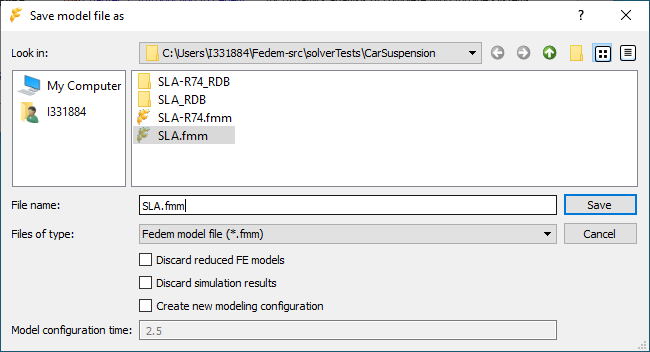
\includegraphics[scale=0.6]{Figures/Dialogs/2-SaveAsUpdated}
\end{figure}

When saving a new model for the first time, you are prompted to give it a name
different from the default name \Untitled, which was assigned when
Fedem was started (see \refSection{starting-fedem}{Starting Fedem}).
If you also have performed some solver tasks before saving the model,
the existing results database will then be moved to the correct location
associated with the new model file name, unless you have toggled on either
Discard simulation results or \textbf{Create new modeling configuration}, see
\protect\hyperlink{saving-a-model-copy-with-results}
                  {\sl"Saving a model copy with results"} below.

\Caution{If you do not save a new model still named \Untitled{}
  before you open another model or Exit Fedem,
  all solver results associated with this model will be deleted, if any.
  This also includes the results of any reductions performed,
  unless FE model repositories were used
  (see \refSection{using-fe-model-repositories}{Using FE model repositories}).}

\SubSubSection{Saving a model copy with results}
              {saving-a-model-copy-with-results}

If the model contains simulation results when you do a \textbf{Save As...},
you will have the options to either \textbf{Discard simulation results} or
\textbf{Create new modeling configuration}, by activating the
associated toggles:

\begin{figure}[H]
  \center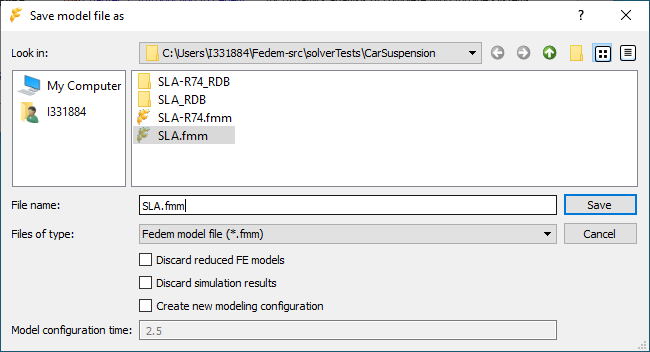
\includegraphics[scale=0.6]{Figures/Dialogs/2-SaveAsUpdated}
\end{figure}

If the latter toggle is activated, you can then specify the simulation
time from which the response state will be used to create a
new modeling configuration, by updating all Triad and Part
positions in the new model.

\subsubsection{Indication on whether a Save is needed}

\begin{wrapfigure}{r}{0.4\textwidth}
  \includegraphics[width=0.4\textwidth]{Figures/2-TitleWithAsterisk}
\end{wrapfigure}

When the current model has been changed compared to the previously saved
version, Fedem will indicate this with an asterisk (*) after
the model file name in the title bar of the main window.
Only if this asterisk is present, you will be asked if you
first want to save the current model when you \textbf{Open} another model,
create a \textbf{New} model, or \textbf{Exit}.


\SubSection{Starting a new model}{starting-a-new-model}

You can at any time during a Fedem session start modeling on a new model.

\IconText{new}{Choose \textbf{New} from the \textbf{File}
  menu, or click the \textbf{New} icon in the tool bar.
  This is equivalent to exiting the current Fedem session and then starting
  a new one (see \refSection{starting-fedem}{Starting Fedem})
  except that the new model now by default will be located in the same directory
  as the current model.}

\Note{If the current model has been modified after the last \textbf{Save},
  you will be asked whether you want to save those changes
  before starting on the new model.}


%%%%%%%%%%%%%%%%%%%%%%%%%%%%%%%%%%%%%%%%%%%%%%%%%%%%%%%%%%%%%%%%%%%%%%%%%%%%%%%%
\Section{Loading and unloading FE-data}{loading-and-unloading-fe-data}

When a model contains several large FE-models, unloading some of the FE-data
from memory can be necessary to in order to reduce the amount of resources used.
This is particularly useful when you want to load contour plots for a
particular part, or to free up resources for the solvers.


\SubSection{FE-data settings}{fe-data-settings}

FE models often tend to be large.
The amount of data needed for visualization and lookup is indeed significant.
In some cases it will be convenient or necessary to unload this data,
to free up RAM.

\IconText{FE-DataSettings}{To control the loading and unloading of FE-data, the
  FE-Data Settings dialog box is used. To open this dialog box (shown below),
  select the \textbf{FE-Data Settings...} command in the \textbf{Tools} menu.}

\begin{wrapfigure}{R}{0.5\textwidth}
  \includegraphics[width=0.5\textwidth]{Figures/Dialogs/2-FE-DataSettings}
\end {wrapfigure}

The status of each FE part is set using the pull-down menu in the {\sl Status}
column. Set the status you want for each part,
and press \textbf{OK} or \textbf{Apply}.
The parts that are not loaded will be shown using the Simplified line shape,
as described in \refSection{item-appearance}{Item Appearance}.

The loading and unloading of FE parts does not affect the simulation.
The solver processes will read the necessary FE-Data from the FE-model files.

\Tip{To change the status of all or several parts quickly, it is convenient to
  use the arrow keys to navigate between the pull-down menus, and the
  \textbf{N} key (Not Loaded) or \textbf{L} key (Loaded) to set the status.}

\Note{Loading unloaded parts can take several minutes if the parts are big.}


\SubSection{Skipping FE-data when opening a model file}{skipping-fe-data-when}

When opening a big model for inspection or simulation, it is sometimes
convenient to override the FE-Data Settings and skip the FE-models
completely. In that way you can open a model containing extremely large
parts in a few seconds, without using any significant amount of memory.

To do this, toggle the {\sl Skip FE-Data} toggle in the Open model file dialog
box when opening a model file, or use the \File{-noFEData} command-line option
together with \File{-f \Variable{modelfilename}} when starting Fedem.

The model will then be loaded with all FE parts unloaded. To load the parts,
open the FE-Data Settings dialog box which now will show the status on the
parts last time you saved your model. If you simply press \textbf{OK} or
\textbf{Apply}, those settings will be applied and the parts that was marked as
{\sl Loaded} will then actually be loaded.


\SubSection{Modeling with unloaded parts}{modeling-with-unloaded-parts}

An unloaded part can generally be used as any other part while modeling,
but there are some restrictions.
When selecting points on the part, the points will not snap to the closest node
because the node information has not been loaded.
The only points on the part that are available for selecting and modeling are
the external nodes represented by the Triads.

Triads can generally not be detached or deleted from unloaded FE parts.
This is done to protect the reduced matrices associated with the part
from being accidentally invalidated.
If you try to to do this, you will instead get an error message instead.
When detaching a Joint from an unloaded FE part,
a Triad will be left on the part where the Joint was attached.


\SubSection{Postprocessing unloaded parts}{postprocessing-unloaded-parts}

Unloaded FE parts will be completely skipped when loading an Animation,
except for the rigid body motion. This makes it possible to focus the
computer resources on the parts of your model that are interesting,
and skip everything else, see also
\refSubSection{disabling-and-enabling}{Disabling and Enabling results}
{result-manipulation}.


%%%%%%%%%%%%%%%%%%%%%%%%%%%%%%%%%%%%%%%%%%%%%%%%%%%%%%%%%%%%%%%%%%%%%%%%%%%%%%%%
\Section{Exporting objects}{exporting-objects}

Fedem can export six types of objects: Parts (FE models), individual
Curves, Graphs, Graph views, the Modeler view and Animations.

\begin{itemize}
\item FE Parts can be exported in Fedem Technology Link (\File{.ftl}) format.
\item Curves and Graphs can be exported in ASCII (\File{.asc}, \File{.txt}),
  nCode DAC (\File{.dac}) or MTS RPC time history (\File{.rsp}, \File{.drv},
  \File{.tim}) format.
\item The Modeler- and Graph views can be exported as binary image files
  in a variety of formats.
\item Animations can be exported as movies
  in \File{.mpeg} and \File{.avi} formats.
\end{itemize}


\SubSection{Exporting a part}{exporting-a-part}

To export an FE Part, complete the following steps:

\noindent
\begin{minipage}{0.65\textwidth}
  \raggedright
  \begin{enumerate}
  \item Right-click the part in the Model Manager {\sl Objects} list to access
    the shortcut menu (partly shown right).
  \item Select \textbf{Export Part...} to open the \newline
    ``Save part as'' dialog box.
  \item Specify a file name and location, \newline
    then click \textbf{Save}.
  \end{enumerate}
\end{minipage}% <--- the % is needed here to kill off spurious spacing
\begin{minipage}{0.35\textwidth}
  \raggedleft
  \includegraphics[trim=0 35 0 20,clip,width=\textwidth]{Figures/2-ExportPart}
\end{minipage}


\SubSection{Exporting curves and graphs}{exporting-curves-and-graphs-2}

To export curves, complete the following steps:

\noindent
\begin{minipage}{0.5\textwidth}
  \raggedright
  \begin{enumerate}
  \item Select one or more Curves in the Model Manager {\sl Results} list,
    and right-click your mouse to access the shortcut menu (shown right).
  \item Select \textbf{Export Curves...} to open the dialog box labeled either
    ``Save curve as'' or ``Save curves to directory''.
  \item Depending on your selection, you will be prompted for either a
    file name or a directory.
    If you select multiple curves, the curve files will be named automatically,
    \newline but you have to select what file format you want to export to.
  \end{enumerate}
\end{minipage}% <--- the % is needed here to kill off spurious spacing
\begin{minipage}{0.5\textwidth}
  \raggedleft
  \includegraphics[width=0.95\textwidth]{Figures/2-ExportCurves}
\end{minipage}

To export one or more graphs, complete the following steps:

\begin{enumerate}
\item Select one or more graphs or curves in the Model Manager {\sl Results}
  list and right-click your mouse to access the shortcut menu.
\item Select \textbf{Export} and then \textbf{Export Graphs...} to open the
  dialog box labeled either ``Save graph as'' or ``Save graph to directory''.
\item As when exporting curves, you will be prompted for either a file name
  or a directory depending on your selection. The graph files will be given
  names automatically if you have selected multiple graphs.
\end{enumerate}

For more detailed information on how to export and import curves and
graphs, see \refSection{export-of-curve-data}{Export of Curve Data}
and \refSection{importing-curves-and-graphs}{Importing Curves and Graphs},
respectively.


\SubSection{Exporting the 3D modeler view}{exporting-the-3d-modeler-view}

\noindent
\begin{minipage}{0.41\textwidth}
  \setlength{\parskip}{1mm}
  \raggedright
  To export this view, make it active, then select \textbf{Export} and then
  \textbf{Export View...} from the \textbf{File} menu.

  When exporting the {\sl Modeler} view, you may choose between the following
  image formats:

  \begin{itemize}
  \item\File{.bmp}
  \item\File{.jpeg}
  \item\File{.png}
  \item\File{.rgb}
  \item\File{.iv} \small(3D inventor snapshot)
  \end{itemize}
\end{minipage}% <--- the % is needed here to kill off spurious spacing
\begin{minipage}{0.59\textwidth}
  \raggedleft
  \includegraphics[width=0.95\textwidth]{Figures/2-ExportView}
\end{minipage}

\vskip5mm
The different file formats have different quality.
The format \File{.jpeg} is widely recognized.
The compression reduces the quality somewhat, but the files are small.
The formats \File{.png} and \File{.bmp} have better quality.
We recommend using the \File{.png} format for high quality images.

The \File{.iv} format enables dynamic 3D-viewing of your models using
an external viewer. Viewers are available for several platforms.

Stills of animations, e.g., contour plots, can also be exported.
Simply pause your animation where you want the picture or 3D-snapshot taken,
then export the {\sl Modeler} view.


\SubSection{Exporting graph views}{exporting-graph-views}

To export a {\sl Graph} view, follow the steps described in the section above.
Here you may choose between these image formats:

\begin{itemize}
\item\File{.bmp}
\item\File{.jpeg}
\item\File{.png}
\end{itemize}


\SubSection{Exporting animations}{exporting-animations-intro}

\begin{wrapfigure}{R}{0.5\textwidth}
  \includegraphics[width=0.5\textwidth]{Figures/2-ExportAnim-sec-2-8-2}
\end {wrapfigure}

Animations can be exported using the \File{.mpeg} (mpeg-1 or mpeg-2) and
\File{.avi} (Windows only) formats. The exported animation may be viewed
in any standard video player, e.g., Windows Media Player or Elecard MPEG
Player (www.elecard.com).

After loading the animation, select \textbf{Export} and then
\textbf{Export Animation...} from the \textbf{File} menu to open a dialog box
where you can select location, file name and format of your exported animation.
See \refSection{exporting-animations}{Exporting animations} for details.

\clearpage


%%%%%%%%%%%%%%%%%%%%%%%%%%%%%%%%%%%%%%%%%%%%%%%%%%%%%%%%%%%%%%%%%%%%%%%%%%%%%%%%
\Section{Customizing Fedem using Plug-Ins}{customizing-fedem-using-plug-ins}

On Windows, plug-ins are provided as DLL-files in the \File{plugins} subfolder
of the installation folder of the Fedem software. Once a plug-in DLL has been
placed in the \File{plugins} folder, it will show up in the Plug-Ins dialog box
in Fedem (see below), which is available from \textbf{Tools} menu.
Here you can tick which plug-ins to use.

\begin{figure}[!h]
  \center\includegraphics[width=0.6\textwidth]{Figures/Dialogs/2-Plugins}
\end{figure}

Fedem currently provides plug-in interfaces of two kinds; user-defined functions
and user-defined elements. However, only one plug-in of each kind can be
activated at the same time.


\SubSection{User-defined functions}{user-defined-functions}

Fedem provides a range of built-in mathematical functions that may be
used to describe external loads, prescribed motions, etc., in the model
(see \refSection{functions}{Functions}).
In addition, a plug-in architecture for enabling user-defined functions
is provided.

If you wish to implement your own custom functions, you can create your
own plug-in DLL. In the \File{Templates} subfolder of your Fedem installation,
you will find the source code file \File{userfunc.C}, which can be used as
a template for building your own functions plug-in implemented in C or C++.
Build instructions and other explanations can be found as comments in that file.
The user-defined functions from the DLL library will show up in Fedem similarly
as the internal functions described in \refSection{functions}{Functions}.

A user-defined functions plug-in must contain all of the following methods.
The core functionality of the plug-in lies in invoking the method
\protect\hyperlink{ufgetvalue}{\bf ufGetValue}.
You are free to implement the body of this method as you like,
utilizing any other methods and libraries you have available.
This allows for very flexible and powerful additions to the Fedem software,
and can be used to create black-box control systems, or for invoking 3rd-party
calculation engines.

\subsubsection{bool ufGetSignature (int nchar, char* sign)}

This method returns (through the {\sl sign} argument) the name orsignature
of the plug-in library, as it is shown in the Plug-Ins dialog box (see above).

\subsubsection{int ufGetFuncs (int maxUF, int* funcId)}

This method returns (through the {\sl funcId} argument) a list of unique IDs
for each of the user-defined functions in the library.
It can be any integer value, and is used for internal book-keeping only.
The method returns the number of user-defined functions in the library.

\subsubsection{int ufGetFuncName (int id, int nchar, char* name)}

\begin{minipage}{0.49\textwidth}
  \raggedright
  This method defines the {\sl name} of the function with the specified {\sl id}.
  This is the function name as it appears in the {\sl Function type} menu
  of the Function Property Editor panel (shown to the right,
  see also \refSection{function-properties}{Function properties}).
  The method returns the number of function arguments.
\end{minipage}% <--- the % is needed here to kill off spurious spacing
\begin{minipage}{0.51\textwidth}
  \raggedleft
  \includegraphics[trim=92 55 90 18,clip,width=0.85\textwidth]{Figures/2-FunctionType}
\end{minipage}

\subsubsection{int ufGetParName (int id, int ipar, int nchar, char* name)}

This method defines the {\sl name} of function parameter number {\sl ipar}
for the function with the specified {\sl id}. This is the parameter name as it
is shown in the parameter list of your function in the Function Property Editor
panel (shown below). The method returns the total number of parameters for the
specified function.

\begin{figure}[!h]
  \center\includegraphics[trim=185 96 20 0,clip,width=0.8\textwidth]{Figures/2-ArgumentsAndParameters}
\end{figure}

\SubSubSection{double ufGetValue (int baseId, int funcId, \\
  const double* par, const double* x, int\& err)}{ufgetvalue}

This method evaluates an instance of the specified function, for a given set of
parameter values ({\sl par}) and argument values ({\sl x}).
This is where you will insert your user-specific code that performs the
function evaluation.

The {\sl baseId} argument is a unique identifier for each function instance,
and is assigned automatically by Fedem. It may be used to identify a certain
instance (if there are more than one) of a given user-defined function within
the plug-in library. The {\sl funcId} argument then has the same value for all
instances of a given function type.

\subsubsection{double ufGetDiff (int baseId, int funcId, int ia, \\
  const double* par, const double* x, int\& err)}

This method evaluates the {\sl ia}$^{th}$ partial derivative of the specified
function for a given set of parameter and argument values.
If you do not require the function derivatives in your application,
you can just leave the body of this method blank and return 0.0.

\Note{You should be aware of the difference between arguments and parameters
  for a user-defined function.
  Arguments are the variables that are linked to simulation results from
  Fedem, such as position, angle, velocity, etc., for a particular part of
  your model. Parameters are additional constant variables that you need
  to evaluate the function. Say, your function is some mathematical
  equation, then the arguments are the equation's variables, while the
  parameters are the equation's various constants.}


\SubSection{User-defined elements}{user-defined-elements}

Fedem provides a plug-in architecture for enabling user-defined finite elements
in a mechanism model.

If you wish to implement your own custom elements, you can create your own
plug-in DLL. In the \File{Templates} subfolder of your Fedem installation,
you will find the source file \File{userelm.C}, which can be used as
a template for building your own finite element plug-in implemented in C or C++.
Build instructions and other explanations can be found as comments in the file.

\clearpage
\begin{wrapfigure}{r}{0.5\textwidth}
  \includegraphics[trim=0 0 0 852,clip,width=0.5\textwidth]{Figures/2-MechanismMenu}
\end{wrapfigure}

When a plug-in DLL with user-defined elements is activated, the element
types contained by it will be listed under the
\textbf{User-defined Elements} sub-menu of the \textbf{Mechanism} menu,
as shown to the right. In this example, the DLL contains one element type
named ``Linear-elastic Bar''.

A user-defined elements plug-in must contain all of the following methods.
The core functionality the plug-in lies in the evaluation of the method
\protect\hyperlink{ueupdate}{\bf ueUpdate}.
You are free to implement the body of this method as you like, utilizing any
other methods and libraries you have available.
This allows for very flexible and powerful additions to the Fedem Dynamics
Solver, providing sets of black-box nonlinear finite elements.

\subsubsection{bool ueGetSignature (int nchar, char* sign)}

This method returns (through the {\sl sign} argument) the name or signature
of the plug-in library, as it is shown in the Plug-Ins dialog box.

\subsubsection{int ueGetElements (int maxUE, int* eType)}

This method returns (through the {\sl eType} argument) a list of unique
IDs for each of the user-defined element types in the library. The IDs
can be any integer value, and is used for internal book-keeping only.
The method returns the number of user-defined element types in the library.

\subsubsection{int ueGetTypeName (int eType, int nchar, char* name)}

This method defines the {\sl name} of the element type with the specified
{\sl eType}. This is the element type name as it appears in the
\textbf{User-defined Elements} sub-menu of the \textbf{Mechanism} menu
(as shown above). The return value is the number of nodes in the specified
element type.

\subsubsection{int ueInit (int eId, int eType, int nenod, int nedof, \\
  const double* X0, const double* T0, int* iwork, double* rwork)}

This method initializes a given user-defined element, and is invoked twice by
the Dynamics Solver for each element instance (identified through the {\sl eId}
and {\sl eType} arguments), before the time integration loop is started.
The arguments of this method have the following interpretation:

\begin{enumerate}
\item{\sl eId} --
  unique ID identifying this element instance (the base ID)
\item{\sl eType} --
  unique ID identifying the element type
\item{\sl nenod} --
  number of element nodes
\item{\sl nedof} --
  number of element degrees of freedom
\item{\sl X0} --
  global nodal coordinates of the element (initial configuration)
\item{\sl T0} --
  global nodal orientations of the element (initial configuration)
\item{\sl iwork} --
  integer work area for this element
\item{\sl rwork} --
  real (double precision) work area for this element
\end{enumerate}

In the first call, the arguments {\sl X0}, {\sl T0} and {\sl rwork} must all be
NULL pointers, and the method then only calculates the required size of the work
areas {\sl iwork} and {\sl rwork} of that particular element.
These size parameters are stored in {\sl iwork}{[}0{]} and {\sl iwork}{[}1{]},
respectively. The work areas are then allocated by the calling program and the
method is called the second time, performing all calculations that are needed
to be done only once for each element instance.
The results of these calculations are stored in the work arrays {\sl iwork} and
{\sl rwork} for later reference by \protect\hyperlink{ueupdate}{\bf ueUpdate}.

The method returns zero on successful exit, and a negative value if any
exception occurs. In the latter case the program execution is aborted.

\SubSubSection{int ueUpdate (int eId, int eType, int nenod, int nedof, \\
  const double* Xn, const double* Tn, \\
  const double* Vn, const double* An, \\
  int* iwork, double* rwork, double* eKt, double* eC, double* eM, \\
  double* eFs, double* eFd, double* eFi, double* eQ, \\
  double t, double dt, int istep, int iter)}{ueupdate}

This method is invoked by the Dynamics Solver, once for each element instance
within the nonlinear iteration loop. It evaluates the updated tangent matrices
and associated right-hand-side force vectors for the specified element.
The body of this method is where you will insert your user-specific code
describing the non-linear finite element behavior.

The arguments no. 5 through 17 ({\sl Xn}, {\sl Tn}, ..., {\sl eQ})
are all C-pointers to arrays which are allocated by the calling program.
The length of these arrays depends on the number of nodal points connected
to the element, and it is the responsibility of the programmer making the DLL
to ensure that access outside the array bounds does not occur.
The interpretation of all the 21 arguments of this method are as follows:

\begin{enumerate}
\item{\sl eId} --
  unique ID identifying this element instance (the base ID)
\item{\sl eType} --
  unique ID identifying the element type
\item{\sl nenod} --
  number of element nodes
\item{\sl nedof} --
  number of element degrees of freedom
\item{\sl Xn} --
  global nodal coordinates of the element (current configuration)
\item{\sl Tn} --
  global nodal orientations of the element (current configuration)
\item{\sl Vn} --
  global nodal velocities of the element (current configuration)
\item{\sl An} --
  global nodal accelerations of the element (current configuration)
\item{\sl iwork} --
  integer work area for this element
\item{\sl rwork} --
  real (double precision) work area for this element
\item{\sl eKt} --
  element tangent stiffness matrix
\item{\sl eC} --
  element damping matrix
\item{\sl eM} --
  element mass matrix
\item{\sl eFs} --
  internal elastic forces of the element
\item{\sl eFd} --
  internal damping forces of the element
\item{\sl eFi} --
  internal inertia forces of the element
\item{\sl eQ} --
  external forces acting on the element
\item{\sl t} --
  current time
\item{\sl dt} --
  time step size
\item{\sl istep} --
  time step number
\item{\sl iter} --
  nonlinear iteration number
\end{enumerate}

The method returns zero on successful exit, and a negative value if any
exception occurs. In the latter case the program execution is aborted.

\subsubsection{Creating user-defined elements}

When creating user-defined elements in a Fedem model, they have to be created
from a set of already created Triads, in a similar fashion as when creating
Beams and Generic Parts:

\begin{enumerate}
\item Create Triads where you want to locate the nodes of the elements.
\item Select the Triads representing the nodes of the element(s), using the
  multi-select features of Fedem (see
  \refSection{model-manager}{Model Manager} and \refSection{select}{Select}).
\item Select the appropriate item from the \textbf{User-defined Elements}
  sub-meny of the \textbf{Mechanism} menu, that represent the type of element
  you want to create.
\end{enumerate}

\clearpage
A set of user-defined elements of the specified type is then created.
The number of elements created is equal to $(n_T-n_{en}+1)$ where $n_T$ is the
number of selected Triads, and $n_{en}$ is the number of nodes per element,
and two elements will then always have $(n_{en}-1)$ nodes in common.
This can be utilized to create strings of two-noded user-defined elements.

\Caution{Pay attention to the order in which you select the Triads to be used,
  as it will reflect the internal nodal ordering of the created element.
  For elements with three or more nodes, the internal ordering is often of
  importance to get a proper solution.}


%%%%%%%%%%%%%%%%%%%%%%%%%%%%%%%%%%%%%%%%%%%%%%%%%%%%%%%%%%%%%%%%%%%%%%%%%%%%%%%%
\Section{Customizing Fedem using Addons}{customizing-fedem-using-addons}

On the Windows platform (Windows 7 and later), Fedem offers the possibility to
extend the modelling and post-processing environment through the use of Addons.

\noindent
\begin{minipage}{0.55\textwidth}
  \raggedright
  The Addons are separate executables that may be launched from the
  \textbf{Addons} menu in Fedem (as shown to the right).
  Each menu item here corresponds to an EXE file in the \File{Addons} subfolder
  of the installation folder of the Fedem software. If that folder is empty or
  does not exist, the \textbf{Addons} menu is absent.
\end{minipage}% <--- the % is needed here to kill off spurious spacing
\begin{minipage}{0.45\textwidth}
  \raggedleft
  \includegraphics[width=0.95\textwidth]{Figures/2-AddonsMenu}
\end{minipage}

The Addons communicate with the main Fedem GUI over a COM API,
which is available for advanced users such that they may program their own
addons for performing certain tasks. This is a powerful means for creating
specialized pre- and post-processors for doing complex modeling tasks.
The Fedem installation does not contain any Addons itself, but some can be
provided as additional packages.

% SPDX-FileCopyrightText: 2023 SAP SE
%
% SPDX-License-Identifier: Apache-2.0
%
% This file is part of FEDEM - https://openfedem.org

%%%%%%%%%%%%%%%%%%%%%%%%%%%%%%%%%%%%%%%%%%%%%%%%%%%%%%%%%%%%%%%%%%%%%%%%%%%%%%%%
%
% FEDEM User Guide.
%
%%%%%%%%%%%%%%%%%%%%%%%%%%%%%%%%%%%%%%%%%%%%%%%%%%%%%%%%%%%%%%%%%%%%%%%%%%%%%%%%

\Chapter{Mechanism Modeling}{mechanism-modeling}

Now that you have been introduced to the graphical user interface of Fedem,
you can start the detailed modeling process.

This chapter describes how to perform the various commands you need for building
mechanism models, such as creating, moving, attaching, and detaching elements.
It also describes how to apply loads and motion constraints to the model.

The basic mechanism elements of Fedem (parts, joints, triads, functions,
sensors, etc.) and their properties are discussed in detail in
\refChapter{mechanism-elements}{Mechanism Elements}.

Sections in this chapter address the following topics:

\begin{itemize}
\item
  \protect\hyperlink{basic-assembling-techniques}
                    {Basic assembling techniques}
\item
  \protect\hyperlink{mechanism-modeling-environment}
                    {Mechanism modeling environment}
\item
  \protect\hyperlink{mechanism-modeling-tools}
                    {Mechanism modeling tools}
\item
  \protect\hyperlink{creating-mechanism-elements}
                    {Creating mechanism elements}
\item
  \protect\hyperlink{moving-mechanism-elements}
                    {Moving mechanism elements}
\item
  \protect\hyperlink{attaching-and-detaching-elements}
                    {Attaching and detaching elements}
\item
  \protect\hyperlink{deleting-mechanism-elements}
                    {Deleting mechanism elements}
\item
  \protect\hyperlink{using-file-references-in-mechanism-elements}
                    {Using file references in mechanism elements}
\item
  \protect\hyperlink{model-preferences}
                    {Model preferences}
\end{itemize}

\clearpage


%%%%%%%%%%%%%%%%%%%%%%%%%%%%%%%%%%%%%%%%%%%%%%%%%%%%%%%%%%%%%%%%%%%%%%%%%%%%%%%%
\Section{Basic assembling techniques}{basic-assembling-techniques}

There are three main approaches to assemble a Fedem model.

\begin{itemize}
\item{\sl Using modeling Add-ons} -- You may
  create your own modeling tool and load it into Fedem as a plug-in (see
  \refSection{customizing-fedem-using-addons}{Customizing Fedem using Addons},
  and then use this to generate a Fedem assembly directly.
\item{\sl With FE models or VRML geometry} --
  If you have VRML geometry files or FE models of your parts, assembling a Fedem
  model means to import the parts, fit the parts together by moving and/or
  rotating them, and then connecting the parts by creating and attaching joints.
\item{\sl With hard-point positions} --
  When you only have hard-point information, it is more convenient to place the
  joints in space at the hard-points, and then connect the joints by creating
  generic parts or beams from the triads in each joint.
\end{itemize}

Other mechanism elements such as springs, dampers, loads, and so on can be added
in the same manner, either by placing triads on an FE model,
or placing them in space, and attach them to generic parts or beam elements.

When assembling a model in Fedem, triads are the system model counterpart of the
FE nodes, and represent the connection between the system model and the parts.
See \refSection{triads}{Triads} and
\refSection{attaching-and-detaching-elements}{Attaching and detaching elements}
for a description of how connections are made using triads objects.

As you assemble the model and move things around, Fedem tries to help you by
setting the movability of objects to match the constraining of your model.
This means that you will be unable to move an object (such as a ball joint)
that is fixed in some way. If an object is constrained from translating,
you will be able to rotate but not translate it, and so on.


%%%%%%%%%%%%%%%%%%%%%%%%%%%%%%%%%%%%%%%%%%%%%%%%%%%%%%%%%%%%%%%%%%%%%%%%%%%%%%%%
\Section{Mechanism modeling environment}{mechanism-modeling-environment}

The Fedem modeling environment combines a powerful, 3D graphic interface
and dynamic viewing capabilities with quick and easy management tools.
The Model Manager tabs provide shortcuts for creating,
selecting and deleting elements.


\clearpage
\SubSection{Modeler view}{modeler-view}

To build a mechanism model, Fedem provides the
\protect\hyperlink{modeler}{\sl Modeler} view; a three-dimensional,
graphical environment in which your model can be viewed and edited.
The mechanism elements are selected from menus and tool bars for placement in
the {\sl Modeler} view.
They can then be moved and manipulated using various modeling tools.
This editing environment also features dynamic viewing tools,
commands for predefined views, and appearance settings
(see \refSection{visualizing-the-model}{Visualizing the model}).

\vskip\parskip
\IconText{modeler}{
  To open the {\sl Modeler} view, click the \textbf{Show Modeler} button
  on the \textbf{Windows} menu or tool bar. The {\sl Modeler} view is shown
  below with an example mechanism assembly.}

\begin{center}
  \includegraphics[width=0.93\textwidth]{Figures/3-Modeler}
\end{center}


\SubSection{Modeling tool bars}{modeling-tool-bars}

In Fedem, there are three major tasks performed by the user:
1) creating the mechanism and control system;
2) setting up and starting the analysis; and
3) setting up and viewing the results.
Each task has a different set of associated commands.
The modeling tools used to create and edit models are covered by the
\textbf{Mechanism Creation} tool bar and the \textbf{Mechanism Tools} tool bar.

\SubSubSection{Mechanism Creation tool bar}{mechanism-creation-tool-bar}

The \textbf{Mechanism Creation} tool bar (shown below) contains the mechanical
elements used to build Fedem mechanisms (see
\refSection{creating-mechanism-elements}{Creating creating mechanism elements}
for instructions on using these commands, and
\refChapter{mechanism-elements}{Mechanism Elements}
for a detailed description of each element).

\begin{center}
  \includegraphics[height=1.5\baselineskip]{Figures/3-MechCreateToolbar}
\end{center}

\Note{An arrow ($\blacktriangledown$) beside a button indicates that
  more options can be accessed by clicking and holding down the button.}

\subsubsection {Mechanism Tools tool bar}

The \textbf{Mechanism Tools} tool bar (shown below) consists of modeling tools.
Each of these commands is described in the following sections.

\begin{center}
  \includegraphics[height=1.5\baselineskip]{Figures/3-MechToolsToolbar}
\end{center}


%%%%%%%%%%%%%%%%%%%%%%%%%%%%%%%%%%%%%%%%%%%%%%%%%%%%%%%%%%%%%%%%%%%%%%%%%%%%%%%%
\Section{Mechanism modeling tools}{mechanism-modeling-tools}

To help you position items with greater accuracy and to simplify the modeling
process, Fedem provides some helpful modeling tools, including a reference
plane, an interactive point locator, point markers, and movability constraints.


\SubSection{Reference Plane}{reference-plane}

The Reference Plane is the shaded area in the center of the {\sl Modeler} view.
It serves both as a visual reference, and as a representation of the ground.

You can move it around, change its color and size, or turn it off so that it is
not visible in the {\sl Modeler} view.

To disable, enable or change the appearance of the Reference Plane, see
\refSection{general-appearance}{General Appearance} and
\refSection{item-appearance}{Item Appearance}.

\subsubsection{Changing the size}

To change the size of the Reference Plane, select the Reference Plane in the
{\sl Modeler} view (or Model Manager {\sl Objects} list), then edit its
{\sl Height} and {\sl Width} fields in the Property Editor panel (shown below).
Remember to press \textbf{Enter} after typing the values to apply the changes.

\noindent
\includegraphics[width=\textwidth]{\ReferenceImg/prp/prp-reference-plane-1}

\subsubsection{Moving}

The Reference Plane is moved by editing the {\sl Position} and {\sl Orientation}
fields in the Property Editor panel.
See \refSection{origin-property}{Origin property}
for a detailed description of these data fields.

It is also possible to move the Reference Plane by aligning it to a specified
coordinate system in your model.
To do so, use the \textbf{Align CS} or \textbf{Align rotation} commands.
See \refSection{align-cs-and-rotations}{Align CS and rotations}.


\SubSection{Interactive Odometer and 3D Point Marker}{interactive-odometer}

\noindent
\begin{minipage}{0.77\textwidth}
  \raggedright
  Many Fedem commands require you to select a point in your model.
  To help you locate specific points, Fedem provides the Interactive Odometer
  and the 3D Point Marker (shown at right).
  These are displayed in the {\sl Modeler} view each time you select a point.
  The odometer shows the coordinates of the selected point, and the
  marker shows the location of the point in the {\sl Modeler} view.
\end{minipage}% <--- the % is needed here to kill off spurious spacing
\hfill\begin{minipage}{0.2\textwidth}
  \center
  \includegraphics[width=\textwidth]{Figures/3-odometer} \\[2mm]
  \includegraphics[width=0.25\textwidth]{Figures/3d_point_marker}
\end{minipage}

When using the \textbf{Smart Move} command to move or rotate parts and other
mechanism elements (see \refSection{moving-mechanism-elements}
{Moving mechanism elements}), the Interactive Odometer allows you to edit the
selected point or enter a new 3D point using global or local coordinates.
The local coordinate system used is the coordinate system of the item you
selected when the point was picked.

\Tip{You can use the Interactive Odometer with the \textbf{Smart Move} command
  to place a mechanism element (part, joint, triad, etc.) at any point in space.
  The object can then be used as a reference when moving other objects.}

To edit a point or enter a new point using the Interactive Odometer,
complete the following steps:

\begin{enumerate}
\item
  Select a point in the {\sl Modeler} view. The coordinates of the point
  (given in the local coordinate system for the selected element)
  are displayed in the Interactive Odometer, and the 3D Point Marker
  shows the location of the point selected.
\item
  Select {\sl Local} or {\sl Global} coordinates from the {\sl Reference}
  pull-down menu.
\item
  Type new values for the $X$-, $Y$- and $Z$-coordinates in the Interactive
  Odometer, and press the \textbf{Enter} key after editing the values.
  The 3D Point Marker is updated to show the new position.
\item
  When you are satisfied with the new location, press \textbf{Done} to confirm
  the selected point.
\end{enumerate}


\SubSection{Stickers}{stickers}

Stickers are movability constraints that are applied automatically when moving
mechanism objects with the \textbf{Smart Move} command
(see \refSection{moving-mechanism-elements}{Moving mechanism elements}).
Stickers can also be applied manually
(see \protect\hyperlink{manually-applying-stickers}
{\sl"Manually applying stickers"} below).
Each sticker applies the same constraint as a ball joint; in other words,
it constrains all translational motion.

\begin{wrapfigure}{r}{0.2\textwidth}
  \includegraphics[width=0.2\textwidth]{Figures/sticker}
\end{wrapfigure}

Stickers are displayed in the {\sl Modeler} view as small pyramids
(shown at right). The tip of the pyramid is located at the constrained point.

When using \textbf{Smart Move}, the motion allowed, or movability, for a
selected object or group depends on the number and location of applied stickers.
Each move using \textbf{Smart Move} automatically applies an additional sticker.
Therefore, three successive moves of an initially free object (without stickers)
first results in a translation, then in rotation about a point, and lastly
rotation about the remaining axis. The object is then locked in place.
(See also \refSubSection{movability}{Movability}{smart-move}.)

\Important{Stickers function as modeling aids only.
  They are not considered part of the mechanism model,
  and therefore do not influence the mechanism motion during simulation.}

\SubSubSection{Manually applying stickers}{manually-applying-stickers}

Stickers are created automatically when using \textbf{Smart Move}, but you can
also create them manually when you need a certain type of movability.
To rotate about a point in space, apply one sticker at the rotation center.
To rotate about an axis, apply two stickers somewhere along the rotation axis.
Stickers are applied to Triads and Parts and can be positioned at any point in
space. They are not restricted to the geometry of visualization or the nodal
points of a part. To create a sticker, perform the following steps:

\IconText{sticker}{\vspace*{2mm}
  \begin{enumerate}
    \setlength\itemsep{1mm}
  \item
    Click the \textbf{Sticker} button on the \textbf{Mechanism Tools} tool bar.
    The Guide panel prompts you to select an application point for the sticker
    on an object.
  \item
    Place the cursor over the point on the object you want and press the left
    mouse button. The selection snaps to the nearest node (or point)
    on the object.
  \item If necessary,
    edit the position using the Interactive Odometer as described in
    \refSection{interactive-odometer}{Interactive Odometer and 3D Point Marker}.
  \item
    Confirm the point by clicking \textbf{Done}. The sticker is created, and
    the sticker symbol appears in the {\sl Modeler} view at the selected point.
\end{enumerate}}

\subsubsection{Deleting stickers}

You can delete stickers individually or all in a single operation.

\vskip19mm
\IconText{delete}{\vspace*{-18mm}
  \begin{itemize}
    \setlength\itemsep{1mm}
  \item To delete a single sticker, complete the following steps:
    \begin{enumerate}
      \setlength\itemsep{1mm}
    \item Select the sticker you want to delete in the {\sl Modeler} view or
      from the Model Manager {\sl Objects} list.
      The sticker symbol in the {\sl Modeler} view turns red when selected.
    \item Click the \textbf{Delete} button on the \textbf{Standard} tool bar
      or use the \textbf{Delete} key. The sticker is removed from the model.
    \end{enumerate}
  \end{itemize}}

\vskip-3mm
\IconText{deleteAllStickers}{\vspace*{1mm}
  \begin{itemize}
  \item To delete all the stickers applied to your model,
    click the \textbf{Delete All Stickers} button on the
    \textbf{Mechanism Tools} tool bar on the \textbf{Mechanism} menu.
  \end{itemize}}

\Note{You may have to click and hold down the \textbf{Sticker} button
  on the \textbf{Mechanism Tools} tool bar to access the
  \textbf{Delete All Stickers} command.}

\Warning{ There is no undo option after deleting all stickers.
  To replace them in your model, you must recreate each of them individually.}


%%%%%%%%%%%%%%%%%%%%%%%%%%%%%%%%%%%%%%%%%%%%%%%%%%%%%%%%%%%%%%%%%%%%%%%%%%%%%%%%
\Section{Creating mechanism elements}{creating-mechanism-elements}

Objects such as Spring/Damper characteristics, Functions, Frictions, Beam-
and material properties, which all do not need to be positioned are created
in the Model Manager {\sl Objects} list. Right-click an empty space in the
Model Manager panel and select \textbf{Create} to access the full list of
elements that can be created using the shortcut menu.

\Tip{It is also possible to create non-positioned mechanism objects by copying
  existing ones. This is useful if you need a property object (Function,
  Friction, Beam property, etc), which is nearly identical to other existing
  property objects in the model.
  To copy objects, select them in the Model Manager {\rm Objects} list,
  and then select \textbf{Copy Object} from the right-click menu,
  or from the \textbf{Edit} menu.}

All mechanism elements that need to be positioned in the Fedem model
are created by a different method. Normally,
you first need to select the position(s) needed to place the new element.
Then you sometimes need to orient the element properly,
and then you finally have to attach it. See
\refSection{moving-mechanism-elements}{Moving mechanism elements} and
\refSection{attaching-and-detaching-elements}{Attaching and detaching elements}.

The only exceptions to this are the parts and beams which are created
completely differently. Please have a look at
\refSection{creating-parts-by-file-import}{Creating parts by file import},
\refSection{creating-parts-from-hard-points}{Creating parts from hard points}
and \refSection{creating-beams}{Creating beams}.

To create a positioned mechanism element (except for parts and beams),
complete the following steps:

\begin{enumerate}
\item
  Click the button for the item on the \textbf{Mechanism Creation} tool bar
  (see \refSubSection{mechanism-creation-tool-bar}{Mechanism Creation tool bar}
  {modeling-tool-bars}).
\item
  Follow the instructions in the Guide panel while selecting one or more
  positions or related objects in the {\sl Modeler} view.
  Positions can also be entered by using the Interactive Odometer (see
  \refSection{interactive-odometer}{Interactive Odometer and 3D Point Marker}).
\item
  When you are satisfied with a selection, click \textbf{Done} to confirm.
  When all positions/selections are completed, the element is created using the
  selected position(s). A sticker is normally applied to the new object
  automatically to make it easy to rotate using \textbf{Smart Move}.
\item
  You can then use \textbf{Smart Move} or some other means to adjust the
  object's orientation (see \refSection{stickers}{Stickers} and
  \refSection{moving-mechanism-elements}{Moving mechanism elements}).
\item
  As the last operation you need to attach the object to a part or a
  beam using the \textbf{Attach} command. See
  \refSection{attaching-and-detaching-elements}
             {Attaching and detaching elements}.
\end{enumerate}

\Tip{To edit the properties of a new mechanism element, select the item in
  the {\rm Modeler} view or Model Manager {\rm Objects} list.
  The properties of the item are then displayed in the Property Editor panel.}


\SubSection{Selecting position and orientation}
           {selecting-position-and-orientation}

When creating mechanism elements, you are asked to select their position.
Revolute joints, Free joints, Loads and master triads of Cam joints
will be created with a default orientation as well.

As you select a point, Fedem will snap to geometric features and also extract a
default orientation if necessary, by different rules depending on what type of
object you hit.

\subsubsection{Snapping and default orientation on FE Parts}

When picking an FE surface the default orientation is set to be perpendicular to
that surface and the position snaps to the closest node.
If the exact position of the mouse is on an FE mesh line, however,
the default orientation is aligned with the direction of that line.
It is the exact mouse position that decides whether you hit a line or a surface,
even when the 3D Point Marker snaps to the same node.

\subsubsection{Snapping and default orientation on CAD Parts}

\noindent
\begin{minipage}{0.75\textwidth}
  \raggedright
  If the mouse position is on a CAD part, the geometry of the face or edge
  is used to extract a default orientation and a snap point.
  If the face or edge in question is a revolved geometry,
  the options shown to the right pop up in the Guide panel.
  These options allow you to control how the snap point and
  the default orientation is extracted from the geometry.
\end{minipage}% <--- the % is needed here to kill off spurious spacing
\begin{minipage}{0.25\textwidth}
  \includegraphics[width=\textwidth]{Figures/3-SnapPanel}
\end{minipage}

You can here choose whether the point shall snap to the center axis of the
revolved face ({\sl On Center}) with the default orientation along that axis,
or to the circumference of the revolved geometry ({\sl On Circumference})
with the default orientation perpendicular to the face.

The default orientation can be flipped to the opposite direction using
the {\sl Flip Direction} option.

The {\sl Snap To Vertex} option controls whether or not the selected point shall
snap to the closest vertex. In combination with {\sl On Circumference},
the point will snap to the closest vertex on the surface,
whereas with {\sl On Center} it will snap to the point on the center axis
which is closest to the vertex.

\clearpage

\subsubsection{Default direction notes}

\noindent
\begin{minipage}{0.7\textwidth}
  \raggedright
  The default direction is visualized as a yellow arrow (as shown to the right)
  starting from the selected point.
  The following object types utilize the default direction arrow:

  \begin{itemize}
  \item{\sl Force and Torque} -- the attack direction.
  \item{\sl Revolute joint} -- the axis of rotation.
  \item{\sl Cam joint master triads} -- the $X$-direction (up)
    of the master triads are aligned with the default direction.
  \item{\sl Free joint} -- $Z$-axis of the master.
  \end{itemize}
\end{minipage}% <--- the % is needed here to kill off spurious spacing
\hfill\begin{minipage}{0.22\textwidth}
  \includegraphics[width=\textwidth]{Figures/3-Default-createDirection-sec-3-4}
\end{minipage}


%%%%%%%%%%%%%%%%%%%%%%%%%%%%%%%%%%%%%%%%%%%%%%%%%%%%%%%%%%%%%%%%%%%%%%%%%%%%%%%%
\Section{Moving mechanism elements}{moving-mechanism-elements}

Fedem provides several commands and tools for moving parts of your model:
\textbf{Smart Move}, \textbf{Align CS}, \textbf{Align rotations} and
\textbf{Move To Center} are all useful commands, while the {\sl Origin} tab
of the Property Editor panel, that several mechanism objects share, can be used
to access the position and orientation of a single component directly.


\SubSection{Smart Move}{smart-move}

The \textbf{Smart Move} command is an integral part of 3D modeling in Fedem.
It is a sophisticated way to position and orient mechanism entities,
such as parts, triads, joints, springs, dampers, and so on.
This command enables you to move or orient an object or a group of objects
according to the selection's current movability (see below).
During a \textbf{Smart Move}, a movability constraint (called a Sticker)
is automatically created (see \refSection{stickers}{Stickers}).

\SubSubSection{Movability}{movability}

The movability of an object or a group of objects is determined by examining not
only the stickers that are applied to the selection, but also the joints between
the selected object/group and other objects.
Each joint or sticker that constrains the group reduces its movability.
The following symbols represent the six types of motion allowed when using
the \textbf{Smart Move} command:

\def\RightFigure#1#2{\noindent
  \begin{minipage}{0.65\textwidth}
    \raggedright#2
  \end{minipage}% <--- the % is needed here to kill off spurious spacing
  \hfill\begin{minipage}{0.25\textwidth}
    \includegraphics[width=0.8\textwidth]{Figures/#1}
  \end{minipage}}

\RightFigure{SmartMoveFree}{{\sl Free} --
  when an object without stickers or attached joints is moved with
  the \textbf{Smart Move} command, it can move in translation in any direction.
  The symbol for free movement is depicted in the {\sl Modeler} view
  as shown to the right.}

\RightFigure{SmartMoveBall}{{\sl Ball} --
  when one sticker or one ball joint has been applied to a mechanism entity,
  it can rotate about the point at which the sticker/joint is applied.
  The symbol for ball movement is depicted in the {\sl Modeler} view
  as shown to the right.}

\RightFigure{SmartMoveRevolve}{{\sl Revolving} --
  when two stickers (or one ball joint and one sticker or two ball joints)
  have been applied to a selection of mechanism elements, the stickers/joints
  act together as a revolute joint with the axis defined by the line between
  the two stickers/joints.
  The symbol for revolving motion is depicted in the {\sl Modeler} view
  as shown to the right.}

\RightFigure{SmartMoveExtra1}{{\sl Cylindric} --
  when a selection of mechanism elements is constrained by a cylindrical joint,
  the selection can be translated along and rotated about the joint axis.
  The symbol for cylindrical motion is deprecated in the {\sl Modeler} view
  as shown to he right.}

\vskip\parskip
\RightFigure{SmartMoveExtra2}{{\sl Prismatic} --
  when a selection of mechanism elements are constrained by a prismatic joint,
  the selection can be translated along the joint axis.
  The symbol for prismatic motion is depicted in the {\sl Modeler} view
  as shown to the right.}

\vskip\parskip
\RightFigure{SmartMoveRigid}{{\sl Rigid} --
  when three stickers or ball joints (not located on a straight line)
  are applied to a selection of mechanism elements, the selection is fully
  fully constrained and cannot be moved with the \textbf{Smart Move} command.
  The symbol for rigidity (no movement allowed) is depicted in
  the {\sl Modeler} view as shown to the right.}

\subsubsection{Performing a Smart Move}

\vskip8mm\hskip\parindent
\IconText{smartMove}{\vspace*{-10mm}
  To move an object or group of objects using the \textbf{Smart Move} command,
  complete the following steps:}

\vspace*{-9.5mm}
\begin{enumerate}
\item
  Click the \textbf{Smart Move} button from the {\sl Mechanism Tools} tool bar.
  The Guide panel prompts you to select objects to move.

\item
  To select an object and indicate the from-point, place the cursor over a point
  on the object and press the left mouse button.
  The selection snaps to the nearest node or point on the object.
  This point becomes the from-point and a symbol is shown that depicts
  the movability of the current selection.

  \EnumTip{Several objects can be selected by pressing and holding the
    \textbf{Ctrl} key while selecting objects. To change the last selected
    object only, release the \textbf{Ctrl} key and select until you hit the
    right object. To remove several of the last selected objects from the
    selection, release the \textbf{Ctrl} key, and press the left mouse
    button on some empty space in the. {\rm Modeler} view until all the
    objects in question is deselected.}

  \EnumTip{You can also type in a discrete point or edit the point using the
    Interactive Odometer (see \refSection{interactive-odometer}
    {Interactive Odometer and 3D Point Marker}).}

\item
  When you are satisfied with the object and the from-point selected,
  press \textbf{Done} to confirm it. The Guide panel then prompts for
  you to select a to-point.

\item
  Select the to-point in the same way you selected the from-point, and if
  necessary, edit it using the Interactive Odometer to specify a discrete point.

\item
  When you are satisfied with the to-point, press \textbf{Done} to confirm it.
  The move operation is animated in the {\sl Modeler} view.
\end{enumerate}


\SubSection{Align CS and rotations}{align-cs-and-rotations}

Two commands are provided to align one or several objects to an existing
coordinate system in your model:

\IconText{alignCS}{
  The \textbf{Align CS} command will both translate and rotate the selected
  objects to match their coordinate systems (CS) with a selected object.}

\IconText{alignRotations}{
  The \textbf{Align rotations} command only rotates the selected objects.}

\subsubsection{Performing an Align command}

To move an object or group of objects using one of the align commands,
complete the following steps:

\begin{enumerate}
\item
  Click the appropriate align button in the \textbf{Mechanism Tools} tool bar.
  They are located under the \textbf{Smart Move} icon.

\item
  Select the objects to move by picking them in the {\sl Modeler} view.
  Press \textbf{Done} to confirm the selection.

  \EnumTip{Several objects can be selected by pressing and holding the
    \textbf{Ctrl} key while selecting objects. To change the last selected
    object only, release the \textbf{Ctrl} key and select until you hit the
    right object. To remove several of the last selected objects from the
    selection, release the \textbf{Ctrl} key, and press the left mouse
    button on some empty space in the {\rm Modeler} view until all the
    objects in question are deselected.}

\item
  Select the coordinate system to align to by picking an object that is defined
  in that coordinate system.
  The selected coordinate system will be displayed in red.
  Press \textbf{Done} to confirm the selection and execute the move.

  \EnumTip{The \textbf{Align} commands can be used to align objects to local FE
    coordinate systems, if present. The visibility of local coordinate systems
    can be toggled using the General Appearance dialog box.
    See \refSection{general-appearance}{General Appearance}.}
\end{enumerate}


\SubSection{Move To Center}{move-to-center}

This is a useful tool if you want to position an object at the center of some
geometry. The object will move to the center of a circle you define,
or somewhere along its axis. The new orientation of the object aligns with
the circle. The $X$-axis is defined by the center and the first point defining
the circle, the $Z$-axis is perpendicular to the circle.

\subsubsection{Performing a Move To Center}

\vskip8mm\hskip\parindent
\IconText{moveToCenter}{\vspace*{-10mm}
  To move an object or group of objects using the \textbf{Move To Center}
  command, complete the following steps:}

\vspace*{-10mm}
\begin{enumerate}
\item
  Click the \textbf{Move To Center} button in the \textbf{Mechanism Tools}
  tool bar. It is located under the \textbf{Smart Move} icon.

\item
  Select the objects to move by picking them in the model view.
  Press to confirm the selection.

  \EnumTip{Several objects can be selected by pressing and holding the
    \textbf{Ctrl} key while selecting objects. To change the last selected
    object only, release the \textbf{Ctrl} key and select until you hit the
    right object. To remove several of the last selected objects from the
    selection, release the \textbf{Ctrl} key, and press the left mouse
    button on some empty space in the {\rm Modeler} view until all the
    objects in question are deselected.}

\item
  Select three points of the perimeter defining a circle.
  Confirm each point by pressing \textbf{Done}.
  After setting the third point the defined circle will appear in the
  {\sl Modeler} view.

\item
  You may now select a point to place your objects along the circles axis, or
  press \textbf{Done} once more to move the objects to the center of the circle.
\end{enumerate}


\SubSection{Origin property}{origin-property}

Triads, parts, and point-to-point joints have a property tab called
{\sl Origin} (shown below). This property tab is used to display and edit the
position and orientation of the mechanism element in question.
The sensitivity of the fields will reflect whether the selected object is
allowed to move considering its attachments, etc., without corrupting the model.

\noindent
\begin{picture}(340,85)
  \put(0,0){\includegraphics[width=\textwidth]{\ReferenceImg/prp/triad-2}}
  \put( 25,60){\Bullet{1}}
  \put(205,60){\Bullet{2}}
  \put( 36,44){\Bullet{3}}
  \put(206,44){\Bullet{3}}
  \put(130,44){\Bullet{4}}
  \put(305,44){\Bullet{5}}
\end{picture}

\begin{bulletlist}
\item{\sl Position} --
  displays the data for the translational part of the position.
\item{\sl Orientation} --
  displays the data for the rotational part of the position.
\item{\sl Reference CS} --
  The translation and rotation can both be displayed and edited
  in any coordinate system in the model.
  These pull-down menus allows the reference coordinate systems to be selected.
  They can also be selected by picking in the {\sl Modeler} view or selected
  from the {\sl Objects} list of the Model Manager panel.
  To do so, you must first click the arrow button next to the pull-down menu.
  The Guide panel tells you to select a reference CS.
  Select a triad, a beam or a part, when satisfied, press \textbf{Done}.
\item{\sl Coordinate type} --
  This menu controls whether to display the translation in Cartesian coordinates
  or cylindrical coordinates. The cylindrical coordinates can use either $X$,
  $Y$ or $Z$ as the rotational axis.
\item{\sl Coordinate type} --
  This menu controls how to edit and display the orientation.
  The Orientations input type options are:
  \begin{itemize}
  \subitem
  Angles about the $X$-, $Y$- and $Z$-axis in degrees.
  The parameterization used is the one called Euler-ZYX, which means a rotation
  about the $Z$-axis of the reference CS first, next the $Y$-axis, and finally
  the $X$-axis. (This can also be understood as a rotation about the axes of the
  with-rotated (or local) $X$-axis first, then local $Y$ and finally local $Z$.)
  \subitem
  A point on the $X$-axis, and a point in the $XY$-plane.
  The $X$- and $Y$-direction is then computed from the given point and
  the translation of the object.
  \subitem
  A point on the $Z$-axis, and a point in the $XZ$-plane.
  \subitem
  An $X$-direction vector and a vector in the $XY$-plane.
  In this mode, the $X$- and $Y$-vectors form a $3\times3$ rotation matrix
  that can be used directly.
\end{itemize}
\end{bulletlist}

\Note{The center of the applied rotations are always the origin of
  the coordinate system in question (the position controlled by the
  Position options) and not at the origin of the selected reference CS.}

\subsubsection{Visualization}

\begin{minipage}{0.4\textwidth}
  \raggedright
  The sizes displayed in the {\sl Position} frame are visualized, along with
  with the reference CS for the orientation, whenever the {\sl Origin} property
  is visible. The visual appearance of this visualization is shown to the right.
\end{minipage}% <--- the % is needed here to kill off spurious spacing
\hfill\begin{minipage}{0.5\textwidth}
  \begin{picture}(150,95)
    \put(0,0){\includegraphics[width=\textwidth]{Figures/3-OriginTabVisualization_1}}
    \put( 84,61){\Bullet{1}}
    \put(145, 8){\Bullet{2}}
    \put(130,55){\Bullet{3}}
    \put( 30,35){\Bullet{4}}
    \put(102,91){\Bullet{5}}
  \end{picture}
\end{minipage}

\begin{bulletlist}
\item{\sl The object to move (red)} --
  In this example; a Triad.
\item{\sl Position arrows (pink)} --
  Shows the various dimensions corresponding to the selected
  {\sl Coordinate Type as arrows} extending from the reference CS
  for the position.
\item{\sl Reference CS for the position}.
\item{\sl Reference CS for the Orientation} --
  The reference CS for the Orientation is shown by a purple line
  from the object to move to the reference CS.
\item{\sl Orientation Reference direction} --
  The reference directions for the orientation are shown as purple lines
  and letters indicating the orientation of the reference superimposed
  on the position of the object.
\end{bulletlist}


%%%%%%%%%%%%%%%%%%%%%%%%%%%%%%%%%%%%%%%%%%%%%%%%%%%%%%%%%%%%%%%%%%%%%%%%%%%%%%%%
\Section{Attaching and detaching elements}{attaching-and-detaching-elements}

Nearly all mechanism elements created in Fedem needs to be attached to a part or
a beam (or two parts or beams). The concept of attaching is to connect the joint
constraints, loads, etc., to the parts/beams they affect.

When attaching, two things happen: Firstly a triad in the element in question is
noted to be connected to the part/beam (see also \refSection{triads}{Triads}).
All the constraints, loads, etc., that the element introduces will then be
working on that particular part or beam.
Secondly, if attaching to an FE part, the triad is connected to the FE mesh
of the part, either by direct association with an existing FE node in the part,
or by using a {\sl Surface connector} to distribute the forces in some way.

When an element has been attached, it can generally not be moved relatively to
the object it is attached to. The \textbf{Detach} command is used to
disconnect a mechanism element from the part or beam it is attached to,
making it possible to move it around again.

\SubSection{Using the Attach command}{using-the-attach-command}

The \textbf{Attach} command can be used when an element is to be connected to
ground, to a beam, to a {\sl Generic Part}, or to an {\sl FE part}
with an existing FE node at the attach point.
To attach a mechanism element using the \textbf{Attach} command,
complete the following steps:

\vskip\parskip
\IconText{attach}{\vskip-5mm
  \begin{enumerate}
    \setlength\itemsep{1pt}
  \item
    Click the \textbf{Attach} button on the \textbf{Mechanism Tools} tool bar
    (or select from the \textbf{Mechanism} menu). The Guide panel then prompts
    you to select a mechanism element to attach to the model.
  \item
    Select the element in the {\sl Modeler} view.
  \item
    When you have made your selection, press \textbf{Done} to confirm it.
    The Guide panel then prompts you to select a part (or beam) onto which
    to attach the object.
  \item
    Select a part, a beam, or the reference plane in the {\sl Modeler} view
    and press \textbf{Done} to confirm the selection.
    The object becomes attached to the selected part or beam,
    or to the ground if the reference plane was selected.
  \end{enumerate}}

\Tip{Watch the Output List view for messages during the attachment process.
  If an attachment cannot be completed, an error message is displayed here.}

\Note{Triads in axial springs, dampers, and loads are automatically attached
  when created, because the orientation of such triads is not important.}

\subsubsection{Attaching joints}

Joints consists of one slave triad and one or more master triads. The slave
triad is normally attached to one FE model, and the master triad(s) to another.
This is done by attaching one part of the joint first, and then the other one.
See \refSection{joints}{Joints} for more information about master- and slave
triads in joints. When attaching by selecting the joints directly,
Fedem automatically selects which triad (master or slave) to attach first.
In most cases, the slave is attached first.

To control whether a joint's slave or master is attached to a specific node,
select only the part of the joint symbol that represents that particular triad
when selecting the object to attach during the \textbf{Attach} command.
See \refSection{joints}{Joints} for more information about joint symbols.

\Tip{To attach multiple {\sl joints} to a single FE node,
  you must align the master triads of the joints.
  You can then attach the master triads of each joint to the FE node. The two
  master triads will then be merged into one triad shared by the two joints.}


\SubSection{Surface Connectors}{surface-connectors}

\hskip\parindent
\IconText{spider}{
  The \textbf{Surface connector} commands are used to attach mechanism elements
  to FE parts at positions without existing FE nodes (e.g., at center of holes),
  or in such a way that the Surface connector distributes the forces from the
  joint, load, etc., onto some area on the FE model.}

Surface connectors connect a triad to an FE model using two different
connection types, {\sl Rigid Surface} or {\sl Flexible Surface}.

\vskip2\parskip
\IconText{spiderGen}{\textbf{Flexible surface}}
\vskip-5mm
\RightFigure{3-SpiderFlexible}{
  The Flexible surface connector acts as a force distributor.
  It does not introduce stiffness or constraints between the FE nodes
  it connects to, but distributes the forces from the triad onto the FE model.
  The Flexible surface connector is visualized with dotted lines,
  as shown to the right.}

Each nodal DOF gets an equal share of the translational forces in the triad.
The moments acting on the triad, and the moment created by the translational
forces about the geometrical center of the nodes, is balanced by an additional
force in each node, weighted by the nodes distance from the geometrical center
of the nodes in the Surface connector. In the case where the nodes also have
rotational DOFs (shell nodes), those rotational DOFs also gets an equal share
of the moment.

\vskip2\parskip
\IconText{spiderGeom}{\textbf{Rigid surface}}
\vskip-5mm
\RightFigure{3-SpiderRidig}{
  The rigid surface connector is a rigid connection between the triad and
  all the FE nodes it connects. That means that all the FE nodes connected
  with the surface connector becomes one rigid block.
  The rigid surface connector is visualized with dashed lines.}


\SubSection{Surface connector commands}{surface-connector-commands}

There are two ways of creating a Surface connector:
\textbf{By selecting nodes} or \textbf{By cylinder surface}.
These commands can either create a new connected triad at a user-defined
position, or connect an existing triad to the FE mesh, in somewhat the same
manner as the \textbf{Attach} command.

\subsubsection{By selecting nodes}

\IconsText{spiderGenRBE2}{spiderGenRBE3}{
  These commands are used to select arbitrary nodes or areas of nodes
  to use for the Surface connector.
  To create a Surface connector by selecting nodes,
  complete the following steps:}

\begin{enumerate}
\item
  Select either the rigid or flexible version of the command.
  \begin{center}
    \includegraphics[width=0.4\textwidth]{Figures/3-SpiderByCylinder}
  \end{center}

\item
  First you have the option to either select an existing triad, which
  might be embedded in a mechanism element, or to select a position
  where you want a new triad to be created.
  If you pick a triad, that triad will become selected and will be
  attached through the surface connector. If you pick something else, the
  snap-point will be used as the position for a new triad.
  If you get it wrong, try again until you have selected what you want,
  then accept by pressing \textbf{Done}.

\item
  Now you need to select all the FE nodes to be connected to the triad.
  You can add single nodes to the selection by picking, or all visible surface
  nodes within a rectangle by dragging a window.
  If you press and hold the \textbf{Ctrl} key, picked or window-selected nodes
  will be removed from the selection instead of being added.
  When finished, press \textbf{Done}.
\end{enumerate}

\subsubsection{By cylinder surface}

\IconsText{spiderGeomRBE2}{spiderGeomRBE3}{
  These commands create a Surface connector from nodes on the surface
  of a cylinder volume. It is convenient to use them to attach a mechanism
  element to the inside of a hole, a circular edge, etc.
  The command is also able to place a new triad along the axis of the cylinder,
  making it easy to get the hard-points.
  This triad can then be used for further modeling.}

The cylinder is defined by a 3-point circle,
together with points on each end of the cylinder.
To create a Surface connector by cylinder surface, complete the following steps:

\begin{enumerate}
\item
  Select either the rigid or flexible version of the command.
  \begin{center}
    \includegraphics[width=0.4\textwidth]{Figures/3-SpiderByCylinder}
  \end{center}

\item
  You have the option to select either an existing triad that will be attached
  by the Surface connector, or a position where a new triad will be created.
  If you want the command to create a triad along the cylinder axis,
  start by selecting the tree nodes that define the circle.
  If you pick a triad, that triad will be attached using the surface connector.
  If you pick an FE node, the node will be used as the first of three nodes that
  defines the cylinder circle. If you pick something else,
  the snap-point will be used as the position for a new triad.
  If you get it wrong, try again until you have selected what you want,
  then accept by pressing \textbf{Done}.

\item
  Then select the rest of the tree points defining the cylinder circle,
  accepting each node by pressing \textbf{Done}.
  A cylinder/circle visualization will show the resulting cylinder
  as you select the last node.

\item
  When the cylinder circle is defined, you can now or after any of the following
  steps press \textbf{Done} to complete the command using the definition of the
  cylinder that is shown.
  The optionally new triad will then be created in the center of the circle,
  if you did not define a position for it in the start of the command.

\item
  The next steps is to select the start and end of the cylinder.
  Do this by selecting an FE node for the start, and one for the end.
  Accept each of them by pressing \textbf{Done}.

\item
  Finally the position of the optionally new triad along the cylinder axis
  can be selected. Press \textbf{Done} to accept.
\end{enumerate}

When the command is completed, Fedem selects all the nodes from the FE model in
question that is on the surface of the cylinder volume defined. These nodes
are now connected to the new or existing triad by the Surface connector.

\subsubsection{Deleting or redefining Surface connectors}

A surface connector is actually an attribute of the Triad it connects.
This means that if the triad is detached, the connector is deleted.

If a connector needs to be edited or changed, simply use one of the surface
connector commands to redefine it. Invoke the command, and select the triad with
the mis-defined connector at the start of the command sequence.


\SubSection{Attachment rules and restrictions}
           {attachment-rules-and-restrictions}

There are several restrictions and rules that apply to the connections between
FE models and triads. These restrictions do not apply when attaching triads to
{\sl Generic Parts} or {\sl Beams.}

\begin{itemize}
\item
  The triad and the FE node must be within the distance set by the modeling
  tolerance (see \refSection{modeling-tolerance}{Modeling tolerance}).
  If several nodes exist within the modeling tolerance,
  the one closest to the triad will be selected.
\item
  Slave triads can not be attached to ground.
  Joints must be attached to the ground by their master triads.
\item
  Two or more slave triads can not be attached to the same FE node.
\item
  Master triads or triads where the triad directions is referenced must
  be aligned before they can be attached to the same FE node.
\end{itemize}

\Note{When several elements are attached to the same node, the triads in those
  elements are merged into the triad already attached. This resulting triad is
  then shared by all the attached elements. (The redundant triads are removed.)}

\Note{When a triad is attached to a FE model at the position of a slave FE node,
  Fedem will automatically add a 6-DOF node, a spring and a mass element to the
  FE model at that point. The triad is then attached to the new 6-DOF node
  instead of the slave node to overcome limitations in the mathematical method.
  The spring stiffness and mass is set automatically by the FE part reducer to
  a very high stiffness, and a very low mass compared to the actual model in
  question. However, if the part is completely rigid
  (e.g., it consists of a single RGD element), the value $2\times10^{11}$
  is used for stiffness and no mass is added. See also
  the \FedemTGuide{Section A.10, "BUSH"} and {\sl Section A.12, "CMASS"}.}


\SubSection{Detaching}{detaching}

To detach mechanism elements from your model, complete the following steps:

\IconText{detach}{\vskip-5mm
  \begin{enumerate}
    \setlength\itemsep{1mm}
  \item
    Click the \textbf{Detach} button on the \textbf{Mechanism Tools} tool bar
    (or select from the \textbf{Mechanism} menu.
  \item
    Select the item(s) to detach (hold down the \textbf{Ctrl} key
    while selecting multiple items in the {\sl Modeler} view).
  \item
    Click \textbf{Done} to confirm your selection.
    The object(s) are detached from your model.
 \end{enumerate}}

\Note{When detaching a joint, both the master and slave triads are detached.
  If you want to detach only one of them, press the \textbf{Detach} button,
  then select the part of the joint symbol that represents either the master
  or the slave triad and press \textbf{Done}.}


\SubSection{Color of attached and unattached elements}
           {color-of-attached-and-unattached-elements}

The color of a mechanism element indicates whether or not it is attached
to the model. If the element's symbol is white (the default color), it
is not fully attached. A colored symbol indicates that an element is
attached.

\Tip{The colors for attached and unattached elements can be changed in the
  General Appearance dialog box
  (see \refSection{general-appearance}{General Appearance}).}


\SubSection{Invalid attachments}{invalid-attachments}

\begin{wrapfigure}{r}{0.3\textwidth}
  \includegraphics[width=0.3\textwidth]{Figures/3-AttachInvalidTriad}
\end{wrapfigure}

At some points Fedem may find that some Triads in your model does not correspond
to an underlying FE node even if it should have. Fedem will then warn you with
a dialog box, and mark all the invalidly attached triads with a red exclamation
mark in the Model Manager {\sl Objects} list.

The model will not be solvable as long as you have invalidly attached triads.
To resolve this you have several options:

\begin{itemize}
\item
  Use a surface connector to connect the triad to a set of existing FE nodes.
\item
  You can move the triads to the correct positions.
\item
  Update the FE mesh with nodes at the correct positions.
\item
  Turn the FE part into a Generic Part.
\item
  Delete the Triads.
\end{itemize}


%%%%%%%%%%%%%%%%%%%%%%%%%%%%%%%%%%%%%%%%%%%%%%%%%%%%%%%%%%%%%%%%%%%%%%%%%%%%%%%%
\Section{Deleting mechanism elements}{deleting-mechanism-elements}

Fedem uses the \textbf{Delete} command to remove mechanism elements from
a model. The \textbf{Delete} command can be used in two different ways;
in the {\sl Modeler} view or in the Model Manager panel.


\SubSection{Deleting in the Modeler view}{deleting-in-the-modeler-view}

To delete elements in the {\sl Modeler} view, complete the following steps:

\vskip14mm
\IconText{delete}{\vspace*{-13mm}
  \begin{enumerate}
    \setlength\itemsep{1mm}
  \item In the {\sl Modeler} view, select the element to be deleted,
    or hold down the \textbf{Ctrl} key and select multiple items.
    The selected items are highlighted in red.
  \item To remove the selected element(s) from the model,
    click the \textbf{Delete} button on the \textbf{Standard} tool bar
    or hit the \textbf{Delete} key.
  \end{enumerate}}

\Warning{There is no undo option after deleting objects.
  To replace mechanism elements after deleting them,
  you must recreate each one of them individually.}


\SubSection{Deleting in the Model Manager panel}{deleting-in-the-model-manager-panel}

To delete mechanism elements in the Model Manager panel,
complete the following steps:

\begin{enumerate} \setlength\itemsep{1em}
\item
  In the {\sl Objects} list, select the item to be deleted, or hold down the
  \textbf{Shift} or \textbf{Ctrl} key and select multiple items.
  The selected items are highlighted in red in the {\sl Modeler} view.

  \EnumTip{You can also click and drag the cursor to select multiple items
    for deletion.}

  \vspace*{-3mm}
\item
  To remove the element(s) from the model, right-click and select
  \textbf{Delete} from the shortcut menu (or hit the \textbf{Delete} key).
  The items are removed from both the model and the list at the same time.
\end{enumerate}

\Note{When deleting parts and beams, you have the option to retain triads that
  are attached to each deleted part/beam (except for joint triads -- they
  are always retained), to also delete those triads, or to cancel the
  \textbf{Delete} command. If no such triads exist for a selected part or
  beam, you must anyway confirm the deletion of the part/beam. This choice
  must be made for each part and beam in the selection. However, by
  selecting the \textbf{Yes to all}, \textbf{No to all} or \textbf{Ok to
  all} button, you automatically repeat the same choice for each part and
  beam in the current selection.}

\Note{If any of the objects you delete are referred to by a curve, you will be
  able to choose to either delete that specific curve definition, leave
  the curve definition intact while still deleting the object, or cancel
  deletion of the selected object.}

\Warning{If the deletion of a selected object also causes deletion of other
  objects connected to it, and any of these other objects also are referred
  to by a curve, you will be notified and can choose whether to delete that
  specific curve definition or not, too.
  However, you can not choose to cancel the delete operation at this stage.}


%%%%%%%%%%%%%%%%%%%%%%%%%%%%%%%%%%%%%%%%%%%%%%%%%%%%%%%%%%%%%%%%%%%%%%%%%%%%%%%%
\Section{Using file references in mechanism elements}
        {using-file-references-in-mechanism-elements}

\IconTextFirst{fileReference}{\vspace{-1mm}
  Some mechanism elements in Fedem need input from external files.
  For such elements the use of file references may be beneficial.
  The file reference replaces the file name in the element definition.
  As the contents of the file reference, the file it is referring to,
  is changed, so is the element input. Thus,
  if several mechanism elements receive input from the same file reference,
  and the contents of the file reference changes,
  so does the input of all elements using it.}

File references are created either by choosing \textbf{File reference...}
from the \textbf{Mechanism} menu, or by right-clicking an empty space in
the {\sl Objects} list of the Model Manager panel, choosing \textbf{Create}
and then \textbf{File reference...}.
Then select one or more files in the dialog box that appears.
One File reference object will be created for each file selected.

File references are set as input in mechanism elements by choosing the wanted
reference from the pull-down menu of the input file field.

\clearpage

%%%%%%%%%%%%%%%%%%%%%%%%%%%%%%%%%%%%%%%%%%%%%%%%%%%%%%%%%%%%%%%%%%%%%%%%%%%%%%%%
\Section{Model preferences}{model-preferences}

\begin{wrapfigure}[19]{r}{0.5\textwidth}
  \begin{picture}(155,225)
    \put(0,0){\includegraphics[width=0.45\textwidth]{\ReferenceImg/dlg-model-preferences}}
    \put(35,200){\Bullet{1}}
    \put(-8,168){\Bullet{2}}
    \put(-8,148){\Bullet{3}}
    \put(21,115){\Bullet{4}}
    \put(99,115){\Bullet{5}}
    \put(-8, 84){\Bullet{6}}
    \put(-8, 60){\Bullet{7}}
    \put(-8, 43){\Bullet{8}}
  \end{picture}
\end{wrapfigure}

In the Model Preferences dialog box you can adjust several global parameters
regarding the model.

\begin{bulletlist}
\item{\sl Model description} -- \newline
  This field lets you add notes \newline to your model file.
\item{\sl Units} --
  The consistent unit set to use.
  See \refSection{model-database-units}{Model database units}.
\item{\sl Modeling tolerance} -- The \newline
  maximum allowed distance \newline
  between the FE node and \newline its attached Triad. \newline
  See \refSection{modeling-tolerance}{Modeling tolerance}.
\item{\sl Gravitation} -- \newline
  The gravity vector direction and magnitude.
  See \refSection{gravitation}{Gravitation}.
\end{bulletlist}

\begin{bulletlist}
  \setcounter{enumi}{4}
\item{\sl Initial translational velocity} --
  The initial translational velocity of all triads in the model. See
  \refSection{initial-translational-velocity}{Initial translational velocity}.
\item{\sl FE model repository} --
  Switch between external and internal model repositories.
  You may also \textbf{Change} the external FE model repository. See
  \refSubSection{setting-the-fe-model-repository}
                {Setting the FE model repository}{using-fe-model-repositories}.
\item{\sl Overwrite existing reduced FE data} -- If enabled,
  any existing data in the FE model repository for an FE part that is reduced
  will be overwritten, instead of creating a new parallel sub-folder for it.
  Use this if your model consists of large FE parts that are reduced several
  times during modeling sessions, in order to save disk space.
\item{\sl File for external function evaluation} -- If enabled,
  you can browse for a file from which the
  \protect\hyperlink{external-function}{\sl External function} is in the model
  will take their values, instead of expecting them from an outside process.
  See \refSection{external-function-from-file}
  {External function values from file}.
\end{bulletlist}

\Note{Changes to the Model description notes will be saved also when closing
  the Model Preferences dialog box (using the \textbf{Close} button).
  Therefore, you may edit these notes at any time, also when you have results.}


\SubSection{Model database units}{model-database-units}

All modeling in Fedem is unit independent. However, some external interfaces
may require SI units in their calculations.

When modeling in other units than SI, you will then need to change the model
database units. Do this by selecting the model database units corresponding to
your model. The chosen units are then used to properly scale calculated data
before communicating with the external modules that require a specific unit set.

\Tip{You can add your own modeling units by editing the file \File{units.fcd}
  in any text editor. This file is located in the Fedem installation directory.}


\SubSection{Modeling tolerance}{modeling-tolerance}

The modeling tolerance is a tolerance that controls how strict Fedem enforces
that triads and their corresponding FE nodes are coincident.
This tolerance needs to be strict, because an offset will introduce an error
and inconsistence in the numerical model which might have serious impact on the
reliability of the results.

The seriousness is however depending on the size of the offset compared to the
size of the FE models in question and the overall size of the model.
If you experience problems when trying to attach triads to a part or beam,
you might need to increase the modeling tolerance.

The default tolerance is set to $10^{-4}$ of the length unit you are using.
That is a good tolerance when using meters as model database length unit,
but is probably too strict when using millimeters.
You will have to adjust this tolerance to some sensible value according to
the size of your FE models and the units you work in.

\Warning{When decreasing the tolerance in a model that is built using a large
  modeling tolerance, some of the triads/joints might become invalidly attached
  when reopening the model.}

\clearpage


\SubSection{Gravitation}{gravitation}

The size and direction of the gravity acceleration vector can be adjusted in the
Model Preferences dialog box. Remember to edit this in order to correspond
to the set of units you are using.

\RightFigure{3-Gravitation}{
  The direction of the gravitation vector is displayed by the orange arrow
  in the lower left corner of the {\sl Modeler} view (shown at right).}


\SubSection{Initial translational velocity}{initial-translational-velocity}

The complete mechanism can be given a uniform initial translational velocity,
by entering a velocity vector in the Model Preferences dialog box.
This velocity is then distributed to all Triad DOFs in the model,
except for those that has been assigned a non-zero initial velocity in the
the Property Editor panel (see \protect\hyperlink{free-dof}{\sl"Free DOF"} and
\refSubSection{prescribed-dof}{Prescribed DOF}{triad-properties}).

This is useful if your event actually is describing the mechanism moving at some
speed different from zero. If a non-uniform initial velocity state is defined
(by entering different values for appropriate triads and/or joint DOFs),
care must be taken such that the velocity state specified is consistent
throughout the model. If that is not the case, severe fictitious transients
may occur in the first time steps of the simulation.


\SubSection{External function values from file}{external-function-from-file}

When developing a mechanism model as a {\sl Digital twin} of a real asset,
the use of external functions is unavoidable
(see \refSubSection{external-function}{External function}{function-types})
for feeding the sensor readings from the asset into the digital twin model.
However, numerical simulation of such a model will not work unless connected to
the system delivering the sensor readings.
Therefore, you can specify a file from which the external function values
will be taken when run as a stand-alone process. This is useful when developing
the model or performing some basic test simulations.

The specified file needs to have one column for each external function in the
model, and each column needs to be labeled with the {\sl Tag} of the Function
that should use that column. The columns can either be comma-separated
(csv-file), or separated by one or more white-space characters.
In the latter case, in the first line containing the column labels (also
white-space separated), the first column must be labeled {\tt\#Description}.
For csv-files, the first column label is arbitrary.

The external function values file must contain one line of data for each
simulation time step. The first column (which normally contains the time),
is not in use. If the file is too short, i.e., it contains fewer lines of data
than simulation time steps, the final line of data will define the external
function values for the remaining time steps of the simulation.

\Note{The data in the external function values file will {\underline not} be
  interpolated, if the time steps of the simulation do not match the times
  in the file (this in contrast to if the same file is used in a
  \protect\hyperlink{polyline-from-file}{\sl Polyline from file} function).}

% SPDX-FileCopyrightText: 2023 SAP SE
%
% SPDX-License-Identifier: Apache-2.0
%
% This file is part of FEDEM - https://openfedem.org

%%%%%%%%%%%%%%%%%%%%%%%%%%%%%%%%%%%%%%%%%%%%%%%%%%%%%%%%%%%%%%%%%%%%%%%%%%%%%%%%
%
% FEDEM User Guide.
%
%%%%%%%%%%%%%%%%%%%%%%%%%%%%%%%%%%%%%%%%%%%%%%%%%%%%%%%%%%%%%%%%%%%%%%%%%%%%%%%%

\def\RightFigure#1#2{\noindent
  \begin{minipage}{0.65\textwidth}
    \raggedright#2
  \end{minipage}% <--- the % is needed here to kill off spurious spacing
  \hfill\begin{minipage}{0.25\textwidth}
    \includegraphics[width=0.8\textwidth]{Figures/#1}
  \end{minipage}}

% Temporary, to aid setting picture encironment sizes
\def\Hline#1{\put(0,0){\line(1,0){#1}}}
\def\Vline#1{\put(0,0){\line(0,1){#1}}}


\Chapter{Mechanism Elements}{mechanism-elements}

Now that you know how to create and assemble
mechanism elements, you need to
know how Fedem defines the properties of elements and how you can
customize them to suit your design requirements. This chapter presents
each of the mechanical and modeling elements used in Fedem mechanisms.
It also describes each element's properties and how they can be edited
once the element is created.

Sections in this chapter address the following topics:

\begin{itemize}
\item
  \protect\hyperlink{parts}{Parts}
\item
  \protect\hyperlink{element-groups}{Element groups}
\item
  \protect\hyperlink{beams}{Beams}
\item
  \protect\hyperlink{beam-cross-sections}{Beam cross sections}
\item
  \protect\hyperlink{triads}{Triads}
\item
  \protect\hyperlink{joints}{Joints}
\item
  \protect\hyperlink{joint-pair-constraints}{Joint pair constraints}
\item
  \protect\hyperlink{frictions}{Frictions}
\item
  \protect\hyperlink{springs-and-dampers}{Springs and Dampers}
\item
  \protect\hyperlink{loads}{Loads}
\item
  \protect\hyperlink{functions}{Functions}
\item
  \protect\hyperlink{sensors}{Sensors}
\item
  \protect\hyperlink{strain-rosettes}{Strain rosettes}
\item
  \protect\hyperlink{generic-database-objects}{Generic database objects}
\item
  \protect\hyperlink{sub-assemblies}{Sub-assemblies}
\end{itemize}

\clearpage

%%%%%%%%%%%%%%%%%%%%%%%%%%%%%%%%%%%%%%%%%%%%%%%%%%%%%%%%%%%%%%%%%%%%%%%%%%%%%%%%
% SPDX-FileCopyrightText: 2023 SAP SE
%
% SPDX-License-Identifier: Apache-2.0
%
% This file is part of FEDEM - https://openfedem.org

%%%%%%%%%%%%%%%%%%%%%%%%%%%%%%%%%%%%%%%%%%%%%%%%%%%%%%%%%%%%%%%%%%%%%%%%%%%%%%%%
%
% FEDEM User Guide.
%
%%%%%%%%%%%%%%%%%%%%%%%%%%%%%%%%%%%%%%%%%%%%%%%%%%%%%%%%%%%%%%%%%%%%%%%%%%%%%%%%

\Section{Parts}{parts}

As described in \refChapter{introduction-to-fedem}{Introduction to Fedem},
{\sl parts} are the basic components of Fedem models. You can connect parts
with various types of joints to create a movable mechanism.
Each part is either an {\sl FE Part} represented by a standard FE model,
or a {\sl Generic Part} represented by a simplified model forming a semi-rigid
connection between other mechanism entities.

Two-noded beams may also be used in place of parts when constructing
a Fedem model. A beam is somewhat equivalent to a Generic Part connected
to two triads, except that the mass- and stiffness matrices are derived
consistently from a linear beam finite element,
instead of using the semi-rigid representation.
Such elements are denoted {\sl Beams} in the Model Manager and are described in
\refSection{beams}{Beams}.


\subsubsection{FE Parts}

The mass-, stiffness- and dynamic properties of an FE Part are defined
through its FE model, defined by nodes, elements, materials and physical
property data. The FE model must be constructed in an external FE modeler,
such as one of those described in \refSection{using-fe-models}{Using FE models},
and then imported into Fedem.

You can use simple or complex parts in your models, depending on your needs and
modeling capabilities.
Shown below is a simple FE part modeled with solid elements.

\noindent
\begin{minipage}{0.57\textwidth}
  \raggedright
  \begin{bulletlist}
    \setlength\itemsep{2mm}
  \item{\sl Part coordinate system} --
    The FE model representing the part is defined in the part coordinate system.
    When the part is imported into Fedem this coordinate system is aligned with
    the global coordinate system.
  \item{\sl Triads} (optional) --
    nodal points that are defined as external during the construction of an
    FE model in an external modeler, are connected to automatically generated
    triads when the part is imported into Fedem.
  \end{bulletlist}
\end{minipage}% <--- the % is needed here to kill off spurious spacing
\hfill\begin{minipage}{0.4\textwidth}
  \begin{picture}(140,150) % 4-Link-sec-4.2.bmp
    \put(0,0){\includegraphics[width=\textwidth]{Figures/4-horseshoe}}
    \put(112,3){\Bullet{1}}
    \put(131,100){\Bullet{2}}
    \put(10,58){\Bullet{3}}
    \put(30,140){\Bullet{3}}
  \end{picture}
\end{minipage}

\MiniGenericNote{note}{NOTE}{-25mm}{1.1}{0.157}{0.843}{
  If external nodes are not defined in the FE model file, no triads will
  appear when the model is imported (see \refSection{triads}{Triads}
  for more information about triads).}

\begin{bulletlist}
  \setcounter{enumi}{2}
\item{\sl Local coordinate systems} --
  Local FE coordinate systems present in the imported FE model
  is read and displayed for reference.
\end{bulletlist}


\subsubsection{Generic Parts}

A Generic Part is a simplified flexible body. It is purely defined by
its connection points, mass properties and stiffness at the connection
points. The stiffness can either be defined manually, or automatically
set to some very high value, mimicking a rigid body.
See the \FedemTGuide{Section A.16, "Generic Part element"}, for details
on how a Generic Part is represented in the Dynamics Solver.

\Tip{
  As an alternative to using Generic Parts, entirely user-defined elements may
  also included in you model. User-defined element types can be programmed
  according to a defined interface, and loaded into Fedem as a plugin.
  See \refSection{user-defined-elements}{User-defined elements}
  on how to implement your own set of user-defined elements.}

Generic Parts can be used when you have no FE model for the part, when
trying to optimize hard-point positions, or when the flexibility of the
part is considered to be insignificant. They can also have a VRML
geometry attached, to give better visualization of the part.

Shown below is a Generic Part with two triads and a Revolute Joint connected
to it.

\begin{figure}[H]
  \center
  \begin{picture}(265,95)
    \put(0,0){\includegraphics[width=0.8\textwidth]{Figures/generic-part}}
    \put(172,75){\Bullet{1}}
    \put(135,65){\Bullet{2}}
    \put(80,35){\Bullet{3}}
  \end{picture}
\end{figure}

\begin{bulletlist}
\item{\sl Part coordinate system} --
  At the time of creation, the part coordinate system is in the global origin.
\item{\sl Centre of Gravity} --
  The Generic Part's centre of gravity can be positioned independently
  from the part coordinate system.
\item{\sl Simplified visualization} --
  The lines extending from the centre of gravity to each of the triads attached
  provides a coarse visualization of the Generic Part.
\end{bulletlist}


%%%%%%%%%%%%%%%%%%%%%%%%%%%%%%%%%%%%%%%%%%%%%%%%%%%%%%%%%%%%%%%%%%%%%%%%%%%%%%%%
\SubSection{Visualization of beam element orientation and eccentricity in FE Parts}
           {visualization-of-beam-element-orientation-and-eccentricity-in-fe-parts}


For FE Parts containing beam elements, each beam element is represented
by a straight line connecting its two end nodes in the Fedem
{\sl Modeler} view. This is sufficient for elements with a circular cross
section where the properties will be independent of the element orientation.
However, for all non-circular cross sections some visualization of element
orientations is required to verify that the properties are correctly defined.
A full rendering of the actual cross section will provide such verification,
but this may result in a too big visualization model for FE Parts containing
a lot of beam elements. Instead,
Fedem provides a simplified visualization of the beam element orientation.

\begin{figure}[H]
  \includegraphics[width=\textwidth]{Figures/4-FEBeamOrient}
\end{figure}

The image above shows a simple FE part consisting of 5 beam elements and with
element orientation visualization activated.
It consists of a white line in the local XZ-plane of each beam element,
extending from the mid-point of each element towards local end 1 of the element
such that it forms a 45-degree angle with the local X-axis of the element.
The length of the orientation line is constant and independent of the element
length itself. Its length is scaled by the factor entered in the {\sl Size}
field in the General Appearance dialog box,
see \refSection{general-appearance}{General Appearance}.

The beam element orientation visualization is switched off by default.
To enable it, activate the {\sl Local coordinate systems} toggle in the
General Appearance dialog box,
see \refSection{general-appearance}{General Appearance}.

Beam elements may also have an eccentric coupling to the FE nodes.
The beam axis is in this case visualized in its eccentric position, and with
a white line connecting the eccentric beam end with the associated FE node.


%%%%%%%%%%%%%%%%%%%%%%%%%%%%%%%%%%%%%%%%%%%%%%%%%%%%%%%%%%%%%%%%%%%%%%%%%%%%%%%%
\SubSection{Creating parts by file import}{creating-parts-by-file-import}

Parts can be created by importing FE model files or by importing CAD
geometry as VRML files. The available file formats are listed in
\refSection{storing-models-and-results}{Storing models and results}.
Importing FE models will create an FE Part, while importing a VRML file
will create a Generic Part. In either case, complete the following steps,
to import a part:

\vskip\parskip
\IconText{loadLink}{\vskip-5mm
  \begin{itemize}
    \setlength\itemsep{1mm}
  \item[1.]
    Click the \textbf{Load Part} button on the \textbf{Mechanism Creation} tool
    bar (or select from the \textbf{File} menu). The dialog box shown below
    then opens.
    \begin{figure}[H]
      \center
      \includegraphics[width=0.8\textwidth]{Figures/Dialogs/4-LoadPart}
    \end{figure}
  \end{itemize}}

\begin{itemize}
\item[2.]
  Select the file type you want from the {\sl File of type} pull-down menu.

\item[3.]
  Browse for or type the path and name of the file in the {\sl File name} field.

\EnumTip{You can import more than one part at the same time by holding down
  the \textbf{Ctrl} or \textbf{Shift} key and selecting multiple files
  in the Load Part dialog box.}

\item[4.]
  Select the units conversion you need from the {\sl Unit conversion}
  pull-down menu. All units used in the file for dimensions and properties
  are converted according to your selection.

\EnumWarning{There is no connection between this unit conversion and the model
  database units. You must be careful to choose the conversion that fits
  your needs.}

\EnumTip{You can add your own unit conversions by editing the file
  \File{units.fcd} in any ASCII text editor.
   This file is located in the Fedem installation directory.}

\item[5.]
  If the FE model to be imported contains ``spider'' elements, i.e.,
  elements of types RGD or WAVGM (see
  \refSection{fedem-technology-link-format}{Fedem Technology Link format})
  or the Nastran elements RBE2 or RBE3 (see
  \refSection{nastran-bulk-data-file-format}{Nastran Bulk Data File format}),
  you may automatically create Triads at the
  reference nodes of these elements by enabling the toggle
  {\sl Create triads at spider references nodes}.

\item[6.]
  Make sure that you want to store the relative path to the original FE
  model or the VRML model. This setting is relevant when copying and
  moving the model across file systems, and has most impact on VRML
  files. The path to the original FE model file is only used if the
  internal FE model copies are lost.

\item[7.]
  Indicate if you want this part to be a part of the FE model
  repository, or if it should be stored with a part-specific repository.
  See \refSection{using-fe-model-repositories}{Using FE model repositories}.

\item[8.]
  Once you have selected the file(s) and a unit conversion, click \textbf{Open}.
  The part files are imported, and the coordinate system of the parts are
  aligned with the global coordinate system.
\end{itemize}

\begin{wrapfigure}{r}{0.3\textwidth}
  \includegraphics[width=0.3\textwidth]{Figures/4-ElementGroups}
\end{wrapfigure}

When an FE model is imported, it is converted to the internal Fedem format.
During this conversion, several
element groups might be created as well. These element groups can either
be user-defined explicit groups, or implicit groups based on the
properties of the elements in the FE part.

All element groups associated with a FE part are listed in the
{\sl Objects} list of the Model Manager panel, as illustrated to the
right. See \refSection{element-groups}{Element groups} to learn more
about element groups in Fedem.

\clearpage


%%%%%%%%%%%%%%%%%%%%%%%%%%%%%%%%%%%%%%%%%%%%%%%%%%%%%%%%%%%%%%%%%%%%%%%%%%%%%%%%
\SubSection{Creating parts from hard points}
           {creating-parts-from-hard-points}

If you only have the hard point information of a part, you can create a
part from triads positioned at the hard points as follows:

\vskip19mm
\IconText{genericPart}{\vspace*{-18mm}
  \begin{enumerate}
    \setlength\itemsep{1mm}
  \item
    Select the triads that represents the hard points of the part using
    the multi-select features of Fedem. See
    \refSection{model-manager}{Model Manager} and \refSection{select}{Select}
    on how to select multiple objects either from the {\sl Modeler} view
    or in the Model Manager {\sl Objects} list.
  \item
    Click the \textbf{Create Generic Part} button on the
    \textbf{Mechanism Creation} tool bar.
    A Generic Part will be created with its origin in the global origin, and
    with its centre of gravity in the geometric centre of the selected triads.
  \item
    Set up the centre of gravity and mass properties of the part.
  \item
    Optionally add more triads to the part by attaching them.
  \end{enumerate}}

\vskip-4mm
\Tip{You can at any time during modeling attach or detach
  new triads to the Generic Part.
  See \refSection{attaching-and-detaching-elements}
                 {Attaching and detaching elements}.}


%%%%%%%%%%%%%%%%%%%%%%%%%%%%%%%%%%%%%%%%%%%%%%%%%%%%%%%%%%%%%%%%%%%%%%%%%%%%%%%%
\SubSection{Copying parts}{copying-parts}

If you need to use the same FE model or Generic Part more than once,
you can duplicate an existing part by completing the following steps:

\vskip10mm
\IconText{copyLink}{\vspace*{-9mm}
  \begin{enumerate}
    \setlength\itemsep{1mm}
  \item
    Select the part you want to copy from the {\sl Modeler} view (or Model
    Manager {\sl Objects} list).
  \item
    On the \textbf{Edit} menu, select \textbf{Copy Part}.
\end{enumerate}}

\vskip-4mm
\noindent The new part is placed offset from the original.

\Tip{You can also copy parts using the shortcut menu in the Model Manager
  {\sl Objects} list. Right-click the part you want to copy and select
  \textbf{Copy Part} from the shortcut menu. The new part is placed offset
  from the original in the {\sl Modeler} view.}


%%%%%%%%%%%%%%%%%%%%%%%%%%%%%%%%%%%%%%%%%%%%%%%%%%%%%%%%%%%%%%%%%%%%%%%%%%%%%%%%
\SubSection{Part properties}{part-properties}

Parts are the basic components of any Fedem mechanism. It is therefore
essential to understand the part properties that are displayed in the
Property Editor panel when you select a part.

\Tip{In addition to the settings found in the Property Editor panel, you may
  also find some information on the part's underlying FE model by
  selecting the part in the Result File Browser (see
  \refSection{the-result-file-browser-dialog}{The Result File Browser dialog}).
}

The part properties are separated into several tabs to better organize
the different settings. The number of tabs and their content depend on
whether the part is defined as a Generic Part or an FE Part, or if it is
a part used for visualization only (grounded parts).

The different tabs are as follows:

\begin{itemize}
\item\protect\hyperlink{part-tab}{\sl Part tab} --
  Always present
\item\protect\hyperlink{origin-tab}{\sl Origin tab} --
  Always present
\item\protect\hyperlink{fe-node-tab}{\sl FE Node tab} --
  Present for FE Parts (not for grounded parts)
\item\protect\hyperlink{reduction-options-tab}{\sl Reduction Options tab} --
  Present for FE Parts (not for grounded parts)
\item\protect\hyperlink{reduced-loads-tab}{\sl Reduced Loads tab} --
  Present for FE Parts, if element or nodal point loads are present in the
  FE data file (not for grounded parts)
\item\protect\hyperlink{mass-tab}{\sl Mass tab} --
  Present for Generic Parts only (not for grounded parts)
\item\protect\hyperlink{stiffness-tab}{\sl Stiffness tab} --
  Present for Generic Parts only (not for grounded parts)
\item\protect\hyperlink{cog-tab}{\sl CoG tab} --
  Present for Generic Parts only (not for grounded parts)
\item\protect\hyperlink{hydrodynamics-tab}{\sl Hydrodynamics tab} --
  Always present unless the part is grounded
\item\protect\hyperlink{advanced-tab}{\sl Advanced tab} --
  Always present unless the part is grounded
\end{itemize}


\SubSubSection{Part tab}{part-tab}

The {\sl Part} tab displays some basic settings and information about
the part. The actual options that are displayed depend on whether the
part is a Generic Part, an FE Part or if it is used for visualization
only. Below, three versions of this panel are displayed.

\begin{figure}[H]
  \begin{picture}(343,93)
    \put(0,0){\includegraphics[width=\textwidth]{\ReferenceImg/prp/part-1}}
    \put(-8,64){\Bullet{1}}
    \put(-8,47){\Bullet{2}}
    \put(117,69){\Bullet{3}}
    \put(317,67){\Bullet{4}}
    \put(67,32){\Bullet{5}}
    \put(267,32){\Bullet{6}}
  \end{picture}
\end{figure}

\begin{figure}[H]
  \begin{picture}(343,93)
    \put(0,0){\includegraphics[width=\textwidth]{\ReferenceImg/prp/part-2}}
    \put(-8,64){\Bullet{1}}
    \put(67,32){\Bullet{5}}
    \put(267,32){\Bullet{6}}
    \put(117,69){\Bullet{7}}
  \end{picture}
\end{figure}

\begin{figure}[H]
  \begin{picture}(343,93)
    \put(0,0){\includegraphics[width=\textwidth]{Figures/4-LinkPropPartTabVizOnly}}
    \put(-8,47){\Bullet{2}}
    \put(117,69){\Bullet{3}}
  \end{picture}
\end{figure}

\begin{bulletlist}
  \setlength\itemsep{1em}

\item{\sl FE Part/Generic Part} --
  Part type selector. You can switch between the FE model or the Generic Part
  model at any time during modeling.

\EnumNote{When switching between FE Part and Generic Part, Fedem tries
  to use the supplied FE data and visualization data in a sensible way.
  If your part is defined as an FE Part and you switch to Generic Part,
  the FE model is retained in memory and used as visualization
  unless a VRML model file is specified.
  Fedem will not drop the FE data from memory until you
  actively enter or change the VRML model file name.
  When switching back to FE Part,
  Fedem will check that all the Triads are validly attached to the FE model.
  See also \refSection{invalid-attachments}{Invalid attachments}.}

\item{\sl Visualization only} --
  You can define the part to be used for visualization only.
  The part will then be ignored by the solvers and actually serve as an
  extension of the {\sl Reference plane}
  (see \refSection{reference-plane}{Reference Plane}).
  The part and all triads attached to it will thus be {\sl grounded}.

\EnumNote{You can toggle a part as Visualization only at any time during
  modeling, but it is disallowed if the part has slave triads attached.}

\item{\sl Finite Element Model} (FE Parts only) --
  This group of options concerns the FE model used.

  \begin{itemize}
  \subitem{\sl Repository entry}
    indicates the repository type and the name of the selected \File{.ftl} file
    in the Fedem FE part repository
    (for details on the FE model repository, refer to
    \refSection{using-fe-model-repositories}{Using FE model repositories}).
    If the model file has not yet been saved, this entry will state
    the file name Fedem will use when you save your model.
  \subitem{\sl Imported file}
    indicates the name and location of the originally imported FE model file.
    The unit conversion that was applied during the import is also displayed.
  \subitem The \textbf{Change...} button
    allows you to replace the FE model of the part with a new one.
    This button opens a dialog box in which the new part file can be chosen.
    Note that all mechanism entities attached to the part, that do not have
    corresponding nodal points in the new FE model, will be detached.
  \end{itemize}

\item{\sl Needs reduction} (FE Parts only) --
  This label is a flag that signals if your FE model has been reduced or not.
  If some data for the reduced part is present and recognized to match the part,
  this entry will read {\sl Reduced [n]}, where {\sl n} is a number referring to
  the directory in the part database containing the reduced matrices.

\item{\sl Structural Damping} --
  Allows you to change the values of both the mass- and stiffness proportional
  damping for the part. These parameters are described in the
  \FedemTGuide{Section 7.5, "Structural damping"}.

\item{\sl Scaling of dynamic properties} --
  Allows you to scale stiffness and mass of each individual part
  in the dynamics simulation. The scaling is done during initialization
  and stays in effect for the entire analysis.
  This option is useful for sensitivity studies of deflection and stiffness.

\EnumWarning{The mass and stiffness scaling is not accounted for in any of the
  recovery analyses, and the recovered result will thus be misleading on
  FE parts using mass and/or stiffness scaling.}

\EnumWarning{The damping matrix and the associated force vector are not affected
  by the mass- and stiffness scaling parameters. That is, when using mass-
  and/or stiffness-proportional damping, it is the unscaled mass and stiffness
  matrix that contributes to the damping matrix and force vector.}

\EnumWarning{The mass- and stiffness scaling is not accounted for during FE part
  reduction. Therefore, the component mode shapes are always computed from the
  unscaled mass and stiffness matrix.
  Using stiffness and/or mass scaling on an FE part having component modes might
  thus yield incorrect results unless the two scaling factors are equal
  (because the component modes then are computed from a different
  set of matrices than the one used in the dynamics simulation).}

\item{\sl Visualization} {(Generic Parts only) --
  This frame contains options and information regarding the visualization
  of the Generic Part. The {\sl File} field can contain a path to a VRML file to
  use as a visualization for the Generic Part. Press the \textbf{Change...}
  button to browse for a file. If a valid FE model file is already referenced,
  Fedem will use that as a visualization until a VRML model file is specified.}
\end{bulletlist}


\SubSubSection{Origin tab}{origin-tab}

The {\sl Origin} tab is used to display and edit the position and
orientation of the part. See \refSection{origin-property}{Origin property}
for a description of the data fields in this tab.

\begin{figure}[H]
  \includegraphics[width=\textwidth]{\ReferenceImg/prp/part-3}
\end{figure}


\clearpage
\SubSubSection{FE Node tab}{fe-node-tab}

The {\sl FE Node} tab is used to display information on FE nodes in
parts. If you click with the left mouse button anywhere on an FE part in
{\sl Modeler} view, the 3D Point Marker
\includegraphics[scale=0.7]{Figures/3d_point_marker}
will snap to the closest node and the node number and coordinates are
displayed in the Property Editor panel.

\begin{figure}[H]
  \includegraphics[width=\textwidth]{\ReferenceImg/prp/part-10}
\end{figure}


\SubSubSection{Reduction Options tab}{reduction-options-tab}

The settings on the {\sl Reduction Options} tab affect how the part is reduced.

\begin{figure}[H]
  \begin{picture}(343,93)
    \put(0,0){\includegraphics[width=\textwidth]{\ReferenceImg/prp/part-4}}
    \put(-10,71){\Bullet{1}}
    \put(-10,58){\Bullet{2}}
    \put(-10,45){\Bullet{3}}
    \put(-10,33){\Bullet{4}}
    \put(-10,21){\Bullet{5}}
    \put(-10,8){\Bullet{6}}
    \put(265,70){\Bullet{7}}
    \put(275,37){\Bullet{8}}
    \put(320,70){\Bullet{9}}
  \end{picture}
\end{figure}

\begin{bulletlist}
\item
  {\sl Singularity criterion} --
  This is the tolerance used to decide whether the stiffness and mass matrices
  are singular when they are factorized during model reduction. See
  \refSubSection{singularity-tolerance}{Singularity tolerance}
                {handling-singularities-during-the-model-reduction}.

\item{\sl Component modes} --
  Allows you to specify the number of component modes representing the internal
  (eliminated) nodal DOFs after CMS model reduction.
  See \refSection{using-component-modes}{Using component modes}.

\item{\sl Eigenvalue tolerance} --
  This is the maximum acceptable relative error in the computed eigenvalues
  in the fixed boundary eigenvalue analysis.

\item{\sl Consistent mass matrix} --
  Enables the use of consistent mass matrix in the model reduction process.
  If disabled, a lumped mass matrix approach is used.
  See \refSection{using-lumped-mass-matrix}{Using lumped mass matrix}.

\item{\sl Ignore check-sum test} --
  Disables the check on whether the reduced FE data, found in the FE model
  repository, is consistent with the part file currently used.
  Due to some rare numerical inconsistencies between reduced file data and the
  read FE data file, Fedem may signal that a part file needs reduction
  even though the reduced data are present.

\EnumCaution{Do not enable the Ignore check-sum test toggle unless you are sure
  that the reduced FE data found on disk are compatible with the current model.
  The consequence of using incompatible FE data may be a diverging model or
  incorrect results. A warning is issued whenever this toggle is enabled
  to stress this.}

\item{\sl Expand mode shapes} --
  Enables the expansion of component mode shapes and free-free mode shapes
  of the reduced part, for subsequent visualization. See
  \refSection{visualization-of-eigenmode-shapes-from-the-model-reduction}
             {Visualization of eigenmode shapes from the model reduction} and
  \refSection{animations}{Animations}.

\item{\sl Eigenvalue Factorization} --
  Allows you to specify which matrix to be Choleski-factorized during the
  eigenvalue analysis that is performed in the component modes computation.
  Default is the mass matrix.

\item{\sl Recovery matrix storage precision} --
  Allows you to switch to {\sl Single precision} storage of the recovery matrix
  (a.k.a. the B-matrix) on disk. This will reduce the needed disk space for this
  matrix by 50\%, and might be advantageous for very large parts with many
  triads that will result in a big B-matrix.
  The default is to use {\sl Double precision} storage.

\item{\sl Reduced/Needs reduction} --
  See \refSection{part-tab}{Part tab} above.
\end{bulletlist}

\Caution{Switching to single precision storage of the B-matrix should normally
  have no influence on the dynamics simulation results. However, if the part's
  FE model is poorly conditioned (e.g., there is a large span in the stiffness
  properties over the part) there may be minor loss of accuracy in the recovery
  results due to the truncation of the B-matrix elements stored on file.}

\Note{For parts that are reduced with component modes (see bullet 2 above),
  the single/double precision storage option also applies to the file
  containing the component mode shapes (the E-matrix file).}


\clearpage
\SubSubSection{Reduced Loads tab}{reduced-loads-tab}

On this tab you can assign time histories for load cases that are
defined in the FE data file. The associated reduced consistent load
vectors are computed by the Reducer and stored in the FE model
repository together with the reduced stiffness and mass matrices.

\begin{figure}[H]
  \begin{picture}(343,93)
    \put(0,0){\includegraphics[width=\textwidth]{Figures/4-LinkPropRedLoads}}
    \put(10,35){\Bullet{1}}
    \put(40,35){\Bullet{2}}
    \put(100,35){\Bullet{3}}
  \end{picture}
\end{figure}

\begin{bulletlist}
\item{\sl Load Case } --
  This column contains the user-defined load case ID for each load set
  defined in the FE data file.

\item{\sl Delay} --
  If the load amplitude is defined by a Function, this value is used as a shift
  to the function argument, i.e., if the amplitude is specified as a function
  of time, $f(t)$, then the actual amplitude becomes $f(t-\mbox{\sl Delay})$.
  This is useful when each load case define the load state at different times
  in a transient simulation. The {\sl Delay} can then be set equal to the time
  where each load case is active, and the same function can then be applied to
  each load case to obtain a smooth transition from one load case to the next.

\item{\sl Load Amplitude} --
  You can either enter a constant value or select a Function
  (or Time history input file) from the pull-down menu.
  This value or function will then be used as a scaling of the reduced
  load vector associated with this load case in the dynamics simulation.
\end{bulletlist}


\clearpage
\SubSubSection{CoG tab}{cog-tab}

On this tab you can edit the position of the centre of gravity for a
Generic Part. You can also enter the orientation of the principal axis of
inertia to be used as the reference for the inertias entered on the
\refSection{mass-tab}{Mass tab}.

\begin{figure}[H]
  \begin{picture}(343,85)
    \put(0,-5){\includegraphics[width=\textwidth]{\ReferenceImg/prp/part-8}}
    \put(105,20){\Bullet{1}}
  \end{picture}
\end{figure}

\begin{bulletlist}
\item
  This toggle enables the elimination of the DOFs associated with the
  centre of gravity in the dynamics simulation. It is used to remove
  potential artificial internal vibrations in the Generic Part, and thus
  increase the numerical stability of the model.
\end{bulletlist}


\SubSubSection{Mass tab}{mass-tab}

The settings on this tab concern the mass and inertia properties of a
Generic Part, and is used to establish the part's mass matrix
(see the \FedemTGuide{Section A.16, "Generic Part element"}).

\begin{figure}[H]
  \begin{picture}(343,90)
    \put(0,0){\includegraphics[width=\textwidth]{\ReferenceImg/prp/part-6}}
    \put(170,57){\Bullet{1}}
    \put(210,43){\Bullet{2}}
    \put(85,68){\Bullet{4}}
    \put(85,58){\Bullet{5}}
    \put(85,48){\Bullet{6}}
    \put(57,10){\Bullet{3}}
    \put(42,31){\Bullet{7}}
  \end{picture}
\end{figure}

\begin{bulletlist}
\item{\sl Mass} --
  The total mass of the part.

\item{\sl Ixx - Izz} --
  Lower triangle of the inertia matrix at the centre of gravity.

\item{\sl Inertia Reference} --
  Select whether to specify the inertia in the directions of the part coordinate
  system or in the directions specified as {\sl Principal Axes of Inertia}
  on the \protect\hyperlink{cog-tab}{\sl CoG tab}.

\item{\sl Specify mass, inertia and CoG} --
  The part mass and inertias must be specified explicitly in the
  {\sl Mass and Inertias} fields of this tab.
  The centre of gravity must also be specified in the
  \protect\hyperlink{cog-tab}{\sl CoG tab}.

\item{\sl Calculate from FE model} --
  The part mass and inertias, as well as the centre of gravity in the
  \protect\hyperlink{cog-tab}{\sl CoG tab},
  will be calculated from the FE model associated with the part.
  The {\sl Inertia Reference} will also be set to {\sl Part Orientation}
  and editing of the {\sl Mass and Inertia} fields are disabled.

\item{\sl Calculate from CAD geometry} --
  The mass, inertias, and the centre of gravity of the part will be calculated
  from the {\sl Visualization} file associated with it, and the chosen
  {\sl Material}. The {\sl Inertia Reference} will also be set to
  {\sl Part Orientation} and editing of the {\sl Mass and Inertia}
  fields are disabled.

\item{\sl Material} --
  If the {\sl Calculate from CAD geometry} toggle is enabled,
  you can select the material object from which the mass density to be used in
  the mass property calculation is taken. If no material object is selected,
  the value 7850.0 is used (appropriate for steel materials).
\end{bulletlist}


\SubSubSection{Stiffness tab}{stiffness-tab}

The stiffness properties of a Generic Part can be controlled on this tab.

\begin{figure}[H]
  \begin{picture}(343,90)
    \put(0,0){\includegraphics[width=\textwidth]{\ReferenceImg/prp/part-7}}
    \put(30,70){\Bullet{1}}
    \put(145,69){\Bullet{2}}
  \end{picture}
\end{figure}

\begin{bulletlist}
\item{\sl Type} --
  These radio buttons choose whether to set the overall Generic Part stiffness
  manually, or to have Fedem calculate a near rigid stiffness for you.

\item{\sl Properties} --
  This frame contains values for the manually selected stiffnesses.
\end{bulletlist}

When setting the stiffness calculations to {\sl Automatic}, Fedem uses the mass
and a high target eigen frequency to calculate a sensible high stiffness.
This will work as long as the mass of the part is set to something sensible.
Thus Fedem is not able to calculate a good stiffness for a part with no mass at
all, or with a mass that does not correspond to the actual use of the part.
In such cases you will need to set the stiffness manually.

See the \FedemTGuide{Section A.16, "Generic part element"}
for details on how the Dynamics Solver derives a part stiffness matrix
from the manually specified stiffness values.


\SubSubSection{Hydrodynamics tab}{hydrodynamics-tab}

This tab concerns the calculation of hydrodynamic forces on a part.

\begin{figure}[H]
  \begin{picture}(343,93)
    \put(0,0){\includegraphics[width=\textwidth]{\ReferenceImg/prp/part-9}}
    \put(-12,68){\Bullet{1}}
  \end{picture}
\end{figure}

\begin{bulletlist}
\item{\sl Perform buoyancy calculation} --
  Enables the calculation of buoyancy forces for this part, provided a geometry
  description file has been specified in the {\sl Visualization} field of the
  \protect\hyperlink{part-tab}{\sl Part tab}. This geometry file has to define
  a closed volume that represents the total displaced fluid body when the part
  is submerged. It can be either on the VRML-format, or the Fedem Technology
  Cad format (\File{.ftc}).
\end{bulletlist}


\SubSubSection{Advanced tab}{advanced-tab}

This tab contains drop-down menus and toggles for selection of some advanced
settings that will apply during the dynamics simulation for the selected part.

\begin{figure}[H]
  \begin{picture}(343,93)
    \put(0,0){\includegraphics[width=\textwidth]{\ReferenceImg/prp/part-5}}
    \put(140,57){\Bullet{1}}
    \put(140,35){\Bullet{2}}
    \put(-10,15){\Bullet{3}}
  \end{picture}
\end{figure}

\begin{bulletlist}
\item The options for the {\sl co-rotated reference coordinate system} are:
  \begin{itemize}
  \subitem{\sl Model default} : The global setting defined in the
    \protect\hyperlink{integration-tab}{\sl Integration tab} of the
    Dynamics Solver Setup is used (see
    \refSection{dynamics-solver-advanced-mode}{Dynamics Solver (Advanced Mode)}).
  \subitem{\sl Max triangle, with unit offset when necessary} :
    This is the original algorithm, the only one available in Fedem R3.1.1
    and earlier.
  \subitem{\sl Max triangle, with scaled offset when necessary} : Same as above,
    but with adjustments of the offset to better fit the part size.
  \subitem {\sl Mass based nodal average} :
    Algorithm based on equilibrium of a rigid shadow element with averaged
    stiffnesses at the triads.
  \end{itemize}

  See the \FedemTGuide{Section 4.1, "Superelement local coordinate system"}
  for a detailed description of these algorithms.

\item The options for the {\sl centripetal force correction} are:
  \begin{itemize}
  \subitem{\sl Model default} : The global setting defined in the
    \protect\hyperlink{integration-tab}{\sl Integration tab} of the
    Dynamics Solver Setup is used (see
    \refSection{dynamics-solver-advanced-mode}{Dynamics Solver (Advanced Mode)}).
  \subitem{\sl On} : Turns centripetal force correction on for this part.
  \subitem{\sl Off} : Turns centripetal force correction off for this part.
  \end{itemize}

\item These two toggles enable/disable
  the calculation of internal deformations and stresses/strains in,
  respectively, the finite elements and strain rosette elements in the FE part
  during the dynamics simulation, see
  \refSection{stress-and-strain-recovery-during-time-integration}
             {Stress and strain recovery during time integration}.
\end{bulletlist}


\SubSection{Using FE model repositories}{using-fe-model-repositories}

A FE model repository is a directory structure containing all the files
related to one or more FE parts. This includes the FE model files,
reducer input option files, the reduced matrix and load files, the
displacement recovery matrix files, and log-files with text-based output
from the model reduction processes.

The term part database is also used when referring to a FE model repository.
For detailed information about part databases,
see \refSection{part-database}{Part database}.

Fedem can handle FE model repositories in three different ways:

\begin{itemize}
\item{\sl Internal repository} (default) --
  The default FE model repository is placed inside the model results database
  in the \File{link\_DB/} directory. This repository will follow the model,
  and be copied along with the results if saving the model as a new name.
\item{\sl External repository} --
  Sometimes it is useful to be able to share and reuse the FE model repository
  among several model files. Using an external repository enables such sharing.
  If this is set, using \textbf{Save As ...} will not copy the FE model
  repository, but the original and the new model will point to the same
  repository and thus share any identical information.
\item{\sl External single part repository} --
  It is possible to use a specific FE model repository for an individual part.
  This is used to import and reuse a part from an existing FE model repository.
\end{itemize}


\SubSubSection{Setting the FE model repository}{setting-the-fe-model-repository}

The FE model repository can be set in the Model Preferences dialog box (see
\refSection{model-preferences}{Model preferences}).
Select \textbf{Model Preferences...} from the \textbf{Edit} menu to open it.
Below is a portion of that dialog box shown.

\begin{figure}[H]
  \center
  \begin{picture}(258,50)
    \put(0,0){\includegraphics[trim=0 135 0 271,clip,width=0.75\textwidth]{\ReferenceImg/dlg-model-preferences}}
    \put(130,28){\Bullet{1}}
    \put(230,29){\Bullet{3}}
    \put(230,9){\Bullet{2}}
  \end{picture}
\end{figure}

\begin{bulletlist}
\item Path to the current FE model repository, unless {\tt(internal)}.
\item This button switches between internal and external repository.
\item The \textbf{Change...} button
  changes the external repository to a new directory.
  This might be an empty directory, or a directory used as FE model repository
  by another model.
\end{bulletlist}

When changing the repository, Fedem will copy the active content of the
current repository to the new destination prompting on whether to
overwrite if necessary. The old repository will be left untouched,
unless it is an internal repository. Internal repositories will be
deleted when switching to an external repository.

If there exists files with the same names at the new destination, Fedem
will try to find out whether the reduced data match the existing FE model.
If it does the reduced data will not be copied, as identical data is assumed to
exist at the new destination.


\subsubsection{Reusing a part from an existing FE model repository}

To import and reuse the reduced data for a part, the part can be imported from
the existing FE model repository using the \textbf{Load Part...} command.
See \refSection{creating-parts-by-file-import}{Creating parts by file import}.
Select the \File{.ftl} file you want, and toggle on the
{\sl Use part-specific repository} toggle in the Load Part dialog box.
You will then need to add triads and reducer options for that particular part,
that match the options and triad positions used by the previously reduced part.
When done, Fedem will detect the reduced files,
and flag the part as {\sl Reduced}.



%%%%%%%%%%%%%%%%%%%%%%%%%%%%%%%%%%%%%%%%%%%%%%%%%%%%%%%%%%%%%%%%%%%%%%%%%%%%%%%%
\Section{Element groups}{element-groups}

When a part is created by importing a FE model into Fedem,
several element groups might be created as well, see
\refSection{creating-parts-by-file-import}{Creating parts by file import}.
The element groups can be of the following two types:

\begin{itemize}
\item
  \textbf{Explicit groups} : User-defined group through Nastran SETs on
  bulk data files or Fedem GROUPs on \File{.ftl} files.
\item
  \textbf{Implicit groups} : An implicit element group consists of all
  elements referring to one particular material (PMAT) or thickness
  (PTHICK) property record in the FE model file. The ID numbers of these
  groups correspond to the ID numbers of the associated property record.
  Implicit groups are created only for property records that are in use.
\end{itemize}

\Note{When the imported FE model file is a Nastran bulk data file, the created
  PMAT and PTHICK groups correspond to the MAT1 and PSHELL bulk entries,
  respectively, with corresponding ID numbers.
  No implicit groups are created for PSOLID bulk entries.}

\begin{wrapfigure}[12]{r}{0.35\textwidth}
  \includegraphics[trim=0 75 0 0,clip,scale=0.5]{Figures/4-ElementGroups}
\end{wrapfigure}

The element groups are visible in {\sl Objects} list of the Model Manager panel
under each Part node, as shown to the right.
They can be used to control component appearance (see
\refSection{visualizing-the-model}{Visualizing the model}),
and calculation focus (see
\refSection{part-and-group-wise-solving}{Part- and group-wise solving}).

The element groups are also used to assign properties needed in Fatigue
analyses during Strain Coat Recovery simulations (see
\refSection{element-group-properties}{Element group properties} below, and
\refSection{strain-coat-analysis-1}{Strain coat analysis}).

Some Nastran bulk data files may also contain a user-defined name of an
element set or physical property as a comment line before the
set/property definition itself. When found, such comments are parsed and
used in the default description of the created element group when
the bulk data file is imported into Fedem.

\Note{The syntax of the comment lines containing names on element sets and
  properties depends on the software package that produced the actual
  Nastran bulk data file. Currently the syntax of the following packages
  are supported: I-DEAS, Hypermesh and NX.}

\Tip{The description field can be edited both for explicit and implicit
  element groups. The modified description is then stored in the part file
  (\File{.ftl} file). To revert to the original description (e.g. PTHICK for
  implicit groups based on the thickness element property), delete the
  description text completely. Any user-defined name parsed from a Nastran
  bulk data comment line is not restored, however.}


\SubSection{Element group properties}{element-group-properties}

When an element group is selected in the Model Manager panel,
its properties are displayed in the Property Editor panel (shown below).
It contains parameters and settings that are used in Fatigue calculations
during a Strain Coat analysis on this element group.
See \refSection{strain-coat-analysis-1}{Strain coat analysis}
to learn more about such fatigue analyses.

\begin{figure}[H]
  \begin{picture}(343,40)
    \put(0,0){\includegraphics[width=\textwidth]{Figures/4-ElementGroupProperties}}
    \put(-10,14){\Bullet{1}}
    \put(80,4){\Bullet{2}}
    \put(160,4){\Bullet{3}}
    \put(320,4){\Bullet{4}}
  \end{picture}
\end{figure}

\begin{bulletlist}
\item This toggle enables rainflow analysis and fatigue calculations
  for the selected element group.
\item{\sl Standard} --
  Select the fatigue standard to use for in the fatigue calculations.
\item{\sl S-N curve} --
  Select an S-N curve from the selected fatigue standard.
\item{\sl Stress concentration factor} --
  The computed stresses are scaled by this value before they are used in
  the fatigue calculation.
\end{bulletlist}

\Tip{The S-N curve standards available in the pull-down menu are defined in the
  file \File{sn\_curves.fsn} located in the installation directory of Fedem.
  The syntax of the S-N curve definitions is description in the header of this
  file, and it is possible to add your own S-N curve definitions to that file.}

For details on how damage is calculated from a given time history response,
see the \FedemVer~Theory Guide.

\clearpage


%%%%%%%%%%%%%%%%%%%%%%%%%%%%%%%%%%%%%%%%%%%%%%%%%%%%%%%%%%%%%%%%%%%%%%%%%%%%%%%%
\Section{Beams}{beams}

A beam is a flexible body, represented by a standard two-noded beam
finite element. Its stiffness matrix is based on Euler-Bernoulli beam
theory, quadratic interpolation functions and continuous rotations at
the nodal points. The deformations in such elements account for bending,
shear, axial compression and elongation, and St. Venants torsion. The
cross section properties are assumed constant along the beam element.

Beam elements may be used in a Fedem mechanism model, in much the same
way as a generic part connected to two triads. A triad needs to be
placed at each end of a beam element. However, an arbitrary number of
beam elements may be connected at one triad, such that it is possible to
represent a curved (or straight) beam string and 3D space frames.


\SubSection{Creating beams}{creating-beams}

To manually create one or a set of beam elements, proceed as follows:

\vskip20mm
\IconText{beam}{\vspace*{-19mm}
  \begin{enumerate}
    \setlength\itemsep{1mm}
  \item
    Create Triads where you want to locate the nodes of the beam(s).
  \item
    Select two or more triads that should represent the nodes of the beams
    using the multi-select features of Fedem (see \refSection{model-manager}
    {Model Manager} and \refSection{select}{Select}).
  \item
    Click the \textbf{Create Beam} button on the \textbf{Mechanism Creation}
    tool bar, or select it from the \textbf{Mechanism} menu.
  \end{enumerate}}

A set of ({\sl nT}-1) beam elements is then created, where {\sl nT}
denotes the number of selected triads. When three or more triads are
selected, the second triad will become the second node of the first
element created and also the first node of the second element. The third
triad will next become the second node of the second element and the
first node of the third element, and so on. This can therefore be
utilized to create strings of beam elements of any shape and length.

\Note{The newly created beam elements have no cross section properties assigned.
  This needs to be done from the Property Editor panel when one or a group of
  beams is selected (see \refSection{beam-properties}{Beam properties}),
  before the simulation is started.}

\clearpage
\SubSection{Splitting beams}{splitting-beams}

An existing beam element may be divided into an arbitrary number of
beams of uniform length, by using the \textbf{Split Beam...} command:

\vskip11mm
\IconText{splitBeam}{\vspace*{-10mm}
  \begin{enumerate}
    \setlength\itemsep{3mm}
  \item
    Select the beam you want to split from the {\sl Modeler} view
    (or the {\sl Objects} list of the Model Manager panel).
  \item
    On the \textbf{Edit} menu (or the right-click menu),
    select \textbf{Split Beam...}
\end{enumerate}}
\begin{minipage}{0.62\textwidth}
  \raggedright
  \begin{itemize}
  \item[3.]
    A small dialog box then pops up (shown to the right), in which you may enter
    the number of elements that you want the selected element divided into.
  \end{itemize}
\end{minipage}% <--- the % is needed here to kill off spurious spacing
\hfill\begin{minipage}{0.35\textwidth}
  \includegraphics[width=\textwidth]{Figures/Dialogs/4-SplitBeam}
\end{minipage}

If you, e.g., type the value 10 and press \textbf{OK} (or hit the
\textbf{Enter} key), then 9 new beam elements are created, inheriting
all properties of the selected beam, which then will become the first of
the 10 smaller elements that replace the selected element. This can be
used to refine the discretization of a beam string when that is needed
to obtain proper solution accuracy, for instance, due to complicated
load patterns from hydrodynamic loads.

The \textbf{Split Beam...} command may also be applied repeatedly on the same
beam string to obtain graded refinements in a localized area of the beam.


\SubSection{Beam properties}{beam-properties}

When a beam is selected in the Model Manager panel, its properties are
displayed in the Property Editor panel (shown below).

\begin{figure}[H]
  \begin{picture}(343,75)
    \put(0,0){\includegraphics[width=\textwidth]{\ReferenceImg/prp/beam-1}}
    \put(50,57){\Bullet{1}}
    \put(70,30){\Bullet{2}}
    \put(43,14){\Bullet{3}}
    \put(165,68){\Bullet{4}}
    \put(305,68){\Bullet{5}}
    \put(175,33){\Bullet{6}}
  \end{picture}
\end{figure}

\begin{bulletlist}
\item{\sl Cross-section:} --
  This pull-down menu enables the selection of the cross section object
  to be associated with this beam element, see
  \refSection{beam-cross-sections}{Beam cross sections} below.

\item{\sl Mass and Length} --
  Displays the length and the total mass of the beam element.
  The length is computed from the coordinates of the end triads of the beam.
  The mass is computed from the beam length, and the cross section area and mass
  density that is assigned to the beam via the cross section object.
  These fields are updated automatically if any of the referred property objects
  are changed.

\item{\sl Visualize 3D} --
  This toggle enables a 3D visualization of the beam, using the cross section
  parameters to render its actual geometry.
  The default visualization is a straight line connecting the two triads,
  with coloring depending on the referred cross section object.
  The {\sl Start} and {\sl Stop} fields are used to specify a sector of partial
  3D visualization. They define the start and stop angles (in degrees),
  relative to the local $Y$-axis of the cross section,
  of the sector that is to be rendered in 3D.

\item{\sl Structural damping} --
  Allows you to change the values of both the mass and stiffness proportional
  damping for the beam. These fields are equivalent to similar fields in the
  \protect\hyperlink{part-tab}{\sl Part tab} of the Part Property Editor panel,
  see \refSection{part-properties}{Part properties}.

\item{\sl Scaling of dynamic properties} --
  Allows you to scale stiffness and mass of each individual part in the
  dynamics simulation. These fields are equivalent to similar fields in the
  \protect\hyperlink{part-tab}{Part tab} of the Part Property Editor panel,
  see \refSection{part-properties}{Part properties}.

\item{\sl Local Z-axis definition} --
  These three fields allow you to define a vector defining the local $Z$-axis
  of the local coordinate system of the beam. This vector is defined in the
  coordinate system of the parent sub-assembly of the beam,
  or in the global coordinate system in case of no parent assembly.
  The local $Y$-axis is then defined as the cross product between the $Z$-axis
  and the local $X$-axis, the latter being the unit vector from end 1 towards
  end 2 of the beam element.

\EnumNote{If the specified vector is parallel to the local $X$-axis, or if only
  $0.0,0.0,0.0$ is specified, a globalized coordinate system is used instead
  in which the local $Z$-axis is chosen to be as close as possible to the
  global $Z$-axis.}
\end{bulletlist}

\clearpage


%%%%%%%%%%%%%%%%%%%%%%%%%%%%%%%%%%%%%%%%%%%%%%%%%%%%%%%%%%%%%%%%%%%%%%%%%%%%%%%%
\Section{Beam cross sections}{beam-cross-sections}

Beam cross sections are used to describe the cross section properties of a
beam element, see \refSection{beam-properties}{Beam properties}. When a Beam
cross section is selected in the Object browser, its properties are
displayed in the Property Editor panel, as shown below.

\begin{figure}[H]
  \begin{picture}(343,205)
    \put(0,105){\includegraphics[width=\textwidth]{\ReferenceImg/prp/beam-cross-section-1}}
    \put(0,0){\includegraphics[width=\textwidth]{\ReferenceImg/prp/beam-cross-section-2}}
    \put(30,170){\Bullet{1}}
    \put(120,170){\Bullet{2}}
    \put(60,140){\Bullet{3}}
    \put(330,181){\Bullet{5}}
    \put(230,120){\Bullet{8}}
    \put(40,65){\Bullet{1}}
    \put(130,25){\Bullet{4}}
    \put(230,56){\Bullet{7}}
    \put(230,12){\Bullet{8}}
  \end{picture}
\end{figure}

\begin{bulletlist}
\item{\sl Cross section type} --
  This pull-down menu enables the selection of the cross section type.
  Currently you can select {\sl Pipe} or {\sl Generic}.

\item{\sl Material} --
  This pull-down menu enables the selection of the material property object that
  this cross section is to be associated with,
  see \refSection{material}{Material} below. The material selection is
  not available for the {\sl Generic} cross section type, as the material
  properties then are embedded in the other cross section parameters.

\item{\sl Definition} --
  Depending on the cross section type, you will have various fields for defining
  the cross section geometry. For {\sl Pipe} sections, you specify the outer
  ({\sl Do}) and inner ({\sl Di}) diameters only.

\item For {\sl Generic} cross sections,
  you specify the axial stiffness ({\sl EA}),
  the bending stiffnesses ({\sl EIyy} and {\sl EIzz}),
  the torsional stiffness ({\sl GIt}),
  the mass per unit length ($\rho${\sl L})
  and the torsional moment of inertia ($\rho${\sl Ip}).

\item{\sl Dependent properties} --
  These properties (the cross section area, {\sl A},
  and the moments of inertias, {\sl Ip}, {\sl Iyy} and {\sl Izz})
  are updated automatically based on the specified geometry parameters.
  However, if the {\sl Break dependence} toggle is enabled,
  any of the dependent properties may be overridden manually.

\item{\sl Shear reduction factors} --
  These values specify the ratio between the effective transverse shear area and
  the actual cross section area, in the local $Y$- and $Z$-axis directions,
  respectively. Refer to text books on structural mechanics on how these
  parameters depend on different cross section shapes.
  If these values are set to zero, the transverse shear deformation is ignored
  in the FE model(infinite shear stiffness).

\item{\sl Shear stiffness} --
  For {\sl Generic} cross section, you specify the shear stiffness ({\sl GAs,y}
  and {\sl GAs,z}) directly, instead of the shear reduction factors.
  Non-positive values in these fields will be interpreted as infinite
  shear stiffness (no shear deformation).

\item{\sl Shear center offset} --
  These fields allow you to specify the local position of the shear centre of
  the cross section with respect to its elastic centre (or the neutral axis).
  The shear centre defines the point through which a transverse load must be
  act in order to avoid torsional deformation in the beam element.
  For symmetric cross sections the shear centre coincides with the elastic
  centre and the values 0.0 are appropriate.
\end{bulletlist}


\SubSection{Material}{material}

Materials are used to describe material properties of beam elements (linear
isotropic material law only). They are referred to via the Beam cross section
objects described above. When a Material is selected in the Object browser,
its properties are displayed in the Property Editor panel, as shown below.

\medskip\noindent
\begin{minipage}{0.45\textwidth}
  \includegraphics[width=\textwidth]{\ReferenceImg/prp/material-1}
\end{minipage}%
\begin{minipage}{0.5\textwidth}
  \begin{itemize}
  \setlength\itemsep{1mm}
  \item$\rho$ -- Mass density
  \item$E$    -- Young's modulus of elasticity
  \item$\mu$  -- Poisson's ratio
  \item$G$    -- Shear modulus of elasticity
  \end{itemize}
\end{minipage}

\Note{Only one of the parameters $\mu$ and $G$ needs to be specified,
  as they are connected through the relation $G=E/(2+2\nu)$. Whenever you
  change one of these values, the other value will update automatically.}


\clearpage
\SubSection{Import of generic cross sections}{import-of-generic-cross-sections}

The Fedem installation is equipped with a database of predefined beam
cross sections and materials, which can be used to quickly load the
cross section properties of your need into the model.

\vskip\parskip
\IconText{beamCrossSection}{
  To access this database, select \textbf{Import Beam Cross Sections...} from
  the \textbf{File} menu.
  The Cross Section Import dialog box (shown below) pops up.}

\begin{figure}[!h]
  \center
  \includegraphics[width=0.55\textwidth]{Figures/Dialogs/4-ImportCrossSection}
\end{figure}

You can here select one (or more, hold down the \textbf{Shift} or \textbf{Ctrl}
key to multi-select) items from the {\sl Beam cross sections} list,
together with one item from the {\sl Materials} list, and press the
\textbf{Import} button to generate generic beam cross section objects
in your model with those properties.

The cross section database is stored as a set of \File{.csv} files
(tab-separated columns) in the \File{Properties/CrossSections} sub-folder
in your Fedem installation. Each line in these files correspond to one
item in the Cross Section Import dialog box, and there is typically one
file for each group of cross section types. You may easily expand the
cross section database by creating files with similar format placed in a
\File{CrossSections} sub-folder in the home directory of your user profile.
They will then be appended to the pre-installed list of cross sections
when you open this dialog box.


%%%%%%%%%%%%%%%%%%%%%%%%%%%%%%%%%%%%%%%%%%%%%%%%%%%%%%%%%%%%%%%%%%%%%%%%%%%%%%%%
% SPDX-FileCopyrightText: 2023 SAP SE
%
% SPDX-License-Identifier: Apache-2.0
%
% This file is part of FEDEM - https://openfedem.org

%%%%%%%%%%%%%%%%%%%%%%%%%%%%%%%%%%%%%%%%%%%%%%%%%%%%%%%%%%%%%%%%%%%%%%%%%%%%%%%%
%
% FEDEM User Guide.
%
%%%%%%%%%%%%%%%%%%%%%%%%%%%%%%%%%%%%%%%%%%%%%%%%%%%%%%%%%%%%%%%%%%%%%%%%%%%%%%%%

\Section{Triads}{triads}

\IconTextFirst{triad}{To construct a working mechanism, parts and/or beams are
  connected to each other using elements such as joints, springs and dampers.
  Fedem uses a modeling object called a {\sl triad} to make these connections.
  Triads are also used as attack point for external point loads on parts,
  and concentrated additional masses.
  The triad defines a set of three mutually perpendicular coordinate axes
  originating from the connection point.}

Triads enable parts to be connected to other mechanism elements using
the parts' FE nodes as connection points. When parts are joined together
in your model, the connection points are retained after the model
reduction process as external FE nodes
(see the \FedemTGuide{Chapter 3, "Model Reduction"}).
During simulation, a triad must move rigidly in translation and
rotation with the FE node to which it is attached. This means that
triads (and therefore connections) can only be placed on FE nodes with
six DOFs, since three-DOF solid nodes allow random rotation.


%%%%%%%%%%%%%%%%%%%%%%%%%%%%%%%%%%%%%%%%%%%%%%%%%%%%%%%%%%%%%%%%%%%%%%%%%%%%%%%%
\SubSection{Triads in joints}{triads-in-joints}

Triads are used to connect joints to parts and beams in the model in the
same way that a door hinge uses one hinge-plate to attach the hinge to
the door and the other to attach the hinge to the frame. Each type of
joint may use a different number of triads to make the required
connections. When a joint is created, its triads are created along, and
positioned automatically (see \refSection{joints}{Joints} for more
information about how triads are used in joints).


%%%%%%%%%%%%%%%%%%%%%%%%%%%%%%%%%%%%%%%%%%%%%%%%%%%%%%%%%%%%%%%%%%%%%%%%%%%%%%%%
\SubSection{Triad symbols}{triad-symbols}

Because triads can be used for several different purposes---as building
blocks for joints; attachment points for springs, dampers, and loads;
and measuring points for sensors---different symbols are used to
visualize the triads based on its usage.

\Tip{When attached, all triads are the same color, regardless of the symbol used
  to represent them. To identify a triad, simply look for the triad color
  (default green) (Click the \textbf{General Appearance} button to access
  options for changing the color of triads and other mechanism elements).}

\clearpage
\noindent
\begin{minipage}{0.6\textwidth}
  \raggedright

\subsubsection{Diamond}

A triad is depicted as a small diamond (shown at right) when the triad's
{\sl coordinate system} is {\sl not} used in your mechanism---for example,
when a triad is placed on an FE node and no other mechanism element is attached,
or when it is only used to attach a load, torque, axial spring, or damper.

\subsubsection{Coordinate system}

A triad is visualized as a coordinate system (shown at right) when the triad
stands alone, and its coordinate system is referenced in one of the
following ways:
\end{minipage}%
\begin{minipage}{0.4\textwidth}
  \raggedleft
  \includegraphics[scale=0.4]{Figures/DiamondRedo} \\[10mm]
  \includegraphics[scale=0.4]{Figures/CoordinateSystem}
\end{minipage}

\medskip
\begin{itemize}
\item
  The triad's coordinate system is used by a sensor to  measure a variable with
  components defined in the local (triad) coordinate system
  (see \refSection{sensors}{Sensors}).
\item
  The triad's coordinate system is used to define mass or inertia components
  for the triad (see \refSection{triad-properties}{Triad properties} below).
\item
  The triad's coordinate system is used to define boundary conditions for use
  in the initial equilibrium analysis and/or the system eigenvalue analysis
  (see \refSection{triad-properties}{Triad properties} below).
\end{itemize}

\subsubsection{Member of a Joint}

The triads that are members of joints are visualized as integral parts of the
different joint symbols. Refer to \refSection{joints}{Joints} for details.


%%%%%%%%%%%%%%%%%%%%%%%%%%%%%%%%%%%%%%%%%%%%%%%%%%%%%%%%%%%%%%%%%%%%%%%%%%%%%%%%
\SubSection{Triad properties}{triad-properties}

To view the properties of a triad, select it in the {\sl Modeler} view or Model
Manager {\sl Objects} list. The Property Editor panel for a triad consists of
six tabs for the triad DOFs where their properties are displayed in detail,
in addition to the {\sl General} (shown below), {\sl Origin}
and {\sl Results} tabs.

\begin{figure}[H]
  \begin{picture}(343,93)
    \put(0,0){\includegraphics[width=\textwidth]{\ReferenceImg/prp/triad-1}}
    \put(65,69){\Bullet{1}}
    \put(140,70){\Bullet{2}}
    \put(140,20){\Bullet{3}}
    \put(140,3){\Bullet{4}}
    \put(225,73){\Bullet{5}}
    \put(65,55){\Bullet{6}}
    \put(40,88){\Bullet{7}}
    \put(110,88){\Bullet{8}}
    \put(173,88){\Bullet{9}}
  \end{picture}
\end{figure}

\begin{bulletlist}
\item{\sl FE Node} -- This field
  displays the ID number of the FE node to which the selected triad is attached.

\EnumTip{The FE node number can be useful if you edit the part \File{.ftl} file
  manually (described in \refAppendix{fe-model-interface}{FE Model Interface}).}

\item{\sl Additional Masses} --
  These fields enable you to apply additional mass and inertia to the triad.

\item{\sl System directions} --
  This pull-down menu enables selecting different reference coordinate systems
  for the DOFs associated with the triad.
  \vskip-3mm
  \begin{itemize}
  \subitem{\sl Global} :
    The global inertial coordinate axes are used.
  \subitem{\sl Local, initial} :
    The local axis directions of the triad's modeling configuration are used.
  \subitem{\sl Local, withrotated} :
    The local axis direction of this triad that follows the deformation
    of the model during simulation are used.
  \end{itemize}

\item{\sl Surface connector} --
  If the triad has a surface connector associated with it
  (see \refSection{surface-connectors}{Surface Connectors}), you may here
  switch the connector type between {\sl Flexible} and {\sl Rigid}.

\item{\sl Summary table} --
  An overview of all the DOF properties in the triad is provided here.
  This table is for viewing only (can not be edited).
  \begin{itemize}
  \subitem{\sl Constraint} :
    Shows the {\sl Constraint type} selected for this triad DOF.
  \subitem{\sl Load/Motion} :
    Shows the applied load or prescribed motion.
  \subitem{\sl Initial velocity} :
    Shows the initial velocity at this triad DOF.
  \end{itemize}

\item{\sl Set All Free/Fixed} --
  These two buttons (not present for slave triads) enable you to quickly set the
  Constraint type of all triad DOFs to either {\sl Free} or {\sl Fixed},
  without the need to go into each of the DOF tabs.

\item{\sl Origin} --
  This tab contains the {\sl Origin properties} of the triad.
  See \refSection{origin-property}{Origin property}.

\item{\sl Triad DOF tabs} --
  This tabs display the detailed properties related to each of the six DOFs
  associated with the triad. The available options here depends on the selected
  {\sl Constraint type}, as shown below.

\item{\sl Results} --
  This tab contains toggles for activating output of certain solution variables
  related to the triad, see
  \protect\hyperlink{triad-results-tab}{\sl"Results tab"} below.
\end{bulletlist}


\SubSubSection{Free DOF}{free-dof}

\begin{figure}[!h]
  \begin{picture}(343,80)
    \put(0,0){\includegraphics[width=\textwidth]{\ReferenceImg/prp/triad-3}}
    \put(190,48){\Bullet{1}}
    \put(250,33){\Bullet{2}}
    \put(220,5){\Bullet{3}}
    \put(75,46){\Bullet{4}}
  \end{picture}
\end{figure}

\begin{bulletlist}
\item{\sl Load magnitude} --
  You can apply a load in this triad DOF. This will be a torque or a force
  depending on whether this is a translational or a rotational DOF.

\item{\sl Apply in frequency domain} --
  If a {\sl Function} is specified in the {\sl Load magnitude} field,
  this toggle will enable the load to be applied in the frequency domain
  instead of the time domain, if the {\sl Frequency response analysis} toggle
  is enabled in the Dynamics Solver Setup dialog box, see
  \refSection{dynamics-solver-basic-mode}{Dynamics Solver (Basic Mode)}.

\item{\sl Initial velocity} --
  You may specify a velocity that should be applied as initial condition in this
  DOF, i.e., the actual velocity at the start time of the dynamics simulation.

\item{\sl Additional BC} --
  When this toggle is enabled, the movement in this DOF is fixed during the
 initial equilibrium analysis and optionally also in the eigenmode analysis.
 (See also
  \refSubSection{eigenmode-tab}{Eigenmode tab}{dynamics-solver-advanced-mode},
  and the \FedemTGuide{Section 7.8, "Quasistatic equilibrium"}
  and {\sl Section 9.6, "Eigenvalue results"}.)
\end{bulletlist}

\Tip{Sometimes during the creation of a complex model, it is useful to test
  the dynamics when all initial conditions are off (equal to zero).
  To facilitate this without having to manually remove all the defined initial
  conditions, the dynamic solver option {\tt -ignoreIC} may instead be specified
  in the Additional Solver Options dialog box (in the Dynamics Solver field,
  see \refSection{additional-solver-options}{Additional solver options}).
  Then all defined initial conditions will be ignored (assumed zero).}


\subsubsection{Fixed DOF}

\begin{figure}[H]
  \includegraphics[width=\textwidth]{\ReferenceImg/prp/triad-4}
\end{figure}

For Fixed triad DOFs, no further property settings are available.

\Tip{You may plot the reaction force associated with a fixed or prescribed
  triad DOF by selecting the {\rm Force} or {\rm Moment} item under the Triad
  node in question from the RDB selector (see
  \refSubSection{selecting-rdb-results}{Selecting RDB results}
                {curve-properties}).}


\SubSubSection{Prescribed DOF}{prescribed-dof}

\begin{figure}[H]
  \begin{picture}(343,80)
    \put(0,0){\includegraphics[width=\textwidth]{\ReferenceImg/prp/triad-5}}
    \put(170,48){\Bullet{1}}
    \put(190,21){\Bullet{2}}
    \put(266,22){\Bullet{3}}
    \put(220,5){\Bullet{4}}
  \end{picture}
\end{figure}

\begin{bulletlist}
\item{\sl Motion magnitude} --
  You can prescribe a constant deflection, velocity or acceleration by typing
  the desired value into this field, or a time-dependent evolution of the motion
  by selecting a function.

\item{\sl Prescribed quantity} --
  You may choose whether you want to prescribe the {\sl Deflection},
  the {\sl Velocity} or the {\sl Acceleration} for the triad DOF.

\item{\sl Apply in frequency domain} --
  If a {\sl Function} is specified in the {\sl Motion magnitude} field,
  this toggle will enable the prescribed motion to be applied in the frequency
  domain instead of the time domain, if the {\sl Frequency response analysis}
  toggle is enabled in the Dynamics Solver Setup dialog box, see
  \refSection{dynamics-solver-basic-mode}{Dynamics Solver (Basic Mode)}.

\item{\sl Initial velocity} --
  You may specify a velocity that should be applied as initial condition
  in this triad DOF, i.e., the actual velocity at the start time of
  the dynamics simulation.
\end{bulletlist}

\Caution{If using a prescribed non-constant motion in a triad DOF,
  it is the analysts responsibility to also specify an initial velocity
  that complies with the motion. Otherwise,
  fictitious transients may occur in the beginning of the simulation.}


\SubSubSection{Results tab}{triad-results-tab}

\begin{figure}[H]
  \begin{picture}(343,80)
    \put(0,0){\includegraphics[width=\textwidth]{\ReferenceImg/prp/triad-6}}
    \put(35,55){\Bullet{1}}
    \put(80,55){\Bullet{2}}
  \end{picture}
\end{figure}

The {\sl Results} tab of the Property Editor panel for a Triad (shown
above) contains toggles for activating output of secondary solution
variables to the results database for the triad, such that they are
available for curve plotting, etc.

\begin{bulletlist}
\item{\sl Global} --
  Activates output of quantities measured in the global coordinate system.
  {\sl Deformation} represents the displacement (and rotation) of the triad,
  relative to the rigid body motion of the Part (or Beam) the triad is
  connected to. For triads that are not connected to a Part or a Beam,
  it will be equal to the total displacement of the triad.

\item{\sl Local} --
  Activates output of quantities measured in the local with-rotated coordinate
  system of the triad.
\end{bulletlist}

\Tip{You don't need to enable these toggles if the solver option
  {\tt -allSecondaryVars} or {\tt -allTriadVars} is used.
  Then these quantities will be stored for all triads in the model.}

% SPDX-FileCopyrightText: 2023 SAP SE
%
% SPDX-License-Identifier: Apache-2.0
%
% This file is part of FEDEM - https://openfedem.org

%%%%%%%%%%%%%%%%%%%%%%%%%%%%%%%%%%%%%%%%%%%%%%%%%%%%%%%%%%%%%%%%%%%%%%%%%%%%%%%%
%
% FEDEM User Guide.
%
%%%%%%%%%%%%%%%%%%%%%%%%%%%%%%%%%%%%%%%%%%%%%%%%%%%%%%%%%%%%%%%%%%%%%%%%%%%%%%%%

\Section{Joints}{joints}

As with real mechanisms, you may connect one part or beam to another using
{\sl joints}. A joint introduces motion and/or spring constraints between the
two parts it is acting between. These constraints are applied on the
{\sl joint DOFs}, also called {\sl Joint Variables}. Each Fedem joint uses
at least two triads to connect the joint to parts.
One or more of the joint's triads are labeled {\sl master} while one triad
is labeled {\sl slave}, with the constrained DOFs of the slave triad following
the movement of the master(s).
(See the \FedemTGuide{Chapter 6, "Modeling of Joints"}.)

To attach a joint to parts, the joint's master triad is attached
to an FE node on one part and the slave triad to an FE node on another part.
This means that when the mechanism moves, the FE node (and part) on the slave
side of the joint follows the motion of those on the master side.
FE nodes and parts can, therefore, also be referred to as masters and slaves.
See \refSection{attaching-and-detaching-elements}
{Attaching and detaching elements} and
\refSection{using-the-attach-command}{Using the Attach command}
about how to attach joints.

\Tip{To determine which triad is the master and which is the slave,
  select one of the parts or the joint to examine the {\sl Topology} view
  of master and slave triads connected to the part/joint.
  You can then select (click and hold down the mouse button) the master/slave
  triad to highlight it in the Modeler view.}


%%%%%%%%%%%%%%%%%%%%%%%%%%%%%%%%%%%%%%%%%%%%%%%%%%%%%%%%%%%%%%%%%%%%%%%%%%%%%%%%
\SubSection{Joint variables}{joint-variables}

The joint variables are the accessible or controllable DOFs for each joint.
As an example, the Revolute Joint normally has one accessible DOF,
namely the rotation about one axis. The other DOFs are fixed.
For most joints the DOFs that are not accessible are fixed,
but for Prismatic and Cylindrical joints that is not the case.
Refer to \protect\hyperlink{prismatic-joint}{\sl"Prismatic joint"} and
\protect\hyperlink{cylindric-joint}{\sl"Cylindric joint"} for further details.

The behavior of the joint variable can be controlled or customized in
several ways. There are four main options.

\begin{itemize}
\item{\sl Fixed} --
  This DOF is fixed, and can not be moved.
  It is removed from the system of equations (condensed out).
\item{\sl Free} --
  This DOF is free to move. No constraints are applied.
\item{\sl Prescribed} --
  This DOF can be assigned a prescribed motion,
  and is thus condensed out from the system of equations.
\item{\sl Spring-Damper} --
  This DOF is free to move, but a spring and a damper may be applied
  to assign stiffness and/or damping properties to it.
\end{itemize}


\subsubsection{Integrated springs and dampers}

When setting a joint variable to be spring and damper controlled,
the joint springs and joint dampers are initially inactive (their properties---
including spring stiffness and damper coefficient---are initially set to zero).
You can then assign values to the joint's spring and damper properties in the
Property Editor panel (see
\refSection{springs-and-dampers}{Springs and Dampers}
for more information about the spring and damper behavior.)

The integrated springs and dampers are listed in the {\sl Topology}
view of the joint as separate items; they are however not listed in the
{\sl Objects} list of the Model Manager. You can access the full
Property Editor panel for the joint springs and dampers by
double-clicking on the entry in the {\sl Topology} view, but the normal
way of editing their properties is through the DOF tabs in the Joint
Property Editor panel (see
\protect\hyperlink{joint-variable-properties}{\sl"Joint variable properties"}
below).


%%%%%%%%%%%%%%%%%%%%%%%%%%%%%%%%%%%%%%%%%%%%%%%%%%%%%%%%%%%%%%%%%%%%%%%%%%%%%%%%
\SubSection{Joint properties}{joint-properties}

You can select a joint to display its properties in the {\sl Property Editor}
panel (shown below for a Free joint). For all joint types, the panel consists of
one tab with a summary table of the major joint properties, and additional tabs
for each of the {\sl joint variables} where their properties are displayed in
detail. The summary table shows a non-editable summary of all joint variables
along with other editable joint properties.
There is an {\sl Origin} tab for the point-to-point joint types
(Rigid, Revolute, Ball and Free joints) and an {\sl Advanced} tab with further
properties for Ball and Free joints.
Finally, all joint types (except for Rigid joints) have a {\sl Results}
tab for output specification.

Since the number of joint variables depends on the joint type, you may see from
zero (Rigid joint) to six (Free joint) sets of joint variables listed in the
summary table and a similar number of joint variable tabs.

\begin{figure}[H]
  \begin{picture}(343,104)
    \put(0,-7){\includegraphics[width=\textwidth]{\ReferenceImg/prp/free-joint-1}}
    \put(15,103){\Bullet{1}}
    \put(43,103){\Bullet{2}}
    \put(105,103){\Bullet{3}}
    \put(178,103){\Bullet{4}}
    \put(207,103){\Bullet{5}}
    \put(30,5){\Bullet{6}}
    \put(250,15){\Bullet{7}}
  \end{picture}
\end{figure}

\begin{bulletlist}
\item{\sl Summary tab} --
  This tab displays a \protect\hyperlink{summary-table}{\sl Summary table}
  over all properties of the selected joint.

\item{\sl Origin tab} --
  This tab contains the definition of the joint coordinate system, i.e.,
  the position and orientation of its origin
  (see \refSection{origin-property}{Origin property}).
  The joint variables are defined in this coordinate system. See also
  \refSubSection{moving-point-to-point-joints}
                {Moving point-to-point joints}
                {point-to-point-joints}.

\item{\sl Joint variable tabs} --
  These tabs display the propertie related to the joint variable in question
  (see \protect\hyperlink{joint-variable-properties}
  {\sl"Joint variable properties"} below).

\item
  {\sl Advanced tab} --
  This tab displays properties related to rotation formulation and spring
  inter-connectivity of the joint (see
  \protect\hyperlink{advanced-joint-properties}{\sl"Advanced joint properties"}
  below).

\item{\sl Results tab} --
  This tab contains toggles for activating output of certain solution variables
  related to the joint,
  see \protect\hyperlink{joint-results-tab}{\sl"Results tab"} below.

\item{\sl Friction} --
  Some joint types allow you to add friction properties to the joint
  by selecting from the list of frictions in your model (see
  \refSection{frictions}{Frictions}).

\item
  {\sl Set All Free/Fixed} --
  These two buttons enables you to quickly set the Constraint type of all the
  joint DOFs to either {\sl Free} or {\sl Fixed},
  without the need to go into each of the joint DOF tabs.
\end{bulletlist}


\SubSubSection{Joint variable properties}{joint-variable-properties}

The joint variable tabs display the different options and settings for each
joint variable. The displayed options depend on the {\sl Constraint Type}.

\SubSubSection{\sl\textbf{Free}}{free-joint-var}

\begin{figure}[H]
  \begin{picture}(343,80)
    \put(0,0){\includegraphics[width=\textwidth]{\ReferenceImg/prp/joint-2}}
    \put(46,53){\Bullet{1}}
    \put(40,16){\Bullet{2}}
    \put(60,2){\Bullet{3}}
    \put(190,58){\Bullet{4}}
    \put(200,22){\Bullet{5}}
  \end{picture}
\end{figure}

\begin{bulletlist}
\item{\sl Additional BC} --
  When this toggle is enabled, the movement in this joint variable is fixed
  during the initial equilibrium analysis and optionally also in the eigenmode
  analysis. (See also
  \refSubSection{eigenmode-tab}{Eigenmode tab}{dynamics-solver-advanced-mode}
  and the \FedemTGuide{Section 7.8, "Quasistatic equilibrium"}
  and {\sl Section 9.6, "Eigenvalue results"}.)

\item{\sl Load magnitude} --
  You can apply a {\sl Load} on the joint variable.
  This will be a torque or a force depending on whether the joint variable
  is a translational or a rotational DOF. The actual force value will be saved
  as a results quantity and thus available for plotting in a graph.

\item
  {\sl Initial velocity} - You may specify a velocity that should be
  applied as initial condition in this joint variable, i.e., the actual
  velocity at the start time of the dynamics simulation.

  \Note{The initial velocities of the slave triad in a joint are derived
    automatically in Fedem from the initial velocities of the joint DOFs and
    the master triad(s), based on the constraint equations representing the
    joint. However, it is also possible to specify the slave triad
    velocities explicitly and leave the joint DOF velocities zero. Fedem
    will then derived the initial joint DOF velocities by inverting the
    constraint equations of the joint. If non-zero initial velocities are
    specified in both the joint DOFs and slave triad DOFs, only the joint
    DOF values are used.}
\item
  {\sl Length/Angle in model} - This field shows the initial value of
  this joint variable as modeled. The value defines the initial
  configuration of this joint variable in the dynamics simulation. For
  rotational DOFs the value can be edited to set a different initial rotation. The 3D view
  will then update instantly, showing the new rotation in the joint
  symbol.
\item
  {\sl Apply in frequency domain} -- If a {\sl Function} is specified
  in the {\sl Load magnitude} field, this toggle will enable the load
  to be applied in the frequency domain instead of the time domain, if
  the {\sl Frequency response analysis} toggle is enabled in the
  Dynamics Solver Setup dialog box, see
  \refSection{dynamics-solver-basic-mode}{Dynamics Solver (Basic Mode)}.
\end{bulletlist}

\subsubsection{\sl\textbf{Fixed}}

\begin{figure}[H]
  \begin{picture}(343,75)
    \put(0,0){\includegraphics[width=\textwidth]{\ReferenceImg/prp/joint-3}}
    \put(190,55){\Bullet{1}}
  \end{picture}
\end{figure}

\begin{bulletlist}
\item{\sl Length/Angle in model} --
  This field shows the fixed value of this joint variable as modeled.
  For rotational DOFs the value can be edited to set a different fixed rotation
  state. The 3D view will then update instantly,
  showing the new rotation in the joint symbol.
\end{bulletlist}

\Tip{You may plot the reaction force associated with a fixed joint DOF by
  selecting the {\rm Force/Moment value} item under the joint variable node
  in question from the RDB selector (see
  \refSubSection{selecting-rdb-results}{Selecting RDB results}
                {curve-properties}).}

\subsubsection{\sl\textbf{Prescribed}}

\begin{figure}[H]
  \begin{picture}(343,80)
    \put(0,0){\includegraphics[width=\textwidth]{\ReferenceImg/prp/joint-4}}
    \put(40,15){\Bullet{1}}
    \put(60,3){\Bullet{2}}
    \put(170,59){\Bullet{3}}
    \put(170,40){\Bullet{4}}
    \put(125,10){\Bullet{5}}
    \put(220,13){\Bullet{6}}
  \end{picture}
\end{figure}

\begin{bulletlist}
\item{\sl Prescribed quantity} --
  You may choose whether you want to prescribe the {\sl Deflection},
  the {\sl Velocity} or the {\sl Acceleration} for the joint DOF.

\item{\sl Initial velocity} --
  You may specify a velocity that should be applied as initial condition in this
  joint variable, i.e., the velocity at the start time of
  the dynamics simulation.

\item{\sl Length/Angle in model} --
  This field shows the initial value of this joint variable as modeled,
  and has the same interpretation as when the joint variable is
  \protect\hyperlink{free-joint-var}{\sl Free} (see above).

\item{\sl Constant length/angle, Constant displacement/rotation} --
  These radio buttons and fields work together to allow you to set a constant
  prescribed value of the joint variable during the dynamics simulation.
  You can choose to enter the constant length/angle either as an absolute value,
  or relative to the {\sl Length/angle in model},
  if the {\sl Prescribed quantity} is set to {\sl Deflection}.
  For prescribed {\sl Velocity} or {\sl Acceleration}, you enter the constant
  velocity/acceleration that should be applied in the first of these two fields
  (the other field is inactive).

\EnumCaution{If you prescribe a {\rm length/angle} that differs from the
  {\rm Length/Angle in model}, this difference will be accounted for in the very
  first iteration of the dynamics simulation and thus lead to a dynamic shock
  effect. However, when the initial
  \protect\hyperlink{static-equilibrium-analysis}
                    {\sl Static equilibrium analysis}
  is switched on, the force due to this difference is taken as a pure static
  load and the transient shock should be avoided.}

\item{\sl Length/Angle change} --
  You can prescribe the evolution of the motion during the simulation through
  a function. The function controls the {\sl change} of the variable relative to
  the {\sl Constant length/angle}, or the change of the velocity/acceleration
  relative to the {\sl Constant velocity/acceleration},
  in case {\sl Velocity} or {\sl Acceleration} is prescribed.

\item{\sl Apply in frequency domain} --
  If a {\sl Function} is specified in the {\sl Length/Angle change} field,
  this toggle will enable the prescribed motion to be applied in the frequency
  domain instead of the time domain, if the {\sl Frequency response analysis}
  toggle is enabled in the Dynamics Solver Setup dialog box, see
  \refSection{dynamics-solver-basic-mode}{Dynamics Solver Basic Mode}
\end{bulletlist}

\Tip{You may plot the reaction force associated with a fixed joint DOF by
  selecting the {\rm Force/Moment value} item under the joint variable node in
  question from the RDB selector (see
  \refSubSection{selecting-rdb-results}{Selecting RDB results}
                {curve-properties}).}

\subsubsection{\sl\textbf{Spring-Damper}}

\begin{figure}[H]
  \begin{picture}(343,80)
    \put(0,0){\includegraphics[width=\textwidth]{\ReferenceImg/prp/joint-5}}
    \put(50,52){\Bullet{1}}
    \put(43,17){\Bullet{2}}
    \put(60,3){\Bullet{3}}
    \put(160,70){\Bullet{4}}
    \put(270,70){\Bullet{5}}
    \put(270,38){\Bullet{6}}
  \end{picture}
\end{figure}

These options enable you to add elastic and damping
behavior to the joint variable by entering values for the spring
and damper properties.

\begin{bulletlist}
\item{\sl Additional BC} --
  When this toggle is enabled, the movement in this joint variable is fixed
  during the initial equilibrium analysis and optionally also in the eigenmode
  analysis. It has the same interpretation as when the joint variable is
  \protect\hyperlink{free-joint-var}{\sl Free} (see above).

\item{\sl Load magnitude } --
  You can apply a Load in the joint variable, similarly as when the joint
  variable is \protect\hyperlink{free-joint-var}{\sl Free} (see above).

\item{\sl Initial velocity} --
  You may specify a velocity that should be applied as initial condition
  in this joint variable, similarly as when the joint variable is
  \protect\hyperlink{free-joint-var}{\sl Free} (see above).

\item{\sl Stress free length/angle control} --
  This group of options concerns spring deflection calculation similar to the
  {\sl Length/Angle control} of a {\sl Prescribed} joint variable.
  See also \refSection{spring-properties}{Spring properties}.

\item{\sl Spring properties} --
  This group of options concerns the spring characteristics,
  namely the relation between deflection and force.
  See \refSection{spring-properties}{Spring properties} for details.

\item{\sl Damper force/coefficient} --
  This group of options concerns the damper characteristics,
  namely the relation between velocity and force.
  See \refSection{damper-properties}{Damper properties} for details.
\end{bulletlist}


\SubSubSection{Summary table}{summary-table}

The summary table displays an overview of the settings for each joint variable.
The columns relate to the fields in the
\protect\hyperlink{joint-variable-properties}{\sl Joint variable properties}
described above.

\begin{figure}[H]
  \includegraphics[trim=0 15.2 0 0,clip,width=\textwidth]{\ReferenceImg/prp/free-joint-1}
\end{figure}

\begin{itemize}
\item{\sl Constraint} --
  Shows the {\sl Constraint type} selected for the joint variable.
\item{\sl Load} --
  Shows the load applied to the joint variable.
\item{\sl Model length} --
  Shows the modeled length/angle of the joint variable.
\item{\sl Init disp.} --
  Shows the initial deflection set up for the joint variable.
\item {\sl Length change} --
  Displays the function, if any, that controls the change of length/angle
  of the joint variable. If the constraint type is set to {\sl Prescribed} this
  change is directly applied to the joint DOF. If the Constraint type is set to
  {\sl Spring-Damper}, however, this function controls the
  {\sl Stress free length/angle change} of the spring.
\item{\sl Init vel.} --
  Shows the initial velocity applied to the joint variable.
\item{\sl Spring} --
  Displays the spring characteristics of the joint variable.
  Either a number describing a constant stiffness of the spring,
  or a description of the spring characteristics used as a non-linear
  stiffness- or force-deflection relationship.
\item{\sl Spr. scale} --
  Displays the function that is used to scale the force developed in the spring.
  Empty if no scaling is specified.
\item{\sl Damper} --
  Displays the damping characteristics of the joint variable.
  Either a number describing a constant damping coefficient, or a description of
  a function used as a non-linear coefficient- or force-velocity relationship.
\item{\sl Dmp. scale} --
  Displays the function that is used to scale the force developed in the damper.
  Empty if no scaling is specified.
\end{itemize}


\SubSubSection{Advanced joint properties}{advanced-joint-properties}

For the Ball joint and Free joint, you have possibility to alter the
numerical formulation of how the
rotational DOFs are represented internally. You can also control the
{\sl spring inter-connectivity}, a feature that can be used to describe
the circular or cylindrical stiffness behavior of rubber bushings, etc.
This is done through the {\sl Advanced} tab shown below.

\begin{figure}[H]
  \begin{picture}(343,83)
    \put(0,0){\includegraphics[width=\textwidth]{\ReferenceImg/prp/joint-6}}
    \put(-10,49){\Bullet{1}}
    \put(-10,36){\Bullet{2}}
    \put(290,55){\Bullet{3}}
  \end{picture}
\end{figure}

\begin{bulletlist}
\item You may change the rotational formulation of the joint.
  The following choices are available:
  \begin{itemize}
  \subitem{\sl Sequential rotation, Follower axis} :
    Euler angle parametrization.
  \subitem{\sl Sequential rotation, Orthogonal axis} :
    Euler angle parametrization.
  \subitem{\sl Rotational vector} :
    Singularity free Rodriguez parametrization.
  \end{itemize}
  See the \FedemTGuide{Section 2.3, "Finite rotations"}
  for further details on these choices.

\item You may alter the update sequence of the Euler angle parameters.
  The default sequence is Z-Y-X.

\EnumCaution{The Sequential rotation
    formulation may lead to singularities in the rotation update
    computations if the joint undergoes a 90 degrees
    rotation about the local $Y$-axis. If you have such behavior in the joint,
    you must use the Rotational vector formulation to achieve proper
    results.}

\item You may specify how the translational- and rotational joint springs
  should be inter-connected (Cylindrical or Spherical coordinates).
  This can be used to describe the cylindrical or spherical behavior of rubber
  bushings, or pin joints with clearances. If you want the spring
  characteristics in the joint variables to be interpolated resulting
  in a cylindrical/spherical behavior, select the proper setting from the
  drop-down menu. Please refer to the
  \FedemTGuide{Section 5.1.1, "Interconnected Spring Elements"}
  for details on how this affects the stiffness matrix.
\end{bulletlist}


\SubSubSection{Results tab}{joint-results-tab}

\begin{figure}[H]
  \begin{picture}(343,83)
    \put(0,0){\includegraphics[width=\textwidth]{\ReferenceImg/prp/joint-7}}
    \put(65,70){\Bullet{1}}
    \put(210,70){\Bullet{2}}
    \put(300,70){\Bullet{3}}
  \end{picture}
\end{figure}

The {\sl Results} tab (shown above) contains toggles for activating
output of secondary solution variables to the results database for the
selected joint, such that they are available for curve plotting, etc.

\begin{bulletlist}
\item{\sl Joint variables} --
  Activates output of the respective solution variables associated with
  each DOF in the joint.
\item{\sl Spring variables} --
  Activates output of the respective spring quantities in each
  spring/damper-constrained DOF in the joint. These toggles are not present
  if none of the joint DOFs are spring/damper-constrained.
\item{\sl Damper variables} --
  Activates output of the respective damper quantities in each
  spring/damper-constrained DOF in the joint. These toggles are not present
  if none of the joint DOFs are spring/damper-constrained.
\end{bulletlist}

\Tip{You don't need to enable these toggles if the solver option
  {\tt-allSecondaryVars} or {\tt-allJointVars} is used.
  Then these quantities will be stored for all joints in the model.}


%%%%%%%%%%%%%%%%%%%%%%%%%%%%%%%%%%%%%%%%%%%%%%%%%%%%%%%%%%%%%%%%%%%%%%%%%%%%%%%%
\SubSection{Point-to-point joints}{point-to-point-joints}

\begin{minipage}{0.75\textwidth}
  \raggedright
  With point-to-point joints, the motion constraints of the joint are applied
  between two points represented by the slave and the master triad with
  their corresponding FE nodes. Point-to-point joints are found on the
  \textbf{Mechanism Creation} tool bar (shown at right).
\end{minipage}% <--- the % is needed here to kill off spurious spacing
\hfill\begin{minipage}{0.2\textwidth}
\includegraphics[width=\textwidth]{Figures/1st_Joint_Pulldown}
\end{minipage}

Each of the point-to-point joint types are described in the following.


\subsubsection{Revolute joint}

\IconTextFirst{revoluteJoint}{
  The revolute joint has a single DOF that allows rotation of one part with
  respect to another about a common axis. Its joint variable is the angle
  from the master triad to the slave triad about the common $Z$-axis
  (defined by the right-hand rule).}

\begin{wrapfigure}[3]{r}{0.25\textwidth}
  \includegraphics[width=0.25\textwidth]{Figures/4-ZtranslationDOF}
\end{wrapfigure}

The Revolute joint has an optional Joint variable too; namely the translation
along the common $Z$-axis. This Joint variable can be toggled on or off on the
{\sl Summary} tab of the Revolute joint Property Editor panel.

\begin{wrapfigure}[10]{r}{0.33\textwidth}
  \begin{picture}(112,120)
    \put(-5,0){\includegraphics[width=0.35\textwidth]{Figures/revoluteJoint}}
    \put(65,48){\Bullet{1}}
    \put(101,63){\Bullet{2}}
    \put(18,105){\Bullet{3}}
  \end{picture}
\end{wrapfigure}

The symbol for a revolute joint is displayed in the {\sl Modeler} view
as shown to the right.

\begin{bulletlist}
\item The arrow represents the slave triad and indicates the positive direction
  for the joint angle.
\item The straight line (labeled $X$) represents the master triad.
\item The revolute axis is the common $Z$-axis of the master and slave triads.
  Together with the circle it represents the joint itself.
\end{bulletlist}

You can add friction to a revolute joint by selecting one from the list
of frictions in your model in the {\sl Friction} pull-down menu,
located on the Property Editor panel.
(See also \refSection{frictions}{Frictions} and the
\FedemTGuide{Section 6.5, "Joint Friction"}.)


\subsubsection{Ball joint}

\IconTextFirst{ballJoint}{
  The ball joint has three DOFs that allow rotation of one part with respect
  to another about three axes. The joint variables are defined by the
  angles between the master triad and the slave triad in the $X$-, $Y$-,
  and $Z$-directions.}

\begin{wrapfigure}[7]{r}{0.33\textwidth}
  \vspace{-4mm}
  \begin{picture}(110,100)
    \put(-5,0){\includegraphics[width=0.33\textwidth]{Figures/BallJointSymbol}}
    \put(48,58){\Bullet{1}}
    \put(96,74){\Bullet{2}}
    \put(-1,72){\Bullet{3}}
  \end{picture}
\end{wrapfigure}

The symbol for a ball joint is displayed in the {\sl Modeler} view
as shown to the right.

\begin{bulletlist}
\item The cross in the middle of the sphere represents the slave triad.
\item The lines extending out of the sphere represent the master triad.
\item The circles represent the joint itself.
\end{bulletlist}

\begin{wrapfigure}[3]{r}{0.5\textwidth}
  \vspace{-4mm}
  \includegraphics[width=0.48\textwidth]{Figures/4-FrictionDOF}
\end{wrapfigure}

\vskip\parskip
You can add friction to a ball joint by selecting one from the list
of frictions in your model in the {\sl Friction} pull-down menu.
Then you also need to select which one of the three
joint DOFs that shall receive the friction moment. The effective normal
load in the friction is then computed from the other two joint DOFs that
are orthogonal to the selected DOF.
(See also \refSection{frictions}{Frictions}
and the \FedemTGuide{Section 6.5, "Joint Friction"}.)


\subsubsection{Rigid joint}

\IconTextFirst{rigidJoint}{
  The rigid joint constrains all displacement between two parts, and is
  therefore used as a stiff connection. It has no joint variables.}

\begin{wrapfigure}[7]{r}{0.35\textwidth}
  \vspace{-4mm}
  \begin{picture}(105,105)
    \put(-5,0){\includegraphics[width=0.35\textwidth]{Figures/RigidJointSymbol}}
    \put(40,52){\Bullet{1}}
    \put(76,56){\Bullet{2}}
    \put(70,94){\Bullet{3}}
  \end{picture}
\end{wrapfigure}

The symbol for a rigid joint is displayed in the {\sl Modeler} view
as shown to the right.

\begin{bulletlist}
\item The cross in the middle of the cube represents the slave triad.
\item The lines extending out of the cube represent the master triad.
\item The cube represents the joint itself.
\end{bulletlist}


\subsubsection{Free joint}

\IconTextFirst{freeJoint}{
  The free joint has six joint variables. The free joint can thus be used to
  introduce any type of mechanism motion constraint by setting the
  constraint type of each joint variable to fit your needs.The
  free joint has six joint variables. The free joint can thus be used to
  introduce any type of mechanism motion constraint by setting the
  constraint type of each joint variable to fit your needs.}

\begin{wrapfigure}[5]{r}{0.4\textwidth}
  \begin{picture}(140,100)
    \put(0,0){\includegraphics[width=0.4\textwidth]{Figures/4-FreeJointSymbol}}
    \put(22,15){\Bullet{1}}
    \put(40,45){\Bullet{2}}
    \put(105,65){\Bullet{3}}
  \end{picture}
\end{wrapfigure}

The symbol for a free joint is displayed in the {\sl Modeler} view
as shown to the right.

\begin{bulletlist}
\item
  The coordinate system in the lower left (straight arrows) represents
  the master triad.
\item
  The rounded arrows together with the line between the two coordinate
  systems represent the joint itself.
\item
  The coordinate system in the upper right with double arrows represents
  the slave triad.
\end{bulletlist}

\begin{wrapfigure}[4]{r}{0.5\textwidth}
  \vspace{-3mm}
  \includegraphics[width=0.5\textwidth]{Figures/4-FrictionDOF}
\end{wrapfigure}

You can add friction to one of the free joint DOFs by selecting one from
the list of frictions in your model in the {\sl Friction} pull-down menu.
The list of selectable frictions depends on whether you have selected
a translational or a rotational dof in the {\sl Joint DOF} pull-down menu.

The effective normal load in the friction is then computed from the two
joint DOFs that are orthogonal to the selected DOF.
(See also \refSection{frictions}{Frictions}
and the \FedemTGuide{Section 6.5, "Joint Friction"}.)


\SubSubSection{Moving point-to-point joints}{moving-point-to-point-joints}

The point-to-point joint types have three parts that either can be moved
independently, or as a whole. To turn on and off this behavior a group
of options are available on the joints {\sl Origin} tab. The two
toggles (shown below) control whether the slave and/or the master triad
will move along with the joint symbol if the joint itself is moved. (See
also \refSection{origin-property}{Origin property} and
\refSection{align-cs-and-rotations}{Align CS and rotations}.)

\begin{figure}[!h]
\center
\includegraphics[width=0.5\textwidth]{Figures/4-RelativePositioningOfTriads}
\end{figure}

The sensitivity of the {\sl Position} and {\sl Orientation} fields in
the {\sl Origin} tab of the joint and its triads will reflect the
movability of the selected object, and may change when changing these
options. E.g., triads attached to FE nodes can not be moved, an thus if
the triad is set to follow the joint, the joint can not be moved either.

\Note{These settings do not apply when you are using the \textbf{Smart Move}
  command to move the joint (see \refSection{smart-move}{Section Smart Move}).
  When applicable, the \textbf{Smart Move} command will always move the
  master triad along with the joint.}

The \textbf{Slave triad follows joint} toggle affects the
{\sl Position} of the slave triad only. The {\sl Orientation} of the
slave triad in a point-to-point joint will always follow that of the
joint itself. The joint rotation variables are defined as the rotation
between the joint coordinate system and the slave triad coordinate
system and thus the triad rotation is controlled by the rotational joint
variables alone. When creating a point-to-point joint, the default value
of the rotational joint variables is zero.


\subsubsection{Swapping Master and Slave triads}

After a point-to-point joint has been attached, there might be
situations where it is desirable to swap the master and slave triads in
the joint. This is needed, for instance if the slave triad of one joint
also needs to be the slave in another joint. This is not possible in
general. However, by swapping the master/slave definition of the first
joint, such that its slave triad becomes the master instead, we can next
use the same triad as a slave in another joint.

\clearpage
\begin{wrapfigure}{r}{0.5\textwidth}
  \center
  \includegraphics[width=0.4\textwidth]{Figures/4-swapMasterSlave}
\end{wrapfigure}

To swap master and slave triad in a joint, click the \textbf{Swap Master
and Slave Triad} button located below the ID and Topology panel (shown
at right). You will then notice that the ID's of the Slave and Master
triads in the {\sl Topology} view are swapped as well. It is not
possible to swap triads in joints that are not fully attached, and (of
course) not for joints where the master is attached to ground.


\SubSection{Point-to-path joints}{point-to-path-joints}

\begin{wrapfigure}[7]{r}{0.5\textwidth}
  \vspace{-4mm}
  \center
  \includegraphics[width=0.3\textwidth]{Figures/2nd_Joint_Pulldown_Window}
\end{wrapfigure}

Point-to-path joints are more complex than
point-to-point joints as they require more than one master triad for
each slave. The motion is defined by at least two master triads in a
straight or curved path. Point-to-path joints are found on the
{\sl Mechanism Creation} tool bar (shown at right).

\Note{The same set of master triads can be used in more than one point-to-path
  joint.}

\medskip\noindent
Each of the point-to-path joint types is described in the following.


\SubSubSection{Prismatic joint}{prismatic-joint}

\IconTextFirst{prismaticJoint}{
  A flexible prismatic joint consists of a slave triad sliding along a straight
  path defined by two or more master triads. The local coordinate system of the
  joint is defined with its $Z$-axis directed along the slide path. The $X$-
  and $Y$-axes are defined from the coordinate systems of the master triads.}

The joint has three unconstrained DOFs, but only a single joint variable
(the slider variable) that allows you to control the translational displacement
of the slave along the local $Z$-axis.
Rotation is constrained about the $Z$-axis, but not in the other two directions
(the slave can rotate about the local $X$- and $Y$-axes
independently of the masters).

\Tip{You can attach two prismatic joints to make a stiff translating connection
  by attaching the masters of the two joints to the same nodes (in same order)
  and attaching the two slave triads to the same part on different nodes.}

The joint variable for prismatic joints is the distance from the first master
to the slave triad in the direction of the local $Z$-axis.

\begin{wrapfigure}[9]{r}{0.5\textwidth}
  \begin{picture}(170,105)
    \put(0,0){\includegraphics[width=0.5\textwidth]{Figures/4-prismaticJoint}}
    \put(0,86){\Bullet{1}}
    \put(30,70){\Bullet{2}}
    \put(62,70){\Bullet{3}}
    \put(140,19){\Bullet{4}}
  \end{picture}
\end{wrapfigure}

The symbol for a prismatic joint is displayed in the {\sl Modeler} view as
shown to the right.

\begin{bulletlist}
\item
  First master triad
\item
  The slider path (represented by a line from the first to the last master)
\item
  Slave triad
\item
  Last master triad
\end{bulletlist}

\subsubsection{\sl\textbf{Adding masters}}

A prismatic joint is created by selecting the position of the first and
last master triad. The slider path is then defined as the straight line
between the two triads. However, the slider path may be redefined by
adding more master triads along that line. This improves load
distribution during the simulation as the forces from the slave triad
are distributed to the two masters closest to the current position of
the slave.

\begin{wrapfigure}[4]{r}{0.35\textwidth}
  \vspace{-8mm}
  \center
  \includegraphics[width=0.22\textwidth]{Figures/4-PrismJoint-topology}
\end{wrapfigure}

To add master triads to a joint, click the \textbf{Add Master} button
located below the ID and Topology panel (shown at right) and select
additional FE nodes along the slider path.

\medskip
\Note{You can add master to a prismatic joint only after it has been attached to
  a part (see \refSection{using-the-attach-command}{Using the Attach command}).
  It is not possible to add masters to a joint that is attached to ground.}

\subsubsection{\sl\textbf{Reversing masters}}

The direction of a prismatic joint, i.e., the direction of its local $Z$-axis,
can be swapped by using the \textbf{Reverse Master} button located below
the ID and Topology panel (shown above). You can do this also for joints that
are attached to ground, and also before it is attached.

\subsubsection{\sl\textbf{Adding friction}}

You can add friction to prismatic joints by selecting one from the list of
frictions in your model in the {\sl Friction} pull-down menu, located on
the Property Editor panel. (See also \refSection{frictions}{Frictions}
and the \FedemTGuide{Section 6.5, "Joint Friction"}.)


\SubSubSection{Cylindric joint}{cylindric-joint}

\IconTextFirst{cylindricJoint}{
  A flexible cylindric joint has four unconstrained DOFs that allow both
  translational displacement along the local $Z$-axis, and rotation about the
  local $Z$-axis. As with prismatic joints, cylindric joints do not constrain
  motion in the other two rotational directions. The joint's local coordinate
  system is defined in the same manner as for the prismatic joint.}

The cylindric joint has two joint variables. They are the translational distance
along the local $Z$-axis from the first master to the slave (the slider
variable) and the angle of rotation of the slave about the local $Z$-axis.
The rotation angle is measured between the $X$-axis of the first master triad
and the $X$-axis of the slave triad.

\begin{wrapfigure}[8]{r}{0.5\textwidth}
  \vspace{-3mm}
  \begin{picture}(170,85)
    \put(0,0){\includegraphics[width=0.5\textwidth]{Figures/cylindricalJointSymbol}}
    \put(1,52){\Bullet{1}}
    \put(40,40){\Bullet{2}}
    \put(22,22){\Bullet{3}}
    \put(60,28){\Bullet{4}}
    \put(144,18){\Bullet{5}}
  \end{picture}
\end{wrapfigure}

The symbol for a flexible cylindric joint is displayed in the {\sl Modeler} view
as shown to the right.

\begin{bulletlist}
\item
  First master triad
\item
  The slider path (represented by the line from the first master to the last)
\item
  Rotational joint variable (represented by the angle of the $X$-axis)
\item
  Slave triad
\item
  Last master triad
\end{bulletlist}

\begin{wrapfigure}[4]{r}{0.5\textwidth}
  \vspace{-4mm}
  \includegraphics[width=0.48\textwidth]{Figures/screw_connection}
\end{wrapfigure}

You can constrain the two joint variables of a cylindric joint in a
screw-like connection by defining a ratio of translational to
rotational motion, called the {\sl screw ratio}. This ratio determines
how fast the slave rotates as it translates along the joint. To
constrain the translational and rotational DOFs of a cylindric joint,
enable the {\sl Screw Connection} option in the Property Editor panel
and assign a value to the {\sl Screw Ratio}.
See the \FedemTGuide{Section 6.4.3, "Screw joint"}
for more information about the screw ratio.

\Tip{You can refine the slider path by adding master triads and reversing
  masters in the same way as for prismatic joints
  (see \protect\hyperlink{prismatic-joint}{\sl"Prismatic joint"} above).}

\Tip{A zero screw ratio makes the cylindric joint equivalent to
  a prismatic joint.}


\subsubsection{Cam joint}

\IconTextFirst{camJoint}{
  A cam joint has six unconstrained DOFs that allow the slave triad
  (called the {\sl follower}) to move over a curved surface
  (called the {\sl cam surface}).
  The cam surface is defined by a curve consisting of three-point circular arcs.
  Each arc is defined by the location of three master triads,
  also called {\sl cam triads}. A cam joint must consist of one slave/follower
  triad and at least three master/cam triads.
  See also the \FedemTGuide{Section 6.3.3, "Cam joint"}.}

It is recommended to use at least one arc segment per quarter of a
circle to make the solution more stable. This means you will need at
least 8 master triads for a complete circle.

\Tip{You can use the same cam triads in several different cam joints, making it
  possible to constrain several follower triads to the same cam surface.}

\noindent
\begin{minipage}{0.67\textwidth}
  \raggedright
  An example cam joint is shown to the right.
  %
  \vskip2mm
  \begin{bulletlist}
    \setlength\itemsep{1mm}
  \item Slave/follower triad
  \item Master/cam triads
    (represented by the sets of $X$, $Y$ and $Z$-axes extending from the curve)
  \item Cam curve (represented by the curve)
  \end{bulletlist}
\end{minipage}% <--- the % is needed here to kill off spurious spacing
\hfill\begin{minipage}{0.22\textwidth}
  \begin{picture}(75,75)
    \put(0,-20){\includegraphics[width=\textwidth]{Figures/cam joint symbol}}
    \put(22,65){\Bullet{1}}
    \put(-7,33){\Bullet{2}}
    \put(45,-12){\Bullet{3}}
  \end{picture}
\end{minipage}

\subsubsection{\sl\textbf{Creating cam joints}}

The cam curve is defined by circular arcs and straight lines. Each three-point
arc is defined by three triads. If the triads are located on a straight line,
a straight line will be defined (circular arc with zero curvature).

To create a cam joint, complete the following steps:

\begin{enumerate}
\item
  Click the cam joint icon.
\item
  Select a position for a new follower triad, or select an existing
  triad.
\item
  Confirm by pressing Done. If an existing triad was selected, this
  triad will become the follower triad, otherwise a new triad is
  created.
\item
  Select a position for the first master, or select an existing triad.
  You can also select an existing cam curve.
\item
  Confirm by pressing Done. If an existing triad was selected, this
  triad will become the first cam triad, otherwise a new triad is
  created. If an existing cam curve was selected, the new cam joint is
  complete, and the selected cam surface will be used by the new
  follower triad.
\item
  Repeat steps 4 and 5 until a sufficient number of masters has been
  added. As you add triads, they will be oriented automatically to have
  sensible orientations related to the cam curve. The $Z$-direction is set
  to point along the cam curve, while the $X$-direction, considered to be
  ``up'', is calculated from the direction going from the master triad
  closest to the follower and to the follower triad.
\item
  To close the cam loop, add the first master triad as the last one.
\item
  Fedem tries to set sensible directions on the master triads created,
  but should any of the directions be inconvenient, rotate them using
  one of the tools to move mechanism elements. See
  \refSection{moving-mechanism-elements}{Moving mechanism elements}.
\end{enumerate}
\vskip\parskip
\begin{minipage}{0.6\textwidth}
  \raggedright
  \begin{itemize}
  \item[9.]
    Define the spring characteristics you need for the contact behavior,
    and assign them to the correct joint variables. Normally, a non-linear
    spring with a stiffness-deflection curve as shown in the picture to
    the right will provide a decent contact behavior when assigned to the
    $X$-translation DOF.
  \end{itemize}
\end{minipage}% <--- the % is needed here to kill off spurious spacing
\hfill\begin{minipage}{0.37\textwidth}
  \includegraphics[width=\textwidth]{Figures/4-3-4-CamJointStiffness}
\end{minipage}

\subsubsection{\sl\textbf{Local coordinate system}}

The local coordinate system for a cam joint has its origin on the cam
curve at a point calculated as the closest point to the follower; this
point is referred to as the {\sl contact point}. The local $X$-axis is
then defined to be perpendicular to the cam surface and the $Z$-axis
tangential to the cam curve. The orientation of the local coordinate
axes depends thus on the location of the contact point along the cam curve.

\subsubsection{\sl\textbf{Cam joint variables}}

Cam joints display all the six DOFs as joint variables in the Property
Editor panel, but have some restrictions on the {\sl Constraint Type}
setting that is unique for cam joints. The only legal settings are
{\sl Free} and {\sl Spring-Damper}. The {\sl Fixed} and
{\sl Prescribed} settings are not available because the cam joint uses
a different formulation than the other joints.

\clearpage
The three main joint variables, defined in the $X$-, $Y$- and $Z$-directions
of the cam joint's local coordinate system, are:

\begin{itemize}
\item{\sl X-position} :
  The distance from the contact point to the follower in the
  direction normal to the cam surface (the ``thickness'' direction).

\EnumTip{If no stiffness is assigned to the $X$-translation DOF, the whole cam
  joint will be completely ignored by the Dynamics Solver. This might be
  used as a simple tool to toggle a cam joint on and off during testing
  and modeling of complex models. The solver issues a warning when the
  $X$-translation spring is missing.}

\item{\sl Y-position} : The distance from the contact point to the follower
  in the direction tangential to the cam surface and normal to the cam curve
  (``width'' direction).

\item{\sl Z-position} : The distance along the cam curve from the first
  cam triad to the contact point (the slider variable).
\end{itemize}

You are also allowed to Spring-Damper constrain the rotational DOFs of
the cam joint. Such rotational stiffness/damping might be beneficial as
a stabilization tool in some cases.

\Warning{The rotational DOFs in a Cam joint are not suited for representing
  large rotations. However, this affects the solution only when
  some of these DOFs are Spring-Damper constrained. Therefore,
  when Spring-Damper constraining the rotational DOFs, you must ensure
  that the added stiffness is high enough to keep the rotations small,
  typically $R_x < 0.3$, $R_y < 0.6$ and $R_z < 3.0$ radians.
  If not, the solution will probably diverge.}

The initial values of the cam joint variables are interpreted differently
compared with the other joint types.
The {\sl Length/Angle in model} quantity is always zero for all variables,
regardless of the modeling position of the follower.
For the $T_x$ and $T_y$ DOFs, this means that the deflection is always
calculated as the distance from the contact point to the follower in the local
$X$- and $Y$-directions, respectively.
However, for the $T_z$, $R_x$, $R_y$ and $R_z$ DOFs, the deflection is measured
relative to the modeling position of the follower.
The stress free length/angle of any springs associated with these DOFs are then
also defined relative to these initial positions.

\Warning{If the follower is not within the contact domain of the cam joint
  (see \protect\hyperlink{cam-thickness-and-width}
  {\sl"Cam thickness and width as contact domain"} below)
  at the beginning of the first time step, the rotational springs as well as
  the slider spring, if any, are ignored throughout the simulation.
  This happens because the stress free length of these springs then are
  undefined. A warning is issued from the dynamics solver if this occurs.}

\subsubsection{\sl\textbf{Cam friction}}

The friction parameters for cam joints are the same as those for
prismatic joints with the exception of the equivalent force,
which is the sum of the $X$-spring and $X$-damper force in the cam joint.
The friction state depends on the slider variable only.

\SubSubSection{\sl\textbf{Cam thickness and width as contact domain}}
              {cam-thickness-and-width}

\begin{wrapfigure}[3]{r}{0.4\textwidth}
  \vspace{-4.5mm}
  \includegraphics[width=0.4\textwidth]{Figures/4-JointPropCamFields}
\end{wrapfigure}

The thickness and width parameters shown in the Property Editor panel define a
rectangular domain in the $XY$-plane of the local coordinate system, and is used
to determine whether it is necessary to test if the follower is in contact or not.
The springs and dampers associated with joint variables are activated only when
the follower is located within the distance {\sl Thickness}/2 from the cam curve
in the local $X$-direction and within the distance {\sl Width}/2 in the local
$Y$-direction. Use of a reasonable thickness is of great importance
to ensure that the contact springs are attached to the correct cam segment
(a cam segment is the part of a cam curve between two triads).
One should avoid having the cam thickness so large that two cam segment have
overlapping contact domains.

\Caution{When assigning highly non-linear spring characteristics
  to the cam joint variables to model contact behavior, it is often necessary to
  assign some associated damping to reduce fictitious oscillations due to sudden
  activation and deactivation of contact spring forces.
  A constant damping coefficient is
  then sufficient as long as the follower is within the contact domain
  throughout the simulation. However, if the follower enters the contact
  domain once or several times during the simulation, numerical
  instabilities may occur due to the sudden activation of the joint
  variable dampers, because they are active only when the follower is
  within the contact domain. To avoid this, it might be necessary to scale
  the damping coefficient with a function (see \refSection{damper-properties}
  {Damper properties}), that varies gradually from zero as the follower enters
  the contact domain, to one as the contact stiffness is activated.}

\subsubsection{\sl\textbf{Radial contact springs}}

By enabling the {\sl Use radial stiffness} toggle, the springs
associated with the $X$- and $Y$-variables are referred to local polar
coordinates in the $XY$-plane instead. Thus, the $X$-coordinate is then the
radial distance from the cam curve to the follower, and the $Y$-coordinate
is the angle between the local Cartesian $X$-axis and the axis extending
from the contact point through the follower. The contact domain will
consequently be a circular cylinder instead of a rectangular one, and
the {\sl Thickness} and {\sl Width} parameters above will now define
the radial and the angular (in degrees) extension of the contact domain.
This can be used to simulate contact in pipes, etc.

\Note{The {\rm Use radial stiffness} toggle does not affect the dampers (if any)
  that are assigned to the joint variables. They are still applied in the local
  Cartesian coordinate system. It is therefore advisable to apply the same
  damping characteristics to the $X$- and $Y$-variables when using radial
  stiffness, to ensure a proper damping behavior in the cam joint.}

\subsubsection{\sl\textbf{Cam with spherical or cylindrical follower}}

Quite often the follower in a cam joint has some sort of spherical or
cylindrical shape. This is not fully supported by Fedem, but this
section describes how you can do it.

The radius of the sphere or cylinder must be entered as an
{\sl Initial stress free length} for the spring in the $X$-translation DOF
(see \refSection{spring-properties}{Spring properties}).
A normal contact stiffness function can then be used.
The {\sl Thickness} of the cam must also be set to a value greater than
the roller radius in this case.

This will work as expected as long as the follower never is in contact
with the cam curve at more than one location simultaneously. This means
that the follower can not pass the inside of a v-shaped cam curve, or
curve segments that have a radius equal to, or less than the roller radius.
By trying to do so, the numerical simulation will normally fail to converge
when two simultaneous contact locations would be expected.

If the cam curve to be modeled has this kind of features, you will need to model
the different parts of the contact curve as {\sl separate cam joints} instead,
and re-use the same triad as follower in all those cam joints.
You will also have to set them up with the same contact spring
characteristics and {\sl Initial Stress free length}.

\Caution{When using a radius on the follower, even small discontinuities of the
  cam tangent between curve segments might result in a v-shaped curve.
  The v's can cause numerical problems if the follower is on the inside of it.}


\clearpage
%%%%%%%%%%%%%%%%%%%%%%%%%%%%%%%%%%%%%%%%%%%%%%%%%%%%%%%%%%%%%%%%%%%%%%%%%%%%%%%%
\Section{Joint pair constraints}{joint-pair-constraints}

Joint pairs available in Fedem include Gear and Rack-and-Pinion objects.
In addition, you can create general couplings using {\sl Generic DB} objects.


\SubSection{Gear}{gear}

\IconTextFirst{gear}{
  A gear is a rotational constraint between two revolute joints.
  The gear constrains the two joints to rotate at a given transmission ratio.}

\begin{wrapfigure}{r}{0.5\textwidth}
  \vspace{-5mm}
  \includegraphics[width=0.4\textwidth]{Figures/4-GearSymbol.png}
\end{wrapfigure}

\subsubsection{Gear symbol}

The gear symbol (shown at right) is displayed in the {\sl Modeler} view
as a line between two revolute joints.

\begin{wrapfigure}{r}{0.5\textwidth}
  \includegraphics[width=0.5\textwidth]{Figures/4-TransmissionRatio}
\end{wrapfigure}

\subsubsection{Transmission ratio}

You can specify the gear transmission ratio (dimensionless rate) in the
Property Editor panel (shown at right). For information about the gear
transmission ratio, see the \FedemTGuide{Section 6.4.1, "Gear joint"}.


\SubSection{Rack-and-Pinion}{rack-and-pinion}

\IconTextFirst{rack-and-pinion}{
  Rack-and-Pinion is a constraint between a prismatic and a revolute joint.
  The complete system is considered a five-DOF joint that constrains only
  a rotational input displacement to a translational output displacement.
  The joint has a transmission ratio similar to that of gears.}

\subsubsection{Rack-and-Pinion symbol}

\noindent
\begin{minipage}{0.6\textwidth}
  \raggedright
  The Rack-and-Pinion symbol (shown at right) is displayed in the
  {\sl Modeler} view as a line between a prismatic joint and a revolute
  joint.
\end{minipage}% <--- the % is needed here to kill off  spurious spacing
\begin{minipage}{0.4\textwidth}
  \raggedleft
  \includegraphics[scale=0.25]{Figures/4-rack-and-pinion-symbol}
\end{minipage}

\subsubsection{Transmission ratio}

\begin{minipage}{\textwidth}
You can specify the transmission ratio (dimensionless rate) for a
Rack-and-Pinion constraint in the Property Editor panel
(see \refSection{gear}{Gear}).
\end{minipage}

\clearpage
\SubSection{General joint pair constraints}{general-joint-pair-constraints}

In addition to the specific cases
\protect\hyperlink{gear}{\sl Gear} and
\protect\hyperlink{rack-and-pinion}{\sl Rack-and-Pinion},
any other joint pair constraint can be modeled using a Generic database object.
See \refSection{generic-database-objects}{Generic database objects}
on how to create and manipulate such objects.

\begin{wrapfigure}[8]{r}{0.4\textwidth}
  \vspace{-8mm}
  \includegraphics[width=0.28\textwidth]{Figures/4-gen-joint-pair-constr}
\end{wrapfigure}

A joint pair constraint is created by using the {\sl Type} keyword
{\tt HIGHER\_PAIR} and by specifying the two joints and DOFs to be coupled
in the {\sl Definition} field, as in the example shown to the right.
The transmission ratio between the two joint DOFs is specified using the
{\tt coeff} keyword in the {\sl Definition} field, as shown.

\Note{The ID numbers used in the joint identification are their base ID.
  (You can find the base ID of an object using the Object Browser, see
  \refSection{object-browser}{Object Browser}.)}


%%%%%%%%%%%%%%%%%%%%%%%%%%%%%%%%%%%%%%%%%%%%%%%%%%%%%%%%%%%%%%%%%%%%%%%%%%%%%%%%
\Section{Frictions}{frictions}

Joint friction is based on the forces, moments, and velocity in a joint.
These forces and moments give an equivalent load,
which is the basis for computing the friction force.
For a detailed description of friction behavior,
see the \FedemTGuide{Section 6.5, "Joint friction"}.

\begin{wrapfigure}[8]{r}{0.55\textwidth}
  \vspace{-4mm}
  \includegraphics[width=0.5\textwidth]{Figures/4-Friction}
\end{wrapfigure}

You can create a friction by right-clicking an empty space in the Model
Manager {\sl Objects} list, selecting \textbf{Create}, \textbf{Friction} and
then the desired friction type. You can also access this command from the
{\sl Mechanism} menu in the main window.

Frictions are managed in the Model Manager {\sl Objects} list.
If you have created frictions, you can expand the {\sl Friction} group to see
a list of the frictions in your model.
Selecting a friction from the {\sl Objects} list displays the friction
properties in the Property Editor panel. Each type of friction has a different
image and parameters associated with it. The figure below shows the
Property Editor panel with prismatic joint friction selected.

\clearpage
\begin{figure}[H]
  \includegraphics[width=\textwidth]{Figures/friction properties panel}
\end{figure}

To edit the friction, enter new values for each of the friction parameters
listed in the Property Editor panel.
See the \FedemTGuide{Section 6.6, "Joint friction"}
for a description of friction parameters.

\Tip{To associate the friction with the appropriate joint, select the joint
and edit its friction properties in the Property Editor panel.}


%%%%%%%%%%%%%%%%%%%%%%%%%%%%%%%%%%%%%%%%%%%%%%%%%%%%%%%%%%%%%%%%%%%%%%%%%%%%%%%%
\Section{Springs and Dampers}{springs-and-dampers}

There are two types of springs and dampers in Fedem: Axial- and joint springs
and dampers. An axial spring or damper applies relative forces between two
triads along the direction between the triads. Joint springs and dampers are
integrated in the joint, and act on the joint triads along one of the joints
unconstrained DOFs (see \refSection{joint-variables}{Joint variables}).

Both types of spring and dampers have the same options, and they will be
described below. The joint springs and dampers are accessed through the
Property Editor panel of the joint they are used in
(see \refSection{joint-properties}{Joint properties})
while the axial springs and dampers are separate items with 3D symbols
and their own Property Editor panels.


\SubSection{Spring properties}{spring-properties}

The spring properties (shown below) consist of the following options:

\begin{figure}[H]
  \begin{picture}(343,72)
    \put(0,0){\includegraphics[width=\textwidth]{Figures/4-springProp}}
    \put(140,54){\Bullet{1}}
    \put(140,35){\Bullet{2}}
    \put(130,7){\Bullet{3}}
    \put(290,50){\Bullet{4}}
    \put(290,35){\Bullet{5}}
  \end{picture}
\end{figure}

\subsubsection{Stress free length/angle control}

This group of options concerns the calculation of spring deflection. The
deflection is defined as positive when it is increasing the spring length.

\begin{bulletlist}
\item{\sl Length/Angle in model} --
  The current distance (for translation) or angle (for rotation) measured in
  the model as you have made it. For joint springs, this is the measured value
  of the joint DOF that the spring acts on. For axial springs,
  it is the distance between the two triads.

\item{\sl Initial stress free length/angle, Initial deflection} --
  These radio buttons and fields work together allowing you to introduce
  pre-stress in the spring, by setting an initial stress free length/angle
  different from the {\sl Length/Angle in model}.
  You can chose to enter this property either as an absolute value, using the
  {\sl Initial stress free length/angle} option, or relative to the
  {\sl Length/angle in model} by selecting the {\sl Initial deflection} option.

\EnumCaution{If you introduce a spring pre-stress in this manner,
  it will be accounted for in the very first iteration of the dynamics
  simulation and thus lead to a dynamic shock effect.
  However, when initial \refSection{static-equilibrium-analysis}
  {Static equilibrium analysis} is switched on, the pre-stress force
  is taken as a pure static load and the transient shock should be avoided.}

\EnumNote{The initial deflection is positive when it increases
  the spring length/angle.}

\item{\sl Stress free length/angle change} --
  You can select a function to change the stress free length/angle of the spring
  during the simulation (see \refSection{functions}{Functions}).
  The value of the function will be used as an addition to the initial stress
  free length/angle defined above.

\EnumTip{You can introduce motion into your system by using this option to
  change the length of a very stiff spring. However, an alternative and probably
  better way (for joint variables) is to use the Prescribed constraint type
  (see \refSubSection{joint-variable-properties}{Joint variable properties}
  {joint-properties}).
  In that case the stiff spring is avoided and the DOF is eliminated as an
  unknown from the system of equations.
  In most cases, this yields a more stable solution.}
\end{bulletlist}


\subsubsection{Spring properties}

This group of options controls how the deflection is evaluated to produce the
spring force or torque. The spring can be either a linear spring with a constant
stiffness, or a non-linear spring with a non-linear relationship between the
deflection and the force/torque or the stiffness.

The spring force/torque is reckoned to be positive when it is working in
the opposite direction of the increasing spring length/angle.

\begin{bulletlist}
  \setcounter{enumi}{3}
\item
  In this field you can enter a constant spring stiffness or select a
  defined spring characteristic from the pull-down menu.
\item{\sl Scale} --
  The spring force or torque can be scaled by a function.
  This can for instance be used to switch the spring on and off during
  the simulation. When no function is selected the scale is set to 1.0.
\end{bulletlist}


\SubSection{Damper properties}{damper-properties}

\begin{wrapfigure}{r}{0.35\textwidth}
  \begin{picture}(102,50)
    \put(0,0){\includegraphics[width=0.3\textwidth]{Figures/4-DamperProperty}}
    \put(60,30){\Bullet{1}}
    \put(60,16){\Bullet{2}}
    \put(75,4){\Bullet{3}}
  \end{picture}
\end{wrapfigure}

This group of options controls the evaluation of a damper's force or torque
from its velocity. Both linear and non-linear dampers are allowed.
A linear damper uses a constant damping coefficient.
A non-linear one uses a function to control how the damper force or coefficient
depends on its velocity.

\begin{bulletlist}
\item
  In this field a constant damping coefficient can be entered, or you
  can select a damper characteristic from the pull-down menu.
\item{\sl Scale} --
  The damper force or torque can be scaled by a function.
  This can for instance be used to switch the damper on and off during
  the simulation. When no function is selected the scale is set to 1.0.

\EnumNote{In Fedem version 2.5 or lower, non-linear dampers were modeled using
  a function to change the damper coefficient.
  When opening such models in the curent version, those dampers are converted
  by setting the damper functions as scale functions,
  and the coefficient to 1.0.}

\item{\sl Use deformational velocity} --
  This option is available only if the damper is acting together with a spring
  with a forced change in its stress free length. The option enables the usage
  of the deformational velocity of the connected spring, when evaluating the
  damper. The deformational velocity is the spring velocity without the
  velocity component coming from a forced change in the stress free length.

\EnumNote{The use deformational velocity toggle is not visible for axial dampers
  unless there is a parallel axial spring connected to the same triads.}
\end{bulletlist}


\SubSection{Axial spring symbol}{axial-spring-symbol}

\vskip\parskip
\IconTextFigure{spring}{
  The symbol for an axial spring is displayed in the {\sl Modeler} view as shown
  to the right.
  \vspace{1mm}
  \begin{bulletlist}
    \item First triad
    \item Axial spring
    \item Second triad
  \end{bulletlist}}{Figures/SpringSymbol}


\SubSection{Axial damper symbol}{axial-damper-symbol}

\vskip\parskip
\IconTextFigure{damper}{
  The symbol for an axial damper is displayed in the {\sl Modeler} view as shown
  to the right.
  \vspace{1mm}
  \begin{bulletlist}
    \item First triad
    \item Axial damper
    \item Second triad
  \end{bulletlist}}{Figures/DamperSymbol}


\SubSection{Spring and damper characteristics}
{spring-and-damper-characteristics}

Non-linear springs and dampers are defined by creating a spring or
damper characteristics objects. There are four basic types of
characteristics available both for springs and dampers. The differences
between them are whether they define a rotational or translational
behavior, and whether they define a stiffness/damping coefficient curve
or a force/torque curve. In addition, there are two types of advanced
spring characteristics available (for translational and rotational
springs, respectively), see \refSection{advanced-spring-characteristics}
{Advanced spring characteristics}.

\SubSubSection{Spring characteristics}{spring-characteristics}

The four basic spring characteristics types are:

\begin{itemize} \setlength\itemsep{0.2em}
  \item Force - Translation
  \item Torque - Rotation
  \item Stiffness - Translation
  \item Stiffness - Rotation
  \end{itemize}

\subsubsection{\sl\textbf{Force-Translation/Torque-Translation}}

These characteristics describe the relationship between displacement
and spring force/torque directly. The spring stiffness is then computed as
the derivative of the provided curve.

$$
  k(\Delta) = \frac{dF(\Delta)}{d(\Delta)}
$$

\subsubsection{\sl\textbf{Stiffness-Translation/Stiffness-Rotation}}

These characteristics describe the relationship between the displacement
and the spring stiffness directly. The spring force/torque is then computed as
the integral of the provided curve from 0 to the current deflection

$$
  F = \int\limits_0^\Delta k(x) dx
$$

The definition of the curves used can be done using one of the following
function shape types (see \refSection{function-types}{Function Types}):

\begin{itemize}
\item Polyline and Polyline from file
\item Constant
\item Linear
\item Ramp and Limited Ramp
\end{itemize}

A more detailed description of the spring characteristics can be found in the
\FedemTGuide{Section 5.1, "Spring Elements"}.

\subsubsection{Damper characteristics}

The four types of damper characteristics are:

\begin{itemize}
\item Force - Velocity
\item Torque - Angular velocity
\item Coefficient - Velocity
\item Coefficient - Angular velocity
\end{itemize}

\subsubsection{\sl\textbf{Force-Velocity/Torque Angular velocity}}

These characteristics describe the relationship between the damper velocity
and damper force/torque directly.
If a function $g(v)$ is used, the damper force is $F(v)=g(v)$ for all $v$.
The damping coefficient is computed as the derivative $g'(v)$.
A regular damper will have a $g(v)$ that is positive for positive $v$,
and vice versa.

\subsubsection{\sl\textbf{Coefficient-velocity/Coefficient-Angular velocity}}

These characteristics are interpreted as the derivative of the force/torque-
velocity function with respect to $v$. The damper force at a specific $v$ is
thus $F(v)=\int_0^vg(w)dw$ for a given function $g(v)$,
and the damping coefficient is the function value directly. A regular damper
will have a coefficient-velocity function with positive values only.

The damper characteristics can be defined using the same function types
as for the spring characteristics (see
\protect\hyperlink{spring-characteristics}{\sl"Spring characteristics"} above).
A more detailed description of the damper characteristics can be found
in the \FedemTGuide{Section 5.2, "Damping Elements"}.

\SubSubSection{Creating spring and damper characteristics}{creating-spr-dmp}

To create a spring or damper characteristic, right click in the Model Manager
{\sl Objects} list, and select \textbf{Create} $\rightarrow$
\textbf{Spring/Damper characteristic} and then the type you want from the menus
shown below:

\begin{figure}[H]
  \includegraphics[height=0.2\textwidth]{Figures/4-SpringCharacteristics} \hfill
  \includegraphics[height=0.2\textwidth]{Figures/4-DamperCharacteristics}
\end{figure}

The characteristics you have created, will be displayed in the proper
pull-down menus in the spring and damper Property Editor panels. Only
those of correct type will be listed, to avoid using characteristics
defined for rotation in translational DOFs and vice versa.


\SubSection{Advanced spring characteristics}{advanced-spring-characteristics}

In addition to the basic spring characteristics types described above,
there are also some more advanced characteristics available with further
options for defining the non-linear behavior of a spring. The Property
Editor panel for the advanced spring characteristics is displayed below.

\begin{figure}[H]
  \begin{picture}(343,112)
    \put(0,0){\includegraphics[width=\textwidth]{Figures/4-AdvancedSpringCharacteristics}}
    \put(60,94){\Bullet{1}}
    \put(60,69){\Bullet{2}}
    \put(60,34){\Bullet{3}}
  \end{picture}
\end{figure}

\begin{bulletlist}
\item{\sl Spring function} --
  In this field you may either enter a constant spring stiffness,
  or select an existing basic spring characteristics function from the
  pull-down menu.

\item{\sl Failure criterions} --
  Failure of the spring can be defined through the maximum and minimum forces
  and deflections. You can enable all four criteria, and whichever failure
  criterion is satisfied first will switch the spring (permanently) off
  (i.e., both spring force and stiffness vanishes).
  \begin{itemize}
  \subitem{\sl Max Deflection} :
    Spring is active until its deflection becomes greater than this value.
  \subitem{\sl Min Deflection} :
    Spring is active until its deflection becomes less than this value.
  \subitem{\sl Max Force} :
    Spring is active until force becomes greater than this value.
  \subitem{\sl Min Force} :
    Spring is active until force becomes less than this value.
  \end{itemize}

\item{\sl Yield criterion} --
  Hysteresis behavior and/or permanent deflection after unloading can be
  introduced in springs by this options. The yield criterion will limit the
  force of the spring to the specified maximum and minimum forces.
  When the spring force reaches any of these limits, the spring stiffness
  vanishes and any further deflection of the spring is defined as the
  {\sl yield deflection}.
  \begin{itemize}
  \subitem{\sl Max Yield Force} :
    Spring force is always less than this value if this option is enabled.
  \subitem{\sl Min Yield Force} :
    Spring force is always greater than this value if this is option is enabled.
  \subitem {\sl Max Yield Deflection} :
    If the yield deflection exceeds this value (either on tension or
    compression) the spring is switched permanently off.
  \end{itemize}
\end{bulletlist}

\Note{The {\rm Max Yield Force} and {\rm Min Yield Force} can also be defined
  through functions giving the spring variable yield limits. This can be used to
  model clutch-like behaviors in a spring coupling, where you can smoothly
  (or abruptly) engage/disengage the motion coupling.}

To define a non-linear spring with sudden failure and/or yield limits,
you have to define the non-linear elastic force-deflection (or
stiffness-deflection) curve first, through the {\sl Spring characteristics} menu
(see \protect\hyperlink{creating-spr-dmp}
{\sl"Creating spring and damper characteristics"} above).
Then you create an {\sl Advanced Spring Characteristic} via the same
menu, select the newly created Spring Characteristic in the
{\sl Spring function} pull-down menu, and then add the failure/yield criteria.
The advanced spring characteristic is then available for selection in the
\protect\hyperlink{spring-properties}{\sl Spring properties} field
of the Spring objects.


\Section{Loads}{loads}

\vskip\parskip
\IconsText{force}{torque}{
  Two types of loads can be applied to triads or parts: forces and torques.
  Both types are applied as point-force vectors on FE nodes. These loads can be
  used to introduce motion into your mechanism. During simulation, the magnitude
  of forces and torques can be constant or controlled by functions
  (see \refSection{functions}{Functions}). When creating them,
  it is possible to add a load directly to an existing triad or to an FE node.}


\SubSection{Load symbols}{load-symbols}

\noindent
\begin{minipage}{0.45\textwidth}
  The symbols for forces and torques are displayed in the {\sl Modeler} view
  as shown to the right.
\end{minipage}%
\hfill\begin{minipage}{0.5\textwidth}
  \begin{picture}(135,80)
    \put(0,0){\includegraphics[width=20mm]{Figures/4-LoadForceSymbol}}
    \put(80,-7){\includegraphics[width=20mm]{Figures/4-LoadMomentSymbol}}
    \put(15,80){Force}
    \put(92,80){Torque}
  \end{picture}
\end{minipage}


\SubSection{Load properties}{load-properties}

The magnitude and direction of a force/torque vector can be edited in the
Property Editor panel (shown below).
Select the force or torque to show its properties.

\begin{figure}[H]
  \begin{picture}(243,104)
    \put(0,0){\includegraphics[width=\textwidth]{Figures/force property editor panel}}
    \put(35,82){\Bullet{1}}
    \put(50,63){\Bullet{2}}
    \put(150,85){\Bullet{3}}
    \put(102,55){\Bullet{4}}
    \put(102,33){\Bullet{5}}
    \put(-50,-72){\includegraphics[width=7mm]{Figures/mouse}}
    \put(-50,-185){\includegraphics[width=7mm]{Figures/eyes}}
  \end{picture}
\end{figure}

\begin{bulletlist}
  \setlength\itemsep{1mm}

\item{\sl Magnitude} --
  To change the load magnitude, enter a constant value or select one from the
  list of functions in your model (see \refSection{functions}{Functions}).

\item{\sl Load Target Point} --
  The point is given in either global or local coordinates.
  You can also select a new target point using the \textbf{Mouse} button
  (see \refSection{target-point}{Target point} below).

\item{\sl Direction} --
  The {\sl From} and {\sl To} options allow you to edit the orientation of the
  load vector (see \refSection{direction}{Direction} below).

\item
  You can select a new point for the {\sl Load Target Point}, or {\sl From}
  or {\sl To Directions} using the \textbf{Mouse} buttons
 (then select a new point in the {\sl Modeler} view).

\item
  You can click and hold down any of the \textbf{View} buttons in the Property
  Editor panel to highlight the corresponding point in the {\sl Modeler} view.
\end{bulletlist}


\SubSection{Target point}{target-point}

\IconTextFirst{../mouse}{
  To specify a new target point, click the \textbf{Mouse} button and use the
  cursor to select a part in the {\sl Modeler} view.
  If the target point does not coincide with an FE node, the target point will
  snap to the closest node. Press \textbf{Done} to confirm the selection.
  A triad is created at that position.}

\SubSection{Direction}{direction}

\RightFigure{4-Direction-text}{
  The direction of the input load vector can be specified by two points moving
  together with the selected parts, or by two fixed points given
  in global coordinates. The direction is given by the vector pointing
  from the {\sl From} point to the {\sl To} point (shown at right).}


%%%%%%%%%%%%%%%%%%%%%%%%%%%%%%%%%%%%%%%%%%%%%%%%%%%%%%%%%%%%%%%%%%%%%%%%%%%%%%%%
\Section{Functions}{functions}

\IconTextFirst{function}{
  Functions can be used to control the magnitude of loads,
  the length of springs, prescribed motion in joints, etc.
  The function defines one input variable (except for functions of type
  \protect\hyperlink{math-expression}{\sl Math Expression}, which may
  have up to four input variables) and a function shape that is used to
  transform the input value(s) into the output value of the function, The
  output will thus change during the simulation depending on the
  variations in its input value(s).}

The input value can be a system variable measured by a sensor, the
output of a control system, the output of a different function, or
simply the simulation time. The function shape can be defined in several
different ways, and uses a common way of defining function shapes across
different objects needing to do so.

Road elevations, Control inputs, Control outputs, Spring and Damper
characteristics are all examples of objects using a similar way of
defining function-like relationships. The description found here is thus
valid for several other objects as well.


\SubSection{Creating a function}{creating-a-function}

\RightFigure{4-Function}{
  You create a function by right-clicking an empty space in the Model Manager
  {\sl Objects} list, selecting \textbf{Create} and then \textbf{Function}.
  You can also access the command from the \textbf{Mechanism} menu
  in the main window.}

\RightFigure{4-FunctionModelManager}{
  The new Function is automatically selected, and its properties are shown
  in the Property Editor panel. It will also be added to the list of Functions
  maintained in the Model Manager {\sl Objects} list (shown at right).}

\clearpage


\SubSection{Function properties}{function-properties}

When a function is selected in the {\sl Objects} list, its properties are
displayed in the Property Editor panel (shown below) which is divided in three
parts. The left part contains fields for defining the function type and
argument and the middle part contains a list of parameters associated with the
chosen function type. The right part contains two tabs; one for displaying an
image explaining the function definition and another with options for previewing
the function in a graph.

\begin{figure}[H]
  \begin{picture}(243,95)
    \put(0,0){\includegraphics[width=\textwidth]{Figures/4-FunctionProperties}}
    \put(50,83){\Bullet{1}}
    \put(40,58){\Bullet{2}}
    \put(103,49){\Bullet{3}}
    \put(145,83){\Bullet{4}}
    \put(245,90){\Bullet{5}}
    \put(285,90){\Bullet{6}}
  \end{picture}
\end{figure}

\begin{bulletlist}
\item{\sl Function Type} -- You can
  change the function type by selecting the new type from the pull-down menu.
  The parameters and the help image shown in the panel are updated to reflect
  the new type.

\item{\sl Argument} --
  You can select any of the objects in your model that
  already is used as an argument by this or another function; namely
  those having a sensor attached, from the pull-down menu. When an object
  has been selected, specify which
  quantity you want to access on that object by selecting from the
  {\sl DOF} and {\sl Var} pull-down menus.

\item The selection button -- By pressing this button
  you can select any object in your model to use as argument.
  When the button is pressed, the Guide panel will prompt you to select an
  object. Do so and press \textbf{Done} to accept the selection.
  A sensor will then be created on the selected object which will appear in the
  {\sl Argument} pull-down menu. In addition to physical objects like Triads,
  Joints, etc., you may also select Control output elements and other Functions
  as arguments.

\item{\sl Parameters} --
  This frame contains the user-defined parameters of the selected function type.

\item{\sl Parameter Help} --
  This tab displays a reference picture to easier remember the meaning of
  the different parameters.

\item{\sl Preview} --
  This tab has options to control preview of the function shape
  (see \refSection{preview}{Preview}).
\end{bulletlist}


\SubSection{Preview}{preview}

\begin{wrapfigure}[9]{r}{0.38\textwidth}
  \vspace{-4mm}
  \includegraphics[width=0.37\textwidth]{Figures/4-FunctionPreviewTab}
\end{wrapfigure}

To get an impression of the function shape you may preview it as a curve in
a graph. Specify the argument {\sl Domain} and {\sl Increment} in the
{\sl Preview} tab of the Property Editor panel, then push the
\textbf{Show} button to plot. A preview graph containing the preview
curve is then created and displayed. The displayed curve is updated
automatically when changing any of the function properties.

Most functions have the option to set the preview increment automatically. This
is enabled by default, but can be disabled by toggling the {\sl Auto} toggle.

The created graph and curve is automatically added to the Model Manager
Results list and may be handled like any regular graph and curve. (Refer
to \refSection{postprocessing-environment}{Postprocessing environment}
and \refSection{graphs}{Graphs}.)

\Tip{The actual values of a function can also be plotted directly in a Graph
  when you have run a simulation or during a simulation. To enable such
  plotting, you must first specify the Additional Solver Option
  {\tt -allEngineVars} for the Dynamics Solver (see
  \refSection{additional-solver-options}{Additional solver options}) before
  starting the simulation, such that the function values are saved to the
  results database files for the computed time steps.}


\SubSection{Extrapolation}{extrapolation}

\begin{wrapfigure}[7]{r}{0.37\textwidth}
  \vspace{-4mm}
  \includegraphics[width=0.37\textwidth]{Figures/4-FunctionExtrapMenu}
\end{wrapfigure}

For functions defined on a user-specified finite domain, the option to
extrapolate the function outside this domain exists (i.e., functions of type
Polyline, Linear derivative or Spline). The default is no extrapolation (None).

If the {\sl Extrapolation} option is set to Flat the function retains
the end point values when outside its domain. That is:

\begin{itemize}
\item
  For all $\nu < x_1$ the function evaluates to $f(x_1)$.
\item
  For all $\nu > x_n$ the function evaluates to $f(x_n)$.
\end{itemize}

If the {\sl Extrapolation} option is set to Linear the function is
continued along the tangent line of the nearest end point, that is:

\begin{itemize}
\item
  For all $\nu < x_1$ the function evaluates to $f(x_1) + f'(x_1)*(\nu-x_1)$.
\item
  For all $\nu > x_n$ the function evaluates to $f(x_n) + f'(x_n)*(\nu-x_n)$.
\end{itemize}


\SubSection{Function Types}{function-types}

All function types available in Fedem are presented in the following.

\subsubsection{1:1}

This represents the identity function. Its value equals the argument value.

\SubSubSection{Polyline}{polyline-function}

This is linear interpolation between user-specified points $(x_i, y_i)$:

$$
  f(v) = y_i + \frac{v-x_i}{x_{i+1} - x_i}(y_{i+1}-y_i)
  \quad\mbox{with}\quad
  x_i < v \leq x_{i+1} \;\forall\; i\in[1,n]
$$

\begin{wrapfigure}[9]{r}{0.5\textwidth}
  \vspace{-12mm}
  \includegraphics[width=0.48\textwidth]{Figures/4-Polyline_numbers}
\end{wrapfigure}

To add many numbers to a polyline function, copy and paste is feasible.
Copy the numbers from the application where they are present (e.g., a
spreadsheet or a text editor). On Windows-based systems they have to be copied
to the clip board by pressing \textbf{Ctrl+C}. The numbers are then inserted
into the polyline function by clicking the list and pressing \textbf{Ctrl+V}.

Refer to \refSection{extrapolation}{Extrapolation} to learn about the
extrapolation of a polyline function.

\SubSubSection{Polyline from file}{polyline-from-file}

This function is similar to the polyline function except that the points now are
read from a file. The file format can either be single- or multi-channel
ASCII (\File{.asc}, \File{.txt}), DAC (\File{.dac}) or RPCIII time history
(\File{.rsp}, \File{.drv}, \File{.tim}).
For multi-channel ASCII and RPCIII files, the channel to read is chosen by
pressing the select button \textbf{[...]}. As shown below,
additional parameters for scaling and vertical shift of the function may also
be specified in the Property Editor panel of this function type.

\clearpage
\begin{figure}[H]
  \includegraphics[width=\textwidth]{Figures/4-FunctionPolylineFromFile}
\end{figure}

For abscissa value $v$ the returned ordinate $f(v)$ of the polyline from file
function is

$$
  f(v) = \left(y_i + \frac{v-x_i}{x_{i+1} - x_i}(y_{i+1}-y_i)\right)s + k
  \quad\mbox{with}\quad
  x_i < v \leq x_{i+1}, \; \forall\; i\in[1,n]
$$
where $s$ is the {\sl Scale} factor and $k$ is some vertical shift (see below).

This function interpolates linearly between the user-specified points
$(x_i, y_i)$. The interpolated ordinate value is then scaled by the factor $s$,
and shifted by $k$. The vertical shift value $k$ is set to the scalar $\kappa$
entered in the {\sl Additional shift} field.
If the toggle {\sl Shift function to zero out start value} is checked as well,
the start value $x_1$ is also subtracted, so that $k=\kappa-x_1$.

For abscissa values outside the function domain an extrapolated ordinate
is assigned, such that

$$
  \nu < x_1 \Rightarrow f(v)=f(x_1)
  \quad\mbox{and}\quad
  \nu > x_n \Rightarrow f(v)=f(x_n)
$$

\subsubsection{Spline}

\begin{wrapfigure}[6]{r}{0.45\textwidth}
\vspace{-12mm}
  \includegraphics[width=0.42\textwidth]{Figures/4-Spline_numbers}
\end{wrapfigure}

A third-order spline approximation is calculated from a set of user-specified
points $(x_i,y_i),\;i\in[1,n]$, which may be entered in the same way as for
Polyline functions. At least 4 points are required for a Spline function.

Refer to \refSection{extrapolation}{Extrapolation} to learn about the
extrapolation of a Spline function.

\Tip{If you have a \protect\hyperlink{polyline-function}{\sl Polyline} function
  consisting of at least four points, you can change its type into Spline
  without loosing the entered curve point data. This is useful just to see
  how the same set of points appear when they are interpolated with a
  cubic spline basis instead of the piece-wise linear interpolation.
  You can then change back to Polyline again, if you want to retain the linear
  interpolation in the simulation.}

\SubSubSection{Math Expression}{math-expression}

The math expression function type allows a closed form function expression to be
entered as free text. This is the only function type that may have more than one
input variable (function arguments). The function expression is entered in the
Parameters section of the Property Editor panel as shown below.
The \textbf{Apply} button must be pushed to check and register the expression,
whenever it is updated. The number of input variables are also set in the
Property Editor panel (the default is one input variable).

\begin{figure}[H]
  \includegraphics[width=\textwidth]{\ReferenceImg/prp/math-expression-1}
\end{figure}

The following rules apply for  math expression functions:

\begin{itemize}
\item
  The expression must be functions of either one, two, three or four
  variables, and the independent variable must be named $x,y,z$ and $t$.
\item
  The expression may consist of the intrinsic functions and operators listed
  below, along with the independent variables, $\{x,y,z,t\}$.
\item
  Function expressions may be nested, e.g.:
  \begin{itemize}
  \item[--]
    {\tt sin(cos x)} is a valid expression.
  \end{itemize}
\item
  Precedence is set by parentheses in the usual manner. E.g:
  \begin{itemize}
  \item[--]
    {\tt sin(x\^{}2)} -- $x$ is squared before being input to the sine function.
  \item[--]
    {\tt(sin x)\^{}2} -- the value of sine of $x$ is squared.
  \end{itemize}
\item
  The logical operators have a return 0 if {\sl FALSE} and 1 if {\sl TRUE},
  and are used by multiplying them with the function expressions. E.g,
  \begin{itemize}
  \item[--]
    {\tt sin x + (x\textgreater2)*x} equals {\tt sin x} if $x\le2$,
    and {\tt sin x + x} if $x>2$.
  \end{itemize}
\end{itemize}

Below are the available intrinsic functions and operators.
The symbols {\tt a} and {\tt b} may both be numbers, functions or
the independent variable $x$.

\begin{center}
\vspace{0.3cm}
\begin{tabular}{|>{\raggedright} p{0.23\linewidth}| p{0.48\linewidth}|}
  \hline
  \rowcolor[HTML]{EFEFEF}
  Function & Description   \\
  \hline\hline
  {\tt abs a} & absolute value  \\
  \hline
  {\tt a+b} & addition \\
  \hline
  {\tt a-b} & subtraction \\
  \hline
  {\tt a*b} & multiplication \\
  \hline
  {\tt a/b} & division \\
  \hline
  {\tt a\%b} & modulus \\
  \hline
  {\tt a\^{}b} & power \\
  \hline
  {\tt max(a,b)} & Maximum of a and b \\
  \hline
  {\tt min(a,b)} & Minimum of a and b \\
  \hline
  {\tt sqrt(a)} & power \\
  \hline
  {\tt n\#a} & n-th root \\
  \hline
  {\tt sin a} & sine \\
  \hline
  {\tt cos a} & cosine \\
  \hline
  {\tt tan a} & tangent \\
  \hline
  {\tt asin a} & arcsin \\
  \hline
  {\tt acos a} & arccos \\
  \hline
  {\tt atan a} & arctan \\
  \hline
  {\tt ln a} & logarithm, base e \\
  \hline
  {\tt log a} & logarithm, base 10 \\
  \hline
  {\tt exp a} & exponential, e\textsuperscript{a} \\
  \hline
  {\tt aEb} & a*10\textsuperscript{b} \\
  \hline
  {\tt pi} & constant value of $\pi$ \\
\hline\end{tabular}
\end{center}

\clearpage
Available logical operators:

\begin{center}
\vspace{0.3cm}
\begin{tabular}{|>{\raggedright} p{0.23\linewidth}| p{0.48\linewidth}|}
  \hline
  \rowcolor[HTML]{EFEFEF}
  Function & Description   \\
  \hline\hline
  {\tt !a} & not \\
  \hline
  {\tt a $<$ b} & less than  \\
  \hline
  {\tt a $>$ b} & greater than \\
  \hline
  {\tt a $<=$ b} & less than or equal to \\
  \hline
  {\tt a $>=$ b} & greater than or equal to \\
  \hline
  {\tt a $==$ b} & equal to \\
  \hline
  {\tt a $!=$ b} & not equal to \\
  \hline
  {\tt a $||$ b} & or \\
  \hline
  {\tt a $\&\&$ b} & and \\
\hline\end{tabular}
\end{center}

\subsubsection{Constant}

\noindent
\begin{minipage}{0.45\textwidth}
  \includegraphics[width=\textwidth]{Figures/4-Functions_constant}
\end{minipage}%
\hfill\begin{minipage}{0.4\textwidth}
  $$f(v) = C$$
  $C$ - {\sl Constant} (amplitude)
\end{minipage}

\subsubsection{Linear function}

\noindent
\begin{minipage}{0.45\textwidth}
  \includegraphics[width=\textwidth]{Figures/4-Functions_linear}
\end{minipage}%
\hfill\begin{minipage}{0.4\textwidth}
  $$f(v) = kv$$
  $k$ - {\sl Slope}
\end{minipage}

\subsubsection{Step}

\noindent
\begin{minipage}{0.45\textwidth}
  \includegraphics[width=\textwidth]{Figures/4-Functions_step}
\end{minipage}%
\hfill\begin{minipage}{0.5\textwidth}
  $$
    f(v)=\left\{\begin{array}{ll}
      C   &,\; v < v_0 \\
      C+A &,\; v > v_0
    \end{array}\right.
  $$
  $C$ -- offset (start amplitude \\
  $A$ -- amplitude \\
  $v_0$ -- step abscissa value (delay)
\end{minipage}

\subsubsection{Ramp}

\noindent
\begin{minipage}{0.45\textwidth}
  \includegraphics[width=\textwidth]{Figures/4-Functions_ramp}
\end{minipage}%
\hfill\begin{minipage}{0.5\textwidth}
  $$
    f(v)=\left\{\begin{array}{ll}
      C          &, v < v_0 \\
      C+k(v-v_0) &,\; v > v_0
    \end{array}\right.
  $$
  $C$ -- offset (start amplitude) \\
  $A$ -- amplitude \\
  $v_0$ -- step abscissa value (delay)
\end{minipage}

\subsubsection{Limited ramp}

\noindent
\begin{minipage}{0.45\textwidth}
  \includegraphics[width=\textwidth]{Figures/4-Functions_ramp}
\end{minipage}%
\hfill\begin{minipage}{0.5\textwidth}
  $$
    f(v)=\left\{\begin{array}{ll}
      C          &,\; v < v_0 \\
      C+k(v-v_0) &,\; v_0 < v > v_e \\
      C+k(v_e-v) &,\; v > v_e
    \end{array}\right.
  $$
  $C$ -- offset (start amplitude) \\
  $A$ -- amplitude \\
  $v_0$ -- step start abscissa (start) \\
  $v_e$ -- ramp end abscissa (end)
\end{minipage}

\subsubsection{Pulse}

\noindent
\begin{minipage}{0.45\textwidth}
  \includegraphics[width=\textwidth]{Figures/4-Functions-pulse}
\end{minipage}%
\begin{minipage}{0.55\textwidth}
  $$
    f(v)=\left\{\begin{array}{ll}
      C   &,\; v < v_0 - \frac{\delta}{2} \\
      C+A &,\; v_0 - \frac{\delta}{2} < v < v_0 + \frac{\delta}{2} \\
      C   &,\; v > v_0 + \frac{\delta}{2}
    \end{array}\right.
  $$
  $C$ -- offset (displacement) \\
  $A$ -- amplitude \\
  $\delta$ -- width \\
  $v_0$ -- pulse center abscissa value (position)
\end{minipage}

\subsubsection{Sine}

\noindent
\begin{minipage}{0.45\textwidth}
  \includegraphics[width=\textwidth]{Figures/4-Functions-sine}
\end{minipage}%
\begin{minipage}{0.55\textwidth}
  $$
    f(v)=\left\{\begin{array}{ll}
      C+A\sin(2\pi(f_0v-\theta))   &,\; v \leq v_e \\
      C+A\sin(2\pi(f_0v_e-\theta)) &,\; v > v_e
    \end{array}\right.
  $$
  $C$ -- offset (displacement \\
  $A$ -- amplitude \\
  $f_0$ -- frequency [Hz] \\
  $\theta$ -- phase shift (fraction of period) \\
  $v_e$ -- end of sinusoidal
\end{minipage}

\Note{If the end value in a sine function is specified less than or equal
  to zero, that is interpreted as infinity.}

\subsubsection{Combined sine}

$$
  f(v)=\left\{\begin{array}{ll}
  C+A_1\sin(2\pi(f_1v-\theta_1)) + A_2\sin(2\pi(f_2v-\theta_2)) &,\; v \leq v_e \\
  C+A_1\sin(2\pi(f_1v_e-\theta_1)) + A_2 sin(2\pi(f_2v_e-\theta_2)) &,\; v > v_e
  \end{array}\right.
$$
\noindent
\begin{minipage}{0.45\textwidth}
  \includegraphics[width=\textwidth]{Figures/4-Functions-combinedSine}
\end{minipage}%
\hfill\begin{minipage}{0.5\textwidth}
  $C$ - offset (displacement) \\
  $A_1, A_2$ -- amplitudes \\
  $f_1, f_2$ -- frequencies [Hz] \\
  $\theta_1, \theta_2$ -- phase shifts (fraction of period) \\
  $v_e$ -- end of sinusoidal
\end{minipage}

\Note{If the end value in a combined sine function is specified less than or
  equal to zero, that is interpreted as infinity.}

\subsubsection{Delay combined sine}

$$
  f(v)=\left\{\begin{array}{ll}
    C+A_1\sin(2\pi(f_1v_0-\theta_1)) + A_2\sin(2\pi(f_2v_0-\theta_2))
    &,\; v \leq v_0 \\
    C+A_1\sin(2\pi(f_1v-\theta_1)) + A_2\sin(2\pi(f_2v-\theta_2))
    &,\; v > v_0
  \end{array}\right.
$$
\noindent
\begin{minipage}{0.45\textwidth}
  \includegraphics[width=\textwidth]{Figures/4-Functions-delayedSine}
\end{minipage}%
\hfill\begin{minipage}{0.5\textwidth}
  $C$ -- offset (displacement) \\
  $A_1, A_2$ -- amplitudes \\
  $f_1, f_2$ -- frequencies [Hz] \\
  $\theta_1, \theta_2$ -- phase shifts (fraction of period) \\
  $v_0$ -- start of sinusoidal
\end{minipage}

\subsubsection{Periodic square pulse}

$$
  f(v)=\left\{\begin{array}{ll}
  C+A,\; \frac{n-1}{f_0}   < v-\theta \leq \frac{2n-1}{2f_0} \\
  C-A,\; \frac{2n-1}{2f_0} < v-\theta \leq \frac{n}{f_0}
  \end{array}\right.,\; n \in 0,1,2..
$$
\noindent
\begin{minipage}{0.45\textwidth}
  \includegraphics[width=\textwidth]{Figures/4-Functions-PeriodicSquarePulse}
\end{minipage}%
\hfill\begin{minipage}{0.5\textwidth}
  $C$ -- offset (displacement) \\
  $A$ -- amplitude \\
  $f_0$ -- frequency [Hz] \\
  $\theta$ -- phase shift)
\end{minipage}

\subsubsection{Linear derivative function}

\noindent
\begin{minipage}{0.45\textwidth}
  \includegraphics[width=\textwidth]{Figures/4-Functions_LinearDerivativeFunction}
  \vspace*{-15mm}
  $$
    f(v)= \int\limits_0^v f'(\tau)d\tau
  $$
\end{minipage}%
\begin{minipage}{0.55\textwidth}
  $$
    f'(v)=\left\{\begin{array}{ll}
    0                      &,\; 0 \leq v < v_1 \\[1mm]
    \frac{v-v_1}{v_2-v_1}   &,\; v_1 \leq v < v_2 \\[1mm]
    1                      &,\; v_2 \leq v < v_3 \\[1mm]
    \frac{v_4-v}{v_4-v_3}   &,\; v_3 \leq v < v_4 \\[1mm]
    0                      &,\; v_4 \leq v < v_5 \\[1mm]
    \frac{v_5-v}{v_6-v_5}   &,\; v_5 \leq v < v_6 \\[1mm]
    -1                     &,\; v_6 \leq v < v_7 \\[1mm]
    \frac{v-v_8}{v_8-v_7}   &,\; v_7 \leq v < v_8 \\[1mm]
    0                      &,\; v_8 \leq v < v_9 \\[1mm]
    \frac{v-v_9}{v_{10}-v_9} &,\; v_9 \leq v < v_{10}
  \end{array}\right.
  $$
\end{minipage}

To add many numbers to a linear derivative function, copy and paste is feasible.
Copy the numbers from the application where they are present
(e.g., a spreadsheet or a text editor). On Windows-based systems they have to be
copied to the clip board by pressing \textbf{Ctrl+C}.
The numbers are then inserted into the polyline function by clicking the list
and pressing \textbf{Ctrl+V}.

Refer to \refSection{extrapolation}{Extrapolation}
to learn about the extrapolation of a Linear derivative function.

\clearpage
\SubSubSection{Smooth trajectory}{smooth-trajectory}

{\small $$
  f(v)=\left\{\begin{array}{ll}
    0 &,\; t \leq 0 \\[1mm]
    \frac{A_{max}}{4}\left(
      t^2-\frac{1}{2\omega^2}(1-\cos(2\omega t))\right)
      &,\; 0 < t \leq \frac{\pi}{\omega} \\[1mm]
    V_{max}\left(t-\frac{\pi}{2\omega}\right)
      &,\; \frac{\pi}{\omega} < t \leq T-\frac{\pi}{\omega} \\[1mm]
    V_{max}\left(t-\frac{\pi}{\omega}\right) -
      \frac{A_{max}}{4}\left((T-t)^2-\frac{1}{2\omega^2}(1-\cos(2\omega(T-t)))\right)
      \!\!\!\!&,\; T-\frac{t}{\omega} < t \leq T \\[1mm]
    V_{max}\left(t-\frac{\pi}{\omega}\right)
      &,\; t > T
    \end{array}\right.
$$}
where $t=v-v_0$ and $\omega=\frac{\pi}{2}\frac{A_{max}}{V_{max}})$

\noindent
\begin{minipage}{0.45\textwidth}
  \includegraphics[width=\textwidth]{Figures/4-Functions_SmoothTrajectory.png}
\end{minipage}%
\begin{minipage}{0.55\textwidth}
  $v_0$ -- start abscissa value (delay) \\
  $V_{max}$ -- max(f') (maximum velocity) \\
  $A_{max}$ -- max(f'') (maximum acceleration) \\
  $T$ -- length of trajectory
\end{minipage}

\SubSubSection{External function}{external-function}

This function type have no argument and no properties, except for a
{\sl Channel} index which is incremented for each instance of this
function type. External functions are used for passing external input to
a running dynamics simulation managed by scripting, e.g., by using the
{\tt fedempy} python interface.

Alternatively, the function values can be read from a specified file, see
\refSection{external-function-from-file}{External function values from file}.

\subsubsection{Refer to other function}

\begin{wrapfigure}[4]{r}{0.35\textwidth}
  \vspace{-5mm}
  \includegraphics[width=0.35\textwidth]{Figures/4-Refer_to_function}
\end{wrapfigure}

This function type reuses a previously defined function shape within this
function. When selected, a drop-down menu (shown at right)
appears from which you can select the function you want to reuse the
function shape definition from. The definitions become linked, and the
changes you make to the referenced function will also be reflected in
the referring function.

\subsubsection{User-defined functions}

You may also implement your own set of multi-argument user-defined
function types, using the plug-in capability of Fedem.
See \refSection{customizing-fedem-using-plug-ins}
{Customizing Fedem using plug-ins} for information on doing that.


\SubSection{Time history input files}{time-history-input-files}

A special type of function definitions are the {\sl Time history input file}
object. This object behaves essentially as a function of time, but is optimized
to be used for input of time history data from an external files.

\subsubsection{Creating}

\begin{wrapfigure}[5]{r}{0.35\textwidth}
  \vspace{-5mm}
  \center
  \includegraphics[width=0.3\textwidth]{Figures/4-TimeHistoryInputFile}
\end{wrapfigure}

To create a {\sl Time history input file} object, right click in the
Model Manager {\sl Objects} list, select \textbf{Create} and
\textbf{Time history input file}. A new object will then be created and
its properties are displayed in the Property Editor panel.

\subsubsection{Properties}

The behavior and options for this object is the same as for the
\protect\hyperlink{polyline-from-file}{\sl Polyline from file} function type,
except that it is always a function of time.
See \refSection{function-types}{Function Types}.


%%%%%%%%%%%%%%%%%%%%%%%%%%%%%%%%%%%%%%%%%%%%%%%%%%%%%%%%%%%%%%%%%%%%%%%%%%%%%%%%
\Section{Sensors}{sensors}

{\sl Sensors} are used to measure movement and other variables
associated with mechanism elements during the dynamics simulation.
They work mostly as Tags to show what objects are being measured.
Objects that have a sensor attached will appear in the {\sl Argument}
drop-down menu in {\sl Functions} and {\sl Control Inputs.}
They are created automatically when selecting an
{\sl Argument} by using the selection button in the {\sl Function} and
{\sl Control Input} Property Editor panels. See
\refSection{function-properties}{Function properties} and
\refSection{input-and-output}{Input and output}. They can also be
created manually using the \textbf{Simple Sensor} and
\textbf{Relative Sensor} commands.

Among the measured quantities are triad positions and joint variables,
the associated velocities and accelerations, triad forces, spring/damper
forces, lengths and deflections/velocities, etc. Triad rotations can
also be measured in terms of Euler-Z-Y-X angles in the global coordinate
system, or relative to another
Triad with relative sensors. The data obtained from a sensor can be
processed by a function and used in the model or a control system (see
\refSection{functions}{Functions} and
\refChapter{control-system-modeling}{Control System Modeling}).

There are two types of sensors, simple sensors and relative sensors:


\SubSection{Simple sensors}{simple-sensors}

\vskip\parskip
\IconTextFigure{simpleSensor}{
  {\sl Simple sensors} are used to tag a single mechanism element,
  such as a joint or triad, in order to extract measurements from it.
  When an object is tagged with a sensor, it will appear in the {\sl Argument}
  drop-down menu in Functions and the {\sl Input} menu in Control Inputs.
  In addition a 3D symbol will be created to show that this
  particular object is being measured. The symbol for a simple sensor is
  displayed in the {\sl Modeler} view as shown to the right.
}{Figures/4-SimpleSensor}


\SubSection{Relative sensors}{relative-sensors}

\vskip\parskip
\IconTextFigure{relativeSensor}{
  {\sl Relative sensors} are used to tag two triads in order to extract relative
  measurements from them. The sensor will be displayed in the {\sl Argument}
  drop-down menu in Functions and the {\sl Input} menu in Control
  Inputs. The symbol for a relative sensor is displayed in the
  {\sl Modeler} view as shown to the right.
}{Figures/4-RelativeSensor}


\SubSection{Managing sensors}{managing-sensors}

\begin{wrapfigure}[7]{r}{0.3\textwidth}
  \vspace{-20pt}
  \includegraphics[width=0.28\textwidth]{Figures/sensor topology}
\end{wrapfigure}

Sensors are managed in the Model Manager {\sl Object} list. If you have created
sensors, you can expand the {\sl Sensors} group to view the list of sensors in
your model. When a sensor is selected in the {\sl Objects} lists, it
is highlighted in the {\sl Modeler} view and its description is displayed in
the Property Editor panel. The ID and Topology panel (shown at right) shows
the triad(s) to which the sensor is attached and lists the Functions
or Control input elements using it.


%%%%%%%%%%%%%%%%%%%%%%%%%%%%%%%%%%%%%%%%%%%%%%%%%%%%%%%%%%%%%%%%%%%%%%%%%%%%%%%%
\Section{Strain rosettes}{strain-rosettes}

\IconTextFirst{strainRosette}{
  The rosettes are used to recover stresses and strains on a particular spot
  on your mechanism. The output is similar to the output from real strain
  gages in addition to standard strain and stress quantities like Von
  Mises, principal stresses/strains, and angle of max/min. principals.
  They can be placed on any of the FE models in the mechanism both before
  and after solving the dynamics. The strain rosette recovery is done by
  the strain rosette analysis (see \refSection{strain-rosette-analysis-1}
  {Strain rosette analysis}), which recovers the strain
  rosettes data for one FE model at a time.
  See also the \FedemTGuide{Section 9.5, "Virtual strain gauges"}
  for the theoretical basis of strain rosettes.}

Strain rosettes are defined by selecting 3 or 4 FE nodes and the
direction of the first leg of the rosette. The nodes defines a strain
element in which the strains and stresses is calculated at the centroid
of the element based on the deformation of the nodes. Material
properties and shell thickness are extracted from the underlying FE
mesh, but can be overridden manually.

\begin{wrapfigure}[6]{r}{0.4\textwidth}
  \vspace{-4mm}
  \begin{picture}(137,110)
    \put(0,0){\includegraphics[width=0.4\textwidth]{Figures/4-StrainRosettes}}
    \put(-5,62){\Bullet{1}}
    \put(45,15){\Bullet{2}}
    \put(73,90){\Bullet{3}}
    \put(75,22){\Bullet{4}}
  \end{picture}
\end{wrapfigure}

As the picture to the right indicates, the strain rosette symbol consists of
different parts, and visualizes several aspects of the virtual strain rosette.

\begin{bulletlist}
\item
  An enlarged symbol of the strain rosette to make it easier to find.
\item
  Lines connecting the FE nodes used, showing a wireframe of the strain element.
\end{bulletlist}

% Must restart the bulletlist here, to avoid that wrapfigure screws up
\begin{bulletlist}
  \setcounter{enumi}{2}
\item
  Enlarged arrows showing the directions of the particular legs within
  the strain rosette. Leg 1, 2 and 3 is distinguished by the number of
  lines used to draw the head of the arrows.
\item
  A small symbol showing the exact position of the virtual strain
  rosette. The position shown also includes the shell thickness or layer
  position, an will thus often be above the strain element wireframe.
\end{bulletlist}

The different features of the strain rosettes can be accessed via the
Property Editor panel, as shown below.

\clearpage
\begin{figure}[H]
  \begin{picture}(343,90)
    \put(0,0){\includegraphics[width=\textwidth]{Figures/4-StrainRosetteProperties}}
    \put(-7,77){\Bullet{1}}
    \put(-7,67){\Bullet{2}}
    \put(-7,56){\Bullet{3}}
    \put(-7,35){\Bullet{4}}
    \put(253,77){\Bullet{5}}
    \put(155,35){\Bullet{6}}
  \end{picture}
\end{figure}

\begin{bulletlist}
\item{\sl Rosette type} --
  Menu to select between different rosette configurations.
  Single Gage, Double gage 90, Triple Gage 60 and Triple Gage 45.

\item{\sl Nodes} --
  This field displays the FE node numbers used by the strain gage.
  The \textbf{Edit} button lets you select a different set of nodes.

\item{\sl Orientation} --
  The orientation of the strain rosette is calculated from a reference direction
  and an angle offset. The reference direction can be selected by pressing the
  \textbf{Edit reference direction} button. You can select either an edge,
  or two points. The angle offset is entered in the field as degrees.

\item{\sl Layer position} --
  This is a feature that applies to strain rosettes on shell elements.
  The strains and stresses will vary through the thickness of the shell
  elements, with the extreme values on the top and bottom.
  Normally, when {\sl Use Thickness from FE Mesh} is toggled,
  the strains are calculated at either the top or bottom.
  The {\sl Height} field will then display the position of the strain
  rosette above the mid-plane of the shell element, e.g., half the
  thickness. The \textbf{Change side} button can be used to switch the
  position of the strain rosette from one side to the other.
  To calculate the strains and stresses at another level through the
  thickness of the shell element, toggle off {\sl Use Thickness from FE Mesh}
  and enter the new position above the element mid-plane.

\item{\sl Set start strains to zero} --
  This toggle will zero out the strains at the first time step,
  eliminating strains due to gravitation or pre-stress effects when using the
  optional initial equilibrium iteration
  (see \refSection{dynamics-analysis}{Dynamics analysis} and
  \refSection{dynamics-solver-advanced-mode}{Dynamics Solver Advanced Mode}).

\item{\sl Material} --
  The stress calculations will normally use the material data from the FE mesh.
  If those values are inadequate for some reason, they can be overridden by
  toggling off the {\sl Use material from FE Mesh} toggle,
  and enter proper values for E-Module and Poisson's ratio.
\end{bulletlist}


%%%%%%%%%%%%%%%%%%%%%%%%%%%%%%%%%%%%%%%%%%%%%%%%%%%%%%%%%%%%%%%%%%%%%%%%%%%%%%%%
\Section{Generic database objects}{generic-database-objects}

A generic database object (not to be confused with {\sl Generic Part}s)
can be used represent simulation model objects that does not yet have
their own object type in the Fedem graphical user-interface.

\noindent
\IconTextFigure{genericDB}{
  A generic database object is created by selecting \textbf{Generic DB
  Object} from the {\sl Mechanism} menu. They have no visualization in
  the 3D view, but a node under the {\sl Generic objects} heading will
  appear in the {\sl Objects} list of the Model Manager panel, as shown
  to the right. The Property Editor panel of an generic database object is
  shown below.
}{Figures/4-Generic_DB_Object}

\begin{figure}[H]
  \begin{picture}(343,45)
    \put(0,-8){\includegraphics[trim=0 13 0 0,clip,width=\textwidth]{Figures/4-Generic_DB}}
    \put(63,28){\Bullet{1}}
    \put(75,7){\Bullet{2}}
  \end{picture}
\end{figure}

\begin{bulletlist}
\item{\sl Type} --
  The string in this field is the keyword identifying the object type for
  the dynamics solver.

\item{\sl Definition} --
  In this field you enter the object definition itself, using the syntax of the
  solver input file (\File{.fsi}). If this field contains references to other
  objects in the model (as in the example above), the ID numbers used are the
  base ID of those objects.
  (You can find the base ID of an object using the Object Browser,
  see \refSection{object-browser}{Object Browser}.)
\end{bulletlist}

\Caution{The contents of the Definition field is parsed directly by the dynamics
  solver. It is therefore imperative that the data specified here have the
  correct syntax and are otherwise valid, or else the dynamics solver may fail.
  Generic database objects should therefore only be used with guidance from
  Fedem support personnel.}


%%%%%%%%%%%%%%%%%%%%%%%%%%%%%%%%%%%%%%%%%%%%%%%%%%%%%%%%%%%%%%%%%%%%%%%%%%%%%%%%
\Section{Sub-assemblies}{sub-assemblies}

A Fedem model normally consists of a large number of objects of the
different mechanism element types described in the previous section of
this chapter, together with their properties and topological relations.

However, as the model grows more and more complex, it is often
convenient to group the various parts of the model into sub-models, or
sub-assemblies. For this purpose, we have introduced the sub-assembly as
a separate mechanism element in Fedem.

A sub-assembly is a meta-object in Fedem, and may consist of any number
of the basis element types, described previously in this chapter.
A sub-assembly may also contain other sub-assemblies as members,
thereby creating a nested conceptual model.


\SubSection{Creating sub-assemblies}{creating-sub-assemblies}

A new, empty sub-assembly can be created at any time during a modeling session,
by selecting \textbf{Create} $\rightarrow$ \textbf{Subassembly...} from the
right-click menu in the {\sl Objects} list of the Model Manager panel, or by
selecting the \textbf{Subassembly...} item from the \textbf{Mechanism} menu.

\begin{wrapfigure}[6]{r}{0.4\textwidth}
  \vspace{-4mm}
  \includegraphics[width=0.38\textwidth]{Figures/4-NewSubassembly}
\end{wrapfigure}

A new node with description ``New Assembly'' representing the created
sub-assembly then appears in the {\sl Objects} list of the Model Manager panel,
as shown to the right. This node is also highlighted indicating it is
automatically selected.

To populate the new sub-assembly with elements (Triads, Parts, Beams, etc.)
you only need to keep the sub-assembly highlighted (selected)
while performing the commands creating the other objects.

You can also create a sub-assembly from a set of existing mechanism objects.
Simply multi-select the objects that you want to put in an assembly from the
{\sl Objects} list of the Model Manager panel, before using the \textbf{Create}
$\rightarrow$ \textbf{Subassembly...} command, as described above.
The selected objects will then be moved to the newly created sub-assembly.


\SubSection{Sub-assembly properties}{sub-assembly-properties}

In its general form, a sub-assembly object is only a grouping of other
mechanism elements and has no other properties except for an associated
name of an {\sl Subassembly model file}, and fields for {\sl Position}
and {\sl Orientation}, as shown in the Property Editor panel below.

\begin{figure}[H]
  \includegraphics[width=\textwidth]{Figures/4-SubassemblyProperty}
\end{figure}

A separate model file may be assigned to the selected sub-assembly by
using the \textbf{Browse...} button. In that case, all the elements of
that assembly are stored in the specified file when the model is saved.
It is then possible to reuse this sub-assembly in another model by
importing it into an existing model (see \refSection{importing-sub-assemblies}
{Importing sub-assemblies}). If the {\sl Subassembly model file}
field is empty, the elements of the  sub-assembly are stored in the main
model file together with the rest of the model.

The {\sl Position} and {\sl Orientation} fields are used to display
and edit the position and orientation of the whole sub-assembly. These
fields work in the same way as those in the {\sl Origin} tab of Triads,
Parts and Joints (see \refSection{origin-property}{Section Origin property}
for details). The position and orientation of all mechanism elements
within a sub-assembly is stored as the relative position with respect
to the sub-assembly itself. Therefore, when the position and/or orientation
of a sub-assembly is changed, all its mechanism elements automatically
are moved along with the assembly.

\Note{A sub-assembly can be moved only if none of its Triads or Joints
  (except for Cam Joints and Free Joints) are connected to elements in other
  sub-assemblies. Neither can it be moved if any of its Triads or Joints
  are attached to ground.}

\subsubsection{Sub-assembly specializations}

Various specializations exists of sub-assemblies, representing certain
higher-level components in Wind Power and Marine modeling. These
sub-assembly objects have different fields in their Property Editor
panels depending on the actual assembly type, but they all include a
{\sl Description} and a {\sl Mass} field. The latter displays the
total weight of all the components of the assembly. Another common
property is the {\sl Visualize 3D} toggle. This turns on and off the
3D-visualization of all beams contained in the sub-assembly.

%See the chapters on wind power and marine modeling for a closer look at
%the Property Editor panels of the sub-assemblies used in such structures.

\SubSection{Importing sub-assemblies}{importing-sub-assemblies}

If a sub-assembly has been saved in a separate model file by assigning
it a file name in the Property Editor panel (see
\refSection{sub-assembly-properties}{Sub-assembly properties}), that
sub-assembly may be imported into an existing model by selecting
\textbf{Import Subassembly...} from the {\sl File} menu. All the
elements stored in that file are then copied into the current model,
retaining their properties and inter-element connections. However, the
original global position of the assembly is not retained. Instead the
position/orientation of the assembly is reset to identity such that you
have to reposition it manually after the import. The original user ID of
the imported sub-assembly is retained, unless it conflicts with another
sub-assembly having the same user ID.
In that case it is automatically assigned a new user ID instead.

\Warning{It is not recommended to import sub-assemblies which also contains
  objects with references to other objects not part of the same assembly.
  In that case, these references will be broken such that the imported
  model will not be consistent and cannot be solved before the broken
  connections are fixed manually.}

The \textbf{Import Subassembly...} command can be used on any other
Fedem model file - not only files containing sub-assemblies. This way,
any existing Fedem model may be imported as a part of a new model,
enabling a hierarchical way of modeling complex mechanisms and reusing
models that has been used before in a larger setting.

\Note{When a normal model file is imported as a sub-assembly, only the
  structural objects in that file is imported. All result objects (Graphs,
  Curves and Animations) are ignored. Also simulation event definitions, if any,
  are ignored, as well as general visualization settings and model preferences.}


\SubSection{User ID convention in assemblies}{user-id-convention}

The user ID numbers of a given object type is unique only within each
sub-assembly. Thus, there may exist many, e. g., triads with user ID 1,
etc., in a given model consisting of several sub-assemblies. To uniquely
identify the different objects of such models, a composite value on the
format {[}UID, AID1,\ldots, AIDn{]} is used. The convention here is that
each ID from left to right in the brackets brings you one step further
up the hierarchy. So the first value is the user ID of the particular
object, next is the user ID of the sub-assembly containing that object,
then the user ID of the sub-assembly containing the first sub-assembly,
and so on.

\begin{wrapfigure}{r}{0.3\textwidth}
  \includegraphics[width=0.25\textwidth]{Figures/4-hierarchy}
\end{wrapfigure}

In the image to the right, the selected triad has user ID 4 in the "Blade 2"
sub-assembly. This blade has user ID 2 in the "Rotor" sub-assembly,
which again has user ID 3 in the "Turbine" sub-assembly, which has user ID 1.
The total composite ID for this triad is then [4,2,3,1].

The composite user ID is used in the Model manager, {\sl Topology} view and
{\sl Output List} view, and also in the direct output from the dynamics solver
in the \File{fedem\_solver.res} file.

\clearpage
\Caution{The composite user ID is not used in pull-down menus when a reference
  to some existing mechanism element is to be selected. In those cases,
  it can therefore be difficult to distinguish various objects of same type and
  with common user ID, unless they have been assigned a unique description.}

% SPDX-FileCopyrightText: 2023 SAP SE
%
% SPDX-License-Identifier: Apache-2.0
%
% This file is part of FEDEM - https://openfedem.org

%%%%%%%%%%%%%%%%%%%%%%%%%%%%%%%%%%%%%%%%%%%%%%%%%%%%%%%%%%%%%%%%%%%%%%%%%%%%%%%%
%
% FEDEM User Guide.
%
%%%%%%%%%%%%%%%%%%%%%%%%%%%%%%%%%%%%%%%%%%%%%%%%%%%%%%%%%%%%%%%%%%%%%%%%%%%%%%%%

\Chapter{Control System Modeling}{control-system-modeling}

Real mechanisms are often connected to or acted upon by control elements such as
sensors, controllers, and actuators. A control system is therefore necessary to
simulate these effects for Fedem mechanisms.
This chapter describes the control elements available in the Fedem Control
System library, and explains how to model your control systems.

Sections in this chapter address the following topics:

\begin{itemize}
\item
  \protect\hyperlink{control-modeling-environment}
                    {Control modeling environment}
\item
  \protect\hyperlink{input-and-output}
                    {Input and output}
\item
  \protect\hyperlink{control-blocks}
                    {Control blocks}
\item
  \protect\hyperlink{building-control-modules}
                    {Building control modules}
\end{itemize}

\clearpage


%%%%%%%%%%%%%%%%%%%%%%%%%%%%%%%%%%%%%%%%%%%%%%%%%%%%%%%%%%%%%%%%%%%%%%%%%%%%%%%%
\Section{Control modeling environment}{control-modeling-environment}

The block-diagram presentation of the control systems in Fedem closely resembles
what is given in most textbooks about basic control theory.
The graphical representation consists of a series of connected control blocks,
which you can model to simulate your control requirements.


\SubSection{Control Editor}{control-editor}

To create a control system, Fedem provides the {\sl Control Editor} view in
which control systems can be created and manipulated. Control blocks are
selected from the \textbf{Control} menu or the \textbf{Control Creation}
tool bar for placement in the {\sl Control Editor} view.
They can then be moved and manipulated with drag-and-drop functionality.
This editing environment also features grid and snap functionality
(see \refSection{setting-grid-and-snap}{Setting Grid and Snap}).

\vskip\parskip
\IconText{controlEditor}{
  To open the {\rm Control Editor}, click the \textbf{Show Control Editor}
  button on the \textbf{Windows} menu or tool bar.
  The {\sl Control Editor} view is shown below with an example control system.
}
\begin{figure}[!h]
  \center\vskip-2mm % Trim off some white space around this image
  \includegraphics[trim=0 10 0 17,clip,width=0.85\textwidth]{Figures/cs ricardo}
\end{figure}


\SubSection{Control tool bars}{control-tool-bars}

Fedem provides two tool bars for modeling control systems:


\subsubsection{Control Creation tool bar}

The \textbf{Control Creation} tool bar (shown below) consists of the Fedem
control blocks that are used to build control modules.
(See \refSection{control-blocks}{Control blocks} for descriptions of each
control block).

\begin{figure}[!h]
  \center\includegraphics[width=0.85\textwidth]{Figures/Control Entities Toolbar}
\end{figure}


\subsubsection{Control Tools tool bar}

\begin{wrapfigure}{r}{0.25\textwidth}
  \includegraphics[width=0.25\textwidth]{Figures/Controls Toolbar}
\end{wrapfigure}

The \textbf{Control Tools} tool bar (shown to the right)
consists of drawing and editing tools.
(See \refSection{building-control-modules}{Building control modules}
for use of these commands.)


\SubSection{Control system topology}{control-system-topology}

\begin{wrapfigure}{r}{0.3\textwidth}
  \includegraphics[width=0.3\textwidth]{Figures/5-Control-System-Topo}
\end{wrapfigure}

In a similar manner as for the structural mechanism, the topology of the current
control system may be browsed in the {\sl Topology} view in the lower left
corner of the Fedem main window.
(See also \refSection{id-and-topology-panel}{ID and Topology panel}).


%%%%%%%%%%%%%%%%%%%%%%%%%%%%%%%%%%%%%%%%%%%%%%%%%%%%%%%%%%%%%%%%%%%%%%%%%%%%%%%%
\Section{Input and output}{input-and-output}

The input and output blocks are the connections through which the
control system and the rest of the mechanism model interact.

\subsubsection{Control Input}

\IconTextFirst{input}{
  The input block is used to set up input values from the mechanism,
  either measurements, or functions of time. The options of the Control Input
  element is nearly identical to the options of a Function.
  See \refSection{function-properties}{Function properties}. The output value
  of the Control Input is then connected to other control elements.}

\subsubsection{Control Output}

\IconTextFirst{output}{
  The output block is used to make a response variable from the control system
  available to the mechanism. When created, it will automatically be available
  in the various drop-down menus that allow values from a control system.
  The variable can then be used to control the magnitude of loads,
  changes in spring length, and so on.}

The Control output has the option to use an embedded function to alter the
output from the control system before it is applied to the mechanism.
This function is edited in the same way as Functions.
See \refSection{function-properties}{Function properties}.


%%%%%%%%%%%%%%%%%%%%%%%%%%%%%%%%%%%%%%%%%%%%%%%%%%%%%%%%%%%%%%%%%%%%%%%%%%%%%%%%
\Section{Control blocks}{control-blocks}

The {\sl Control blocks} (also called control elements) calculate the output as
a function of one or more inputs and the block's internal state.
When a control element is selected in the {\sl Control Editor} view,
its mathematical equation and properties are shown in the Property Editor panel
(see \refSection{editing-block-properties}{Editing block properties}).
For more information about individual control elements,
see the \FedemTGuide{Chapter 8, "Control System"}.

The following sections describe the control elements available for use in
Fedem control systems.


\SubSection{Amplifiers}{amplifiers}

The control system supports the two types of amplifiers described below:

\bigskip\IconText{amplifier}{
  \textbf{Amplifier block} \\[1mm]
  The Amplifier block amplifies the input signal with a user-defined value.}

\bigskip\IconText{power_block}{
  \textbf{Power block} \\[1mm]
  The power block calculates and outputs the power ($n$) of the input signal
  ($x$), where $n$ is specified by the user.}


\SubSection{Binary-input blocks}{binary-input-blocks}

Binary-input control elements have two input signals.
The binary input blocks used in Fedem have no editable parameters.
Each block is described below.
(See also the \FedemTGuide{Section 8.4.1, "Basic elements"}.)

\medskip\IconText{comparator}{
  \textbf{Comparator block} \\[1mm]
   The comparator block calculates and outputs the difference between the
   two input signals.}

\medskip\IconText{adder}{
  \textbf{Adder block} \\[1mm]
  The Adder block adds the two input signals and outputs the sum.}

\medskip\IconText{multiplier}{
  \textbf{Multiplier block} \\[1mm]
  The multiplier block multiplies tthe input signals and outputs the product.}


\SubSection{Integrator and limited derivator blocks}
           {integrator-and-limited-derivator-blocks}

Fedem supports the use of the integrator and limited derivator blocks
described below. (See also the \FedemTGuide{Section 8.4.1, "Basic elements"}.)

\medskip\IconText{integrator}{
  \textbf{Integrator block} \\[1mm]
  The Integrator block outputs the integral of the input signal.}

\medskip\IconText{derivator}{
  \textbf{Derivator block} \\[1mm]
  The Derivator block outputs the derivative of the input signal within
  a specified bandwidth.}


\SubSection{Time-dependent blocks}{time-dependent-blocks}

The control system supports two time-dependent control blocks described below.
(See also the \FedemTGuide{Section 8.4.2, "Time-dependent elements"}.)

\medskip\IconText{timeDelay}{
  \textbf{Delay block} \\[1mm]
  The Delay block outputs a delayed input signal.}

\medskip\IconText{sampleAndHold}{
  \textbf{Sample-and-Hold} \\[1mm]
  The Sample-and-Hold block outputs a sampled input signal.}


\SubSection{Non-continuous blocks}{non-continuous-blocks}

Non-continuous control blocks are used for simulating nonlinear behavior.
They are used when the system response cannot be described by a linear model.
(See also the \FedemTGuide{Section 8.4.3, "Piecewise continuous elements"}.)

\medskip\IconText{logicSwitch}{
  \textbf{Logical-Switch block} \\[1mm]
  The Logical-Switch block returns one of two predefined constant inputs,
  both of which are dependent upon the value of a third input, called the
  control input. If the signal of the control input is greater than or equal to
  the threshold parameter, the block returns the user-specified upper limit;
  otherwise, it returns the user-specified lower limit.}

\medskip\IconText{limitation}{
  \textbf{Limiter block} \\[1mm]
  The Limiter block imposes upper and lower bounds on a signal.
  When the input signal is within the user-specified range of the upper and
  lower parameters, the input signal passes through unchanged.
  When the input signal is outside these limits,
  the signal is limited to the upper or lower limit.}

\medskip\IconText{deadZone}{
  \textbf{Dead-Zone block} \\[1mm]
  The Dead-Zone block generates zero output within a
  specified range called its {\sl dead zone}.
  The lower and upper limits of the dead zone are specified as the {\sl Left}
  and {\sl Right} parameters in the Property Editor panel.
  The block output depends on the input and the dead zone as follows:
  \begin{itemize}
  \item
    If the input is within the dead zone (greater than the lower limit and
    less than the upper limit), the output is zero.
  \item
    If the input is greater than or equal to the upper limit,
    the output is the input minus the upper limit.
  \item
    If the input is less than or equal to the lower limit,
    the output is the input minus the lower limit.
\end{itemize}}

\medskip\IconText{hysteresis}{
  \textbf{Hysteresis block} \\[1mm]
  The Hysteresis (backlash) block controls output in such a way that
  a change in input causes an equal change in the output. However,
  changes in direction of the input signal have no effect on the output. The
  amount of side-to-side play in the system is referred to as {\sl deadband}.
  The deadband is centered about the output.}


\SubSection{PI, PD, and PID controllers}{pi-pd-and-pid-controllers}

PI, PD, and PID controllers are used to control output in such a way that
the given input source forces a desired result.
PI, PD, and PID controllers are described in detail in the
\FedemTGuide{Section 8.4.4, "Compensator elements"}.
The following are controllers used in Fedem:

\medskip\IconText{PID}{\vspace{8pt}
  \textbf{PID Controller block}}

\medskip\IconText{PIC}{\vspace{8pt}
  \textbf{PI Controller block}}

\medskip\IconText{PD}{\vspace{8pt}
  \textbf{PD Controller block}}

\medskip\IconText{PlimI}{\vspace{8pt}
  \textbf{P Limited I Block (limited PI controller)}}

\medskip\IconText{PlimD}{\vspace{8pt}
  \textbf{P Limited D Block (limited PD controller)}}

\medskip\IconText{PIlimD}{\vspace{8pt}
  \textbf{PI Limited D Block (limited PID controller in serial form)}}

\medskip\IconText{PlimIlimD}{\vspace{8pt}
  \textbf{P Limited I and D Block (limited controller in serial form)}}


\SubSection{General-transfer functions}{general-transfer-functions}

General transfer functions are continuous mathematical functions used to
describe differential equations. The time response of the system is
characterized by poles (the roots of the functions).
Fedem uses the general transfer functions listed below.
For a detailed description, see the \FedemTGuide{Section 8.4.5,
"General transfer functions".}

\medskip\IconText{realPole}{
  \textbf{Real-Pole} \\[1mm]
  The Real-Pole block is a first-order transfer function.
  The Real-Pole block has a pole positioned on the real,
  negative axis in the $s$-plane.}

\medskip\IconText{complex-conj-pole}{
  \textbf{Complex Conjugate Pole block} \\[1mm]
  The Complex Conjugate Pole block is described by a second-order
  differential equation.}

\medskip\IconText{1stOrderTransferFunction}{
  \textbf{First-Order Transfer Function block} \\[1mm]
  The First-Order Transfer Function block is described in detail
  in the \FedemTGuide{Section 8.4.5} (see {\sl"First-order element"}).}

\medskip\IconText{2ndOrderTransferFunction}{
  \textbf{Second-Order Transfer Function block} \\[1mm]
  The Second-Order Transfer Function block is described in detail
  in the \FedemTGuide{Section 8.4.5} (see {\sl"Second-order element"}).}


%%%%%%%%%%%%%%%%%%%%%%%%%%%%%%%%%%%%%%%%%%%%%%%%%%%%%%%%%%%%%%%%%%%%%%%%%%%%%%%%
\Section{Building control modules}{building-control-modules}

The control module is fully defined when all blocks are connected and the inputs
and outputs are attached to sensors and actuators in the mechanism model.


\SubSection{Setting Grid and Snap}{setting-grid-and-snap}

\IconTextFigure{controlEditorGrid}{
  You can manipulate the Grid and Snap settings in the
  {\sl Control Editor} view by selecting the \textbf{Control Editor Grid/Snap}
  button from the \textbf{Tools} menu or the \textbf{Control Tools} tool bar.
  The Grid and Snap dialog box is then opened (shown at right).
  %
  \noindent
  %Can't use the \Note macro here since we are inside a tabular environment
  \begin{picture}(200,40)
    \put(-50,10) {\includegraphics[width=8mm]{Figures/note}}
    \put(-4,15) {
      \begin{minipage}{0.63\textwidth}
        \sl\textbf{NOTE}:
        Grid and Snap options are applicable only for the Control Editor view.
      \end{minipage}}
  \end{picture}
}{Figures/5-grid-and-snap}

\SubSection{Inserting blocks}{inserting-blocks}

To insert control system blocks, complete the following steps:

\begin{enumerate}
\item
  Click the button that represents the block you want to insert.

  \EnumTip{
    You may have to hold down the arrow found next to a block of a similar
    type to access the drop-down menu with other block selections.}

\item
  Move the cursor into the {\sl Control Editor} view.
  You will see the block following the mouse.
  Place the block where you want it and click the left mouse button to drop it.
\end{enumerate}

\Note{When a block is inserted in the Control Editor view,
  it is automatically added to the Model Manager Objects list.}


\SubSection{Moving blocks}{moving-blocks}

You can adjust the block position by positioning the cursor over the block,
pressing the left mouse button, and dragging the block to the new position.
When the block is correctly positioned, release the mouse button.

Several blocks can also be moved together. To do that, press and hold
the \textbf{Ctrl} key, then select the blocks you want to move and finally
drag them to the new position.


\SubSection{Editing block properties}{editing-block-properties}

Once a block is inserted in the {\sl Control Editor} view,
you can select it and editing its properties in the Property Editor panel.
For example, the equation and properties of a PID control block are shown below.

\begin{figure}[!h]
  \center\includegraphics[width=0.8\textwidth]{Figures/PID properties}
\end{figure}

\Caution{Changing a value in the Property Editor panel does not automatically
  apply the change. You must press the \textbf{Enter} key after editing each
  value to apply the change.}


\SubSection{Connecting blocks}{connecting-blocks}

\noindent
\begin{minipage}{0.55\textwidth}
  \raggedright
  Once you have placed blocks in the {\sl Control Editor} view, you must draw
  connection lines between them to define the control module (shown at right).
  To connect two control blocks in your control module, do the following steps:

  \vskip1mm
  \begin{bulletlist}
    \setlength\itemsep{1mm}
  \item Click and drag from the arrow (output) of one control block ---
  \item ---to the circle (input) of another block and release the mouse button.
  \end{bulletlist}
\end{minipage}% <--- the % is needed here to kill off spurious spacing
\hfill\begin{minipage}{0.4\textwidth}
  \begin{picture}(140,80)
    \put(0,0){\includegraphics[width=\textwidth]{Figures/5-Connecting-Block}}
    \put(35,20){\Bullet{1}}
    \put(81,50){\Bullet{2}}
  \end{picture}
\end{minipage}

\vskip\parskip
A connection line is then drawn between the two blocks.
You can adjust the path of the line by dragging and dropping the line.
Click and drag either a corner or a line segment between the corners.


\subsubsection{Adding break points}

\IconTextFirst{addBreakpoint}{
  This command adds lines or breaking points to connection lines. To use it,
  click the \textbf{Add Breakpoint} button on the \textbf{Control Tools}
  tool bar, then click and drag an existing line. A new corner is created.}

\subsubsection{Removing break points}

\IconTextFirst{removeBreakpoint}{
  This command removes lines or breaking points on connection lines. To use it,
  click the \textbf{Remove Breakpoint} button on the \textbf{Control Tools}
  tool bar, then select one of the break points on a line.
  Press \textbf{Done} to confirm the selection.}

\Note{A line consists of at least three perpendicular line segments.
  It is not possible to remove line points/segments if doing so reduces
  the line to less than three segments.}

\Note{Changing the path or breakpoints of a line is for display purposes only
  and has no influence on control system performance.}


\SubSection{Rotating blocks}{rotating-blocks}

\IconTextFirst{flipElement}{
  You can rotate control blocks $180^\circ$, so that the input connections are on
  the right side of the block, and the output connections are on the left side.
  To rotate a block, click the \textbf{Flip Element Direction} button
  on the \textbf{Control Tools} tool bar and select the block.
  Press \textbf{Done} to confirm the selection.}

\Note{This command is for display purposes only and has no influence on control
  system performance.}


\SubSection{Deleting blocks or connections}{deleting-blocks-or-connections}

To delete a block or connection line in the {\sl Control Editor} view,
complete the following steps:

\begin{enumerate}
\item
  Select the line or block in the {\sl Control Editor} view.

  \EnumNote{You can select multiple blocks at the same time by selecting them
    in the Model Manager {\rm Objects} list.}

\item
  Click the \textbf{Delete} button on the \textbf{Standard} tool bar,
  or the \textbf{Delete} key on the keyboard.
  The selected objects are removed from the control system.
\end{enumerate}

\vskip-14mm
\IconText{delete}{\vspace*{8mm}\mbox{}}

\Note{When you delete a block,
  all connection lines to and from the block are also removed.}

% SPDX-FileCopyrightText: 2023 SAP SE
%
% SPDX-License-Identifier: Apache-2.0
%
% This file is part of FEDEM - https://openfedem.org

%%%%%%%%%%%%%%%%%%%%%%%%%%%%%%%%%%%%%%%%%%%%%%%%%%%%%%%%%%%%%%%%%%%%%%%%%%%%%%%%
%
% FEDEM User Guide.
%
%%%%%%%%%%%%%%%%%%%%%%%%%%%%%%%%%%%%%%%%%%%%%%%%%%%%%%%%%%%%%%%%%%%%%%%%%%%%%%%%

\Chapter{Mechanism Analysis}{mechanism-analysis}

Now that you can assemble a model and implement a control system,
you are ready to analyze the mechanism.
This chapter describes methods of mechanism analysis in Fedem, including
descriptions of setting up, starting, processing, and stopping the analyses.

Sections in this chapter address the following topics:

\begin{itemize}
\item
  \protect\hyperlink{overview-of-fedem-analyses}
                    {Overview of Fedem analyses}
\item
  \protect\hyperlink{solver-tools}
                    {Solver tools}
\item
  \protect\hyperlink{model-reduction}
                    {Model reduction}
\item
  \protect\hyperlink{model-reduction-in-nastran}
                    {Model reduction in Nastran}
\item
  \protect\hyperlink{dynamics-analysis}
                    {Dynamics analysis}
\item
  \protect\hyperlink{stress-recovery-analysis}
                    {Stress recovery analysis}
\item
  \protect\hyperlink{mode-shape-recovery-analysis}
                    {Mode shape recovery analysis}
\item
  \protect\hyperlink{strain-rosette-analysis-1}
                    {Strain rosette analysis}
\item
  \protect\hyperlink{strain-coat-analysis-1}
                    {Strain coat analysis}
\item
  \protect\hyperlink{direct-linear-analysis-of-fe-parts}
                    {Direct linear analysis of FE Parts}
\item
  \protect\hyperlink{interaction-during-processing}
                    {Interaction during processing}
\item
  \protect\hyperlink{deleting-results}
                    {Deleting results}
\item
  \protect\hyperlink{automated-curve-export-from-multiple-result-database-files}
                    {Automated curve export from multiple result database files}
\item
  \protect\hyperlink{batch-execution-of-solver-processes}
                    {Batch execution of solver processes}
\item
  \protect\hyperlink{how-to-read-error-messages-from-the-solvers}
                    {How to read error messages from the solvers}
\item
  \protect\hyperlink{using-simulation-events}
                    {Using simulation events}
\end{itemize}

\clearpage


%%%%%%%%%%%%%%%%%%%%%%%%%%%%%%%%%%%%%%%%%%%%%%%%%%%%%%%%%%%%%%%%%%%%%%%%%%%%%%%%
\Section{Overview of Fedem analyses}{overview-of-fedem-analyses}

\subsection{Model reduction}

To speed up the dynamics simulation and other mechanism analyses,
Fedem first performs the model reduction process.
During model reduction, individual parts (FE models) in the mechanism assembly
are reduced to superelements with external nodes at those points which connect
parts and other mechanism elements.

Fedem uses a Component Mode Synthesis (CMS) model reduction method that replaces
the internal nodal DOFs with a set of static and component modes.
The model reduction process for each part generates superelement mass- and
stiffness matrices, which are then assembled into the system mass and stiffness
matrices in the dynamics simulation.
See the \FedemTGuide{Chapter 3, "Model Reduction"}
for more information about the Fedem model reduction process.

You can initiate the model reduction process manually at any time
(see \refSection{model-reduction}{Model reduction}).
Alternatively, you may also perform the model reduction in Nastran
(see \refSection{model-reduction-in-nastran}{Model reduction in Nastran}).


\SubSection{Dynamics analysis}{dynamics-analysis-overview}

The dynamics analysis provides the time-history solution for all displacements,
velocities, accelerations, control system variables, and derived secondary
quantities (such as internal reaction forces) in the mechanical system that are
driven by external forces and/or prescribed displacements, velocities and
accelerations.

To achieve second-order accuracy, the dynamic solution to the full system of
equations is found using Newmark time-integration and Newton-Raphson equilibrium
iterations at each time step.
For the control system, an implicit second-order Runge-Kutta method
(Lobatto IIIC) is used with Backward Euler for local error estimation.
The latter is an implicit first-order method.
See the \FedemTGuide{Chapter 7, "Dynamics Simulation"}
and {\sl Chapter 8, "Control System"}, respectively, for more information about
the dynamics analysis of the mechanical system, and the control system analysis.

See \refSection{dynamics-analysis}{Dynamics analysis}
to set up and perform the dynamics analysis.

\SubSubSection{Static equilibrium analysis}{static-equilibrium-analysis}

Before performing the dynamics simulation, Fedem may calculate an initial static
equilibrium state for the mechanism model. The static equilibrium analysis
establishes a starting point for the dynamics analysis, and eliminates the
initial system transients such as the sudden effect of applying gravity or other
external loads. In the dynamics analysis, such unbalanced forces in the initial
configuration can generate undesirable effects such as vibration of
the mechanism during the first time steps.
See the \FedemTGuide{Section 7.8, "Quasistatic equilibrium"}
for more information about the initial static equilibrium analysis.

The static equilibrium analysis determines a state for the system in which all
internal and external forces are in balance in the absence of any system motions
or inertial forces.
All system velocities and accelerations are set to zero during this analysis.

To set up the static equilibrium analysis, see
\refSubSection{initial-equilibrium-tab}{Initial Equilibrium tab}
              {dynamics-solver-advanced-mode}.

\subsubsection{Dynamic Initial Conditions}

When using the static equilibrium analysis described above,
the subsequent dynamics simulation will start from a resting position with
zero velocities and accelerations in all DOFs. In some cases, however,
it is more relevant to start the dynamics simulation from a known velocity
state in the triads and joins instead. This is possible by specifying
the {\sl Initial velocity} directly on each DOF through the respective
Property Editor panels, see \refSection{triad-properties}{Triad properties}
and \refSection{joint-properties}{Joint properties}.
This will override the global initial velocity defined in the Model Preferences
dialog box, see \refSection{model-preferences}{Model preferences}.

\Tip{If the initial condition is characterized by a uniform velocity throughout
  the model, except for a few triads or joints where the velocity is different,
  it is practical to specify the "background" velocity in the Model Preferences
  dialog box, and use the Property Editor panel only for those Triads/Joints
  having a different initial velocity.}

\Caution{Initial velocities should be used with care such that the velocity
  state specified this way is consistent throughout the model.
  If that is not the case, fictitious transients may occur
  in the first time steps of the analysis.}

When using initial conditions, it is recommended to specify velocities
for the joint DOFs also. The initial velocities at the slave triad of
the joint will then be computed automatically from the constraint
equations of the joint. However, it is possible to instead specify the
initial velocity in the slave triad (and leave the joint DOF initial
velocities to zero), if the joint DOF velocity is not known.
Fedem will then derive the corresponding
joint velocities by inverting the constraint equation of the joint.

Sometimes during the creation of a complex model, it is useful to test
the dynamics when all initial conditions are off (equal to zero).
To facilitate this without having to manually remove all the defined
initial conditions in the model file, the solver option {\tt-ignoreIC}
may be specified instead (in the Additional Solver Options dialog box,
{\sl Dynamics Solver} field,
see \refSection{additional-solver-options}{Additional solver options}).
All defined initial conditions will then be ignored (assumed zero).

If you do a static equilibrium analysis prior to the dynamics simulation, any
initial conditions specified will not affect the static equilibrium analysis
itself. However, the subsequent dynamics simulation will then start from
a configuration that is in static equilibrium,
but with a given non-zero velocity state.

\SubSubSection{Modal analysis}{modal-analysis}

The dynamics analysis gives you the option of calculating the eigenmodes
at different mechanism positions during the simulation.
These eigenmode solutions can then be used to expand the model's mode shapes
for later use in animations.
See the \FedemTGuide{Section 9.6, "Eigenvalue results"}
for more information about the modal analysis.

To specify the parameters for modal analysis, see
\refSubSection{eigenmode-tab}{Eigenmode tab}{dynamics-solver-advanced-mode}.


\SubSection{Stress recovery}{stress-recovery-1}

After performing the dynamics analysis,
a stress analysis can be conducted on the mechanism.
The stresses, strains and elastic displacements can then be calculated at
different time steps and/or mechanism positions of the dynamics analysis.
See the \FedemTGuide{Section 9.4, "Finite element stress analysis"}
for more information about the stress analysis.
See \refSection{stress-recovery-analysis}{Stress recovery analysis}
to setup and perform the stress analysis.

\clearpage


\subsection{Mode shape recovery}

A mode shape recovery analysis enables you to expand the system mode shapes
calculated during the dynamics simulation.
These mode shapes can later be animated.
See \refSection{mode-shape-recovery-analysis}{Mode shape recovery analysis}
to setup and perform the mode shape analysis.


\subsection{Strain rosette recovery}

Fedem enables you to recover strains and stresses from virtual strain gages
which are defined in a separate file.
The results are similar to those from real strain gages.
See the \FedemTGuide{Section 9.5, "Virtual strain gauges"}
for more information about the strain rosette analysis.
See \refSection{strain-rosette-analysis-1}{Strain rosette analysis}
to setup and perform the strain rosette analysis.


\subsection{Strain coat recovery}

The strain coat recovery process calculates the stresses and strains
on the strain coat elements in the model,
in a similar manner as in the strain rosette analysis.
This is primarily used as input for subsequent fatigue calculations.
See \refSection{strain-coat-analysis-1}{Strain coat analysis}
to setup and perform the strain coat analysis.


\subsection{Linear analysis}

Instead of doing a full dynamics simulation with subsequent recovery,
it is also possible to perform a direct linear FE analysis on individual parts.
This is handy if you only want to asses the static properties of a part before
using it in a larger mechanism simulation.
The loads and boundary conditions then need to be defined in the FE model file.
See \refSection{direct-linear-analysis-of-fe-parts}
{Direct linear analysis of FE Parts} to perform such linear analyses.


%%%%%%%%%%%%%%%%%%%%%%%%%%%%%%%%%%%%%%%%%%%%%%%%%%%%%%%%%%%%%%%%%%%%%%%%%%%%%%%%
\Section{Solver tools}{solver-tools}

Several dialog boxes and tools can be utilized to control the calculation
processes with Fedem. This section describes these general solver tools.

\clearpage


\SubSection{Model export for external simulation}{model-export-for-external}

The simulation of Fedem models outside the Fedem GUI application itself can now
be done by exporting the model as either a {\sl Digital Twin app},
or as a {\sl Functional Mock-up Unit} (FMU).

A Digital Twin app is a zip-file containing all files related to the
current model, in addition to some support files for executing the model
in the cloud using EPD Connected Products. The FMU is also a zip-file,
which in addition contains shared object libraries interfacing the
dynamics solver based on the Functional Mock-up Interface
(see \href{https://fmi-standard.org/}{fmi-standard.org}).

To open the {Model Export dialog box (shown below), select \textbf{Export}
$\rightarrow$ \textbf{Export Digital Twin...} from the \textbf{File} menu.

\begin{figure}[!h]
  \begin{picture}(243,194)
    \put(1,0){\includegraphics[width=\textwidth]{\ReferenceImg/dlg-model-export}}
    \put(-10, 58){\Bullet{1}}
    \put(-10,118){\Bullet{1}}
    \put(-10,180){\Bullet{1}}
    \put(115, 45){\Bullet{2}}
    \put( 25,167){\Bullet{2}}
    \put( 25,105){\Bullet{2}}
    \put( 65, 93){\Bullet{3}}
    \put( 65,155){\Bullet{3}}
    \put( 75,146){\Bullet{4}}
    \put( 55,137){\Bullet{5}}
    \put( 32,128){\Bullet{6}}
    \put(20,76.1){\Bullet{7}\huge\{}
    \put(200,179){\Bullet{8}}
    \put(203,104){\Bullet{9}}
  \end{picture}
\end{figure}

\begin{bulletlist}
\item
  Activate any of these three toggles to enable the export of the current model
  as a {\sl Stream app}, a {\sl Batch app}, and a {\sl FMU}, respectively.
  The fields in the respective frames will be active only if the associated
  toggle is enabled.

\item{\sl File Name:} --
  For each of the three app types, you can click the \textbf{Browse...} button
  to select the name of the zip-archive that will contain the exported model.

\item{\sl Input Indicator Group:} --
  Specifies the group name of input indicators that will be used in the exported
  {\sl Stream-} or {\sl Batch app}. The names specified here need to be
  reflected in the cloud simulation setup in {\sl EPD Connected Products}.

\item{\sl Output Indicator Group:} --
  Specifies the group name of output indicators that will be used in the
  exported {\sl Stream app}. The name specified here needs to be
  reflected in the cloud simulation setup in {\sl EPD Connected Products}.

\item{\sl Window Size [sec]:} --
  Specifies the length of each time window in seconds for the {\sl Stream app}.

\item{\sl Transfer solver state between windows} --
  Activate this toggle if each time window should be restarted using the final
  state of the previous window as starting point. If not activated,
  each time window will start from the modeling configuration.

\item Toggles for exporting {\sl Batch apps}:
  \begin{itemize}
  \subitem{\sl Surface Only} :
    Activate this toggle to represent all FE parts in the model by surface
    elements only in the visualization model. If not activated,
    the visualization model may be larger since it will also contain internal
    element interfaces (invisible) between the solid finite elements.
  \subitem{\sl Stress Recovery} :
    Activate this toggle to let the app perform deformation- and von Mises
    stress recovery for the FE parts that have the
    {\sl Perform stress recovery during dynamics simulation} toggle enabled in
    the \protect\hyperlink{advanced-tab}{\sl Advanced tab} of
    the Part property editor panel.
  \subitem{\sl All FE-Parts} :
    Activate this toggle to let the app generate a visualization for all
    FE parts in the model. If not activated, only the parts having the
    {\sl Perform stress recovery during dynamics simulation} toggle enabled
    in the \protect\hyperlink{advanced-tab}{\sl Advanced tab} of the Part
    property editor panel will be included in the visualization. When the
    {\sl All FE-Parts} toggle is enabled, FE parts which are not toggled for
    recovery will be represented by their rigid body motion only.
  \end{itemize}

\item{\sl Input Indicators:} --
  This table lists all
  \protect\hyperlink{external-function}{\sl External function}s in the model
  (their {\sl Tag} and {\sl Description}, respectively.
  They will define the content of the named {\sl Input Indicator Group}.

\item{\sl Output Indicators:} --
  This table lists all \protect\hyperlink{functions}{\sl Functions} in the model
  that have the {\sl Use as output sensor} toggle enabled in the property editor
  panel. Their {\sl Tag} and {\sl Description}, respectively, are listed,
  in addition to the description of the {\sl Threshold} settings, if enabled.
\end{bulletlist}

Pressing the \textbf{Export} button will perform the model export for all of the
three app types which have the respective activation toggle enabled.


\SubSection{Solvers tool bar}{solvers-tool-bar}

The \textbf{Solvers} tool bar (shown below) contains the commands to set up and
start each of the mechanism analysis processes, including the post-processing
of individual mechanism parts. The tool bar is organized from left to right
in the order of logical task performance, i.e., the dynamics simulation
(including model reduction, if needed) is performed first,
then the stress recovery, mode shape recovery, and so on.

\begin{figure}[!h]
  \center\includegraphics[width=0.6\textwidth]{Figures/6-SolversToolbar}
\end{figure}

The setup commands (\textbf{Dynamics Solver...}, \textbf{Stress Recovery
Setup...}, etc., and \textbf{Additional Solver Options...}) enable management
of all analysis options. Each of the \textbf{Solver} commands are described
in the following sections of this chapter.

\Tip{To access all commands on the \textbf{Solvers} tool bar, click and hold
  down those buttons with an arrow ($\blacktriangledown$) next to the icon.}

\Note{You can also access all Solver tools from the \textbf{Solve} menu.}

\IconText{solveAll}{
  Once you have set up the parameters for each of the solvers you would like to
  execute (as described later in this chapter), click the \textbf{Solve All}
  button on the \textbf{Solvers} tool bar (or from the \textbf{Solve} menu)
  to execute all analyses automatically in consecutive order.}


\SubSection{Additional solver options}{additional-solver-options}

In the Additional Solver Options dialog box, advanced users can fine tune the
behavior of the solver modules through options that are not available elsewhere
from the respective setup dialog boxes or the various Property Editor panels.

\clearpage
\IconText{additionalOptions}{
  Select \textbf{Additional Solver Options...} from the \textbf{Solve} menu
  to open this dialog box (shown below).}

\noindent
\begin{minipage}{0.5\textwidth}
  \raggedright
  \begin{bulletlist}
    \setlength\itemsep{1mm}
  \item
    In each of the first six fields, you may enter text strings of
    command-line options for the respective solver module. Refer to
    \refAppendix{appendix-command-line-options}{Command line options}
    for a complete list of options for all Fedem modules.
  \item
    You can set the maximum number of concurrent processes that will be run
    during a simulation task. This is useful if you have a multi-processor
    machine and want to run several part reductions or recovery processes
    parallel.
  \item
    You can fine-tune the memory usage of the FE model Reducer through
    these options. See
    \protect\hyperlink{optimizing-the-fe-model-reducer-memory-usage}
                      {\sl"Optimizing the FE model Reducer memory usage"}
    below for further details.
  \end{bulletlist}
\end{minipage}% NB: keep this comment
\hfill\begin{minipage}{0.48\textwidth}
  \includegraphics[width=\textwidth]{Figures/Dialogs/6-AdditionalSolverOptions}
  \begin{picture}(-10,-10)
    \put(-175,230){\Bullet{1}}
    \put(-175,215){\Bullet{1}}
    \put(-175,200){\Bullet{1}}
    \put(-175,185){\Bullet{1}}
    \put(-175,170){\Bullet{1}}
    \put(-175,155){\Bullet{1}}
    \put(-175,138){\Bullet{2}}
    \put(-175,118){\Bullet{3}}
    \put(-175,60){\Bullet{4}}
  \end{picture}
\end{minipage}

\begin{bulletlist}
  \setcounter{enumi}{3}
\item
  You can specify a command prefix to be applied on all solve tasks.
  This can be used to launch the simulation tasks on another computer in
  your local network, than the Fedem UI is executed on. See
  \protect\hyperlink{running-solver-processes-on-a-remote-computer}
                    {\sl"Running solver processes on a remote computer"}
  below for further details.
\end{bulletlist}

\Caution{Many of the solver options listed in
  \refAppendix{appendix-command-line-options}{Command line options}
  may already have been provided to the corresponding solver
  through their respective setup dialog boxes. Specifying any such option also
  in the Additional Solver Options dialog box will then override the setting in
  the solver-specific dialog box and should therefore be avoided.}
  %Consult Fedem technical support if you are in doubt
  %on the usage of a particular command-line option.}

\Note{If you mis-spell a command-line option in the Additional Solver Options
  dialog box, or specify options that do not exist, the solver process will run
  as if the invalid options were not specified. A warning for each unrecognized
  option is issued in the \protect\hyperlink{output-list}{\sl Output List} view
  in that case, after the solver process has terminated.}

\SubSubSection{Optimizing the FE model Reducer memory usage}
              {optimizing-the-fe-model-reducer-memory-usage}

Perhaps the most memory critical solve process in Fedem is the FE model
reduction for large models. On 32-bit platforms, the amount of in-core memory
that one process may address is 2 GB (usually the practical limit is lower
due to other processes sharing the same CPU).
In Fedem, a linear equation solver is used in the FE model Reducer which works
out-of-core when necessary. This makes it possible to solve much larger FE
models on a 32-bit platform than would be possible using an in-core solver.
The equation solver reserves an in-core buffer (cache) for the numerical data
of a certain size, and goes out-of core only when this buffer is not large
enough. The performance of the equation solver depends on the size of this
buffer and it may therefore be optimized by fine-tuning this size.

\begin{wrapfigure}[5]{r}{0.45\textwidth}
  \vspace{-4mm}
  \includegraphics[trim=0 155 0 245,clip,width=0.45\textwidth]
                  {Figures/Dialogs/6-AdditionalSolverOptions}
\end{wrapfigure}

The default is to let the Reducer automatically set the size of the in-core
buffer (as shown to the right). It then reserves a fixed percentage of the free
memory currently available (the actual size is written to the \File{.res} file).
This size may be overridden by switching to {\sl Manual} and entering
the desired cache size in the corresponding field.

You may also switch off the out-of-core feature completely by toggling off the
{\sl Equation solver out-of-core} option.
The Reducer will then abort if the problem does not fit in core.

There is also a similar set of memory usage options that affects the
displacement recovery matrix, and they work in a similar way. Using the
{\sl Manual} setting here corresponds to the {\tt-Bramsize} command-line option.

\Note{Since Fedem R7.2, only the in-core equation solver has been available
  in the FE model Reducer. The out-of-core equation solver settings discussed
  above will therefore be ignored, whereas the options for the recovery matrix
  still apply. The documentation of the out-of-core equation solver settings
  is still retained here for completeness. The out-of-core feature is anyway
  less relevant on current 64-bit platforms (as opposed to older 32-bit
  platforms), where in-core memory is less limited.}

\SubSubSection{Running solver processes on a remote computer}
              {running-solver-processes-on-a-remote-computer}

If you are using a workstation connected to a file server in a local
network together with other computers, it may be advantageous to perform
the simulation tasks on one of the other computers, such that the local
workstation can allocate its resources fully to the Fedem UI process.

\begin{wrapfigure}{r}{0.4\textwidth}
  \includegraphics[width=0.4\textwidth]{Figures/6-RemoteSolveOptions}
\end{wrapfigure}

To enable such remote solving, use the {\sl Perform remote solve} toggle in the
{\sl Remote solve options} part of the Additional Solver Options dialog box
(shown to the right). Enter the appropriate {\sl Remote shell command prefix}
needed to run the solver command on the remote computer, and optionally the
{\sl Model path on remote system}.
The latter is necessary when, e.g., your local workstation is a Windows PC and
the remote computer is a UNIX machine. You will then need to specify the path to
the current model file, as it looks from the UNIX computer.

\Caution{When specifying a remote shell command prefix, the input files needed
  by the solver tasks are still created locally within the Fedem UI and not
  explicitly copied on to the remote computer. Thus, a remote execution will
  work only if the local and remote computers use a shared file system.
  Similarly, it is assumed that the Fedem UI on the local computer can access
  the output files created by the solver task directly
  from where they are written by the remote computer.}

\Note{A server program accepting remote shell commands must be running on the
  specified remote computer for this feature to work (e.g., sshd or rshd).
  If using ssh (or the equivalent windows client program plink), you will also
  need to define proper identification keys in your login directory such that
  you can access the remote computer without being prompted for a password.
  Please ask your system operator for assistance on such issues.
  For further information on the ssh and PuTTY/plink programs,
  you may consult the web sites \href{https://www.openssh.com}{openssh.com}
  and \href{https://www.chiark.greenend.org.uk/~sgtatham/putty}
  {chiark.greenend.org.uk/{\textasciitilde}sgtatham/putty}, respectively.}


\SubSection{Controlling placement of temporary files}{controlling-tmp-files}

Some of the Fedem solvers use temporary files during computations, which
are automatically deleted upon completion of the process.

On UNIX systems, these files are placed in the directory pointed to by the
environment variable {\tt TMPDIR}, if set. If {\tt TMPDIR} is not set or points
to a non-existing directory, they are placed in the directory \File{/var/tmp}
instead. On Windows, they are placed in the directory pointed to by the
environment variable {\tt TMP}, if set. If {\tt TMP} is not set or points to a
non-existing directory, they are placed in the directory
\File{C:\textbackslash} instead.

\Note{Some of the temporary files may become very large.
  Make sure that the {\tt TMP} or {\tt TMPDIR} variable
  points to a directory with sufficient amount of free disk space.}


\SubSection{Part- and group-wise solving}{part-and-group-wise-solving}

Fedem has the capability of running some of its solvers on individual
parts of the mechanism (FE Parts and element groups). This is beneficial
when dealing with big models where the solver execution may be both
time- and disc space consuming.

\Note{These solver tasks act upon each part independently, and do not affect
  the global response in any way. The user is encouraged to identify critical
  parts of the model and recover just the results he/she wants on these parts.
  Be aware that each time you recover results they are added to the result
  database, regardless of their previous existence.}

\SubSubSection{Part-wise solving}{part-wise-solving}

\noindent
\begin{minipage}{0.45\textwidth}
  \raggedright
  Solver processes that may be run on parts individually are: Linear Analysis,
  Reducer, Stress recovery, Strain Rosette recovery and Strain Coat recovery.
  A part-wise solve process is started by right-clicking on a Part in the
  {\sl Objects} list of the Model Manager panel, choosing \textbf{Solve},
  and then the wanted process (see illustration to the right).
  You may also multi-select parts in the {\sl Objects} list to solve for two or
  more parts simultaneously. As always, when trying to run the Reducer,
  a part will only be reduced if necessary.
\end{minipage}%
\hfill\begin{minipage}{0.5\textwidth}
  \includegraphics[width=\textwidth]{Figures/6-LinkwiseSolve}
\end{minipage}

\clearpage

\subsubsection{Group-wise solving}

\noindent
\begin{minipage}{0.47\textwidth}
  \raggedright
  Solver processes that may be run on individual element groups are:
  Stress recovery and Strain Coat recovery.
  A group-wise solve process is started in a manner similar to that of
  a part-wise process (see illustration to the right). Right-click
  the group for which you want to solve and then choose the wanted process.
  Multi-selection is possible to solve for two or more groups simultaneously.
  For further information on element groups, refer to
  \refSection{element-groups}{Element groups}.
\end{minipage}%
\hfill\begin{minipage}{0.5\textwidth}
  \includegraphics[width=\textwidth]{Figures/6-GroupwiseSolve}
\end{minipage}

\Note{When running Strain Coat recovery on individual parts or element groups,
  a set of strain coat elements are automatically created on all shell and solid
  elements in the current selection, unless such elements have been created in
  a previous run (see also
  \refSection{strain-coat-recovery-on-element-groups-or-individual-parts}
             {Strain coat recovery on element groups or individual parts}).}

\Note{When solving on individual parts or element groups,
  the current settings in the corresponding solver setup dialog box are used.}


\SubSection{Viewing the progress of long-duration analyses}{viewing-progress}

When solving a large model that takes a considerable amount of time, it
is often informative to know exactly how far in the simulation process
we have reached at any time. This can be done simply by viewing a
res-file that is continuously being written by the running solver in the
Result File Browser (see \refSection{result-file-browser}{Result File Browser}).
When such a res-file is selected,
the Info view is automatically scrolled to the bottom of the file
and then continuously updated as the file is being written by the solver.

\Tip{For the model reduction and all of the recovery processes,
  a dedicated progress file called \File{progress\_info.res} is created.
  This file is updated more frequently than the conventional res-file associated
  with the process. Viewing this file while the solver is running will therefore
  give you the best update on its progress.}

\clearpage
It is often wise to also keep an eye on the {\sl Output List} view
while a solver process is running, as important messages produced by the
solver (errors, warnings and notes) are written here while the process
is running (see also
\refSection{how-to-read-error-messages-from-the-solvers}
           {How to read error messages from the solvers}).
All such messages are also written to the res-file, but in the {\sl Output List}
they are prefixed by the solver name and the process ID in brackets, e.g.

\begin{figure}[!h]
  \hskip-0.27\textwidth
  \includegraphics[width=1.27\textwidth]{Figures/6-SolverMessages}
\end{figure}

The first message of a solver process is always {\tt Started.}
and the last message is {\tt Finished.} followed by the consumed wall time.
The process ID number is used to distinguish messages from possibly multiple
simultaneously running reduction or recovery processes.


%%%%%%%%%%%%%%%%%%%%%%%%%%%%%%%%%%%%%%%%%%%%%%%%%%%%%%%%%%%%%%%%%%%%%%%%%%%%%%%%
\Section{Model reduction}{model-reduction}

The FE model reduction process requires no user setup apart from the settings
found in the \protect\hyperlink{reduction-options-tab}
{\sl Reduction Options tab} of the Property Editor panel for each part
(see \refSection{part-properties}{Part properties}).
Some of these options are discussed in further detail in the sub-sections below.


\SubSection{Starting the model reduction}{starting-the-model-reduction}

Model reduction is performed automatically for the parts needing it when you
start the dynamics simulation. Fedem determines automatically which parts need
to be reduced based on the triad configuration and the connection to the rest
of the model. It also checks whether any of the settings in the
\protect\hyperlink{reduction-options-tab}{\sl Reduction Options tab},
that affect the results have been changed since the last reduction of that part.

\vskip\parskip
\IconText{reduceAll}{
  You can also initiate the model reduction process manually at any time.
  Simply select \textbf{Reduce All FE Parts} from the \textbf{Solve} menu
  to do this. You may also initiate the model reduction for only one,
  or a selection of parts, by using the
  \protect\hyperlink{part-wise-solving}{\sl Part-wise solving} command
  (see \refSection{part-and-group-wise-solving}{Part- and group-wise solving}).}

\Note{If element calculations fail during model reduction due to bad element
  shapes, etc., all bad elements in the part are reported before the model
  reduction process exits.}

\Note{Once a part is reduced, it will not be reduced again, even if the
  \textbf{Reduce All Parts} button is clicked again, unless the part has been
  modified in the meantime (by for instance, adding or removing external nodes
  or altering the material properties).}


\SubSection{Using component modes}{using-component-modes}

Fedem uses a Component Mode Synthesis (CMS) model reduction method that
replaces the internal nodal DOFs with a set of static and component modes.
The static modes corresponds to the external nodal DOFs (i.e., at the Triads
attached to the part), whereas the component modes are calculated as the
eigenmode shapes of the part with all external nodes fully constrained.

Component modes describe the internal vibrations in the part. You should
normally include a sufficient number of modes such that the frequencies within
the time step size used in the dynamics simulation are covered.
The frequencies of the computed component modes are found in the output file
\File{fedem\_reducer.res} and can be viewed using the {\sl Result File Browser}
(see \refSection{result-file-browser}{Result File Browser}).

The number of component modes is specified in the Property Editor panel
for the selected part (see
\refSubSection{reduction-options-tab}{Reduction Options tab}{part-properties}.
The default is 0 (no component modes), i.e., only static modes are used.
If the internal vibrations are not important for the overall response,
you can save computation time by using static modes only.
More details on component modes and CMS model reduction can be found in the
\FedemTGuide{Section 3.2, "Component mode synthesis reduction"}.


\SubSection{Using lumped mass matrix}{using-lumped-mass-matrix}

To increase the computational efficiency of the model reduction process,
a lumped mass matrix approach is used by default. The FE mass matrices are then
represented by one diagonal matrix each, where each diagonal term is the sum of
the associated row (or column) of the corresponding consistent mass matrix.
The assembled mass matrix of the part will then also be diagonal, except for
some off-diagonal terms created by the constraint equations\footnote{
You have constraint equations in the part if it contains RBAR, RGD, WAVGM
(RBAR, RBE2, RBE3 in Nastran terminology) and/or BEAM elements with end release.
Thus, as the number of such elements in the part increases, the advantage of
using lumped mass will decrease.}, if any.
Using lumped mass may reduce the memory requirements significantly compared to
using a consistent mass matrix, and also speed up the reduction process as some
of the linear algebra operations involved then are simplified.

\Note{To some degree, using lumped mass does affect the results,
  as it represents a simplification of the FE model.
  The result difference may be significant for parts with a coarse FE mesh.
  However, as the mesh is refined, the difference becomes smaller.
  Therefore, we recommend to use consistent mass on parts not having
  a sufficiently fine mesh. If you are in doubt, do a test run using both
  consistent and lumped mass and compare the results.}

The use of consistent mass matrix is toggled On/Off for the selected part
through a button in the Property Editor panel (see
\refSubSection{reduction-options-tab}{Reduction Options tab}{part-properties}.
The default is {\sl Off} for new parts imported into a model.


\SubSection{Handling singularities during the model reduction}
           {handling-singularities-during-the-model-reduction}

In complex FE modeling, it is inevitable not to have one or more defects in the
FE model from time to time. In the model reduction process, this will typically
result in a singular mass and/or stiffness matrix. Fedem recognizes two types of
singularities, which are handled slightly different in the matrix
triangularization (factorization):

\begin{itemize}
\item
  DOFs that have not received any stiffness/mass contribution at all and
  thus have an exact zero pivot before the triangularization is started,
  are detected {\sl a priori.} The zero pivot is then replaced by the value 1.0,
  which implies that the singular DOF is constrained to zero.
\item
  DOFs that initially have a non-zero pivot, but are reduced to a value
  close to zero during the triangularization, will receive some small
  value on the diagonal, allowing the triangularization process to continue.
  The judgment on whether such singularities have occurred is based on
  the user-provided \protect\hyperlink{singularity-tolerance}
  {\sl Singularity tolerance} (see below).
\end{itemize}

When the reduction process has terminated, a list of all singularities
is written to the {\sl Output List} and the \File{.res} file.
Each singular DOF is here identified by the node ID and local DOF number.
If only singularities of the first kind are detected, the reduction process
completes successfully and it should be safe to use this part in a dynamics
simulation. However, if one or more singularities of the second kind are
detected, the reduction is aborted with no results, and the FE model has to be
manually fixed before continuing.

\Caution{If more than one singularity of the second kind are detected, there is
  a possibility that some of them, except the first one, are fictitious.
  On the other hand, there is also a possibility that not all singularities
  are detected. Thus, after having fixed all the reported singularities
  manually, other singularities may be revealed in the next run.
  This behavior is due to the insertion of a small value on the diagonal which
  actually changes the mechanical property of the FE model.}

It is possible to switch off the above treatment of singularities during
model reduction. This is done by specifying \File{-singularityHandler 0}
as an additional option to the FE model Reducer (see
\refSection{additional-solver-options}{Additional solver options}).
Only the first occurring singularity, regardless of its kind,
will then be reported, and the reduction process will abort immediately.

\SubSubSection{Singularity tolerance}{singularity-tolerance}

The criterion used to determine if a stiffness or mass matrix is
singular during the reduction is specified through a threshold value in
the Property Editor panel for the part (see
\refSubSection{reduction-options-tab}{Reduction Options tab}{part-properties}.
The default value is $1\times10^{-12}$. If the ratio between the current and
previous value of a diagonal matrix element becomes less than the threshold
during the factorization, the matrix is assumed to be singular.

The default threshold value is usually sufficient for well-conditioned
FE models. However, there might be situations where you have a natural high
ratio between the stiffness (or mass) properties in different parts of a model.
In this case you may need to reduce the value to avoid a false error exit.
If you do get a singularity exit but is quite sure your model is sane (although
not that well-conditioned), you should check the actual diagonal decay value
which is written in the \File{.res} file.
You may then try changing the {\sl Singularity criterion} to a value less than
this value and rerun the model reduction.
Note that the lowest admissible value is $1\times10^{-20}$.
Any value lower than that will be ignored and $1\times10^{-20}$ will be used.

\subsubsection{Negative pivots}

A model reduction may also reveal negative pivot elements in the stiffness- or
mass matrix. This may happen if, e.g., the part contains several poorly shaped
elements (especially shell elements).
However, since the linear equation solver is able to handle negative definite
matrices the reduction is not aborted when only negative pivots are encountered.
Nevertheless, it is good practice to go over the FE model once again and check
for bad elements if you get warnings on negative pivots.

\Warning{Using a reduced part with many negative pivots in its stiffness matrix
  may lead to instabilities in the subsequent Dynamics simulation, and should
  therefore be avoided. Only a few negative pivots in a large part is normally
  not a problem, however. That has at most only local influence on the results
  in the vicinity of the elements with the negative pivots.}


\SubSection{Eigenvalue analysis of the reduced parts}
           {eigenvalue-analysis-of-the-reduced-parts}

To assess the dynamic properties of the reduced FE part matrices,
you can perform an eigenvalue analysis of the reduced system, i.e.
$$\left({\bf K} - \omega^2{\bf M}\right)\mbox{\boldmath$\phi$} = {\bf 0}$$
where \textbf{K} and \textbf{M} denote the reduced stiffness and mass matrices.
Since the reduced system does not include any constrained DOFs\footnote{
DOFs that should be constrained are retained during the part reduction and are
constrained only during the system analysis by the dynamics solver.},
the first six eigenvalues should always be zero. The remaining eigenvalues
can then be used to assess the dynamic properties of the reduced part.

The $n$ lowest eigenfrequencies, i.e., the quantities
$$\frac{\omega_i}{2\pi}, \; i = 1 \ldots n $$
for each reduced part can be written to the corresponding \File{.res} file
by specifying \File{-nevred n} in the {\sl FE model Reducer} field in the
Additional Solver Options dialog (see
\refSection{additional-solver-options}{Additional solver options}).
The eigenfrequencies are presented in Hertz.
The default value of this option is 12 for all parts,
but it is not effective for massless parts.
For other parts, the option may be turned off by specifying \File{-nevred 0}.


\SubSection{Visualization of eigenmode shapes from the model reduction}
           {visualization-of-eigenmode-shapes-from-the-model-reduction}

To further verify the results of the reduction process and to increase
the understanding of the part's dynamics properties, it is often useful
to visualize the computed mode shapes of the part.
This is possible if you toggle on {\sl Expand mode shapes} in the
\protect\hyperlink{reduction-options-tab}{\sl Reduction Options tab}
of the Property Editor panel for the parts in question, before they are reduced
(see \refSection{part-properties}{Part properties}).
Both the component mode shapes
(see \refSection{using-component-modes}{Using component modes})
and the mode shapes associated with the eigenvalues of the reduced system
(see \refSection{eigenvalue-analysis-of-the-reduced-parts}
{Eigenvalue analysis of the reduced parts}) will then be computed during the
model reduction, and be subsequently available for viewing in an Eigenmode
animation
(see \refSubSection{eigen-modes-tab}{Eigen Modes tab}{animation-properties}.

\Tip{It is particularly useful to study the mode shapes of the reduced system,
  if for instance more than six modes with (close to) zero eigenfrequency occur.
  That is usually due do an internal mechanism in the model caused by an error
  in the model, and can be revealed if animating the corresponding mode shape.}

\Tip{If you get less than the required six zero rigid mode modes in the reduced
  system for a part, that can be caused by some over-constraining in the
  FE model (e.g., due to bad modeling). By animating the six first mode shapes
  you can then see which rigid body modes are present and which are not,
  and also see the mode shapes that replaced the missing rigid body modes.
  This might give you some hints towards the actual model error or weakness.}


\SubSection{Reduction of applied load vectors}
           {reduction-of-applied-load-vectors}

Along with the reduced mass- and stiffness matrices, the FE model
Reducer always computes reduced (unit) gravity load vectors of the part,
which are applied as a constant static load in the direction of the
defined gravitation vector in the dynamics simulation.

In addition, a set of load vectors corresponding to defined load cases
in the FE data file are computed, when such load definitions are present.
This includes both concentrated point loads and distributed surface loads
on shell and solid elements.

These reduced load vectors may then be assigned time history scaling functions
in the Property Editor panel before the dynamics simulation is run
(see \refSubSection{reduced-loads-tab}{Reduced Loads tab}{part-properties}.


%%%%%%%%%%%%%%%%%%%%%%%%%%%%%%%%%%%%%%%%%%%%%%%%%%%%%%%%%%%%%%%%%%%%%%%%%%%%%%%%
\Section{Model reduction in Nastran}{model-reduction-in-nastran}

As an alternative to the Fedem Model Reduction, the model reduction may
also be performed in Nastran. Nastran supports a similar CMS reduction
procedure as in Fedem, and is able to export the reduced mass- and
stiffness matrix as binary files that may be imported into Fedem. The
advantage of doing the model reduction in Nastran is that you then have
a broader range of element and material properties available for use on
the part level, such as orthotropic materials, composites, etc.


\SubSection{Nastran DMAP}{nastran-dmap}

The Nastran model reduction is performed using a DMAP script to facilitate the
generation of the reduced matrices needed in Fedem.
A Nastran DMAP is a script program (kind of API and programming language)
that modifies the execution of the Nastran solver. The script is model
independent and must be included in the Nastran bulk data file when Nastran
reduction is desired. The script, called \File{nastran\_dmap.dat},
is located in the Template folder of the Fedem installation. Refer to
the Nastran documentation for further details on the DMAP script language.


\SubSection{Nastran bulk data entries for CMS reduction}
           {nastran-bulk-data-entries-for-cms-reduction}

The Nastran bulk data file must contain some commands, in addition to
the entries describing the FE model itself, when it is going to be
reduced in Nastran. Before the CEND keyword, the following commands must
be added to define the output files, solution type and the DMAP script:

\begin{itemize}
\item
  Define OP2-files used to store the reduced mass (m), stiffness (s) and
  gravity (g) matrices from Nastran (\textless name\textgreater{} is
  here some arbitrary string identifying this part):

  \texttt{%
    ASSIGN, output2=\textquotesingle\textless name\textgreater\_m.op2\textquotesingle, UNIT=71 \\
    ASSIGN, output2=\textquotesingle\textless name\textgreater\_s.op2\textquotesingle, UNIT=72 \\
    ASSIGN, output2=\textquotesingle\textless name\textgreater\_g.op2\textquotesingle, UNIT=73}
\end{itemize}

\Note{The OP2-files are automatically converted to \File{.fmx} files
  when the Nastran bulk data file is imported into Fedem,
  and the part is recognized as {\rm Reduced}.}

\begin{itemize}
\item Specify modal analysis: \\
  \texttt{SOL 103}
\item Include DMAP script: \\
  \texttt{INCLUDE \textquotesingle nastran\_dmap.dat\textquotesingle}
\end{itemize}

After the \texttt{BEGIN BULK} keyword, the following commands must be added
to perform the Nastran CMS-reduction:

\begin{itemize}
\item If you need to attach triads or joints to shell element nodes,
  you need to turn on the drilling dof on the Nastran shell elements:

  \texttt{PARAM, K6ROT, \textless value\textgreater}

  \textless value\textgreater = 10 or a small value is recommended.
  (If it is set to 0 the drilling dof is omitted, which is not what is desired).
  The value is used to calculate an artificial stiffness that might influence
  the overall stiffness. This might introduce undesirable effects,
  and the resulting component modes should therefore be compared with component
  modes calculated without this artificial stiffness.

\item To get consistent instead of lumped mass representation
  the following bulk data command may be added:

  \texttt{PARAM, COUPMASS,1}

  If coupled mass is not used, the DMAP script can be simplified since
  $M_{ie} = M_{ei} = 0$.

\item Definition of static modes (external dofs).
  Use ASET or ASET1 entries to define the external dofs. To get 6-DOF Triads,
  all nodes in the ASET (active dof set) must have 6 active DOFs.
  A typical bulk entry is:

  \texttt{ASET, node\_id1, 123456, node\_id2, 123456, ...}
\end{itemize}

Adding component modes (generalized dofs)

\begin{itemize}
\item If component modes (generalized dofs) are desired,
  the following bulk entries must be specified:

  \texttt{%
  EIGRL,1,,,\textless idn\textgreater \\
  SPOINT,\textless id1\textgreater,\textless id2\textgreater...\textless idn\textgreater \\
  QSET1,0,\textless id1\textgreater,\textless id2\textgreater...\textless idn\textgreater}

  Here, \textless idn\textgreater is the number of component modes.
\end{itemize}


\SubSection{Recovery of parts reduced in Nastran}
           {recovery-of-parts-reduced-in-nastran}

When the model reduction is performed in Nastran, you also have to perform the
part-level recovery in Nastran. Stress Recovery, Mode Shape Recovery, etc.,
can not be performed by Fedem for such parts.

Some dynamics solver results must be exported to bulk data format files when
part-level recovery is to be performed in Nastran.
To do this, specify {\tt -saveInc3 \textless inc\textgreater} as
\protect\hyperlink{additional-solver-options}{\sl Additional solver options}
for the dynamics solver, where
{\tt\textless inc\textgreater} is the time increment between each time step you
want to perform recovery for. You will then get one file for each
Nastran-reduced part for each time step in the results database.
These files have names on the form
\File{adisp\_\textless part\textgreater\_t\textless istep\textgreater.bdf},
where \File{\textless part\textgreater} is the base name of the FE model file
and \File{\textless istep\textgreater} is the time step number.
They can be loaded into Nastran together with the FE model file for doing
the recovery there.


%%%%%%%%%%%%%%%%%%%%%%%%%%%%%%%%%%%%%%%%%%%%%%%%%%%%%%%%%%%%%%%%%%%%%%%%%%%%%%%%
\Section{Dynamics analysis}{dynamics-analysis}

\IconTextFirst{solve}{
  To control the dynamics analysis parameters,
  click the \textbf{Dynamics Solver} button on the \textbf{Solvers} tool bar (or
  select \textbf{Dynamics Solver (Basic Mode)...} from the \textbf{Solve} menu).
  The Dynamics Solver dialog box (shown below) will then appear, and allow you
  to adjust the simulation setup.}

In-depth information about the time integration algorithm used in the dynamics
solver may be found in the \FedemTGuide{Chapter 7, "Dynamics Simulation"}.


\SubSection{Dynamics Solver (Basic Mode)}{dynamics-solver-basic-mode}

In its basic mode, the Dynamics Solver dialog box contains the following:

\noindent
\begin{minipage}{0.5\textwidth}
  \raggedright
  \begin{bulletlist}
    \setlength\itemsep{1mm}
  \item{\sl Initial equilibrium} --
    Enables a static equilibrium analysis to move the mechanism to a resting
    position before simulating the dynamics, see
    \refSubSection{static-equilibrium-analysis}{Static equilibrium analysis}
                  {dynamics-analysis-overview}.

  \item{\sl Time history response analysis} --
    Enables the dynamics simulation of the time history response,
    with specification of the {\sl Start}, {\sl Stop} and {\sl increment} size
    of the Time domain.

  \item{\sl Quasistatic analysis} --
    Enables a quasi-static simulation, either for the complete time interval
    or up to a given time. In this analysis, all velocity- and acceleration
    terms (i.e., damping and inertia forces and associated tangent
    contributions) are set to zero.
  \end{bulletlist}
\end{minipage}%
\hfill\begin{minipage}{0.45\textwidth}
  \begin{picture}(155,228)
    \put(0,0){\includegraphics[width=\textwidth]{\ReferenceImg/dlg-solver-basic1}}
    \put(-5,161){\Bullet{1}}
    \put(-5,142){\Bullet{2}}
    \put(-5,107){\Bullet{3}}
    \put(-5, 70){\Bullet{4}}
    \put(-5, 42){\Bullet{5}}
  \end{picture}
\end{minipage}

% Using the more generic macro here instead of \Tip, to get the indentation righ
\MiniGenericNote{tip}{TIP}{-26mm}{1.1}{0.165}{0.835}{
  The {\sl Quasistatic analysis} can be used in place of
  (or in addition to) the {\sl Initial equilibrium} analysis to obtain a proper
  start configuration for the subsequent dynamics simulation, in case the
  modeling configuration is so far off equilibrium that more than
  one load step is needed to obtain a converged configuration.}

\begin{bulletlist}
  \setcounter{enumi}{3}

\item{\sl Natural frequency analysis} -- Enables eigenvalue analysis
  to be performed to compute a specified number of modes, see
  \refSubSection{modal-analysis}{Modal analysis}{dynamics-analysis-overview}.
  The eigenvalue calculation is performed on the initial configuration,
  and then at time intervals as specified in the
  \protect\hyperlink{eigenmode-tab}{\sl Eigenmode tab} of the {\sl Advanced}
  solver dialog box (see \refSection{dynamics-solver-advanced-mode}
  {Dynamics Solver (Advanced Mode)} below).

\item{\sl Frequency response analysis} --
  Enables a frequency response analysis to be performed during the time history
  response simulation, if the model contains Triad- or Joint DOF loads or
  prescribed motions which have been defined as frequency domain inputs, see
  \refSection{triad-properties}{Triad properties} and
  \refSubSection{joint-variable-properties}{Joint variable properties}
                {joint-properties}.
  The toggle is inactive if no such loads or motions exist in the model.

  See \refSection{frequency-response-analysis}{Frequency response analysis}
  for more details on performing frequency response analyses.
\end{bulletlist}

You can click the \textbf{Run!} button to start the dynamics solver, or the
\textbf{Advanced} button, if more specialized setup is needed first (see below).


\SubSection{Dynamics Solver (Advanced Mode)}{dynamics-solver-advanced-mode}

The advanced settings for the Dynamics Solver are placed on six tabs in the
dialog box labeled {\sl Time}, {\sl Integration}, {\sl Tolerances},
{\sl Eigenmode}, {\sl Initial Equilibrium}, and {\sl Output}, respectively,
and are described in the following.

All six tabs have in common that they have a \textbf{Basic} button that will
take you back to the basic mode of the Solver dialog box
(see \refSection{dynamics-solver-basic-mode}{Dynamics Solver (Basic Mode)}).
If you then click the corresponding \textbf{Advanced} button in the basic
Solver dialog box, you will return to the tab that you just left.

\SubSubSection{Time tab}{time-tab}

The time domain of the dynamics simulation is controlled through the
following parameters:

\noindent
\begin{minipage}{0.5\textwidth}
  \raggedright
  \begin{bulletlist}
    \setlength\itemsep{2mm}
  \item
    You can define the {\sl Start time} and the {\sl Stop time} of the
    dynamics simulation.
  \item
    You can define the size of the {\sl Time increment} to be used by the time
    integration algorithm. In addition to a constant value, you may also select
    a {\sl Function} or a {\sl Time history input file} from the pull-down menu,
    in order to obtain a varying time increment size
    (see \refSection{functions}{Functions}).
    In that case, the {\sl Minimum time increment} is used as a lower bound on
    the time step size.
  \end{bulletlist}
\end{minipage}%
\hfill\begin{minipage}{0.45\textwidth}
  \begin{picture}(155,228)
    \put(0,0){\includegraphics[width=\textwidth]{\ReferenceImg/dlg-solver-advanced1}}
    \put(-4,181){\Bullet{1}}
    \put(-4,162){\Bullet{2}}
    \put(-4,126){\Bullet{3}}
    \put(-4, 94){\Bullet{4}}
  \end{picture}
\end{minipage}

\clearpage
\begin{bulletlist}
  \setcounter{enumi}{2}
\item
  You can enable/disable the use of {\sl Iteration cut-back} when the dynamics
  simulation diverges, and adjust the {\sl Step size reduction factor} defining
  the size of the new time step to use in the cut-back,
  and the {\sl Number of time steps with reduced size}
  before the normal step size is resumed.
  If the cut-back iterations also diverge, another cut-back is attempted
  by applying the {\sl Step size reduction factor} again.
  This procedure is then repeated until convergence is obtained or the
  {\sl Minimum time increment} is reached.
  In the latter case, the simulation is aborted.
\item
  You can enable a {\sl Restart} simulation if you already have some simulation
  results, and specify the {\sl Restart time} defining the time step to restart
  from. If the specified time does not match an existing time step,
  the closest step after the specified time is used.
\end{bulletlist}

\Note{In a restart simulation, you are allowed to adjust any of the other
  Solver Setup parameters and options, as well as adjusting the additional
  solver options for the Dynamics solver
  (see \refSection{additional-solver-options}{Additional solver options}).
  However, you can not change any properties of the mechanism model itself.}

Restarting a Dynamics simulation is very handy if you discover you need
to continue a simulation that was terminated abnormally,
or you just want a longer event than was originally defined.
You may restart a simulation as many times you wish.

Each restart adds a new set of result files to the existing results database
such that subsequent post-processing and recovery runs can be conducted over
the overall time domain spanned by both the initial run and the restart(s).
If the time domain of the individual runs overlap, only the latest produced
results will be used in post-processing and recovery.
See \refSection{result-files-from-restart-simulations}
{Result files from restart simulations} for more information
on the management of results from restart simulations.

\clearpage

\SubSubSection{Integration tab}{integration-tab}

You can optimize numerical performance of the time integration by adjusting the
following parameters:

\noindent
\begin{minipage}{0.5\textwidth}
  \raggedright
  \begin{bulletlist}
    \setlength\itemsep{1mm}
  \item
    You can select between three different time integration algorithms
    ({\sl HHT-alpha} with $\alpha_H = 0.1$ is recommended).
    Refer to the \FedemVer~Theory Guide, Sections 7.2, 7.3 and
    especially 7.4 {\sl"Newmark integration with numerical damping"}
    for details on the different time integration schemes available.
  \item
    You can enable/disable the use of {\sl Integration tolerances},
    and specify the {\sl Maximum} and {\sl Minimum number of iterations}
    for each time increment. When {\sl Ignore integration tolerances} is set,
    the fixed {\sl Number of iterations} is specified instead.
  \end{bulletlist}
\end{minipage}%
\hfill\begin{minipage}{0.45\textwidth}
  \begin{picture}(155,228)
    \put(0,0){\includegraphics[width=\textwidth]{\ReferenceImg/dlg-solver-advanced2}}
    \put(-4,178){\Bullet{1}}
    \put(-4,143){\Bullet{2}}
    \put(-4, 92){\Bullet{3}}
    \put(-4, 42){\Bullet{4}}
    \put(-4, 26){\Bullet{5}}
  \end{picture}
\end{minipage}

\begin{bulletlist}
  \setcounter{enumi}{2}
\item
  The nonlinear equations are solved using Modified Newton-Raphson iterations
  meaning that the system matrices are not necessarily recalculated in each
  iteration. For efficiency reasons, the number of matrix updates per time step
  should be as low as possible. However, if the increments in the input variable
  s are large during a time step, the system matrices need to be updated more
  often, to ensure the nonlinear iterations converge.

  You may choose between {\sl Fixed number of matrix updates} or
  {\sl Variable number of matrix updates}. In either case you can also specify
  the {\sl Number of initial iterations with matrix updates} and
  the {\sl Maximum sequential iterations with no matrix updates}.
  The first number defines how many iterations in the beginning of each time
  step should be performed with updated matrices. If the iterations have not
  converged before reaching that number, the subsequent iterations are performed
  with a matrix update frequency defined by the
  {\sl Maximum sequential iterations with no matrix updates}.
  However, if {\sl Variable number of matrix updates} is chosen,
  a convergence based threshold is used in addition to determine when to
  do further system matrix updates.
  The factor entered in {\sl Convergence tolerance factor for matrix updates}
  is then multiplied with the active convergence tolerances specified on the
  \protect\hyperlink{tolerances-tab}{\sl Tolerances tab}.
  The resulting tolerance is compared to the error norms corresponding to the
  active convergence tolerances and the matrices are updated
  as long as the error norm is higher than this tolerance.

\item You can specify the default algorithm for
  calculation of the co-rotated part coordinate systems during the simulation.
  The selections available correspond to those of the similar pull-down menu in
  the \protect\hyperlink{advanced-tab}{\sl Advanced tab} of the Property Editor
  panel for Parts (see \refSection{part-properties}{Part properties)}.
  The setting here applies to all parts in the model, where the corresponding
  setting on the part level is {\sl Model default}.

\item You can enable/disable both the
  {\sl Geometric Stiffness Contribution} and the
  {\sl Centripetal Moment Correction} during the non-linear iterations.
  The geometric stiffness option accounts for stress stiffening in parts,
  and axial springs and dampers. It may thus improve the convergence of
  the nonlinear iterations if the model contains parts with large membrane
  forces or axial springs and dampers with large forces. This is because
  the forces alters the bending- or rotational stiffness of these elements.
  A tensile membrane/axial force will effectively increase the
  bending/rotational stiffness and a compressive force will reduce the
  bending/rational stiffness. For information on the computation of the
  geometric stiffness on parts, see the
  \FedemTGuide{Section 4.4, "Superelement tangent stiffness".}

  The centripetal moment correction option enables an improved representation of
  the inertia forces on parts with only a few Triads that experience high-speed
  rotations (see the
  \FedemTGuide{Section 3.3, "Inertia forces and high-speed rotation"}
  for details).
\end{bulletlist}

\clearpage

\SubSubSection{Tolerances tab}{tolerances-tab}

Convergence criteria for the dynamics analysis are defined by enabling one,
or more, convergence tolerances:

\noindent
\begin{minipage}{0.5\textwidth}
  \raggedright
  \begin{bulletlist}
    \setlength\itemsep{1mm}
  \item
    This allows you to define and enable/disable convergence tolerances on the
    {\sl Displacement iteration corrections}.
  \item
    You can define a convergence tolerance on
    {\sl Velocity iteration correction}.
  \item
    You can define various tolerances on {\sl Unbalanced forces (residual)}.
  \item
    You can define tolerances on {\sl Iteration energy changes}.
  \item
    All available convergence tests can be ignored or defined into one of two
    sets of tests: In set {\sl A}, all tests must be satisfied for convergence
    to be satisfied. In set {\sl O}, only one of the tests must be satisfied (in
    addition to all the tests in set {\sl A}) for convergence to be satisfied.
  \end{bulletlist}
\end{minipage}%
\hfill\begin{minipage}{0.45\textwidth}
  \begin{picture}(155,228)
    \put(0,0){\includegraphics[width=\textwidth]{\ReferenceImg/dlg-solver-advanced3}}
    \put(-3,165){\Bullet{1}}
    \put(-3,135){\Bullet{2}}
    \put(-3,103){\Bullet{3}}
    \put(-3, 67){\Bullet{4}}
    \put(-3, 42){\Bullet{5}}
  \end{picture}
\end{minipage}

\medskip
The various norms used in the above convergence criteria have different
dimension properties. Some are dimensionless, whereas others depend on the model
units. The default values defined are suitable for the SI unit set.
If you model in a different unit set
(see \refSection{model-preferences}{Model preferences}),
you will need to adjust some of your active tolerance values accordingly.

The scaled vector norm of the displacement correction is dimensionless, whereas
the same norm for the velocity correction has dimension 1/[time] and for
the force residual it is [force][length]. The Max norms have the dimension
corresponding to the quantity that they measure.

For more information about convergence criteria,
see the \FedemTGuide{Section 7.3.1, "Convergence criteria"}.

\clearpage

\SubSubSection{Eigenmode tab}{eigenmode-tab}

You can set up the calculation of eigenmode solutions
(see \refSubSection{modal-analysis}{Modal analysis}{dynamics-analysis-overview})
by adjusting the following parameters:

\noindent
\begin{minipage}{0.5\textwidth}
  \raggedright
  \begin{bulletlist}
    \setlength\itemsep{1mm}
  \item This option allows you to
    enable/disable calculation of the eigenmode solutions.
  \item You can specify the number of eigenmodes to be computed.
  \item You can specify the time interval between each eigenvalue analysis.
  \item You can specify an {\sl Eigenmode Shift} (see the \FedemTGuide{
    Section 9.6.3, "Using shift when solving the eigenvalue problem"}).
  \item  You can enable/disable the application of the
    {\sl Additional Boundary Conditions} specified for triads
    (see \refSection{triad-properties}{Triad properties}).
  \end{bulletlist}
\end{minipage}%
\hfill\begin{minipage}{0.45\textwidth}
  \begin{picture}(155,225)
    \put(0,0){\includegraphics[width=\textwidth]{\ReferenceImg/dlg-solver-advanced4}}
    \put(-6,185){\Bullet{1}}
    \put(-6,175){\Bullet{2}}
    \put(-6,165){\Bullet{3}}
    \put(-6,156){\Bullet{4}}
    \put(-6,148){\Bullet{5}}
    \put(-6,139){\Bullet{6}}
    \put(-6,130){\Bullet{7}}
  \end{picture}
\end{minipage}

\begin{bulletlist}
  \setcounter{enumi}{5}
\item
  You can enable/disable computation of damped eigenmodes by accounting for
  structural damping (see the
  \FedemTGuide{Section 9.6.2, "Damped eigenvalue problem"}).

  \EnumCaution{Computation of damped eigenmodes takes considerably longer time
    than computing the undamped modes.}
\item
  You can enable/disable the {\sl Geometric Stiffness Contribution}
  in the eigenvalue analyses (see the similar option in
  the \protect\hyperlink{integration-tab}{\sl Integration tab}).
  If the mechanism contains structural members that experience large tensile or
  compression forces at certain time steps, the geometric stiffness contribution
  may have a significant effect on the accuracy on the computed eigenvalues
  at those time steps.
\end{bulletlist}

\clearpage

\SubSubSection{Initial Equilibrium tab}{initial-equilibrium-tab}

If, during modeling,
your model is not positioned at its static equilibrium position,
it is recommended that you perform the {\sl Initial Equilibrium} analysis
to move the mechanism to a resting position before simulating the dynamics.

\noindent
\begin{minipage}{0.5\textwidth}
  \raggedright
  \begin{bulletlist}
    \setlength\itemsep{1mm}
  \item
    You can enable this option to perform static equilibrium iterations on the
    modeling configuration.
  \item
    You can adjust the iteration tolerance and the step-size factor for
    the initial static equilibrium iterations.
  \item
    You can enable/disable the {\sl Geometric Stiffness Contribution}
    in initial static equilibrium iterations (see the similar option in the
    \protect\hyperlink{integration-tab}{\sl Integration tab}).
  \item
    You can enable a dynamic load ramp-up simulation, optionally also with
    gravity force ramping, as an alternative (or supplement) to the initial
    static equilibrium analysis.
\end{bulletlist}
\end{minipage}%
\hfill\begin{minipage}{0.45\textwidth}
  \begin{picture}(155,225)
    \put(0,0){\includegraphics[width=\textwidth]{\ReferenceImg/dlg-solver-advanced5}}
    \put(-9,193){\Bullet{1}}
    \put(-9,178){\Bullet{2}}
    \put(-9,157){\Bullet{3}}
    \put(-9,133){\Bullet{4}}
    \put(-9,118){\Bullet{5}}
    \put(-9,104){\Bullet{6}}
    \put(-9,90){\Bullet{7}}
  \end{picture}
\end{minipage}

% Using the more generic macro here instead of \Tip to get the indentation right
\MiniGenericNote{tip}{TIP}{-26mm}{1.1}{0.165}{0.835}{
  The {\rm dynamic ramp-up of loads/motions} option can be useful if the initial
  loads or motion constraints are too large to be applied in a single static
  step. See \refSection{dynamic-ramp-up-of-loads-and-prescribed-motions}
                       {Dynamic ramp-up of loads and prescribed motions}
  for more information on this.}

\begin{bulletlist}
  \setcounter{enumi}{4}
\item
  You can specify the number of time steps of the ramp-up simulation.
\item
  You can specify the maximum gradient of the scaling function and the
  total length (in time) of the ramp-up simulation stage. The time
  increment size of the ramp-up stage will then be set equal to the
  total length divided by the specified number of time steps.
\item
  You can specify a time for which the loads will be kept constant after
  completed ramp-up stage, before the actual load history is applied.
  This can be used to allow the state approaching a steady state with
  smaller velocities/accelerations, before starting the real dynamics.
\end{bulletlist}

\clearpage
The {\sl Equilibrium iteration tolerance} is the convergence criterion on the
norm of the iterative displacement correction during the initial static
equilibrium iterations (equivalent to the {\sl Scaled vector norm} tolerance
for {\sl Displacement iteration correction} in the
\protect\hyperlink{tolerances-tab}{\sl Tolerances tab}).

The {\sl Iteration step size limit} is an upper limit on the norm of the
displacement correction vector within one iteration. If the norm is higher than
this value, the correction vector is scaled down such that its norm equals this
number. Each time this happens, the iteration counter that is compared to the
{\sl Maximum} and {\sl Minimum Number of Iterations} parameters of the
\protect\hyperlink{integration-tab}{\sl Integration tab}, is reset to zero.

\Note{Maximum and Minimum Number of Iterations set in the
  \protect\hyperlink{integration-tab}{\sl Integration tab}
  also apply in the Initial Equilibrium analysis.}

\Tip{The defaults for the Equilibrium Iteration Tolerance and Iteration
  Step-Size Factor are usually acceptable. However, if the mechanism is
  modeled far from the equilibrium position, reducing the Iteration
  step-size limit may improve performance.}

\Caution{The Iteration step size limit must always be larger than the
  Equilibrium Iteration Tolerance.}

\Caution{To perform the initial equilibrium analysis, you may have to apply
  {\rm Additional Boundary Conditions} before starting the simulation.
  (For information about applying such boundary conditions, see
  \refSection{triad-properties}{Triad properties}.)}

\clearpage

\SubSubSection{Output tab}{output-tab}

On this tab you can control the automatic curve and animation export from
the Dynamics Solver to file. The automatic curve export is useful if you want
to run Fedem in an iterative loop with some external software, and need to
process selected solver output in order to calculate new input for subsequent
runs. The automatic animation export writes a GLview VTF-file with the rigid
body motion of the computed response.
This file may then be opened in the Ceetron GLview software for further viewing
(see \href{https://www.ceetron.com}{ceetron.com} for further details on GLview).

\noindent
\begin{minipage}{0.5\textwidth}
  \raggedright
  \begin{bulletlist}
    \setlength\itemsep{1mm}
  \item
    This toggle enables export of all curves in the model with
    {\sl Export curve automatically} toggled on the property Editor panel
    (see \refSection{curve-properties}{Curve properties}).
  \item This field shows
    the path and name of the file the curve data will be written to.
    Press \textbf{Browse...} to change file name or file format.
  \item
    This label shows the selected format for the curve export.
    Available formats are MTS RPC (UNIX or PC formatting),
    and tab-separated multi-column ASCII.
  \end{bulletlist}
\end{minipage}%
\hfill\begin{minipage}{0.45\textwidth}
  \begin{picture}(155,215)
    \put(0,0){\includegraphics[width=\textwidth]{\ReferenceImg/dlg-solver-advanced6}}
    \put(-8,194){\Bullet{1}}
    \put(105,188){\Bullet{2}}
    \put( 96,177){\Bullet{3}}
    \put(-8,168){\Bullet{4}}
    \put(105,161){\Bullet{5}}
    \put( 9,153){\Bullet{6}}
    \put(-8,141){\Bullet{7}}
    \put(-8,130){\Bullet{8}}
  \end{picture}
\end{minipage}

Only curves plotting results produced by the Dynamics Solver can be exported
in this manner. If you need to include curves with results from other Fedem
simulations in the same output file (e.g., results from subsequent strain
rosette analyses), you have to run the Fedem Curve Export Utility module instead
(see \refSection{automated-curve-export-from-multiple-result-database-files}
                {Automated curve export from multiple result database files}).

\begin{bulletlist}
  \setcounter{enumi}{3}
\item
  This toggle enables export of the rigid body motion of the computed
  response to a GLview VTF-file.
\item
  This field shows path and name of the VTF-file that will be written.
  Press the \textbf{Browse...} button to change file name or file
  format.
\item
  This label shows the selected VTF file format. Available formats are
  Express, Binary and ASCII.
\item
  You can enable/disable the automatic start of a simultaneous rigid
  body animation when the Dynamics Solver is started. This is useful
  when doing rapid prototyping simulations of short duration, when it is
  essential to get quick feedback on the dynamic response.
\item
  You can enable/disable {\sl Overwrite existing results, if any},
  such that you do not have to delete the existing results before
  starting the Dynamics Solver. Instead, the result files are overwritten
  and no incrementation of the results database is performed.
  This means that the old results are lost, even if you close the model
  without saving after a simulation.
\end{bulletlist}

\Caution{When the automatic VTF export is enabled,
  the FE data for all parts in the model is written to the specified VTF file
  before the Dynamics Solver is started.
  For large models this may take some time (especially if the FE data is
  unloaded), and the Fedem UI is blocked while the FE data is being exported.}


\SubSection{Frequency response analysis}{frequency-response-analysis}

In some cases there might be input loads (or prescribed motions) in a
mechanism which have variations over the time span of the simulation
that makes it inconvenient to represent them in a direct time integration.
It would require a very small time step size to resolve the load variation
properly. In such cases the loads are better accounted for by considering them
in the frequency domain instead of the time domain.

This is done by performing a {\sl Fast Fourier Transform (FFT)} of each load
function, resulting in a frequency-dependent load magnitude function, instead of
a time-dependent function. The dynamics equation of motion is then transformed
into the frequency domain and solved for a suitable range of driving
frequencies. The frequency-dependent response can then be transformed back into
the time domain through an inverse FFT, and optionally added to the response of
other time-dependent loads.
See the \FedemTGuide{Section 7.9, "Frequency Response Analysis"}
for the theoretical foundation of the frequency response analyses.

A Frequency response analysis is activated in Fedem through a toggle in
the basic Dynamics Solver Setup dialog box, see
\refSection{dynamics-solver-basic-mode}{Dynamics Solver (Basic Mode)}.
In addition, you may need to specify some additional options for the Dynamics
Solver (see \refSection{additional-solver-options}{Additional solver options})
in order to control the frequency response analysis.
These solver options are listed in the table below.

\noindent
\begin{tabular}{ | m{22mm} | m{9cm}| }
  \hline{\tt-sample\_freq} &
  Sampling frequency [Hz] of the input loads to be used in the FFT calculation.
  The default value is 100 Hz. \\

  \hline{\tt-windowSize} &
  Number of samples in each window in a segmented analysis.
  The default value is zero, meaning the entire time domain of the analysis
  is considered a single window (no segmenting). \\

  \hline{\tt-nrModes} &
  Number of eigenmodes to use in a modal frequency response analysis.
  The default value is zero, which means a direct frequency response analysis
  is used. \\
  \hline
\end{tabular}

The results of the frequency response analysis is stored on a separate
\File{.frs} file in the results database, typically named \File{fd\_p\_\#.frs},
where the \File{\#} character represents a number.
You may then plot the response from the frequency response analysis by
activating this file in the results file browser (see
\refSection{result-manipulation}{Result manipulation}),
while deactivating the other \File{.frs} files generated by the Dynamics Solver.


\SubSection{Dynamic ramp-up of loads and prescribed motions}
           {dynamic-ramp-up-of-loads-and-prescribed-motions}

Sometimes you may want to start the dynamics simulation of a mechanism from a
certain load or motion stage which is far from the modeling configuration.
Ideally, you would like to apply this load/motion state by activating the
{\sl static equilibrium iterations} toggle in the
\protect\hyperlink{initial-equilibrium-tab}{\sl Initial Equilibrium tab},
but this may fail due to that the loads are too large to be applied in one go,
and/or the mechanism is singular such that a static analysis is not possible.

The {\sl Perform dynamic ramp-up of loads/motions} option is a tool which may be
used instead in such cases. It will perform a dynamics (or quasi-static)
simulation over a specified time range (from $t=t_0-T$ to $t=t_0$, where $t_0$ is
the start time specified in the \protect\hyperlink{time-tab}{\sl Time tab},
and $T$ is the total length of the ramp-up stage).
In this simulation stage, all external loads and prescribed motions in the model
that are functions of time, will be evaluated at $t=t_0$ and then scaled with
a time-dependent smooth ramp function to obtain the load level that should be
applied at a certain time. Optionally, the gravity loads may be scaled with the
ramp function as well (although this is usually not necessary).

The scaling function that is used in the ramp-up simulation is a
\protect\hyperlink{smooth-trajectory}{\sl Smooth trajectory} function
(see \refSection{function-properties}{Function properties}),
which is defined by the following three parameters:

\begin{itemize}
\item{\sl Start} :
  Equals $t_0-T$ where $t_0$ is the specified simulation start time.
\item{\sl Length} :
  The specified total length $T$.
\item{\sl Max ($f'$)} :
  Equals the specified maximum gradient.
\end{itemize}

The fourth parameter, {\sl Max($f''$)}, will then be computed automatically such
that the function value at $t=t_0$ equals one. This puts a constraint on the
allowable values on the {\sl Length} and {\sl Max($f'$}) parameters;
they need both to be larger than zero, and the product
{\sl Length*Max($f'$)} has to be greater than one but not greater than two.

\Note{Since the ramp-up simulation is performed for times less than the
  specified {\rm Start time} (which usually is zero), there will be no response
  output from this stage by default. Therefore, if you do want to save the
  results also for this stage, you have to specify a
  \protect\hyperlink{output-start-up-time}{\sl Output start-up time}
  less or equal to $t_0-T$ using the \File{-savestart} solver option (see
  \protect\hyperlink{result-output-control}{\sl"Result output control"} below).}


\SubSection{Result output control}{result-output-control}

To control the size and contents of a dynamics analysis result database,
several additional options exist.

The results data from a dynamics analysis is divided into primary and
secondary variables. The primary ones consist of triad- and superelement
(part) position matrices, and, if any, generalized displacements for
super- elements having component modes. All other variables are
secondary variables. The output frequency, accuracy and the amount of
these variables may be controlled using Additional Solver Options for
the Dynamics Solver
(see \refSection{additional-solver-options}{Additional solver options}.
These options are discussed below.
Refer to \refAppendix{appendix-command-line-options}{Command line options}
for a complete list of solver options.

\SubSubSection{Output start-up time}{output-start-up-time}

Before presenting the options to format the output, we note that the
time of output start-up may also be controlled. This is done using the
{\tt-savestart} solver option. The option applies to both the
primary and secondary variables, as well as internal control system data.

{\tt-savestart} \hskip1cm Time for first save to response database

\Note{The default value of this option is 0.0.
  Therefore, if you are using a {\rm Start time} ({\tt ts}) less than zero
  and want to save the results also for time steps with physical time less
  than zero, you have to specify {\tt-savestart \textless ts\textgreater}
  as an additional solver option for the Dynamics Solver.}

\subsubsection{Output frequency}

Primary variables are output for all time steps of a dynamics simulation and,
while using default settings, so are the secondary ones. The output frequency
of secondary variables, however, may be lowered by using the {\tt-saveinc2}
solver option.

{\tt-saveinc2} \hskip1cm Time between each save of secondary variables

For models with an internal control system, the {\tt-saveinc2} option applies by
default to control system data that is needed in a restart simulation as well
(see \refSubSection{time-tab}{Time tab}{dynamics-solver-advanced-mode}
However, it is possible to specify a separate output frequency for those data
through the option {\tt-saveinc4}

{\tt-saveinc4} \hskip1cm Time between each save of control system data

\subsubsection{Output accuracy}

Primary variables are by default output in double precision (64-bit real).
However, the output precision may be set to single by specifying the solver
option {\sl-double1-} (the appended minus sign indicates a {\sl false} setting).
This will make the primary results file created by the Dynamics Solver half the
normal in size.

{\sl -double1} \hskip1cm Save primary variables in single precision

\Caution{You should not switch off double precision output for primary variables
  unless you are particularly low on disk space, as this may affect the accuracy
  of the subsequent recovery runs.
  This is particularly true for models experiencing large global displacements
  but small local deformations.}

Secondary variables are by default output in single precision (32-bit real).
This is sufficient for most purposes, and contributes to keeping the disk space
needed by the secondary results file at a low level in long simulations.
However, if you plan to use some of secondary variable results as input
functions in subsequent simulations, it can be essential to retain full
precision in the saved results to obtain satisfactory accuracy.
For this purpose, the solver option {\tt-double2} can be used.

{\tt-double2} \hskip1cm Save secondary variables in double precision

When specified,
most of the secondary variables will be saved in double precision.
Some quantities that are not likely to serve as input in subsequent runs
are always saved in single precision. Thus, the
{\sl-double2} option currently affects only the following types of quantities:

\begin{itemize}
\item Triad velocities, accelerations and forces
\item Spring stiffnesses, lengths, deflections and forces
\item Damper coefficients, lengths, velocities and forces
\item Friction forces
\item External force values and vector components
\item Joint variables, velocities and accelerations
\item Tire contact point and wheel carrier forces
\item Control line variables
\end{itemize}

\subsubsection{Output selection}

While using default settings, all primary variables but no secondary available
are output to file. The selection of secondary variables to output may be
customized in different ways. The {\tt-allSecondaryVars} option can be used to
switch on the output of all secondary variables in the model.
In addition, a set of options of the form {\tt-all{\sl NameOfEntity}Vars}
are used to control the result output for a range of entities.
(E.g., {\tt-allTriadVars} requests the output of all variables related to
triads, while {\tt-allForceVars} requests the output of all force variables
in the simulation.)

All available solver options are listed in
\refSection{solver-options}{Dynamics solver options (fedem\_solver)}.

It is also possible to toggle output of selected results for individual objects.
This is done through a set of toggles in the Property Editor panel for some
object types (Triads and Joints). For other object types, it can be done by
entering commands in the {\sl Description} field of the objects for which
output is requested. All these commands are given
in \refAppendix{beta-feature-documentation}{Beta feature documentation}.

\subsubsection{File buffering and flush frequency}

As stated above, the dynamics solver writes the results to (up to) three
different results files. Since the amount of data output per time step and
output frequency are different for these files, it is important to be able to
synchronize the actual data output at given time steps. This is needed
especially when doing a simultaneous simulation and animation/curve plotting.
For this purpose, the {\tt-flushinc} option can be used.

\begin{tabular}{ m{14mm} m{10mm} m{85mm} }
{\tt-flushinc} & & Time between each database file flush \\
& $<0.0$ :     & Do not flush results database (let the OS decide) \\
& $=0.0$ :     & Flush at each time step, no external buffers (default) \\
& $>0.0$ :     & Flush at specified time interval, use external buffers
\end{tabular}

The default action ({\tt-flushinc} $=0.0$) will flush all open results files at
the end of each time step. Each file is associated with an internal file buffer
of fixed length. For small models the amount of data per time step is usually
less than the size of this buffer. The data will therefore not be written to
disk at the end of the time step, unless we force an explicit flush.

Instead of relying on the fixed-size internal buffer, you may also instruct the
solver to do an explicit flush at fixed time intervals ({\tt-flushinc} $>0.0$).
An external buffer is then allocated for each result file which is big enough to
just hold the number of time steps corresponding to the given flush interval.
This can be used to reduce the number of file IO operations to a minimum,
and may speed up the overall solution time if you have a slow disk
(or data network if using a remote device).
Moreover, if the model is so big that a single time step does not fit in the
internal buffer\footnote{
The size of the internal file buffer is platform dependent.
Consult the technical documentation on your computer operating system to find
out how big it is.}, it will write data physically to the file in several steps
during a time step, and you may risk synchronization problems in a simultaneous
simulation animation/plotting. Specifying {\tt-flushinc} greater than or equal
the simulation time step size will prevent this.

By specifying a flush interval less than zero, you let the operating system
decide when it wants to physically write data to file. When running the solver
batch, or through the user interface with no graphs or animations loaded,
this is normally sufficient (unless you have a slow disk drive,
then {\tt-flushinc} $>0.0$ may work better).

\Tip{For small models (i.e., few system DOFs) that run over a long time span
  using a huge number of time steps, the default value ({\tt-flushinc} $=0.0$)
  may severely hamper the performance, as it is forced to write small data
  amounts to disk at a very high frequency.
  In such cases, using a value less than zero or (much) greater than
  the time step size is recommended.}


\SubSection{Stress and strain recovery during time integration}
           {stress-and-strain-recovery-during-time-integration}

It is possible to perform recovery of internal displacements and stresses
(von Mises stress only) for FE parts during the dynamics simulation itself,
instead of doing it as separate processes after the dynamics simulation process
is finished as described in \refSection{stress-recovery-1}{Stress recovery}.
Similarly, strain rosette recovery can also be performed
during the dynamics simulation. This has the great advantage that you
can monitor these results while the dynamics simulation is still running.

\begin{wrapfigure}[3]{r}{0.5\textwidth}
  \includegraphics[trim=1 3 90 27,clip,width=0.5\textwidth]
                  {\ReferenceImg/prp/part-5}
\end{wrapfigure}

To activate recovery during simulation, use the appropriate toggles in the
\protect\hyperlink{advanced-tab}{\sl Advanced tab} of the Property Editor panel
for the Part in question (shown at right, see also
\refSection{part-properties}{Part properties}). You may enable one
or both of these toggles to activate such recovery during simulation for
an FE Part, and can also enable them for several parts in a multi-part
model. Enabling strain rosette recovery will, of course, have no effect
unless strain rosette objects have been defined on that FE part.

\Caution{Doing stress recovery during the dynamics simulation is a costly
  operation, so for models with large FE parts, this will increase the total
  simulation time considerably. Therefore, use this feature only if the
  simulation time is not essential.}


\SubSection{Monitoring the most problematic DOFs during time integration}
           {monitoring-the-most-problematic-dofs-during-time-integration}

For complex models, it is not likely that the dynamics simulation will run
smoothly in the first attempt. Some fine tuning and/or model correction will
often be required before a converged solution can be obtained.
To aid the debugging of problematic models, the DOFs that get the largest
solution increments during the non-linear iterations will be listed in the
\File{.res} file when the simulation experiences convergence problems.
Often, the problem can then be identified by studying the elements related
to these DOFs and verifying that their geometry and/or properties are sane.

Fedem will produce those messages when the convergence criteria employed (see
\refSubSection{tolerances-tab}{Tolerances tab}{dynamics-solver-advanced-mode})
increases in two or more consecutive iterations, or the number of iterations is
getting close to the maximum number of iterations specified.
It is then assumed that a convergence problem is encountered, and the specified
number of the worst DOFs will then be output along with local DOF number,
object entity information, and the actual solution increment in that DOF.

Finally, you can specify the Dynamics Solver to abort the simulation
after a certain number of such poor convergence warnings have been issued.

The DOF monitoring is controlled by means of Additional Solver Options
(see \refSection{additional-solver-options}{Additional solver options}).
The following options are available for this purpose
(default value in parentheses):

\begin{tabular}{ m{3.0cm} m{8.0cm} }
{\tt-monitorWorst} & Number of DOFs to monitor on poor convergence (6) \\
{\tt-monitorIter} & Number of iterations to monitor before {\tt-maxit} (2) \\
{\tt-stopOnDivergence} & Number of warnings on possible divergence before the
                         dynamics simulation is aborted (0 = no limit)
\end{tabular}


\SubSection{Starting the analysis}{starting-the-analysis}

Once you have set up the dynamics solver options, you can start the dynamics
simulation by clicking the \textbf{Run!} button available in any of the tabs
of the Dynamics Solver dialog box, discussed above in
\refSection{dynamics-solver-basic-mode}{Dynamics Solver (Basic Mode)} and
\refSection{dynamics-solver-advanced-mode}{Dynamics Solver (Advanced Mode)}.


\SubSection{Handling singularities during the dynamics analysis}
           {handling-singularities-during-the-dynamics-analysis}

The Dynamics Solver has a similar treatment of singular equations during
the solution of linear equation systems, as the FE model Reducer (see
\refSection{handling-singularities-during-the-model-reduction}
           {Handling singularities during the model reduction}).
All singular DOFs will thus be attempted found in one go, letting you fix
them all before a new analysis is attempted. However, in the Dynamics Solver,
neither type of singularities (true zero pivots, or reduced-to-zero pivots) are
permitted. The solver will therefore abort on any occurrence of singularities
after the triangularization is completed.
All singularities found are then listed in the {\sl Output List} and on the
\File{.res} file. They are identified with the internal node number and the
mechanism entity it is associated with (Triad DOF, Joint DOF or component mode
of a Part).


%%%%%%%%%%%%%%%%%%%%%%%%%%%%%%%%%%%%%%%%%%%%%%%%%%%%%%%%%%%%%%%%%%%%%%%%%%%%%%%%
\Section{Stress recovery analysis}{stress-recovery-analysis}

\SubSection{Stress recovery options}{stress-recovery-options}

\IconTextFirst{stressSetup}{
  To specify parameters for the stress analysis,
  click the \textbf{Stress Recovery Setup} button on the \textbf{Solvers}
  tool bar (or from the \textbf{Solve} menu).}

Each time stress recovery is run, the results are added to the existing stress
recovery results. This means you could solve stresses for one time interval
first, and subsequently for another interval, while stresses from both intervals
could be animated in the same animation.
You could also solve stress first, view them, and solve strains later,
making both stress and strain available for post-processing.

This also means that if stress recovery is performed more than once using
identical settings, the same results will be stored multiple times on disk.
It is not checked whether the results you asked for already exist or not.

\noindent
\begin{minipage}{0.45\textwidth}
  \raggedright
  \begin{bulletlist}
  \item
    To specify the time steps at which stress is recovered, a {\sl Start} time,
    {\sl Stop} time and a time {\sl Increment} should be provided.
    However, if the {\sl Use all time steps} option is enabled, stress recovery
    will be performed for all computed time steps between the specified start
    and stop time. The \textbf{Reset} button restores the default
    {\sl Time Interval} values, which are equal to the start and stop times
    of the simulation as specified in the
    \protect\hyperlink{time-tab}{\sl Time tab} of the Dynamics Solver Setup
    dialog box, and 10 times the initial time increment used in the simulation.
  \end{bulletlist}
\end{minipage}%
\hfill\begin{minipage}{0.5\textwidth}
  \begin{picture}(173,235)
    \put(0,0){\includegraphics[width=\textwidth]{Figures/Dialogs/6-StressSetup}}
    \put(45,215){\Bullet{1}}
    \put(53,141){\Bullet{2}}
    \put(-8,62){\Bullet{3}}
  \end{picture}
\end{minipage}

\begin{bulletlist}
  \setcounter{enumi}{1}
\item
  You can choose which type of results to recover by activating the appropriate
  {\sl Output Options} toggles. For very large models it is recommended not to
  recover more results than you actually want to animate, as the efficiency of
  the animation process, and the size of the results database files,
  is dependent on the amount of data computed.

\EnumNote{If you choose to recover the stress and/or strain tensors, there is no
  need to also toggle the derived quantities (von Mises, max principal, etc.).
  You may always animate the derived quantities as long you have recovered the
  stress/strain tensors using the {\rm Operation} menu in the Property Editor
  panel of the animation (see
  \refSubSection{contours-tab}{Contours tab}{animation-properties}).}

\item
  You may enable direct export of a GLview Express VTF-file with von Mises
  stress contours and optionally the deformed shape, for further viewing in the
  Ceetron GLview environment (see \href{https://www.ceetron.com}{ceetron.com}).
  You may also need to specify the contour range to be used in the exported
  VTF-file (the maximum and minimum values of the exported von Mises stress
  will be used if no range is specified).
\end{bulletlist}

\Note{The {\rm deformation} toggle in the {\rm Output Options} frame also
  affects the GLview VTF export from the Stress Recovery.
  The deformed shape will thus be exported to the VTF file only when this
  toggle is on. None of the other toggles influence the VTF export.}


\SubSection{Result output control}{result-output-control-1}

As explained above, the Stress Recovery Setup panel may be used to specify the
result types wanted as output from the stress analysis.
There are, however, some additional options for customizing the size and
contents of the results database that may be specified in the Additional Solver
Options dialog box (see
\refSection{additional-solver-options}{Additional solver options}).
Some of these options are discussed below.
The complete list of options to the Stress Recovery solver module is found in
\refSection{stress-options}{Stress recovery options (fedem\_stress)}.

\subsubsection{Output accuracy}

By default the results from a stress recovery analysis are output in single
precision (32-bit real). The output precision may, if so wanted, be set to
double precision (64-bit real) by using the {\tt-double} solver option.


\SubSection{Starting the analysis}{starting-the-analysis-1}

\IconTextFirst{stress}{
  Once you have set up the stress recovery options and performed the dynamics
  simulation, you can start the stress recovery by clicking the
  \textbf{Recover Stress} button on the \textbf{Solvers} tool bar (or from the
  \textbf{Solve} menu). You may also run the stress recovery on a selection
  of parts or on individual element groups, see
  \refSection{part-and-group-wise-solving}{Part- and group-wise solving}.}

\Note{If element calculations fail during stress recovery analysis,
  the recovery continues on the other elements. All failed elements will then
  appear gray in the contour plot after the animation is loaded.}


%%%%%%%%%%%%%%%%%%%%%%%%%%%%%%%%%%%%%%%%%%%%%%%%%%%%%%%%%%%%%%%%%%%%%%%%%%%%%%%%
\Section{Mode shape recovery analysis}{mode-shape-recovery-analysis}

To animate or display detailed mechanism mode shapes, you must first set up and
perform the dynamics analysis and then the mode shape recovery analysis.

\Note{Rigid body mode shapes can also be animated without a mode shape recovery
  analysis (see \refSection{animation-properties}{Animation properties}
  for more information).}


\SubSection{Mode shape options}{mode-shape-options}

\IconTextFirst{modesSetup}{
  To set up the mode shape analysis,
  click the \textbf{Mode Shape Recovery Setup} button on the \textbf{Solvers}
  tool bar (or from the \textbf{Solve} menu).
  The dialog box is opened as shown below. You can then select the modes you
  want to expand and add them to the list of selected modal results.}

\noindent
\begin{minipage}{0.53\textwidth}
  \raggedright
  \begin{bulletlist}
    \setlength\itemsep{1mm}

  \item{\sl Mode:} and {\sl Time:} --
    These are pull-down menus with mode numbers and times at which eigenmodes
    have been (or will be) calculated in the dynamics analysis.

  \item\textbf{Add} button --
    Inserts selected mode shape for the selected time into the results list.

  \item{\sl Mode shapes to recover:} --
    List of selected mode shapes to expand during postprocessing
    (sorted by mode number).

  \item\textbf{Delete} button --
    Removes the selected mode and time from the results list.

  \item You may enable a direct export of \newline a GLview Express VTF-file for
    \newline each recovered mode shape, for further viewing in the
    Ceetron GLview environment (\href{https://www.ceetron.com}{ceetron.com}).
    If a mode shape is to be recovered for more than one time step,
    that shape will be exported to VTF only for the first time step specified.
  \end{bulletlist}
\end{minipage}%
\hfill\begin{minipage}{0.45\textwidth}
  \begin{picture}(155,260)
    \put(0,0){\includegraphics[width=\textwidth]{Figures/Dialogs/6-ModesSetup}}
    \put(43,227){\Bullet{1}}
    \put(88,200){\Bullet{2}}
    \put(35,135){\Bullet{3}}
    \put(88,175){\Bullet{4}}
    \put(-8, 48){\Bullet{5}}
  \end{picture}
\end{minipage}

\Tip{The {\rm Mode:} and {\rm Time:} pull-down menus both have an {\rm (All)}
  entry in the bottom to facilitate easy selection of all entries in the list.
  This is useful if you want to recover all mode shapes and/or the selected
  mode shape for all time steps at which it has been computed.}

\clearpage
\Note{The expanded mode shapes for one part are stored in a single \File{.frs}
  file provided all modes are expanded for the same set of time steps.
  However, if only one mode is expanded for a different set of time steps than
  the other modes, one \File{.frs} file is created for each expanded mode.
  Therefore, if you are expanding a large amount of modes, it is advised to
  select the same time steps for all modes in order to limit the number of files
  in the results database as this might impact the post-processing performance.}


\SubSection{Starting the analysis}{starting-the-analysis-2}

\IconTextFirst{modes}{
  Once you have set up the mode shape recovery options and performed the
  dynamics simulation, you can post process the modes at the selected times
  by clicking the \textbf{Recover Mode Shapes} button on the \textbf{Solvers}
  tool bar (or from the \textbf{Solve} menu).}

When Fedem has postprocessed all the selected modes, you can animate the
mode shapes (see \refSection{animations}{Animations} for more information).


%%%%%%%%%%%%%%%%%%%%%%%%%%%%%%%%%%%%%%%%%%%%%%%%%%%%%%%%%%%%%%%%%%%%%%%%%%%%%%%%
\Section{Strain rosette analysis}{strain-rosette-analysis-1}

The strain rosette analysis recovers the stresses and strains on the virtual
strain rosettes defined in your model.
See \refSection{strain-rosettes}{Strain rosettes} on how to create and edit
virtual strain rosettes. The output is similar to the output from real strain
gages in addition to standard strain and stress quantities like Von Mises,
principal stresses/strains, and angle of max/min. principals.

\clearpage


\SubSection{Strain rosette options}{strain-rosette-options}

\IconTextFirst{gageSetup}{
  To specify strain rosette analysis parameters,
  click the \textbf{Strain Rosette Recovery Setup} button on the
  \textbf{Solvers} tool bar (or in the \textbf{Solve} menu).}

\noindent
\begin{minipage}{0.52\textwidth}
  \raggedright
  \begin{bulletlist}
  \item
    You can specify the {\sl Start} and {\sl Stop Time} for strain rosette
    recovery and the {\sl Time Increment} at which to recover the rosettes.
    If the {\sl Use all time steps} option is enabled, rosette recovery will be
    performed for all computed time steps between the specified start and stop
    time. The \textbf{Reset} button restores the default {\sl Time Interval}
    values, which are equal to the start and stop times of the simulation, as
    specified in the Dynamics Solver Setup, and using all time steps in between.
  \end{bulletlist}
\end{minipage}%
\hfill\begin{minipage}{0.45\textwidth}
  \begin{picture}(155,164)
    \put(0,0){\includegraphics[width=\textwidth]{Figures/Dialogs/6-GageSetup}}
    \put(-8,135){\Bullet{1}}
    \put(-8,77){\Bullet{2}}
    \put(-8,52){\Bullet{3}}
    \put(-8,29){\Bullet{4}}
  \end{picture}
\end{minipage}

\begin{bulletlist}
  \setcounter{enumi}{1}
\item You may enable
  a direct export of gage strains to DAC files with a specified sample rate.
\item You may enable
  a stress cycle count with a specified bin size. The results are written to
  the file \File{fedem\_gage.res} when running the strain rosette recovery.
  The computed damage will also be reported to this file for all
  strain rosettes when this option is enabled.
\item Strain rosette definitions can be imported from a file by pressing this
  button. The strain rosettes defined will then be read into Fedem, and virtual
  strain rosettes will be created automatically based on the definitions. See
  \refSection{strain-rosette-definition-file-format}
             {Strain rosette definition file format}
  for the format of this file.
\end{bulletlist}


\SubSection{Starting the analysis}{starting-the-analysis-3}

\IconTextFirst{gage}{
  Once you have set up the strain rosette recovery options and performed the
  dynamics simulation, you can start the strain rosette recovery by clicking the
  \textbf{Recover Strain Rosettes} button on the \textbf{Solvers} tool bar
  (or from the \textbf{Solve} menu).}


\SubSection{Result output}{result-output}

Results for all strain rosettes on a part are output to the binary \File{.frs}
file named \File{\textless partname\textgreater\_\#.frs}.
The \File{.frs} file allows the post-processing of strain rosette recovery
results through graphs.

In addition to the default stress and strain results, you may also output the
nodal deformations in the strain rosettes to the \File{.frs} file, by specifying
{\tt-deformation} as an additional option to the Strain Rosette Recovery
(see \refSection{additional-solver-options}{Additional solver options}).

If enabled, a file named \File{rosette{\sl ID}\_gage{\sl n}.dac} is written
for each strain gage, containing the strain of leg {\sl n} in strain rosette
{\sl ID}. This file is output in the nCode DAC format.

It is also possible to output the strain rosette result directly to ASCII files.
By specifying {\tt-writeAsciiFiles} as an additional option to the
Strain Rosette Recovery, you will get a file named
\File{rosette{\sl ID}.asc} for each strain rosette defined.
A summary of contents for this ASCII file is given below.

All of the above mentioned files are created in separate directories for each
part, which then are placed in the sub-directory
\File{timehist\_gage\_rcy\_\#\#\#\#/} in the result file hierarchy
(see \refSection{rdb-directory-structure}{RDB directory structure}).

\subsubsection{ASCII output file format}

The \File{rosette{\sl ID}.asc} file contains a heading and a data section.
(See file cutout below.) The heading summarizes the strain rosette definition,
the data section lists all measurements made.

\begin{figure}[!h]
  \center
  \includegraphics[width=0.9\textwidth]{Figures/6-StrainRosette-TextOutput}
\end{figure}

\clearpage
Note that this cutout is an edited version not showing the entire file contents.
Detailed information on the full contents of the data section is listed
in the table below. All angles are output in degrees.

\begin{tabular}{| m{19mm} | m{85mm} |}
  \hline
  Data output    &  Description of output \\
  \hline\hline
  {\sl Time}     & Time \\
  $\epsilon_x$   & Strain XX in rosette coordinate system \\
  $\epsilon_y$   & Strain YY in rosette coordinate system \\
  $\gamma_{xy}$   & Shear strain XY in rosette coordinate system \\
  $\epsilon_1$   & First principal strain \\
  $\epsilon_2$   & Second principal strain \\
  $\gamma_{max}$  & Max shear strain \\
  $\alpha_1$     & Angle from rosette X-axis to direction of principle strain \\
  $\alpha_\gamma$ & Angle from rosette X-axis to direction of max shear \\
  $\sigma_x$     & Stress XX in rosette coordinate system \\
  $\sigma_y$     & Stress YY in rosette coordinate system \\
  $\tau_{xy}$     & Shear stress XY in rosette coordinate system \\
  {\sl von Mises} & von Mises stress \\
  $\sigma_1$      & First principal stress \\
  $\sigma_2$      & Second principal stress \\
  $\tau_{max}$     & Max shear stress \\
  $\epsilon_{gage1}$ & Strain in leg 1 \\
  $\epsilon_{gage2}$ & Strain in leg 2 \\
  $\epsilon_{gage3}$ & Strain in leg 3 \\
  \hline
\end{tabular}

\subsubsection{File buffering and flush frequency}

The output to the \File{.frs} file may be controlled using the additional option
{\tt-flushinc}, which works in the same manner as with the Dynamics Solver
(see \refSection{result-output-control}{Result output control}).
However, the default value is here -1.0, i.e., the file is flushed to disk
when the internal fixed-size file buffer is filled.
Note that this option only affects the \File{.frs} file output.

The DAC and ASCII file output is not affected.

\clearpage


\SubSection{Strain rosette definition file format}
           {strain-rosette-definition-file-format}

It is possible to define strain rosettes in an ASCII input file, as
shown in the example below, and read them into Fedem.

\begin{figure}[!h]
  \includegraphics[width=\textwidth]{Figures/6_StrainRosette_file_format}
\end{figure}

Each line defines a strain rosette, where the following data must be given:
%
\begin{namelist}{\bf type:}
\item[\sl\textbf{id:}]
  The id number is used for naming purposes of the result files.
  The above example defines two strain rosettes,
  with identifiers 10 and 20 respectively.

\item[\sl\textbf{type:}]
  According to the figure below, rosette 10 is of type 2, i.e., a two gages
  with 90 degrees between the gages, whereas rosette 20 is of type 3,
  three gages with 60 degrees between the gages.

  \hspace*{-0.33\textwidth}
  \includegraphics[width=1.2\textwidth]{Figures/6-StrainGages}

\item[\sl\textbf{link:}]
  The superelement (part) number that the present rosette is attached to.

\item[\sl\textbf{numNodes n1 n2 n3 (n4):}]
  Number of nodes for the element followed by node numbers that define the
  element topology. Permissible values for numNodes are 3 and 4,
  giving CST triangle and bi-linear quad element respectively.
  The nodal numbers must be given in a circular fashion around the element,
  where both clockwise and counterclockwise sequences are permitted.
  The node numbers will possibly be reversed internally so that the element
  Z-axis points in the user defined direction.

\item[\sl\textbf{zPos:}]
  Defines the location of the rosette along the $Z$-axis.
  If the user wants the strains measured at the top of a plate, the number at
  the Z-pos column should be $h/2$ where $h$ is the plate thickness.
  A value of $-h/2$ will give the strains at the bottom of the plate.

\item[\sl\textbf{X\_x X\_y X\_z:}]
  These three numbers define a vector, which is used to define the local
  $X$-direction for the rosette coordinate system. The vector is given in
  the part coordinate system. The vector does not need to be given as a unit
  vector, nor does the vector need to lie exactly in the element plane.
  The $X$-direction used for computations is obtained through a projection
  of the user-defined vector onto the element plane.

\item[\sl\textbf{Z\_x Z\_y Z\_z:}]
  These three numbers represent a vector, which is used for defining
  the positive Z direction of the rosette coordinate system.
  The vector defined by the user does not need to be exactly perpendicular
  to the element plane. As long as the vector has a component pointing
  out from the element plane, the $Z$-direction for the rosette coordinate
  system will be correctly defined.
  The rosette $Y$-direction is implicitly defined through the $X$-
  and $Z$-directions.

\item[\sl\textbf{E-mod nu:}] Young's modulus (E-mod) and Poisson's ratio (nu)
  are used for computing the stress state at the rosette location.
\end{namelist}


%%%%%%%%%%%%%%%%%%%%%%%%%%%%%%%%%%%%%%%%%%%%%%%%%%%%%%%%%%%%%%%%%%%%%%%%%%%%%%%%
\Section{Strain coat analysis}{strain-coat-analysis-1}

This analysis recovers the stresses and strains on all strain coat elements in
the model, and calculates a summary of the recovered results as it processes.
The output from the strain coat analysis is a result database (\File{.frs})
file for each part containing the maximums of certain stress/strain quantities
over the time interval considered.
Optionally, you may also perform a rainflow and fatigue analysis based on the
computed stress or strain histories during the strain coat recovery.
The result files from the strain coat analysis are created in separate
directories for each part below the \File{summary\_rcy\_\#\#\#\#/} directory in
the result file hierarchy
(see \refSection{rdb-directory-structure}{RDB directory structure}).

\clearpage


\SubSection{Generating strain coat}{generating-strain-coat}

\begin{wrapfigure}[17]{r}{0.35\textwidth}
  \vspace{-5mm}
  \includegraphics[width=0.35\textwidth]{Figures/6-GenerateStraincoat}
\end{wrapfigure}

Before you run the strain coat analysis, you must generate strain coat elements
for the parts or element groups in question. This is done by right-clicking the
parts or groups in the {\sl Objects} list of the Model Manager panel
and selecting \textbf{Generate Strain Coat} from the menu.
Again, multi-selection is possible.

One strain coat element is created for each non-interior face of the finite
elements in the current selection. If a strain coat element already exist for a
given face, a new strain coat element is not created.
Therefore, repeating the \textbf{Generate Strain Coat} command for
the same selection has no effect.

When creating strain coat elements by selecting an element group the new
strain coat elements are automatically added to that group.

If a part is selected, the created strain coat elements are only added to the
implicit element groups which the parent finite element belongs to, not to any
explicit element groups that the parent element might be a member of.
Refer to \refSection{element-groups}{Element groups}
to learn about implicit and explicit groups.

\Note{The strain coat elements will appear in the \File{.ftl} file
  in the FE model repository when the model is saved.}


\SubSection{Strain coat analysis options}{strain-coat-analysis-options}

\IconTextFirst{fpp}{
  To specify parameters for the strain coat analysis,
  click the \textbf{Strain Coat Recovery Summary Setup} button on the
  \textbf{Solvers} tool bar (or from the \textbf{Solve} menu).}

\clearpage
\noindent
\begin{minipage}{0.52\textwidth}
  \raggedright
  \begin{bulletlist}
    \setlength\itemsep{1mm}
  \item
    You can specify the {\sl Start} and {\sl Stop} time for strain coat recovery
    summary and the time {\sl Increment} to be used.
    However, if the {\sl Use all time steps} option is enabled, all computed
    time steps between the specified start and stop time will be considered.
    The \textbf{Reset} button restores the default {\sl Time Interval} values
    which are equal to the start and stop times of the simulation as specified
    in the Dynamics Solver dialog box, and to use all time steps in between.
  \item
    You may limit the number of elements to be processed concurrently by
    adjusting this value. Especially for large parts and long time series
    this might be necessary due to higher memory requirements.
\end{bulletlist}
\end{minipage}%
\hfill\begin{minipage}{0.45\textwidth}
  \begin{picture}(155,252)
    \put(0,0){\includegraphics[width=\textwidth]{Figures/Dialogs/6-FppSetup}}
    \put(-7,226){\Bullet{1}}
    \put(-7,152){\Bullet{2}}
    \put(-7,138){\Bullet{3}}
    \put(-7,121){\Bullet{4}}
    \put(-7,110){\Bullet{5}}
    \put(-7,99){\Bullet{6}}
  \end{picture}
\end{minipage}

\begin{bulletlist}
  \setcounter{enumi}{2}
\item
  You may set a gate value for the {\sl Biaxiality} calculation.
  That is, the mean biaxiality will be computed only for elements whose max
  principal stress is larger than the specified threshold value.
\item
  You may toggle On/Off rainflow and fatigue analysis. The remaining options in
  this dialog box are sensitive only when this toggle is {\sl On}.
\item
  The Analysis type is always {\sl Signed abs max stress (S-N)}.
\item{\sl Stress/Strain range threshold}:
  You may set a gate value for the {\sl Peak valley extraction}.
  That is, only the stress/strain ranges with magnitude higher than this value
  will be included in the peak valley extraction.
\end{bulletlist}

To perform rainflow and fatigue analysis during the strain coat recovery,
you also need to assign an S-N curve to base the damage calculation on,
for each element group you want to consider in the fatigue analysis.
This is performed in the Property Editor panel for the element groups,
see \refSection{element-group-properties}{Element group properties}.


\SubSection{Starting the analysis}{starting-the-analysis-4}

\IconTextFirst{fppSetup}{
  Once you have set up the strain coat recovery summary options and performed
  the dynamics simulation, you can start the strain coat recovery by clicking
  the \textbf{Recover Strain Coat Summary} button on the \textbf{Solvers}
  tool bar (or from the \textbf{Solve} menu).
  The Strain Coat Recovery is then performed on each part in the model
  containing strain coat elements.
  Parts without strain coat elements are automatically omitted.}


\SubSection{Strain coat recovery on element groups or individual parts}
           {strain-coat-recovery-on-element-groups-or-individual-parts}

A strain coat recovery can also be performed on defined element groups
or a selection of parts.
See \refSection{part-and-group-wise-solving}{Part- and group-wise solving}
to learn how such a process is started.
In this case, strain coat elements are created automatically for the
selected part(s) or element group(s), before the recovery process is started.
It is therefore no need to do this manually, as explained in
\refSection{generating-strain-coat}{Generating strain coat}, in this case.


%%%%%%%%%%%%%%%%%%%%%%%%%%%%%%%%%%%%%%%%%%%%%%%%%%%%%%%%%%%%%%%%%%%%%%%%%%%%%%%%
\Section{Direct linear analysis of FE Parts}{direct-linear-analysis-of-fe-parts}

Instead of doing a full dynamic simulation with subsequent stress recovery,
it is also possible to perform a direct linear FE analysis on individual parts.
This is handy if you only want to asses the static properties of a FE model
before using it in a larger mechanism simulation.

A direct linear FE analysis of a Part is performed while keeping all Triads
defined on the part fixed. Alternatively (or in addition), more detailed
boundary conditions on individual nodal points in the part may be defined in
the FE model file (see \refSection{using-fe-models}{Using FE models}).
Any loads defined in that file will also be accounted for,
in addition to gravity loads (if a gravitation vector is defined,
see \refSection{gravitation}{Gravitation}).
All other mechanism objects (Joints, springs, etc.), if any, will be ignored.

Therefore, performing a linear analysis on an assembly of FE parts will be the
same result as performing the analysis on each part separately.


\SubSection{Starting a direct linear analysis}
           {starting-a-direct-linear-analysis}

A direct linear analysis can only be started as a Part-wise solve process, see
\refSection{part-and-group-wise-solving}{Part- and group-wise solving}, since
no coupling will exist between multiple parts in the model during the analysis.

\begin{wrapfigure}[16]{r}{0.5\textwidth}
  \includegraphics[width=0.5\textwidth]{Figures/6-SolveLinearAnalysis.png}
\end{wrapfigure}

Start the process by right-clicking on the part (or parts) in the {\sl Objects}
list of the Model Manager panel, and choose \textbf{Solve} and then
\textbf{Linear Analysis} from the menu (as shown to the right).

The results of a linear analysis is only the displacement field, which then can
be viewed in an Animation object. However, it is possible to also perform
a Part-wise stress recovery on the same part afterwards, to compute stresses
based on the computed displacement field. This stress recovery will perform the
same simulation as the normal stress recovery process described in
\refSection{stress-recovery-analysis}{Stress recovery analysis},
except that the recovered displacements are read from a file instead of being
computed from the system response of the dynamics simulation.

\Note{The result files from a Linear analysis is stored in the same location
  as the results files from a stress recovery of that part.}


%%%%%%%%%%%%%%%%%%%%%%%%%%%%%%%%%%%%%%%%%%%%%%%%%%%%%%%%%%%%%%%%%%%%%%%%%%%%%%%%
\Section{Interaction during processing}{interaction-during-processing}

\SubSection{Simultaneous viewing and processing}
           {simultaneous-viewing-and-processing}

If you already have set up graphs and animations (see
\refChapter{postprocessing-results}{Postprocessing Results}),
they can be viewed during the dynamics analysis.
Your graphs and 3D views can be dynamically updated to show the results from the
mechanism as they are computed.

\subsubsection{Graphs}

If graph views are displayed (see \refSection{showing-a-graph}{Showing a graph})
during the dynamics simulation, each curve is continuously updated with values
from the solution, reflecting the progress of the dynamics analysis.

\Tip{A graph showing the number of iterations for each time step gives a
  good indication of both the progress of the simulation, and how quickly
  each time step converges to the specified tolerance.}

\subsubsection{Animations}

If a 3D animation is loaded (see
\refSubSection{loading-animations}{Loading animations}{managing-animations})
the dynamics simulation, the 3D view of the model is continuously updated with
the rigid body motion of the part, reflecting the simulation results. The model
can also be examined (rotated, zoomed, and so on) during the animation.

\Tip{The rigid body animation is an effective and intuitive way to observe
  the progress of the simulation. When the rigid body animation is displayed,
  a progress bar also appears in the upper-right corner of the Modeler view.}

\Tip{A rigid body animation may be started automatically when the dynamics
  solver starts by enabling a toggle in the Dynamics Solver Setup (see
  \refSubSection{output-tab}{Output tab}{dynamics-solver-advanced-mode}).}

\Tip{Animations can be loaded and closed at any time during the simulation.}

\Caution{With large models and long simulations, the simultaneous visualization
  and simulation features may use a large amount of system resources.}


\SubSection{Stop processing}{stop-processing}

\IconTextFirst{stop}{
  Solution processes can be stopped at any time by pressing the
  \textbf{Stop All Solvers} button on the \textbf{Solvers} tool bar
  (or in the \textbf{Solve} menu).}

\Note{All results created before the \textbf{Stop} button is pressed are stored
  and can be evaluated in the normal manner.}


%%%%%%%%%%%%%%%%%%%%%%%%%%%%%%%%%%%%%%%%%%%%%%%%%%%%%%%%%%%%%%%%%%%%%%%%%%%%%%%%
\Section{Deleting results}{deleting-results}

\IconTextFirst{eraseAllRes}{
  To delete result files from the dynamics simulation and recovery operations
  (stress recovery, modes recovery, strain rosette recovery and strain coat
  recovery), click the \textbf{Delete Results} button on the \textbf{Solvers}
  tool bar (or in the \textbf{Result} menu).}

\Note{Result files are not deleted until you save or close the model,
  and files from model reductions are never deleted.}

\Caution{If you use the \textbf{Save As...} command to save a model to a
  different location, result files from previous solutions are not
  copied to the new location.
  Only result files and reduced parts from the current analysis are copied.
  (Applicable only if the {\sl Discard results} and {\sl Discard reduced parts}
  toggles are not set.}


\SubSection{Deleting specific results}{deleting-specific-results}

Results from specific recovery processes can be deleted independently.
This is useful for reclaiming disk space or changing the results set available
for the subsequent post-processing operations.

\def\DeleteRecoveryResults#1#2#3{
  \IconText{#1}{The #2 recovery results can be deleted by clicking the
  \textbf{Delete #3 results} button on in the \textbf{Results} menu.}}

\DeleteRecoveryResults{deleteStressResults}
                      {stress}{Stress Recovery}

\DeleteRecoveryResults{deleteModesResults}
                      {mode shape}{Mode Shape Recovery}

\DeleteRecoveryResults{deleteRosetteResults}
                      {strain rosette}{Strain Rosette Recovery}

\DeleteRecoveryResults{deleteStrainCoat}
                      {strain coat}{Strain Coat Recovery Summary}

\Note{The results files are deleted immediately when performing these actions.}


%%%%%%%%%%%%%%%%%%%%%%%%%%%%%%%%%%%%%%%%%%%%%%%%%%%%%%%%%%%%%%%%%%%%%%%%%%%%%%%%
\Section{Automated curve export from multiple result database files}
        {automated-curve-export-from-multiple-result-database-files}

If you need to export curve data from several result database files into
a single output file (e.g., if you want curves from one or more Strain Rosette
analyses exported to a single RPC-file or a multi-columns ASCII file),
that can be done by executing the Fedem Curve Export Utility module after the
necessary solver tasks have been completed.

The curve export utility can only be invoked as a separate command from
a terminal window or command prompt.
Start the curve export by issuing the following command:

\texttt{
  fedem\_graphexp -frsFile (fnames) -modelFile (mname) \textbackslash
  \newline\hspace*{32mm}
  -curvePlotFile (cname) [\textless options\textgreater]}

\noindent
where {\tt(fnames)} is a list of one or more \File{.frs} files on the form
\File{\textless file1,file2,...\textgreater}, {\tt(mname)} is the Fedem model
file (\File{.fmm}) in which the curves to be exported are defined, and
{\tt(cname)} is the name of the output file where the curve data is exported.
The module also have some other options to facilitate the export process
(see \refSection{curve-export-options}{Curve export options (fedem\_graphexp)}
for a complete list of all options).


%%%%%%%%%%%%%%%%%%%%%%%%%%%%%%%%%%%%%%%%%%%%%%%%%%%%%%%%%%%%%%%%%%%%%%%%%%%%%%%%
\Section{Batch execution of solver processes}
        {batch-execution-of-solver-processes}

If you need to run several versions of a model, it is often most efficient to
edit the model file directly in an editor, or by means of scripting, and then
run the solver processes in batch mode from a terminal window or the
command-line prompt. To facilitate such batch executions, a set of command-line
options is provided, that run Fedem in a non-graphics and non-interactive mode
(see \refSection{fedem-gui-options}{Fedem GUI options} for the complete list
of command-line options for the Fedem UI).


\SubSection{Batch solving trough the User Interface}
           {batch-solving-trough-the-user-interface}

Start the Fedem UI from the command-line prompt with the following command:

\texttt{fedem -f (mname) -solve (sname)}

\noindent
where {\tt(mname)} is the Fedem model file and {\tt(sname)} is one of the
keywords {\sl reducer}, {\sl dynamics}, {\sl stress}, {\sl modes},
{\sl straingage}, {\sl straincoat}, {\sl events} or {\sl all}.
This will read the specified model file, and immediately launch the specified
solver process(es), and then save the model file and the obtained results before
the command exits.
Thus, this has the same effect as (but is normally faster) the following steps:

\begin{enumerate}
\item Start the Fedem UI interactively in the normal manner
\item Open the desired model file
\item Launch the desired solver process from the \textbf{Solvers} tool bar
\item Exit Fedem with saving of model file
\end{enumerate}

In the same way as when running from the \textbf{Solver} tool bar (or from the
\textbf{Solve} menu), it is checked that all parts are reduced and up to date,
and that dynamics results exist, before a recovery process is started.
And if needed, the necessary pre-requisite solver tasks are executed first.
Thus, to simply run all recovery types on all parts for a given model file,
you can just use the option {\tt -solve all} and all required solver tasks
will be executed sequentially without user interaction.


\SubSection{Preparing for batch solving on remote computers}
           {preparing-for-batch-solving-on-remote-computers}

Sometimes it is desirable to execute solver processes directly on
another computer than the Fedem UI is run on, and which have a separate
file system. It is then necessary to create the needed RDB directory
structure locally, populated with all the required solver input files,
and then manually transfer it to the remote computer for batch execution
(see \refSection{rdb-directory-structure}{RDB directory structure}
for details on the RDB structure).

When finished, the whole directory structure can then be copied back
onto the local computer for further post-processing in the Fedem UI.

\IconText{prepareForBatch}{
  To create a complete RDB structure with input files for all the
  Fedem solver processes, select \textbf{Prepare for batch execution}
  from the \textbf{Solve} menu.}

The RDB structure required for a certain solver process can also be
created by issuing the following command from a terminal window:

\File{fedem -f (mname) -prepareBatch (sname)}
%
\vskip\parskip\noindent
where the meaning of \File{(mname)} and \File{(sname)} is as explained in
\refSection{batch-solving-trough-the-user-interface}
           {Batch solving trough the User Interface}.
Thus, the effect of this command is exactly the same as with the {\tt-solve}
option, except that the solver processes themselves are not executed.
Specifying {\sl all} for {\tt(sname)} with this command is equivalent to using
the \textbf{Prepare for batch execution} entry in the \textbf{Solve} menu.
When the command exits you have the necessary RDB directory structure,
which can be transferred to a remote computer for batch execution.


\SubSection{How to read error messages from the solvers}
           {how-to-read-error-messages-from-the-solvers}

When a solver process fails to complete, or any abnormality occur during the
simulation, messages explaining the problem are written to the {\sl Output List}
during the process execution.
These messages are prefixed either by {\sl Error:}, {\sl Warning:}
or {\sl Note:} signifying something about their severity, as follows:

\begin{namelist}{\textbf{Warning:}}
\item[\textbf{Error:}]
  A problem has occurred that makes it impossible or undesirable to continue
  the simulation. The simulation is aborted in a controlled manner.

\item[\textbf{Warning:}]
  A problem has occurred that may affect the simulation results,
  although the simulation itself continues. However, one should be more critical
  to obtained results when warnings occur, and consider changing the model.

\item[\textbf{Note:}]
  The event causing this kind of message is usually of no significance for the
  results. The message informs the user that an action has been made to perform
  a specific task, etc.
\end{namelist}

When a simulation process aborts with {\sl Error:}-messages, you will also see
the message {\sl See fedem}\_(solver){\sl .res for further details.}
That means that sometimes (but not always) there are further error messages
on the \File{.res} file explaining the problem.
Note, however, that these additional messages are often of a low-level
character and harder to understand for the average user.
The main rule is that messages written to the {\sl Output List} view should be
sufficient to understand the scope of the problem.

\Tip{You can view the \File{.res} file from a simulation process
  using the Result file browser, see
  \refSection{the-result-file-browser-dialog}{The Result File Browser dialog}.}

A solver error will often create several messages on the \File{.res} file,
all related to the same problem/incident. This typically happens if an exception
or error occurs deep inside a program module and from there writes an error
message on what is wrong (basing the message on the knowledge available to that
module). As the program trace-back unfolds, more messages on the same problem
may be produced, providing more information on the problem as it becomes
available. These higher-level messages can be more user friendly due to more
available information. Some messages on the lowest level will have meaning for
the program developers only. It is, however, often necessary to have both the
higher level and the lower level messages to get the full insight.

So, to understand the problem quickly, it is therefore helpful to read these
messages in reverse order, starting with the last message (the highest level)
and ending with the first one (lowest level). Sometimes you may ignore the
lowest level messages (those output to the \File{.res} file only)
and still see what caused the problem.


%%%%%%%%%%%%%%%%%%%%%%%%%%%%%%%%%%%%%%%%%%%%%%%%%%%%%%%%%%%%%%%%%%%%%%%%%%%%%%%%
\Section{Using simulation events}{using-simulation-events}

In many analysis projects using Fedem, the task is to investigate the response
on a given structural model, or a set of almost identical models,
for a large set of load cases, or events. To facilitate such projects,
Fedem has introduced the concept of {\sl Simulation events}.

A simulation event is a small permutation of the structural model, where only a
few model parameters, (such as a load amplitude, a spring stiffness, a cross
section area, etc.) have different values. Each event is then solved and
assigned a separate result database, all within the same model.
That way it is efficient to continue working on the model without needing to
duplicate the input data more than necessary, when setting up the different
load cases. The simulation events can both be run individually, one-by-one,
or all together in a large batch execution.


\SubSection{Setting up simulation events}{setting-up-simulation-events}

When you have established the main part of the model, or at least that part that
is subjected to variation in the multiple load case study, you can create the
simulation events. That is done through the import of an event definition file,
by selecting \textbf{Import events...} from the \textbf{Mechanism} menu.

\subsubsection{Event definition file}

The event definition file is an ASCII file that can be created in a text editor.
It contains a tabular definition of the simulation events, where keywords
representing the model quantities subjected to variation, are the same as those
found in the Fedem model file (\File{.fmm}).
A sample event definition file is shown below.

\begin{figure}[!h]
  \includegraphics[width=\textwidth]{Figures/6-EventDefSample}
\end{figure}

\noindent
All lines starting with non-letter characters are regarded as comments.

\begin{itemize}
\item
  The first non-comment line should specify the object for which one or more
  model quantities are to be varied in the event.
  The object is specified via its model file keyword followed by the user ID.
\item
  Then comes the event specification for this object:
  \begin{itemize}
  \item[--]
    The first line must begin with the keyword EVENTS, and then the names of the
    data fields to be varied for this object are listed (FREQUENCY and AMPLITUDE
    in the sample above).
  \item[--]
    Then one line for each event follows with the actual data.
    \end{itemize}
\item
  The first column becomes the user ID of the generated event objects.
\item
  The event probability may be added in a separate column (the fourth column in
  the sample above) for each event. The probability is used in Fatigue analysis
  as a weighting factor, when calculating the expected life time of a component
  based on all the simulated load cases.
\item
  The events may optionally be named (the fifth column in the sample above).
  The event name becomes the Description of the event, visible in the
  {\sl Objects} list of the Model Manager panel.
\item
  If more than one object is subject to variation, a new, similar table may
  follow with the EVENTS numbers repeated.
\end{itemize}

\Tip{Use the Object browser (see \refSection{object-browser}{Object Browser})
  to see the model file keyword and associated data field names pertaining to
  the different objects types.}


\SubSection{Event definition dialog}{event-definition-dialog}

Once you have imported an event definition file, you can view the definitions of
the imported events by selecting \textbf{Event Definitions ...} from the
\textbf{Mechanism} menu. The Event Definitions dialog box (shown below) is then
opened. It contains a tabular descriptions of the simulation events,
with a single row for each event and the data fields to be modified as columns.
The column headings resembles the event definitions file.

\begin{figure}[!h]
  \center
  \includegraphics[width=0.8\textwidth]{Figures/Dialogs/6-EventDef}
\end{figure}

Use this dialog box to verify that your events have been correctly defined
before the simulations are started, or to review the parameters for the
different events without having to look in the event definition file itself.


\SubSection{Simulation event properties}{simulation-event-properties}

The Property Editor panel for the simulation events is shown below.
Only the {\sl Description} and {\sl Event probability} fields can be edited
in this panel after the event has been created.

\begin{wrapfigure}[6]{r}{0.5\textwidth}
  \includegraphics[width=0.5\textwidth]{Figures/6-SimulationEventProperty1}
\end{wrapfigure}

By pressing the \textbf{Set as active event} button, the mechanism elements
are modified according to the definition of the selected event.
Subsequent solve commands and post-processing (graph plotting and
animations) will then be associated with this event.

\begin{wrapfigure}[6]{r}{0.5\textwidth}
  \vspace{-4mm}
  \includegraphics[width=0.5\textwidth]{Figures/6-SimulationEventProperty2}
\end{wrapfigure}

The \textbf{Revert to master event} button will restore the model to how it was
without the modifications imposed by the current active event.
Solving and post-processing will then be associated with the {\sl master} event.


\SubSection{Solving multiple events and result organisation}
           {solving-multiple-events-and-result-organisation}

Each event can be solved and post-processed individually by using the
\textbf{Set as active event} button in the Property Editor panel,
as described above in
\refSection{simulation-event-properties}{Simulation event properties}.

\vskip\parskip
\IconText{solveEvents}{
  It is also possible to start all events simultaneously.
  This is done by clicking the \textbf{Solve all Events} button,
  or selecting \textbf{Solve Events} from the \textbf{Solve} menu.
  Each event is then activated in turn and solved, sequentially or in parallel,
  depending on the {\sl Max concurrent processes} setting in
  the Additional Solver Options dialog box,
  see \refSection{additional-solver-options}{Additional solver options}.}

\begin{wrapfigure}[6]{r}{0.4\textwidth}
  \includegraphics[width=0.32\textwidth]{Figures/6-SimulationEvents}
\end{wrapfigure}

As the different events are being solved, they get an icon in the {\sl Objects}
list of the Model Manager panel indicating that they have simulation results,
as shown to the right. Here, the two first events already have got some results
whereas the third event is still without results.

\Note{The change of event icon is the only user feedback during simulation of
  multiple events, in addition to any messages in the {\rm Output List} view.
  It is not possible to simultaneously plot results or view animations
  while the events are being solved.
  Only when event currently defined as the active event is being solved,
  one can simultaneously view the progress of that one.}

\Note{The \textbf{Solve Events} command works as the \textbf{Solve All}
  command (see \refSection{solvers-tool-bar}{Solvers tool bar}) on the
  individual events. Therefore, stress recovery, mode shape recovery, etc.,
  will also be performed, if enabled, on each event. If that is not desired,
  you have to deactivate those analyses first by setting their start times
  larger than the stop time in the appropriate setup dialog boxes.}

\subsubsection{Managing simulation event results}

The structure of the results database on disk in general is described in
\refSection{rdb-directory-structure}{RDB directory structure}.
However, when simulation events are being used, we get one extra directory
level. Directly under the \File{[modelname]\_RDB} directory, you will have
directories named \File{event\_\#\#\#} and under each of them the normal
response directories \File{response\_\#\#\#\#}, as described in
\refSection{response-directory-structure}{Response directory structure}.

It is possible to postprocess the simulation results (graph plotting and
animation) for the active event only. Therefore, it is not possible to,
for instance, define a graph where a result quantity from two different
simulation events are compared. To do that, you will have to export the curves
to file first for each event, and then import them again in to the same graph
(see \refSection{export-of-curve-data}{Export of Curve Data} and
\refSection{importing-curves-and-graphs}{Importing Curves and Graphs})
for how to export and import curve data).

\vskip\parskip
\IconText{deleteEventResults}{
  The commands for deleting results described in
  \refSection{deleting-results}{Deleting results} apply only on the
  current active event when simulation events are present in the model.
  To the delete results for all events, use the \textbf{Delete Event Results}
  button in the \textbf{Solvers} tool bar (or from the \textbf{Solve} menu).
  This will work as if the \textbf{Delete Results} command is invoked on each
  individual event.}

% SPDX-FileCopyrightText: 2023 SAP SE
%
% SPDX-License-Identifier: Apache-2.0
%
% This file is part of FEDEM - https://openfedem.org

%%%%%%%%%%%%%%%%%%%%%%%%%%%%%%%%%%%%%%%%%%%%%%%%%%%%%%%%%%%%%%%%%%%%%%%%%%%%%%%%
%
% FEDEM User Guide.
%
%%%%%%%%%%%%%%%%%%%%%%%%%%%%%%%%%%%%%%%%%%%%%%%%%%%%%%%%%%%%%%%%%%%%%%%%%%%%%%%%

\Chapter{Postprocessing Results}{postprocessing-results}

This chapter introduces the options for postprocessing the results calculated by
the various Fedem solvers.
You will learn how to set up graphs, curves and animations.

Sections in this chapter address the following topics:

\begin{itemize}
\item
  \protect\hyperlink{postprocessing-environment}
                    {Postprocessing environment}
\item
  \protect\hyperlink{graphs}
                    {Graphs}
\item
  \protect\hyperlink{beam-diagrams}
                    {Beam diagrams}
\item
  \protect\hyperlink{graph-groups}
                    {Graph groups}
\item
  \protect\hyperlink{animations}
                    {Animations}
\item
  \protect\hyperlink{viewing-animations}
                    {Viewing animations}
\end{itemize}

\clearpage


%%%%%%%%%%%%%%%%%%%%%%%%%%%%%%%%%%%%%%%%%%%%%%%%%%%%%%%%%%%%%%%%%%%%%%%%%%%%%%%%
\Section{Postprocessing environment}{postprocessing-environment}

In Fedem, postprocessing means evaluating the data collected from the mechanism
analysis (see \refChapter{mechanism-analysis}{Mechanism Analysis}).
The options for postprocessing are graphing and animating.
You can perform these tasks using the {\sl Results} list of the Model Manager
panel and the commands available in the \textbf{Result} menu.
Results are displayed in the Workspace area.

\medskip\noindent
\begin{minipage}{0.64\textwidth}
  \raggedright
  \subsubsection{Manager Results list}

  The {\sl Results} list of the Model Manager panel (shown at right)
  displays the list of user-defined result views in the model.
  In addition to the commands available in the
  \protect\hyperlink{result-menu}{\sl Result menu} (see below), many shortcut
  commands can be used to manage results in the {\sl Results} list.
  The shortcut menu, which is accessed by right-clicking in the Model Manager
  panel, displays commands relevant for the selected object only.

  \vskip\baselineskip
  Each curve object in the Model Manager {\sl Result} list has an icon next to
  the curve name, representing its legend. The curve color and symbol can be
  changed in the {\sl Appearance} tab (see \refSection{appearance}{Appearance}).
\end{minipage}%
\hfill\begin{minipage}{0.28\textwidth}
  \includegraphics[width=\textwidth]{Figures/7-RightClickMenuInResultsList}
\end{minipage}

\medskip\noindent
\begin{minipage}{0.5\textwidth}
  \raggedright
  \SubSubSection{Result menu}{result-menu}

  The \textbf{Result} menu (shown at right) contains commands for creating
  result views, and managing the result files in your model.
  Use of these commands is explained in the following sections.

  \subsubsection{Workspace area}

  The Workspace area is used to display the graphs and animations you create.
\end{minipage}%
\hfill\begin{minipage}{0.47\textwidth}
  \includegraphics[width=\textwidth]{Figures/7-ResultMenu}
\end{minipage}

\begin{itemize}
\item
  Graphs can be displayed in individual windows that are labeled with the
  user-specified description of the graph; these windows are called {\sl Graph}
  views. To specify a description and display a {\sl Graph} view, see
  \refSection{graph-properties}{Graph properties} and
  \refSection{showing-a-graph}{Showing a graph}.
\item
  Animations can be displayed in the {\sl Modeler} view (one at a time).
  To display an animation, see
  \refSubSection{loading-animations}{Loading animations}{managing-animations}.
\end{itemize}


%%%%%%%%%%%%%%%%%%%%%%%%%%%%%%%%%%%%%%%%%%%%%%%%%%%%%%%%%%%%%%%%%%%%%%%%%%%%%%%%
\Section{Graphs}{graphs}

To track the progress of any variable during the simulation, you can create
two-dimensional graphs of the values. Each graph can contain several curves,
enabling comparison of the simulation variables.

\begin{center}
  \includegraphics[width=0.9\textwidth]{Figures/Graph-view}
\end{center}

You can customize your graphs with titles, axis and data labels, and legends
(as shown below).

Graphs can be set up before or after performing the dynamics simulation.
If you create a graph before performing the simulation, you can observe
the values during the simulation, as they are constantly updated
(see \refSection{interaction-during-processing}{Interaction during processing}).
Otherwise, you can view the entire set of graphed values after the simulation
is completed.

Graphs plotting values vs. time will have a time indicator bar present when
a time history animation is loaded. This bar will show the current animation
time in the graph. This makes it easy to see the correlation between the motion
and the graphed values.

In addition to graphs plotting the evolution of result quantities during the
simulation, another type of graphs exists which plots the variation of a result
quantity along a beam structure at a certain time. These types of graphs
are described in \refSection{beam-diagrams}{Beam diagrams}.


\SubSection{Creating graphs and curves}{creating-graphs-and-curves}

You can create as many graphs as you like, either before or after doing the
dynamics simulation. It is recommended that you provide descriptive names for
your graphs, as the description is used in the Model Manager {\sl Results}
list to distinguish between graphs. The description is also used as the title
of the {\sl Graph} view when the graph is displayed in the Workspace area.
To specify a description, see \refSection{graph-properties}{Graph properties}.

Once you have created a graph, you will need to create curves (plotted data)
for the graph and specify descriptions and properties for the curves.

There are two ways to create these items, either by using the \textbf{New Graph}
and \textbf{New Curve} commands, or by dragging result variables from the RDB
selector dialog box into the {\sl Result} list of the Model Manager panel,
as described below.

\SubSubSection{Graph}{graph}

\IconTextFirst{createGraph}{
  To create a graph, select \textbf{New Graph} from the \textbf{Result} menu,
  or right-click in the Model Manager {\sl Results} list and select
  \textbf{New Graph}. An object titled ``New Graph'' is listed in
  the {\sl Results} list of the Model Manager panel.}

\subsubsection{Curves}

To create a curve, complete the following steps:

\vskip9mm
\IconText{createCurve}{\vspace*{-8mm}
  \begin{enumerate}
  \item
    In the Model Manager {\sl Results} list,
    select the graph to which you want to add the curve.
  \item
    Select \textbf{New Curve} on the {\sl Result} menu,
    or right-click the graph in the Model Manager {\sl Results} list and
    select \textbf{New Curve} there.
  \item
    Alternatively: Right-click an empty spot in the {\sl Results} list of
    the Model Manager panel, and select \textbf{New Curve}.
    This will create a new graph with a single curve.
  \end{enumerate}}

An object named ``New Curve'' is then listed under the current graph in the
{\sl Results} list of the Model Manager panel.

\SubSubSection{Creating curves and graphs by drag and drop}
              {creating-curves-and-graphs-by-drag-and-drop}

\noindent
\begin{minipage}{0.58\textwidth}
  \raggedright
  When you need to create several curves and graphs containing results from the
  results database, or want to inspect several result values without the need to
  create persisting graphs for all of them, it is convenient to use the drag and
  drop method to create and sort curves and graphs.

  \vskip\baselineskip
  To create curves or graphs by drag and drop, right-click in the {\sl Result}
  list of the Model Manager panel and select \textbf{Result selector...}
  The RDB selector dialog box then pops up (shown to the right).

  \vskip\baselineskip
  Select the result you want to plot, and drag it from the RDB selector dialog
  box and onto the {\sl Result} list of the Model Manager panel. If you drop it
  on an existing graph, it will be created as a curve in that graph, otherwise
  a new graph will be created with the selected results as a new curve.

  \vskip\baselineskip
  If the graph receiving the new curve is visible,
  the new data is automatically loaded and displayed.

  \vskip\baselineskip
  For more detailed information about the RDB selector dialog box, see
  \refSubSection{selecting-rdb-results}{Selecting RDB results}
                {curve-properties}.
\end{minipage}
\hfill\begin{minipage}{0.4\textwidth}
  \includegraphics[width=\textwidth]{Figures/Dialogs/7-RDB-Selector-DragAndDrop}
\end{minipage}

\subsubsection{Repeat a curve definition for all objects}

In some cases it is useful to look at some particular result from all objects
of a certain type in the model. E.g., to find the triad with the highest forces
in the model, or to look at the acceleration levels all over the model.

\IconText{repeatCurve}{
  This can be achieved in a convenient way using the command labeled
  \textbf{Repeat curve for all objects}. This command is available in the
  right-click menu of the {\sl Result} list of the Model Manager panel,
  when right-clicking a curve. This command repeats the curve definition
  of the curve selected, and uses it on all the objects of the same type
  in the model. It also automatically assigns a color to the curves
  depending on the ID number of the object. The colors assigned will be
  black-blue-cyan, where low ID numbers makes the curve get a black-ish color,
  while higher numbers will turn the curve blue or cyan.}

Normally, it is only the object used for the $Y$-axis value in the curve
definition that is cycled, but if the curve being repeated uses the same object
both for the $X$-, and $Y$-axis they are cycled together.

\begin{wrapfigure}[9]{r}{0.3\textwidth}
  \vspace{-5mm}
  \center\includegraphics[width=0.3\textwidth]{Figures/Dialogs/7-RepeatCurveForRange}
\end{wrapfigure}

It is also possible to repeat a curve definition for not every object of the
same type in the model, but only a subset of the similar objects. This is done
by using the command labeled \textbf{Repeat curve for object range...}
in the right-click menu of the {\sl Results} list of the Model Manager panel.
This opens a dialog box (shown to the right) where you can enter the user ID
range of the objects for which you want the curve definition to be repeated.

\Note{Since the user ID numbers are unique only within each sub-assembly
  (see \refSection{sub-assemblies}{Sub-assemblies}),
  the \textbf{Repeat curve for object range...} command applies only to the
  objects within the same sub-assembly as the object that is plotted by the
  selected curve. On the other hand, the \textbf{Repeat curve for all objects}
  command always applies to all objects in all sub-assemblies (if any)
  of the model.}

\subsubsection{Moving curves to a new graph}

To move curves from one graph to another, simply select the curves and
drag them to the new graph. This is done by pressing and holding the
left mouse button while the mouse cursor is above the curves to move,
then move the mouse to the target graph and release the mouse button.


\SubSection{Showing a graph}{showing-a-graph}

\IconTextFirst{showGraph}{
  To display graphs, select one or more graphs or curves in the Model Manager
  {\sl Results} list, right-click and select \textbf{Show Graph} on the shortcut
  menu (or select \textbf{Show Graph} on the \textbf{Result} menu). The selected
  {\sl Graph} views opens in the Workspace area displaying the graphs.}


\SubSection{Graph properties}{graph-properties}

Now that you can create a graph and its curves, you need to specify properties
for the graph. To display the properties in the Property Editor panel,
select the graph in the Model Manager {\sl Results} list.
The properties for the graph are displayed in the Property Editor panel
as shown below.

\noindent
\begin{picture}(343,100)
  \put(0,0){\includegraphics[width=\textwidth]{Figures/7-GraphProperty}}
  \put(75,86){\Bullet{1}}
  \put(80,73){\Bullet{2}}
  \put(80,48){\Bullet{3}}
  \put(80,35){\Bullet{4}}
  \put(315,72){\Bullet{5}}
  \put(325,60){\Bullet{6}}
  \put(305,47){\Bullet{7}}
  \put(310,36){\Bullet{8}}
  \put(325,22){\Bullet{9}}
\end{picture}

\begin{bulletlist}
\item{\sl Description} --
  An optional user-specified description that is displayed as both the graph
  name in the {\sl Results} list, and the title of the associated {\sl Graph}
  view in the Workspace area. It is recommended that you use a descriptive name
  or phrase to distinguish between similar graphs.
  This name is not included in the {\sl Graph} view itself.

\item{\sl Title} --
  You can specify a title for the graph
  that is displayed in the {\sl Graph} view.

\item{X-Axis Label} --
  You can provide a label for the abscissa
  that is displayed in the {\sl Graph} view.

\item{Y-Axis Label} --
  You can provide a label for the ordinate
  that is displayed in the {\sl Graph} view.

\item{Font size:} --
  You can specify the font size to be used on the legends and
  the axes tics marks in the {\sl Graph} view.

\item{\sl Grid} --
  You can specify the type of grid (coarse, fine, or no grid)
  for the {\sl Graph} view by selecting from this pull-down menu.

\item{\sl Legend} --
  You can add a legend to the graph by enabling the {\sl Legend} option.
  The legend names you specify for each curve are used in the legend
  (see \refSection{curve-properties}{Curve properties} below).

\item{\sl Autoscale} --
  Enabling this option automatically scales the $X$- and $Y$-axes to accommodate
  new curves as they are added to the graph (or when opening the {\sl Graph}
  view). Disabling {\sl Autoscale} allows you to fully control the $X$- and
  $Y$-axis range.

\item{\sl Start time}, {\sl Stop time}, {\sl Use time interval} --
  You can enable the {\sl Use time interval} option to specify a time interval
  for loading the graph. Only the RDB data that fall within the specified time
  interval are loaded when the graph is opened or exported.
  This only affects curves that are plotting simulation results.
  Imported curves, or curves plotting an internal function are not affected by
  these settings.
\end{bulletlist}

\Note{When you make changes to graphs or curves in the Property Editor panel,
  the changes are updated dynamically in the graph view.}


\SubSection{Curve properties}{curve-properties}

Having completed the specification of a graph, you want to set the properties of
its associated curves. To display the curve properties in the Property Editor
panel, select the curve in the Model Manager {\sl Results} list.

The curve information is organized under six tabs, as shown below:
{\sl Data}, {\sl Appearance}, {\sl Curve Statistics}, {\sl Scale and Shift},
{\sl Fourier Analysis and Differentiation}, and {\sl Rainflow and Fatigue}.

The {\sl Data} tab is used to specify the data to be plotted and is described
below. The other five tabs are discussed in the subsequent sections.

\noindent
\begin{picture}(343,115)
  \put(0,0){\includegraphics[width=\textwidth]{Figures/7-CurveProperty}}
  \put(150,100){\Bullet{1}}
  \put(142, 87){\Bullet{2}}
  \put( 35, 61){\Bullet{3}}
  \put(105, 61){\Bullet{4}}
  \put(230, 61){\Bullet{4}}
  \put(165, 22){\Bullet{5}}
  \put(295, 22){\Bullet{5}}
  \put(235,  4){\Bullet{6}}
  \put(260, 80){\Bullet{7}}
  \put(160, 80){\Bullet{8}}
  \put( 60, 80){\Bullet{9}}
  \put(110, 80){\BBullet{10}}
  \put(330, 80){\BBullet{11}}
\end{picture}

\begin{bulletlist}
\item{\sl Description} --
  This is the name of the curve in the Model Manager {\sl Results} list.
  The description is updated automatically when changing the $X$- or $Y$-axis
  definitions, unless it has been edited manually in the mean time.
  This name is not used in the {\sl Graph} view.

  \EnumTip{If you have manually edited the description field of a curve,
    you can at any time return to the auto-generated description by
    deleting it completely.}

\item{\sl Legend} --
  If you choose not to supply a name for the curve, you can enable
  {\sl Auto legend} to use a combination of the $X$- and $Y$-axis labels for the
  legend. When {\sl Auto legend} is used, the legend will always be equal to the
  auto-generated description of the curve.

  \EnumNote{The {\rm Legend} option must be enabled in the Graph Property Editor
    panel to display the legend in the {\rm Graph} view
    (see \refSection{graph-properties}{Graph properties}).}

\item{\sl Source} --
  The data plotted in a curve originate either from the results database
  ({\sl From RDB}), from an external file ({\sl From file}),
  or from a Fedem function ({\sl Internal function}).
  In addition, the data can be defined via a mathematical expression
  with some of the other curves as variables ({\sl Combined curve}).
  The Property Editor panel shown above is that of a {\sl From RDB} curve.
  The panels of the other curve types are discussed below (see
  \protect\hyperlink{creating-curves-from-file}
                    {\sl"Creating curves from file"},
  \protect\hyperlink{creating-curves-from-a-function}
                    {\sl"Creating curves from a function"}, and
  \protect\hyperlink{creating-combined-curves}
                    {\sl"Creating combined curves"} below).

\item{\sl X Axis}, {\sl Y Axis} --
  To define the values used for the $X$- and $Y$-axes in a {\sl From RDB} curve,
  click the \textbf{Edit...} button. The RDB selector dialog box is then opened
  allowing you to pick the wanted results (see
  \protect\hyperlink{selecting-rdb-results}{\sl"Selecting RDB results"}
  below for details). Alternatively, one may also right-click a curve in the
  Model Manager {\sl Results} list and then select \textbf{Edit X Axis...}
  or \textbf{Edit Y Axis...}

  \EnumTip{While editing the $x$-axis, you can click \textbf{Apply} in the RDB
    selector dialog box, then click the \textbf{Edit...} button for the $y$-axis
    and start selecting result quantitiy for that axis.}

\item{\sl Result Operation} --
  The pull-down menus next to the \textbf{Edit...} buttons list mathematical
  operations (such as extracting the $X$-component or computing the length of a
  vector) related to the result quantities selected for the $X$- and $Y$-axis.
  If the result quantity selected in Step 4 above is a {\sl Position matrix}
  (of either a Triad or Part), the menu will also contain several angular
  quantities which can be derived from the position matrix. See
  \protect\hyperlink{derived-angular-quantities-from-position-matrices}
                    {\sl"Derived angular quantities from position matrices"}
  below for further details on these items.

  \EnumNote{If you make a change to the {\rm Result Operation} choice,
    the curve changes dynamically in the graph view.}

\item{\sl Export curve automatically} --
  Toggles whether the dynamics solver shall export this curve automatically,
  to the file specified in the Dynamics Solver Setup dialog box.
  See \refSubSection{output-tab}{Output tab}{dynamics-solver-advanced-mode}.

\item{\sl Fourier Analysis and Differentiation} -- This tab
  allows you to perform a Fast Fourier Transformation of the curve data. See
  \refSection{fourier-analysis-differentiation-and-integration}
             {Fourier analysis, differentiation and integration}. You may
  also plot the derivative or the integral of the curve data via this tab.

\clearpage
\item{\sl Scale and Shift} --
  This tab allows you to apply scaling and shift to the curve data.
  See \refSection{scale-and-shift}{Scale and Shift}.

\item{Appearance} --
  This tab allows you to change appearance of individual curves.
  See \refSection{appearance}{Appearance}.

\item{\sl Curve Statistics} --
  This tab allows you to extract statistical properties for individual curves.
  See \refSection{curve-statistics}{Curve Statistics}.

\item{\sl Rainflow and Fatigue} --
  This tab allows you to perform a Rainflow calculation and to assess fatigue
  results based on the curve data. See
  \refSection{fatigue-calculation}{Fatigue calculation from standard S-N curves}.
\end{bulletlist}

\Note{The curve is not displayed in the graph view until you have fully defined
  the curve variables (indicated by the word {\rm"Complete"} appearing at the
  bottom of the Property Editor panel).
  The word {\textcolor{red}\rm"Incomplete"} appears at the same location
  until the curve is properly defined.}

\Tip{Once you have created and fully defined curves, you can select them
  directly in the {\rm Graph} view, or clicking a curve in the {\rm Results}
  list of the Model Manager panel.
  When selected, curves are highlighted in red.}

\Tip{You can drag a curve object from one graph object and drop into another
  in the Model Manager {\rm Results} list.}

\clearpage

\SubSubSection{Selecting RDB results}{selecting-rdb-results}

\begin{minipage}{0.64\textwidth}
  \raggedright
  To select the results to plot as $x$- and $y$-axis values for a curve,
  complete the following steps:

  \medskip
  \begin{enumerate}
    \setlength\itemsep{1mm}
  \item
    In the Model Manager {\sl Results} list, select the curve you want to edit.
    Its properties are displayed in the Property Editor panel.
  \item
    In the Property Editor panel, click the \textbf{Edit...} button for the
    {\sl X-Axis}, or right-click on a curve in the Model Manager {\sl Results}
    list and select \textbf{Edit X Axis...} or \textbf{Edit Y Axis...}.
    The RDB selector dialog box (shown at right) is then opened.
  \item
    Select a mechanism element from the {\sl Existing Results} list or in the
    {\sl Modeler} view.
    \vskip1mm
    \MiniGenericNote{note}{NOTE}{-30mm}{1.72}{0.17}{0.5}{
      If the mechanism analysis have been performed, variables for the
      selected element are listed in the {\rm Existing Results} list.
      If you have not yet performed an analysis, variables are listed in the
      {\rm Possible Results} list.}
  \end{enumerate}
\end{minipage}%
\hfill\begin{minipage}{0.35\textwidth}
  \includegraphics[width=\textwidth]{Figures/Dialogs/7-RDB-Selector}
\end{minipage}

\begin{enumerate}
\item[4.]
  Select a variable to be used as the $x$-axis quantity from either the
  {\sl Existing Results} or {\sl Possible Results} lists, and click \textbf{OK}
  to close the panel or \textbf{Apply} to continue variable selection.

  \EnumCaution{Some of the variables listed in the {\rm Possible Results}
    list may not be present in the results database.
    For example, a joint may or may not have a spring or damper attached at
    each DOF, but in the {\rm Possible Results} list all possible springs
    and dampers are listed -- one for each joint DOF.
    If such a nonexistent variable is selected, the associated curve does not
    appear in the graph view.}

  \EnumNote{Variables such as {\small\rm Physical Time} and
    {\small\rm Time Step Number} are not associated with a mechanism element,
    and are therefore listed independently in both lists.}

  \EnumNote{Items such as {\small\rm Revolute Joints} or
    {\small\rm Z-Rotation Joint Variables} cannot be selected as variables; only
    those items in the expanded lists (such as {\small\rm Angular Deflection})
    can be selected for use as variables.}

\item[5.]
  Repeat steps 2 through 4 to select the {\sl Y-Axis} variable.
\end{enumerate}

\Tip{To easily find out what result quantities, if any, that already have been
  plotted for a given mechanism object, just select the object and inspect the
  Topology view (see \refSection{id-and-topology-panel}{ID and Topology panel}).
  The curves plotting quantities in the selected object are then listed under
  the {\rm Plotted by:} heading.}

\SubSubSection{Derived angular quantities from position matrices}
              {derived-angular-quantities-from-position-matrices}

\begin{wrapfigure}[10]{r}{0.3\textwidth}
  \vspace{-5mm}
  \includegraphics[width=0.25\textwidth]{Figures/7-PositionmatrixOperations}
\end{wrapfigure}

Totally 10 derived quantities may be plotted for a {\sl Position matrix} result
item (as shown to the right). The {\sl Euler Angle} quantities (top three) are
the indicated angles computed from an imagined incremental rotation from the
global coordinate system axes to the orientation represented by the position
matrix. The bottom three items are similar quantities computed from a
Rodriguez parameterization of the incremental rotation.
See the \FedemTGuide{Section 2.3, "Finite Rotation"}
for the definition of these angular quantities.

\subsubsection{Plotting internal control variables}

When you plot internal control variables, you will probably discover that some
of the control lines don't have any results. The reason for this is that more
than one control line share the same control variable, and the results appear
on only one of these (usually the one with the lowest ID).
This situation will occur when one element's output is used as input to more
than one other element.

\Tip{Have the {\rm Control Editor} view open during curve result selection.
  If you select a control line in the RDB selector dialog box, that line will
  also be highlighted in the {\rm Control Editor} view. Vice versa, if you
  select a control line in the {\rm Control Editor} view, that control line
  will be selected in the RDB selector dialog box. That way you can easily see
  which control line you will have to plot to get the variable you want.}

\SubSubSection{Creating curves from file}{creating-curves-from-file}

A curve can be created from an external file by selecting the {\sl From file}
option on the Property Editor panel's {\sl Data} tab. The panel used to define
such a curve is shown below.

\clearpage\noindent
\begin{picture}(343,90)
  \put(0,5){\includegraphics[width=\textwidth]{\ReferenceImg/prp/curve-3}}
  \put(100,55){\Bullet{1}}
  \put(280,55){\Bullet{2}}
  \put(330,55){\Bullet{3}}
  \put(170,40){\Bullet{4}}
  \put(330,40){\Bullet{5}}
\end{picture}

\begin{bulletlist}
\item{\sl File} --
  The selected curve data file will be shown here.

\item\textbf{Browse...} button --
  Opens a dialog box for selection of curve data file.
  The supported file formats are ASCII, nCode DAC and MTS RPC III.

\item\textbf{Reload} button --
  If your data file has changed, you can click this button to reload the curve
  into the viewer.

\item{\sl Column/channel} --
  The name of the selected channel will appear here.
  (Only applicable for multi-column ASCII and MTS RPC III files.)

\item\textbf{Select...} button --
  If you imported a multi-column ASCII file, or a MTS RPC III file,
  you have to select which column or channel to extract data from.
  A dialog box for doing so will appear when clicking this button.
\end{bulletlist}

\vskip\parskip
ASCII curve data files may consist of two or more columns of data.
The columns can be separated by either white-space (one or more tab- or
space-characters) or the comma-character ({\tt,}). The first column is taken
as the $X$-axis values. If more than two columns are present in the file,
the actual column to use for the $Y$-axis values is selected from the
dialog box appearing when clicking the \textbf{Select...} button.
The columns are here identified by numbers (1 up to number of columns minus 1,
the first column of the file is not listed). However, it is also possible to
include user-defined descriptions of the columns.
This is done by inserting as the first line of the file, the string
{\tt\#DESCRIPTION} followed by a tab-separated list of headings for each
column (not for the first column).

\Caution{It is not possible to use comma ({\tt,}) as decimal point in ASCII
  curve data files in Fedem, as this character is interpreted as a column
  separator. Only ({\tt.}) is valid. Therefore, if you have data files exported
  from, e.g., a Norwegian version of Microsoft Office Excel, make sure that the
  decimal point is correct before importing the file into Fedem.}

The nCode DAC and MTS RPC III formats are proprietary binary formats.
DAC support single-columns files only whereas RPC supports multiple columns
(or channels). Please refer to documentation from nCode and MTS for further
details on these formats.

An alternative way of creating curves from file,
is to import multiple curves into an existing or a new graph,
see \refSection{importing-curves-and-graphs}{Importing Curves and Graphs}.

\SubSubSection{Creating curves from a function}{creating-curves-from-a-function}

A curve can be created from one of the functions defined in your model by
selecting the \textbf{Internal function} option on the Property Editor panel's
{\sl Data} tab. The panel used to define such a curve is shown below.

\noindent
\begin{picture}(343,90)
  \put(0,0){\includegraphics[width=\textwidth]{\ReferenceImg/prp/curve-4}}
  \put(150,60){\Bullet{1}}
  \put(180,35){\Bullet{2}}
  \put(265,55){\Bullet{3}}
\end{picture}

\begin{bulletlist}
\item{\sl Start x}, {\sl Stop x}, {\sl Increment} --
  Sets the end points for the domain to plot,
  and the rate at which the function is sampled.

\item{\sl Function} --
  The function to be plotted is chosen from this pull-down menu.
  The menu lists all functions currently in your Fedem model.

\item{\sl Auto Increment} --
  Most functions have the option to have the resolution set automatically.
  If used, Fedem will determine which points are sufficient to describe the
  function and plot those. In that case the specified increment is not used.
\end{bulletlist}

\Note{If plotting a Poly-line function with {\rm Auto Increment} set, the
  {\rm Start x} and {\rm Stop x} field values are not used either. In this case,
  the $X$-axis domain is automatically adjusted to fit the curve point data.}

\SubSubSection{Creating combined curves}{creating-combined-curves}

A curve can be created as a combination of any of the (up to 10) other curves
currently defined in your model by selecting the {\sl Combined curve}
option on the Property Editor panel's {\sl Data} tab.
The panel used to define such a curve is shown below.

\clearpage\noindent
\begin{picture}(343,95)
  \put(0,5){\includegraphics[width=\textwidth]{\ReferenceImg/prp/curve-2}}
  \put(240,60){\Bullet{1}}
  \put(329,35){\Bullet{2}}
\end{picture}

\begin{bulletlist}
\item{\sl Function of A, B, C, ...} --
  In this field you may type in a mathematical expression using the upper case
  letters in range [{\sl A}, {\sl J}] as variables representing other curves in
  the model. Up to 10 other curves may be used in combined curve definition.
  The syntax of the mathematical expression follows that of the Math expression
  function types,
  see \refSubSection{math-expression}{Math Expression}{function-types}.

\item Depending on how many of the variables {\sl A}...{\sl J} you have
  specified in the expression field, a number of pull-down menus labeled
  {\sl A:}, {\sl B:}, etc., are provided here, in which you can assign a curve
  to each variable. Curves of any type may be selected here, also other
  {\sl Combined curves,} except for this curve itself or other combined curves
  referring to this curve either directly or via other combined curves.
\end{bulletlist}

The {\sl Combined curve} feature is an efficient way of plotting result
quantities that are not stored directly in the results database.
For instance, if you want to plot the stress at a certain point in the beam
element you know that this is just a linear combination of the two bending
moments and the axial force at that point along the beam. You can then
set up this linear combination as an expression where the coefficients involved
depends on the cross section geometry, and using the variables {\sl A}, {\sl B}
and {\sl C} to represent the sectional forces involved.
Then you define three other curves plotting these quantities and select select
them in the corresponding pull-down menu in the {\sl Combine curve} properties.

\clearpage


\SubSection{Fourier analysis, differentiation and integration}
           {fourier-analysis-differentiation-and-integration}

Options for performing a Fast Fourier Transform (FFT) of the curve data are
found on the {\sl Fourier Analysis and Differentiation} tab of the Property
Editor panel. The {\sl Fourier Analysis} properties are shown below.

\noindent
\begin{picture}(343,87)
  \put(0,2){\includegraphics[trim=0 0 0 19,clip,width=\textwidth]{\ReferenceImg/prp/prp-curve-5}}
  \put( 35,50){\Bullet{1}}
  \put( 47,40){\Bullet{2}}
  \put( 15, 4){\Bullet{3}}
  \put(150,13){\Bullet{4}}
  \put(280,49){\Bullet{5}}
  \put(280,28){\Bullet{6}}
\end{picture}

\begin{bulletlist}
\item{\sl Fourier transform, On/Off} --
  When toggled {\sl On} the plotted curve is replaced by its discrete
  Fourier transform (the Fourier transform is a representation of the curve
  in the frequency domain). The value plotted is the magnitude of the transform.

  \EnumNote{The scale and shift parameters specified for the curve
    (see \refSection{scale-and-shift}{Scale and Shift}) are applied to
    the curve data \underline{before} the transform is computed.
    You may \underline{not} scale or shift the transformed curve.}

\item{\sl Time Domain} --
  What part of the curve to transform is specified using these options.
  If {\sl Entire} is toggled {\sl On}, then data for the curve's entire domain
  is used. If {\sl Entire} is toggled {\sl Off}, then a start and stop time
  may be set in the fields labeled {\sl Start} and {\sl Stop}, repsectively.

\item{\sl No 0 Hz component} --
  The arithmetic mean of the original curve data is reflected in the transform's
  value at 0 Hz (the transform's first point). To facilitate transform analysis
  you might want to cancel out the 0 Hz component by using this option.

\item{\sl Use sample rate} --
  The sample rate used in the transform is by default equal to that of the curve
  data. However, if the curve has a non-constant sample rate the transform will
  fail. In such cases the wanted sample rate may be input using this field.

\item{\sl Differentiate} --
  When this toggle is enabled, the plotted curve is replaced by its derivative,
  which is computed from the curve point values $f_i=f(x_i)$ through the formula
  $$
    f'(x_i) = \frac{1}{2}\left( \frac{f_{i+1}-f_{i}}{x_{i+1}-x_{i}} +
                                \frac{f_{i}-f_{i-1}}{x_{i}-x_{i-1}} \right)
  $$

\item{\sl Integrate} --
  When this toggle is enabled, the plotted curve is replaced by the integral of
  the curve data, which is computed from the curve point values through the
  recursive formula
  $$
    \int\limits_{x_0}^{x_i}f(x)dx =
    \int\limits_{x_0}^{x_{i-1}}f(x)dx + \frac{1}{2}(f_i+f_{i-1})(x_i-x_{i-1})
  $$
\end{bulletlist}

\Caution{The Fourier transform needs to be recalculated
  each time points are added to the curve.
  Consequently, if curves are plotted while the Dynamics solver is run,
  then transforming these curves will increase the CPU load during solving.}

\Tip{A good reference on the theory of Fourier transforms is:
  W. Rudin, "Real and Complex analysis", McGraw-Hill, 1974.}


\SubSection{Scale and Shift}{scale-and-shift}

Options to scale and shift the curve data are found on the {\sl Scale and Shift}
tab of the Property Editor panel. You may apply scaling and a shift on the curve
data independently in the $X$- and $Y$-directions.
The {\sl Scale and Shift} properties are shown below.

\noindent
\begin{picture}(343,85)
  \put(0,0){\includegraphics[trim=0 0 0 19,clip,width=\textwidth]{\ReferenceImg/prp/prp-curve-4}}
  \put(-11,50){\Bullet{1}}
  \put(160,50){\Bullet{1}}
  \put(-10,32){\Bullet{2}}
  \put(162,32){\Bullet{2}}
  \put(-10,21){\Bullet{3}}
  \put(162,21){\Bullet{3}}
\end{picture}

\begin{bulletlist}
\item{\sl Scale} --
  Scale factor applied to the $X$- or $Y$-axis values.

\item{\sl Shift values to zero out first value} --
  For the $X$-axis; shift the curve horizontally such that its first $X$-value
  becomes zero.
  For the $Y$-axis; shift the curve vertically such that its first $Y$-value
  becomes zero.

\item{\sl Additional shift} --
  Additional horizontal/vertical shift (i.e., in addition to the zero-out
  operation, if applied) in the curve's $X$/$Y$-values.
\end{bulletlist}

\Note{Scaling the $Y$-axis of a curve will affect the results of fatigue
  and damage calculations (see \refSection{fatigue-calculation}
  {Fatigue calculation from standard S-N curves}).}


\SubSection{Appearance}{appearance}

The Curve appearance can be altered by selecting the {\sl Appearance} tab
in the Property Editor panel. The associated properties are shown below.

\noindent
\begin{picture}(344,80)
  \put(0,0){\includegraphics[trim=0 0 0 27,clip,width=\textwidth]{\ReferenceImg/prp/prp-curve-2}}
  \put( 75,41){\Bullet{1}}
  \put( 75,28){\Bullet{2}}
  \put( 75,16){\Bullet{3}}
  \put(240,41){\Bullet{4}}
  \put(240,28){\Bullet{5}}
\end{picture}

\begin{bulletlist}
\item{\sl Curve Type} --
  You can select {\sl Lines}, {\sl Dots}, or {\sl Invisible} from the
  {\sl Curve Type} pull-down menu.

\item{\sl Curve thickness} --
  You can adjust the curve thickness with 5 different levels,
  from 0 (thinnest) to 4 (thickest).

\item{\sl Curve Color} --
  Use the drop-down menu to select a different curve color.
  You may either select one of the pre-defined colors, or create a new by
  selecting {\sl More...} at the bottom of the drop-down menu.

\item{\sl Symbol type} --
  You can select a symbol (cross, circle, triangle, etc.) to display on the
  curve. A symbol will be shown on all points of the curve,
  so use this with care if it consists of a huge number of points.

\item{\sl Symbol Size} --
  Use the spin box to control the size of the symbols.
\end{bulletlist}


\SubSection{Curve Statistics}{curve-statistics}

On the {\sl Curve Statistics} tab you can display different statistical
properties of a curve. The associated properties are shown below.

\noindent
\begin{picture}(343,85)
  \put(0,0){\includegraphics[trim=0 0 0 19,clip,width=\textwidth]{\ReferenceImg/prp/prp-curve-3}}
  \put(56,54){\Bullet{1}}
  \put(56,41){\Bullet{2}}
  \put(150,54){\Bullet{3}}
  \put(150,41){\Bullet{4}}
  \put(230,54){\Bullet{5}}
  \put(230,41){\Bullet{6}}
  \put(323,55){\Bullet{7}}
  \put(286,32){\Bullet{8}}
  \put(50,22){\Bullet{9}}
\end{picture}

\begin{bulletlist}
\item{\sl RMS} --
  The Root Mean Square value, found from
  $$
    y_{rms} = \sqrt{\frac{1}{n}\sum_{i=1}^n y_i^2}
  $$

\item{\sl Mean} --
  The Mean value, $\bar{y}=\frac{1}{n}\sum_{i=1}^n y_i$.

\item{\sl Std.dev.} --
  The Standard Deviation (biased), found from:
  $$
    \sigma = \sqrt{\frac{1}{n}\sum_{i=1}^n ({y_i}-{\bar{y}})^2}
  $$

\item{\sl Integral} --
  By the Trapezoid rule.

\item{\sl Max} --
  The overall maximum of the $y$-values in the curve data set.

\item{\sl Min} --
  The overall minimum of the $y$-values in the curve data set.

\item\textbf{Calculate...} --
  Press this button to retrieve the statistical values.

\item\textbf{Use scaled/shifted} --
  Toggling on this button will make the calculation take into account any scale
  and shift values defined in the {\sl Scale and Shift} tab
  (see \refSection{scale-and-shift}{Scale and Shift}), and in effect
  do the calculations on the curve as it is shown in the graph view.
  If the button is toggled off, the unprocessed data will be used.

\item{\sl X Axis Domain} --
  Toggle the \textbf{Entire} button on to use all the data points on the curve,
  or specify a start and a stop value. If you specify an interval,
  two vertical lines at the start and stop values, will appear in the graph view
  when you click the \textbf{Calculate...} button.
\end{bulletlist}


\SubSection{Fatigue calculation from standard S-N curves}{fatigue-calculation}

Options to assess fatigue results based on plotted stress histories are found
in the {\sl Rainflow and Fatigue} tab of the Property Editor panel.
The associated properties are shown below. Here, you may select different
standard S-N curves to base the damage calculation on, specify a time interval
for the damage calculation, and evaluate the equivalent life in days, hours or
repeats. For details on how the damage is calculated from a given time history
response, see the \FedemVer~Theory Guide.

\noindent
\begin{picture}(130,85)
  \put(0,0){\includegraphics[trim=0 0 0 18,clip,width=\textwidth]{\ReferenceImg/prp/prp-curve-6}}
  \put( 80,59){\Bullet{1}}
  \put(170,59){\Bullet{2}}
  \put(310,59){\Bullet{3}}
  \put( -3,39){\Bullet{4}}
  \put( -3,10){\Bullet{5}}
  \put(295,20){\Bullet{6}}
\end{picture}

\begin{bulletlist}
\item{\sl Standard} --
  Select the fatigue standard to use in the calculation.

\item{\sl S-N curve} --
  Select an S-N curve from the selected standard.

\EnumTip{The S-N curve standards listed in the Fatigue tab are defined in the
  file \File{sn\_curves.fsn} located in the installation directory of Fedem.
  The syntax of the S-N curve definitions is description in the header of this
  file, and it is possible to add your own S-N curve definitions to it also.}

\item{\sl Stress range threshold} --
  Stress ranges with magnitude below this threshold are ignored in the stress
  cycle counting (rainflow analysis).

\item{\sl Damage}, {\sl Life}, {\sl Life unit} --
  The {\sl Fatigeu Results} frame displays the damage results for the plotted
  stress history. The life is displayed in days, hours or repeats,
  depending what you select from the {\sl Life unit} drop-down.

\item{\sl Start}, {\sl Stop}, {\sl Entire} --
  You can specify what part of the curve to use for fatigue calculations by
  setting the {\sl Time Interval} options. If {\sl Entire} is toggled {\sl On},
  data for the entire domain of the curve is used. If it is toggled {\sl Off},
  the time interval is specified by the {\sl Start} and {\sl Stop} fields.

\item{\sl Show rainflow} --
  When this toggle is enabled, the plotted curve is replaced by the results of
  the Rainflow calculation, i.e., it shows the magnitudes of the stress ranges
  that are the basis of the subsequent damage calculation.
\end{bulletlist}

\Note{If the $Y$-axis of the curve is scaled,
  the scaling factor will be applied to the damage calculations too
  (see \refSection{scale-and-shift}{Scale and Shift}).}


\subsection{View control}

In graph views, you can manipulate the display using the \textbf{Zoom and Pan}
tool bar shown below. For the use of these commands,
see \refSection{zoom-and-pan}{Zoom and Pan}.

\vskip\parskip
\begin{center}
  \includegraphics[width=0.6\textwidth]{Figures/zoom-pan-toolbar}
\end{center}

You can also use the Dynamic Pan \includegraphics[scale=0.7]{Figures/pan}
(\textbf{F1}) and Dynamic Zoom \includegraphics[scale=0.7]{Figures/zoom}
(\textbf{F2}) commands, in the same way as they are used in the {\sl Modeler}
view (see \refSection{navigation}{3D Navigation}).

The following can be useful tips when viewing graphs:

\begin{itemize}\item
  If the number of points in your graph is very high, dynamic panning and
  zooming can take a long time; use the commands on the \textbf{Zoom and Pan}
  tool bar instead to speed up graphic performance.
\end{itemize}

\clearpage
\IconText{zoomWindow}{\vskip-5mm
  \begin{itemize}\item
    You can use the \textbf{Zoom Window} command to zoom in on a small area,
    enabling you to see the curves in that area with greater detail. This
    command is turned on if the \textbf{Z} key is pressed while viewing a graph.
  \end{itemize}}

\vskip-3mm
\IconText{zoomWindowAutoscale}{\vskip-5mm
  \begin{itemize}\item
    You can use the \textbf{Zoom Window With Autoscale} command to zoom in on
    an area. The contents inside the zoom rectangle will be scaled to fit
    inside the graph view. This command is turned on whenever the
    \textbf{X} key is pressed while viewing a graph.
  \end{itemize}}

\vskip-3mm
\IconText{zoomAll}{\vskip-5mm
  \begin{itemize}\item
    To adjust the graph axes so that the entire curves fit into the graph view,
    click the \textbf{Zoom All} button, or press \textbf{F5}.
  \end{itemize}}


\SubSection{Export of Curve data}{export-of-curve-data}

Curve and Graph objects in Fedem can be exported to files
for further processing in external software.
We distinguish between exporting graphs and exporting curves.

\subsubsection{Curve export}

When exporting one or more curves, each curve is written to a separate file.
The file format can be either Single Column ASCII, nCode DAC or MTS RPC III
time history file.

\begin{wrapfigure}[13]{r}{0.5\textwidth}
  \vspace{-5mm}
  \includegraphics[width=0.46\textwidth]{Figures/7-CurveExport}
\end{wrapfigure}

To export curves, select the curve or curves you want to export in
the Model Manager {\sl Results} list, right-click and select
\textbf{Export} $\rightarrow$ \textbf{Export Curves...}
A dialog box will then pop up. If you have selected only one curve,
you can select location and file name of the exported curve.
If you have selected several curves, you must select a directory to export to.
If you select a graph, all its curves will be exported.

\medskip
When you select a directory to export to, the files will be given
names automatically. The file name will be on the form:

{\tt G\_\textless OwnerGraphID\textgreater\_C\_\textless CurveID\textgreater\_\textless CurveDescription\textgreater.\textless Format\textgreater}

\Tip{Curves that plot result data from the Dynamics Solver may also be exported
  automatically when the solver has finished
  (see \refSubSection{output-tab}{Output tab}{dynamics-solver-advanced-mode}).}

\Note{The exported data is equal to the results from the settings in the
  Fourier Analysis tab and the Scale and Shift tab. If you want to export
  unprocessed data, go to these tabs and set all the values back to default (see
  \refSection{fourier-analysis-differentiation-and-integration}
             {Fourier analysis, differentiation and integration} and
  \refSection{scale-and-shift}{Scale and Shift}).}

\Caution{When exporting to nCode DAC or MTS RPCIII,
  $\Delta x$ needs to be constant across the entire data set.
  Using either Physical Time with constant time step size,
  or Time Step Number will satisfy this requirement.}

\subsubsection{Graph export}

\begin{wrapfigure}[12]{r}{0.47\textwidth}
  \vspace{-10mm}
  \includegraphics[width=0.45\textwidth]{Figures/7-GraphExport}
\end{wrapfigure}

When exporting one or more graphs, each file exported will contain several
curves. The file format is either Multi Column ASCII or MTS RPC III
time history file.

Select the graph or graphs you want to export in the Model Manager
{\sl Results} list, right-click and select \textbf{Export} $\rightarrow$
\textbf{Export Graphs...} A dialog box will then pop up, with slightly
different appearance depending on what you have selected.

If you have selected one graph, or a collection of curves belonging to the same
graph, the dialog box will let you select directory, file name and format for
the exported graph file. If you selected only a subset of curves from a graph,
only the selected curves will be written to the graph file.

If you have selected several graphs and/or curves belonging to different
graphs, the dialog box will let you specify a directory to write the
files to and the file format. One file is the written to the specified
directory for each selected graph. The name of each file is assigned
automatically, and will be on the form
{\tt G\_\textless GraphID\textgreater\_\textless GraphDescription\textgreater.\textless Format\textgreater}.

\Caution{When exporting graphs, all curves in the selection must have equal
  $x$-axis definitions, both in terms of number of data points and
  increment $\Delta x$. When exporting to Multi-Column ASCII, the $X$-axis
  values of the exported graph are thus set identical to those of the
  first curve in the selection. Subsequent curves having a lower
  resolution in their data sets will then be interpolated, where needed;
  if they have a higher resolution, some data points will be omitted in
  the exported graph. When exporting to MTS RPC III, the constant
  increment $\Delta x$ for the graph is selected as the smallest increment
  between two data points among all the selected curves. Curves having a lower
  resolution than this increment will then be interpolated, where needed.}

\Tip{To export a single curve or graph, you may also use the \textbf{Export}
  and \textbf{Export Object...} item in the \textbf{File} menu,
  after selecting the desired curve or graph.}


\SubSection{Importing Curves and Graphs}{importing-curves-and-graphs}

Curve data can be imported into Fedem both as single curves,
and complete graphs.

\subsubsection{Importing Curves}

\begin{wrapfigure}[11]{r}{0.5\textwidth}
  \vspace{-10mm}
  \includegraphics[width=0.48\textwidth]{Figures/7-CurveImport}
\end{wrapfigure}

To start importing curves, right-click with your mouse on a graph, a curve
or on an empty spot in the Model Manager {\sl Results} list and select
\textbf{Import} and \textbf{Import Curves}. In the dialog box that pops
up, select one or more files you want to import. One curve is created
for each file. For details on the supported file formats, see
\refSubSection{creating-curves-from-file}{Creating curves from file}
              {curve-properties}.

If you right-clicked on a a graph, the curve data will be imported into
that graph, whereas if you clicked on a curve, the data will be imported
into the graph containing that curve. If you clicked on an empty spot, a
new graph will be created for the new curve(s).

\subsubsection{Importing Graphs}

To start importing graphs, right-click with your mouse anywhere in the
Model Manager {\sl Results} List and select \textbf{Import} and
\textbf{Import Graphs}. In the dialog box that pops up, select one or more graph
files you want to import. One graph is created for each of the selected files,
containing one curve for every column or channel in the file.


\subsection{Exporting to picture files}

You may also want to export a graph view to a picture file.
This is accomplished by first selecting the {\sl Graph} view you want to export
and then selecting \textbf{Export} and \textbf{Export View...} from the
\textbf{File} menu. You may choose to output in either BMP, JPEG or PNG file
format. See \refSection{exporting-a-part}{Exporting a part},
for more about the export capabilities in Fedem.


%Feature removed long ago..
%\subsection{Printing graphs}
%When a {\sl Graph} view is active, you can send its contents directly to a
%printer for printing. Select the printer symbol on the tool bar, or the
%\textbf{Print With Setup} command in the \textbf{File} menu. When selecting the
%latter, you will be able to select which printer to use, paper format and so on.


%%%%%%%%%%%%%%%%%%%%%%%%%%%%%%%%%%%%%%%%%%%%%%%%%%%%%%%%%%%%%%%%%%%%%%%%%%%%%%%%
\Section{Beam diagrams}{beam-diagrams}

In addition to viewing the evolution of a result quantity at a fixed point in
the model as a function of time (or any other fixed simulation quantity),
as described above, it is often desirable to view the variation of a quantity
along a one-dimensional structure, such as a beamstring, at a given time.
For this purpose, we offer the possibility to create {\sl Beam diagram} graphs.


\subsection{Creating beam diagrams}

\IconTextFirst{createGraph}{
  The only way to create a beam diagram graph is to select
  \textbf{New Beam diagram} from the \textbf{Result} menu,
  or right-click in the Model Manager {\sl Results} list and select
  \textbf{New Beam diagram}.
  There is no drag-and-drop creation option here, as for the regular graphs.
  The created graph titled "New Graph" is then listed in the
  {\sl Results} list of the Model Manager panel.}

\IconText{createCurve}{
  To create curves in a beam diagram graph, select the graph to which you want
  to add the curve and select \textbf{New Curve} from the \textbf{Result} menu
  or the right-click menu in the Model Manager {\sl Results} list.
  The created curve titled "New Curve" is then listed under the selected
  beam diagram graph.}

The description and other properties of the beam diagrams and their curves may
be edited in the same way as for other graphs and curves.

\clearpage
\begin{wrapfigure}[8]{r}{0.5\textwidth}
  \includegraphics[width=0.5\textwidth]{Figures/7-BeamDiagram}
\end{wrapfigure}

All beam diagram graphs are grouped under the tree-node labeled
{\sl Beam diagrams} in the {\sl Results} list (shown to the right).
This is to make the distinction of these type of curves compared to all the
other curve types more clear. It is not possible (and makes no sense either)
to mix these types of curves with the other curves within the same graph.
A curve in a beam diagram can only be copied or moved into an other beam
diagram graph, and not into the other graphs. Similarly, a regular curve
can not be copied or moved into a beam diagram graph.


\subsection{Beam diagram curve properties}

The properties of a beam diagram graph are identical to those of the regular
graphs (see \refSection{graph-properties}{Graph properties}), except for that
the {\sl Start time} and {\sl Stop time} fields and the {\sl Use time interval}
toggle are absent.

The curves in a beam diagram has a slightly different Property Editor panel,
compared with the other curves. The {\sl Data} tab reflects the nature of this
curve type and is shown below The other three tabs ({\sl Appearance},
{\sl Curve Statistics} and {\sl Scale and Shift}) are similar as for the regular
curves (see \refSection{curve-properties}{Curve properties}) whereas the
{\sl Fourier Analysis and Differentiation} tab and the
{\sl Rainflow and Fatigue} tab both are absent.

\noindent
\begin{picture}(343,115)
  \put(0,0){\includegraphics[width=\textwidth]{Figures/7-SpatialCurveProperty}}
  \put( 30,63){\Bullet{1}}
  \put( 63,18){\Bullet{2}}
  \put( 95,63){\Bullet{3}}
  \put(230,63){\Bullet{4}}
  \put(330,37){\Bullet{5}}
  \put(265,17){\Bullet{6}}
  \put(330,18){\Bullet{7}}
  \put(330,53){\Bullet{8}}
\end{picture}

\begin{bulletlist}
\item{\sl Source} --
  The same choices are available here as for regular curves.
  However, for {\sl Combined curves}, only other beam diagram curves having
  identical $X$-axis definitions may be selected in their definition.

\item{\sl Spatial domain} --
  This shows the selected range of objects (Triads or Beams)
  from which the results plotted by the curve are extracted.

\item{\sl X Axis} --
  Defines the coordinate value used for the $X$-axis definitions.
  The choices are {\sl Position X}, {\sl Position Y}, {\sl Position Z} and
  {\sl Length}. The first three choices indicate the corresponding global
  position coordinate of the Spatial domain objects, whereas {\sl Length}
  is a running coordinate along the spatial objects.
  The latter is useful when the beamstring is curved or not parallel to
  one of the global coordinate axes.

\item{\sl Y Axis} --
  Defines the result quantity to be plotted.
  Click the \textbf{Edit...} button to open the RDB selector dialog box
  where you can pick the wanted result (see
  \protect\hyperlink{selecting-rdb-results}{\sl"Selecting RDB results"}
  below for details). Alternatively, you may also right-click the curve in the
  Model Manager {\sl Results} list and then select \textbf{Edit Y Axis...}

\item{\sl Result Operation} --
  The pull-down menu next to the \textbf{Edit...} button lists mathematical
  operations (such as extracting the $X$-component or computing the length of a
  vector) related to the selected result quantity. The content of this menu
  depends on the chosen result quantity, in the same way as for the regular
  curves.

\item{\sl Time (range)} --
  These fields specify the time or the time range at which the plotted results
  should be extracted.

\item{\sl Time operation} --
  This pull-down menu specifies the mathematical operation that is applied to
  the result quantity over the selected time range, in order to compute the
  value to be plotted. The default choice {\sl None} just extracts the results
  at the time specified in the first of the two {\sl Time (range)} fields.
  The other options available are {\sl Min}, {\sl Max}, {\sl Abs Max},
  {\sl Mean} and {\sl RMS} (root-mean-square).

\item\textbf{Reload} --
  This button activates a manual reload of the data to be plotted.
  If you are viewing a beam diagram graph while the dynamics solver is running
  you need to click on this button to update the plot when new results are
  available. Unlike the regular curves plotting time histories,
  beam diagram curves are not updated automatically.
\end{bulletlist}

\subsubsection{Selecting RDB results}

To select the results to plot in a beam diagram curve,do the following steps:

\begin{enumerate}
\item
  In the {\sl Results} list of the Model Manager panel, select the Beam diagram
  curve that you want to edit. Its properties are displayed in the Property
  Editor panel.
\item
  In the Property Editor panel, click the \textbf{Edit...} button for the
  $Y$-axis, or right-click on a curve in the Model Manager {\sl Results} list
  and select \textbf{Edit Y Axis...} The RDB selector dialog box (see
  \refSubSection{selecting-rdb-results}{Selecting RDB results}
                {curve-properties}) is then opened.
\item
  Select a mechanism object from the {\sl Existing Results} list or the
  {\sl Modeler} view that represent the starting point of the beam diagram
  curve. Only {\sl Triad} and {\sl Beam} elements may be selected.
  Selection of any other object is ignored.

  \EnumNote{If the mechanism analysis have been performed, variables for
    the selected object are listed in the {\rm Existing Results} list.
    If you have not yet performed an analysis, variables are listed in the
    {\rm Possible Results} list instead.}
\item
  Select a variable to be used as the $Y$-coordinates from either the
  {\sl Existing Results} or {\sl Possible Results} lists, and click \textbf{OK}
  to close the panel or \textbf{Apply} to continue variable selection.
\end{enumerate}

The {\sl Triad} or {\sl Beam} that you select in Step 3 above needs to be at the
end of a beam string, i.e., the Triad can only be attached to one Beam object,
or the Beam (if selected) can only have a neighboring Beam in one of its ends.
If these conditions are not fulfilled, the selection is rejected and the curve
does not appear in the graph view.

When a valid object selection has been made, the beam topology is traversed
automatically to determine the {\sl Spatial domain} objects
(see bullet 2 above). The traversal is continued until the opposite end of the
beam string, or until a Triad connected to three or more Beams is encountered.

\Note{If a beam string is connected to another (but only one) beam string via a
  single-master joint (Rigid, Revolute, Ball or Free joint), the beam diagram is
  continued across that joint. When plotting such beam diagram curves, you may
  see discontinuities in the plot reflecting the location of that joint.}

\Caution{Using {\rm Length} as the $X$-axis definition (see bullet 3 above)
  is not recommended if the beam string is interrupted by a joint, because the
  length coordinate (which is calculated based on updated coordinate values)
  will then start from zero again on the other side of the joint.
  It is then better to select the {\rm Position X, Y} or {\rm Z} value
  that best corresponds to the axis direction of the beamstring.}

\clearpage


%%%%%%%%%%%%%%%%%%%%%%%%%%%%%%%%%%%%%%%%%%%%%%%%%%%%%%%%%%%%%%%%%%%%%%%%%%%%%%%%
\Section{Graph groups}{graph-groups}

In a similar way as sub-assemblies can be used to group mechanism objects
(see \refSection{sub-assemblies}{Sub-assemblies}), {\sl Graph groups} can be
created to organize the graphs of a complex model into logic units.

\IconText{graphGroup}{
  To create a new graph group object, select \textbf{New Graph group}
  from the \textbf{Result} menu, or right-click anywhere in the Model Manager
  {\sl Results} list and select \textbf{New Graph group}.}

\begin{wrapfigure}[8]{r}{0.35\textwidth}
  \vspace{-5mm}
  \includegraphics[width=0.35\textwidth]{Figures/7-GraphGroup}
\end{wrapfigure}

A new Graph group containing one empty Graph then appears in the {\sl Results}
list of the Model Manager panel (shown at right).

More graphs can be added to the graph group by keeping it selected
(highlighted) while creating new Graphs. It is also possible to
drag-and-drop result items from the RDB selector dialog box onto a Graph
group to create a new graph there with a curve plotting that item. (See
\protect\hyperlink{graph}{\sl"Graph"} and
\refSubSection{creating-curves-and-graphs-by-drag-and-drop}
              {Creating curves and graphs by drag and drop}
              {creating-graphs-and-curves}.

\Note{Only graphs with curves plotting time history results can be organized in
  graph groups, i.e, Beam diagrams can not be created in a graph group object.
  One may instead say that Beam diagrams constitute a graph group by itself.}

A graph group is in many ways equivalent to a sub-assembly for
mechanism objects, except that it does not contain any positioning data.
The Property Editor panel for graph groups thus only contains the
{\sl Subassembly model file} field (see below), through which the graph
groups can be assigned a file name such that it can be re-used in
another model with a similar graph setup.

\noindent
\includegraphics[width=\textwidth]{Figures/7-GraphGroupProperty}

See \refSection{sub-assembly-properties}{Sub-assembly properties}
for details on how the Subassembly model file field is used.

\clearpage


%%%%%%%%%%%%%%%%%%%%%%%%%%%%%%%%%%%%%%%%%%%%%%%%%%%%%%%%%%%%%%%%%%%%%%%%%%%%%%%%
\Section{Animations}{animations}

Fedem animations are used to visualize the motion or the structural results of
your model in an intuitive and life-like fashion. Fedem is able to
utilize part motion, part deformation and
part color contours to visualize
your results and help you understand them.

\begin{center}
  \includegraphics[width=0.9\textwidth]{Figures/AnimationStresstractorRearLinkage}
\end{center}

You can create several Animation objects and define different options for each
animation. The created animations can then be loaded into the {\sl Modeler}
view one at a time.

Animation objects can be set up before or after performing the dynamics
simulation and other analyses. If you create a certain type of animation and
load it into the {\sl Modeler} view before starting the simulation, you can
observe the mechanism motion during the simulation as it is constantly updated
(see \refSection{interaction-during-processing}{Interaction during processing}).
Otherwise, you can view the entire animation after the simulation is complete.

When an animation is loaded it can be controlled using the Play panel
(see \refSection{play-panel}{Play panel}) and the Animation Control dialog box
(see \refSection{animation-controls}{Animation controls}).
The Play panel is displayed in the lower right corner of the {\sl Modeler} view
(as shown above) when loaded.
The Animation Control dialog box can be activated when needed.
Graphs plotting values vs.\ time will also be animated in the sense that
a bar showing the time of the current animation frame is shown.
This time bar is present only as long as the animation is showing a time step.

\Note{You can set up animations at any time and load them.
  However, nothing will appear unless the appropriate results are present.}


\SubSection{Managing animations}{managing-animations}

\subsubsection{Creating animations}

You can create as many animations as you like. It is recommended that you
provide descriptive names for your animations (Stress, Strain, or Eigenmodes,
and so on) as the description is used in the Model Manager {\sl Results} list
to distinguish between the animations.

\IconText{animation}{
  To create an animation, select \textbf{New Animation} on the {\sl Result}
  menu or right-click in the Model Manager {\sl Results} list and select
  \textbf{New Animation} on the shortcut menu.}

\SubSubSection{Loading animations}{loading-animations}

Once the animation is created, you can show it in the {\sl Modeler} view by
performing the following steps:

\vskip\parskip
\IconText{modeler}{\vskip-5mm
  \begin{enumerate}
    \setlength\itemsep{1mm}
  \item
    To open the {\sl Modeler} view, click the \textbf{Show Modeler} button
    on the \textbf{Windows} tool bar (or from the \textbf{Windows} menu).
    The {\sl Modeler} view opens in the Workspace area.
  \item
    Select the animation in the Model Manager {\sl Results} list.
  \item
    Click the \textbf{Load Animation} button in the Property Editor panel,
    or right-click the animation in the {\sl Results} list and select
    \textbf{Load Animation} on the shortcut menu.
  \end{enumerate}}

\vskip-18mm
\IconText{loadAnimation}{\vskip13mm
  The animation is loaded and both
  the Contour Legend and Play Panel are displayed in
  the {\sl Modeler} view (see \refSection{play-panel}{Play panel}).}

\Tip{Changes to animations cannot be updated instantaneously. However,
  after each change you can reload the animation to include the updates.}

\begin{wrapfigure}[6]{r}{0.35\textwidth}
  \includegraphics[width=0.35\textwidth]{Figures/7-CancelAnimationLoading}
\end{wrapfigure}

Loading an animation with contours and/or deformations for large FE models may
take a considerable amount of time. However, it is possible to cancel the
animation loading process at any time, by using the \textbf{Cancel} button of
the progress dialog box that appears while the animation is loading
(shown to the right).

\subsubsection{Closing animations}

\IconTextFirst{endAnimation}{
  You can end an animation session at any time by clicking \textbf{Close}
  on the Play Panel or selecting \textbf{End Animation Session}
  from the {\sl Result} menu.}


\SubSection{Animation properties}{animation-properties}

To display the properties of an animation in the Property Editor panel, select
the animation in the Model Manager {\sl Results} list. The properties for the
animation are displayed in the Property Editor panel as shown below.

\noindent
\begin{picture}(343,110)
  \put(0,10){\includegraphics[width=\textwidth]{\ReferenceImg/prp/animation-1}}
  \put( 20,93){\Bullet{1}}
  \put( 57,45){\Bullet{2}}
  \put( 55,33){\Bullet{3}}
  \put( 55,21){\Bullet{4}}
  \put( 45,11){\Bullet{5}}
  \put( 78,93){\Bullet{6}}
  \put(109,93){\Bullet{7}}
\end{picture}

\begin{bulletlist}
\item{\sl Type} --
  The animation type determines the main type of results you want to animate.
  See \protect\hyperlink{animation-types}{\sl"Animation types"} below.

\item{\sl Load face contours} --
  If enabled, the values specified on the Contours tab are loaded and shown as
  color contours on the element faces of the mechanism assembly. See also
  \protect\hyperlink{contours-tab}{\sl"Contours tab"} below.

\item{\sl Load line contours} --
  This option controls whether or not contours are loaded and displayed
  on the FE-mesh lines. The values displayed will be the result selected on the
  Contours tab but always averaged on the nodes. See also
  \protect\hyperlink{contours-tab}{\sl"Contours tab"} below.

  \EnumNote{Element-to-node averaging is not yet supported, and even if
    {\rm Load line contours} is toggled, no contour colors will be shown on the
    mesh lines when the chosen {\rm Result class} is {\rm Element}.}

\item{\sl Load deformations} --
  If enabled, deformation results from the stress or mode shape recovery---
  depending on the animation type selected--- are loaded,
  if such results are present. See
  \refSection{stress-recovery-analysis}{Stress recovery analysis} and
  \refSection{mode-shape-recovery-analysis}{Mode shape recovery analysis}.

\item\textbf{Load Animation} --
  If you make changes to the animation properties, you can reload the animation
  at any time by clicking this button.

\item{\sl Time} tab --
  Options to control what part of the time history to load.
  See \protect\hyperlink{time-tab-animation}{\sl"Time tab"} below.

\item{\sl Contours} tab --
  Options to control what result values to load and display as color contours.
  See \protect\hyperlink{contours-tab}{\sl"Contours tab"} below.
\end{bulletlist}

\SubSubSection{Animation types}{animation-types}

The following three animation types are available.

\begin{enumerate}
\item{\sl Time History} --
  This animation type is used to animate time history results.
  This can be the rigid body component of part motion calculated in the dynamics
  solver, or recovered stress, strain and deformational part of the part motion.

\item{\sl Eigen Mode} --
  This animation type is used to visualize the shape of a system eigenmode at
  a specific point in time. To provide this visual interpretation, the mode
  shape is used to create an animation of the mechanism oscillating as if the
  eigenmode was excited.

  The time displayed along with the progress bar shown during an eigenmode
  animation is the time elapsed during the oscillating motion. The legend text
  displays the point in time for existence of the animated eigenmode during the
  dynamics solution.

  Unless a mode shape recovery has been run, you can only animate the rigid body
  component of the eigenmode for each part. Note that the partitioning of the
  total mode shape into a rigid body approximation plus a deformable component
  depends on the chosen computational coordinate system of the part
  (see the \FedemTGuide{Section 4.1}).
  In particular, if the center of rotation for a mode is far from the origin of
  the part coordinate system, the deformable component may be misleading.
  However, the sum of the deformable and rigid body components will always be
  correct.

\item{\sl Time Summary} --
  These animations are used to show accumulated structural results within
  a specified time interval. These results are produced by running the Strain
  Coat Recovery Summary, e.g., maximal principal stresses reached within a
  the time interval.

  Usually only one frame with accumulated results from the complete simulation
  time are produced and displayed. It is, however, also possible to show an
  animation of how the results are accumulated by running the Strain Coat
  Recovery Summary several times with different stop times.
\end{enumerate}

\SubSubSection{Time tab}{time-tab-animation}

If you selected {\sl Time History} as the animation type in the Property Editor
panel, you can choose to show the entire simulation (default) or a specific time
interval. To change the interval, you must specify the properties on the
{\sl Time} tab (shown below) in the Property Editor panel,
before loading the animation. The {\sl Time} tab is not available for
{\sl Eigen Mode} and {\sl Time Summary} animations.

\noindent
\begin{picture}(282,95)
  \put(30,0){\includegraphics[trim=122 0 0 0,clip,width=0.82\textwidth]{\ReferenceImg/prp/animation-1}}
  \put(75,68){\Bullet{1}}
  \put(230,68){\Bullet{2}}
\end{picture}

\begin{bulletlist}
\item{\sl Time Window} --
  You can choose to display the entire duration of the simulation or a specific
  time interval. If you select {\sl Time Interval}, enter values for the
  interval's {\sl Start} and {\sl Stop} time.

\item{\sl Animation Frames} --
  These options are useful if you specified different time steps
  for the dynamics simulation and the stress recovery calculation
  (see \refSection{stress-recovery-options}{Stress recovery options}).
  Enabling {\sl For every time step} loads deformation results and color contour
  values for all the time steps calculated within the time window specified.
\end{bulletlist}

\Note{Enabling {\rm For every time step} shows continuous motion.
  However, the stress color contours may flash on and off if the calculation
  intervals are different. If you select {\rm Only for requested results},
  then only intervals shown are those at which the stress is calculated;
  both stress contours and motion appear continuous.}

\SubSubSection{Contours tab}{contours-tab}

If you selected {\sl Load face contours} and/or {\sl Load line contours} in the
Property Editor panel, you can display color contours on the mechanism assembly
during the animation (for {\sl Time History} and {\sl Time Summary} animations
only). You must then specify the values to be used for the color contours on
the {\sl Contours} tab (shown below) in the Property Editor panel,
before loading the animation.
The {\sl Contours} tab is not available for {\sl Eigen Mode} animation.

\noindent
\begin{picture}(282,90)
  \put(30,0){\includegraphics[trim=122 0 0 0,clip,width=0.82\textwidth]{\ReferenceImg/prp/animation-2}}
  \put(75,71) {\Bullet{1}}
  \put(68,29){\Bullet{2}}
  \put(210,71){\Bullet{3}}
  \put(228,29){\Bullet{4}}
  \put(274,3){\Bullet{5}}
\end{picture}

\vspace{-1mm}
\begin{bulletlist}
\item{\sl Contour Value} --
  These options are used to select the results that will be displayed
  as color contours.

  \begin{itemize}
  \subitem{\sl Result class} :
    This option allows selection of the FE entities for which you want to show
    color contours. You can select either nodes, elements (one single result for
    each element) or element nodes (one result for each node within an element).
    This selection controls the options for the {\sl Result} and {\sl Operation}
    settings (see below).
  \subitem{\sl Result} :
    This option allows you to specify which type of result to display in the
    animation: stress, strain, deformation, etc. The options available depend on
    the {\sl Result class} setting, and on the actual results currently
    available in the results database.
  \subitem{\sl Operation} :
    This option allows you to specify the scalar value to extract from the
    selected result, such as component selection, von Mises, principle values,
    and so on. The operations available depend on both the {\sl Result class}
    and {\sl Result} settings.
  \end{itemize}

  \EnumNote{There are two ways of animating some stress and strain measures.
    For instance, a von Mises stress animation may be set either by choosing
    {\rm Result $\rightarrow$ Stress} and
    {\rm Operation $\rightarrow$ von Mises}, or by choosing
    {\rm Result $\rightarrow$ von Mises stress} directly.
    The reason for this is the option to recover the desired derived
    stress/strain measures directly (see
    \refSection{stress-recovery-options}{Stress recovery options}).
    In the above example, if the entire stress tensor was recovered,
    the first animation definition would be correct.
    If only the von Mises stress measure was recovered,
    the second definition should be used.
    Choosing the wrong definition would leave an empty animation.}

\item{\sl Result Set} --
  These options allow you to select one of the named result sets for the
  {\sl Result class} (node, element, or element node) you selected.
  This setting is used to distinguish between multiple results for the specified
  FE entity, including results from different layers within an element (for
  example, top and bottom of a shell element), or multiple deformation results
  on a node (for example, mode shape deformations for different eigenmodes).

  \begin{itemize}
  \subitem{\sl By operation} :
    Enabling this option consolidates the entire result set of the same type
    using the selected operation. The options include {\sl Average},
    {\sl Maximum}, {\sl Minimum}, {\sl Max Difference}, and so on.
  \subitem{\sl By name} :
    Enabling this option allows you to load and display only the result sets
    with the specified name.
    Complete parts without such a result set will remain unchanged.
    Elements of a part without the result set will be rendered gray.
  \end{itemize}

\item{\sl Averaging} --
  The averaging options allow you to control how a continuous contour plot is
  obtained when the underlying results are discontinuous across the finite
  elements. They are available only when the selected {\sl Result class} is
  {\sl Element node} (see bullet 1 above).

  \begin{itemize}
  \subitem{\sl Operation} :
    Allows you to select the actual operation to use ({\sl Average}, {\sl Max},
    etc.), or select {\sl None} if averaging is not wanted.
  \subitem{\sl on} :
    Averaging on {\sl Node} calculates a single value for each node in the
    FE model, based on the selected {\sl Operation} and the values specified
    in the {\sl Contour Value} settings. Averaging on {\sl Element} calculates
    a single value for each element in the same way.
  \subitem{\sl Max shell average angle} :
    You can specify an angle above which the averaging between shells stops.
    The angle is used as a tolerance when comparing the globalized coordinate
    systems of the elements.
  \subitem{\sl Average across element type} :
    If enabled, Fedem averages the contour values across element type borders.
  \end{itemize}

\item{\sl Multiple Face Results} --
  This option enables you to specify the averaging behavior across elements
  that interface on a surface (such as stacking of elements with the same size
  and shape but different thicknesses). You can either specify an averaging
  operation, or select a named element group containing the result to be shown.

  \EnumTip{Contour data is only loaded for visible elements.
    This means that you can select which of the multiple face results you want
    to show by hiding appropriate elements.}

\item{\sl Export animation automatically to VTF} --
  When this toggle is enabled, the selected animation will be exported to a
  VTF-file after a batch stress recovery (see
  \refSection{batch-solving-trough-the-user-interface}
             {Batch solving trough the User Interface})
  if the command-line option {\tt-exportAnimation} is specified.
  The name on the VTF-file derived from the {\sl Description} of the animation.
\end{bulletlist}

\SubSubSection{Eigen Modes tab}{eigen-modes-tab}

If you selected {\sl Eigen Mode} as the animation type in the Property Editor
panel, you can animate the rigid body mode shapes calculated by Fedem while
solving the dynamics. If the Mode Shape Recovery analysis is performed, it is
also possible to include part deformations associated with the eigenmode in the
animation. You may also animate part mode shapes computed during the FE model
reduction if the {\sl Expand mode shape} toggle in the
\protect\hyperlink{reduction-options-tab}{\sl Reduction Options tab}
was on (see \refSection{part-properties}{Part properties"}).

To animate mode shapes, you must specify the settings on the {\sl Eigen Modes}
tab (shown below) in the Property Editor panel, before loading the animation.
This tab is not available for {\sl Time History} and {\sl Time Summary}
animations.

\noindent
\begin{picture}(282,92)
  \put(30,0){\includegraphics[trim=122 0 0 0,clip,width=0.82\textwidth]{\ReferenceImg/prp/animation-3}}
  \put(75,67){\Bullet{1}}
  \put(196,67){\Bullet{2}}
\end{picture}

\begin{bulletlist}
\item{\sl Mode Selection} --
  These options allow you to select the mode type, time step or part,
  mode number, and a scale factor for the animation:

  \begin{itemize}
  \subitem
    Select between {\sl System modes}, {\sl Component modes of part} and
    {\sl Free-free modes of reduced part} from the first pull-down menu.
  \subitem{\sl Time} :
    If you selected {\sl System modes}, this pull-down menu lists the times at
    which an Eigenmode solution is specified in the Dynamics Solverdialog box
    (see \refSubSection{eigenmode-tab}{Eigenmode tab}
    {dynamics-solver-advanced-mode}).
  \subitem{\sl Part} :
    If you selected either {\sl Component modes of part} or
    {\sl Free-free modes of reduced part}, this pull-down menu lists all parts
    in the model. It also have an entry {\sl(All parts)} to enable simultaneous
    part mode shape animations for all parts. (See
    \refSection{visualization-of-eigenmode-shapes-from-the-model-reduction}
               {Visualization of eigenmode shapes from the model reduction}
    to learn more on such mode shape visualization.)
  \subitem{\sl Mode} :
    This pull-down menu shows either the modes specified in the Dynamics Solver
    dialog box (see \refSubSection{eigenmode-tab}{Eigenmode tab}
    {dynamics-solver-advanced-mode}), the component mode numbers (see
    \refSubSection{reduction-options-tab}{Reduction Options tab}
                  {part-properties})
    or the free-free mode numbers for the reduced part,
    depending on the selected  mode type in the first pull-down menu in the
    {\sl Mode Selection} frame.
  \subitem{Scale} : You can
    specify a scale factor to exaggerate the mode shapes during the animation.
  \end{itemize}

\EnumNote{The default {\rm Scale} setting (1.0) implies that the maximum
  amplitude of the mode shape is equal to the length scale used to model
  the mechanism. Therefore, if the length-span of the model is not 1.0,
  it might be necessary to adjust this setting in order to obtain an
  appropriate deformation scale.}

\item{\sl Frame Generation} --
  These options allow you to set the number of animation frames and the
  duration of the animation:

  \begin{itemize}
  \subitem{\sl Frames per cycle} :
    Entering a higher value increases the continuity of the animated motion.
  \subitem{\sl Length} :
    You can specify either a {\sl Time}, {\sl No.\ of cycles},
    or {\sl Until \% damped} to limit the duration of the animation.
    These fields are available only for {\sl System modes.}
    For {\sl Component modes of part} and {\sl Free-free modes of reduced part},
    the duration of the animation will always be equal one full cycle.
  \end{itemize}

\EnumNote{The {\rm Until \% Damped} option is relevant only if
  a damped eigenmode solution was performed (see
  \refSubSection{eigenmode-tab}{Eigenmode tab}{dynamics-solver-advanced-mode}).}
\end{bulletlist}

\Note{When animating eigenmode shapes, the time that runs in the upper right
  corner of the {\rm Modeler} view is in the range $[0,nT]$ where $T$ is the
  period ($=1/{\rm eigenfrequency}$) and $n$ is the number of cycles that are
  animated (usually $n=1$ for free vibrations and $n>1$ for damped vibrations).}


\subsection{Available animation results}

The results available for animation depend on the solvers that have been run and
their settings. For an indication of which results that could be available,
use the Result File Browser
(see \refSection{result-file-browser}{Result File Browser}).

\Tip{The heading of the \File{.frs} files (Fedem Result File) is readable
  and could give valuable information in some cases.}

If an animation is loaded without the contour results in question being present,
the legend text will display a question mark for the max and min values,
and no contour colors will appear.

Most of the results that can be viewed in a contour animation are produced
during the Stress Recovery analysis. All {\sl Element Node} and {\sl Node}
results (selected in the {\sl Result Class} pull-down menu) are currently
produced by the Stress Recovery analysis. All {\sl Element} results, however,
are produced by the Strain Coat Recovery Summary analysis,
and include the following quantities:

\begin{itemize}
\item Max principal stress
\item Max principal strain
\item Max shear stress
\item Max shear strain
\item Max von Mises stress
\item Max von Mises strain
\item Maximum stress range
\item Maximum strain range
\item Mean biaxiality
\item Biaxiality standard deviation
\item Most popular angle
\item Angle Spread
\item Damage
\item Life (repeats)
\item Life (equnits)
\end{itemize}

\subsubsection{Interpretation of shear strains in contour plots}

The stress- or strain state at a point in the model can be represented as
a second-order tensor in a mathematical setting, i.e., in 2D we have
$$
\mbox{\boldmath$\sigma$} \;= \left[
  \begin{array}{cc}
    \sigma_{xx} & \sigma_{xy} \\
    \sigma_{yx} & \sigma_{yy}
  \end{array}
  \right] \quad\text{and}\quad
\mbox{\boldmath$\epsilon$} \;= \left[
  \begin{array}{cc}
    \epsilon_{xx} & \epsilon_{xy} \\
    \epsilon_{yx} & \epsilon_{yy}
  \end{array}\right]
$$
where equilibrium in angular momentum requires $\sigma_{xy}=\sigma_{yx}$.
The strain components are defined as $\epsilon_{ij}=\frac{1}{2}(u_{i,j}+u_{j,i})$,
where $u$ is the deformation and the indices $i$ and $j$ both run through
$x$ and $y$ (or $x$, $y$ and $z$ in 3D). The advantage of this representation
is that computation of von Mises and principal quantities can be performed using
the same piece of code for stress and strain thereby making the implementation
more general and robust.

An alternative representation (more common to engineers) is by means of
the stress and strain vectors, i.e., in 2D we have
$$
\mbox{\boldmath$\sigma$} \;= \left[
  \begin{array}{c}
    \sigma_{xx} \\
    \sigma_{yy} \\
    \sigma_{xy}
  \end{array}
  \right] \quad\mbox{and}\quad
\mbox{\boldmath$\epsilon$} \;= \left[
  \begin{array}{c}
    \epsilon_{xx} \\
    \epsilon_{yy} \\
    \gamma_{xy}
  \end{array}
  \right]
$$
where $\gamma_{xy}=\epsilon_{xy}+\epsilon_{yx}=\frac{1}{2}(u_{x,y}+ u_{y,x})$
and thus $\gamma_{xy}=2\epsilon_{xy}$.

The results from a Stress Recovery analysis that may be visualized in an
animation are based on the tensorial strain representation, i.e.,
the shear strain components (including Max Shear) are equivalent to the
$\epsilon_{xy}$-term and not $\gamma_{xy}$. However, the Max Shear strain
quantity computed from the Strain Coat Recovery Summary analysis is currently
based on the vector representation so that it will be twice as large as the
equivalent quantity from the stress recovery analysis. It is important to be
aware of this distinction when using that particular result quantity.

\subsubsection{Stress and strain range quantities}

The maximum stress- and strain range quantities computed in the Strain Coat
Recovery are derived from the principal value history at each point.
This computation is performed in a similar manner as for the
{\sl Most popular angle} and {\sl Angle Spread} quantities.
That is, the directions of the maximum (and minimum) principal values,
in terms of the in-plane angle from the $X$-axis of the stress coordinate
system, are used to divide the principal stress states into a discrete number
of {\sl bins} for each stress point. The principal stress values at a certain
time is then assigned to one such bin depending on its angle, and the range for
each such bin is computed as the difference between the highest and the lowest
value over the whole time history. The range value presented in the
{\sl Time Summary} animations is then selected from the bin having the largest
computed range value.


\SubSection{Performance of animation loading}{performance-of-animation-loading}

It is important to be aware that the performance of the animation
loading is highly dependent upon the animation settings, especially when
working with large FE-models ($>30.000$ elements).

Memory usage is the most crucial point, and can be reduced to 1/3 when
using the better options mentioned below.

The significant parameters are in order of decreasing importance:

\begin{enumerate}
\item
  {\sl Result Set} selection is {\sl By operation} or {\sl By name}.
  ({\sl By name} is better.)
\item
  {\sl Load face contours} and/or {\sl Load line contours} are toggled.
  ({\sl Only load face contours} is better.)
\item
  {\sl Averaging} is turned on or off.
  ({\sl No averaging} is better.)
\end{enumerate}

The number of elements visible when the animation is loaded is also
important because result values will only be loaded for visible element
faces. This means that you can load contour data for one group at a time
if loading data for the complete part is too memory and time consuming.


%%%%%%%%%%%%%%%%%%%%%%%%%%%%%%%%%%%%%%%%%%%%%%%%%%%%%%%%%%%%%%%%%%%%%%%%%%%%%%%%
\Section{Viewing animations}{viewing-animations}

When an animation is loaded, you can use several tools to view and explore the
data you have loaded. The {\sl Modeler} view will display some additional
features and the Animation Control dialog box will be made available.
These views are shown in the figure below.

\medskip\noindent
\includegraphics[height=0.47\textwidth]{Figures/AnimationWindow} \hfill
\includegraphics[height=0.47\textwidth]{Figures/Dialogs/7-AnimationControl}
\begin{picture}(343,0)
  \put(-14,145){\Bullet{1}}
  \put(-14,100){\Bullet{2}}
  \put(243,140){\Bullet{3}}
  \put(243, 80){\Bullet{4}}
  \put(255,155){\Bullet{5}}
\end{picture}

\begin{bulletlist}
\item{\sl Legend text} --
  Displays information regarding the loaded animation.
\item{\sl Legend bar} --
  Indicates the color assigned to each contour value.
\item{\sl Time step information} --
  Displays the time and the time step number for the current frame
  along with a progress bar.
\item{\sl Play panel} --
  This panel is used to control how the animation is run.
\item{\sl Animation Control} --
  This dialog box features options to control several aspects of the animation,
  including deformation scale and contour legend domain.
\end{bulletlist}

\clearpage


\SubSection{Play panel}{play-panel}

\begin{wrapfigure}[11]{r}{0.4\textwidth}
  \vspace{-6mm}
  \begin{picture}(103,158)
    \put(0,0){\includegraphics[width=0.3\textwidth]{Figures/7-PlayPanel}}
    \put(-2,145){\Bullet{1}}
    \put(40,145){\Bullet{2}}
    \put(80,145){\Bullet{3}}
    \put(-4,121){\Bullet{4}}
    \put(30,121){\Bullet{5}}
    \put(50,121){\Bullet{6}}
    \put(86,121){\Bullet{7}}
    \put(10,95){\Bullet{8}}
    \put(20,58){\Bullet{9}}
    \put(-9,38){\BBullet{10}}
    \put(-9,24){\BBullet{11}}
    \put(-9,10){\BBullet{12}}
    \put(90,9){\BBullet{13}}
  \end{picture}
\end{wrapfigure}

The Play panel (shown to the right) is displayed in the lower-right corner
of the {\sl Modeler} view when an animation is loaded.

\begin{bulletlist}
\item{\sl Reverse Play}
\item{\sl Pause Play}
\item{\sl Forward Play}
\item{\sl Beginning}
\item{\sl Rewind by Frame}
\item{\sl Forward by Frame}
\item{\sl End}
\item{\sl Stop Play}
\end{bulletlist}

%Must restart the bullet list, to avoid the wrapfigure screws up.
\begin{bulletlist}
   \setcounter{enumi}{8}
 \item{\sl Speed} slider --
   You can adjust the speed of the animation by moving the slider to the right
   or left. You can also click the \textbf{Real} button to return the speed to
   ``real time''.

   \EnumNote{At faster speeds, Fedem may skip frames in order to maintain
     animation speed at the level you have specified.}
 \item{\sl Show all frames} --
   This option forces Fedem to show all the frames loaded,
   ignoring the {\sl Speed} setting if necessary.
 \item{\sl Continuous} --
   This option allows you to play the animation repeatedly until you click the
   {\sl Stop Play} button.
 \item{\sl Cycle} --
   Enables playing the animation in {\sl Forward Play}  mode until it reaches
   the end, then plays it in {\sl Reverse Play} mode.
 \item\textbf{Close} --
   This button closes the Play panel and ends the current animation session.
\end{bulletlist}

\Note{The Play panel does not appear if the animation consists of a single frame
  (e.g., {\rm Time Summary} animation with results from a Strain Coat Recovery).
  To close such an animation, you have to select \textbf{End Animation Session}
  from the \textbf{Results} menu, or type \textbf{Ctrl}+\textbf{X}.}

\clearpage


\SubSection{Animation controls}{animation-controls}

\begin{wrapfigure}[16]{r}{0.37\textwidth}
  \vspace{-5mm}
  \begin{picture}(127,260)
    \put(0,0){\includegraphics[width=0.37\textwidth]{Figures/Dialogs/7-AnimationControl}}
    \put(-5,255){\Bullet{1}}
    \put(-5,230){\Bullet{2}}
    \put(-5,205){\Bullet{3}}
    \put(-5,167){\Bullet{4}}
    \put(-267,237){\includegraphics[width=7mm]{Figures/Icons/animationControls}}
  \end{picture}
\end{wrapfigure}

Once an animation is loaded, you can open the Animation Control dialog box by
selecting \textbf{Show Animation Controls...} on the \textbf{Tools} menu.
The Animation Control dialog box is opened as shown to the right.
Changes made to settings here are instantaneously applied to the animation.

\begin{bulletlist}
\item{\sl Camera} --
  Enables the selection of reference part for the camera movement. See also
  \protect\hyperlink{camera-reference-part}{\sl"Camera reference part"} below.
\item{\sl Motion} --
  Enables display of rigid body motion of the mechanism.
\item{\sl Deformations} --
  Enables display of part deformations scaled (exaggerated) by the {\sl Scale}
  factor you specify. Applies to time history animations only
  (i.e., not on eigenmode deformations).
\item{\sl Contour Legend} -- \newline
  These options enable you to customize the Contour Legend, and how the result
  numbers are converted to colors:

  \begin{itemize}
  \subitem{\sl Show Contour} : Enables the
    display of contour contours on the mechanism during the animation.
  \subitem{\sl Show Legend} :
    Enables display of the Contour Legend bar in the {\sl Modeler} view.
  \subitem{\sl Colors} :
    The type of Color mapping used for the color contour, e.g.,
    Full Color or Red Blue. See also
    \refSubSection{color-mappings}{Color mappings}{contour-legend-control}.
  \subitem{Mapping} :
    {\sl Linear} divides color increments linearly and
    {\sl Log10} divides color increments on a logarithmic scale.
  \subitem{Look} :
    Either {\sl Smooth} or {\sl Discrete}.
  \subitem{\sl Max/Min} :
    You can set a maximum and minimum value to show on the Contour Legend.
    See also \refSubSection{contour-value-domain-control}
    {Contour value domain control}{contour-legend-control}.
  \subitem{\sl Tick Marks} :
    You can select {\sl Count} (number of ticks) or {\sl Spacing}
    (difference between tick marks) and specify a value to change
    the tick marks on the legend.
    See also \refSubSection{tick-marks}{Tick marks}{contour-legend-control}.
  \end{itemize}
  \EnumNote{Discrete contours should only be selected when each face in the
    model has one single color, for example when showing single element results
    or results averaged on elements.}
\end{bulletlist}

\SubSubSection{Camera reference part}{camera-reference-part}

When viewing an animation, it is possible to make the camera follow the motion
of a part in the model. This is useful if some part of your model moves far
during the simulation. To do this, selecting the part to follow in the
{\sl Reference Part} pull-down menu in the Animation Control dialog box.


\SubSection{Contour legend control}{contour-legend-control}

\SubSubSection{Color mappings}{color-mappings}

The drop-down menu labeled {\sl Colors} in the Animation Control dialog box
enables the selection of different color mappings for the contour values.
The different color mappings map the contour values differently.
This concerns values above, within and below the legend domain.
They also show undefined results differently.

There are currently four color mappings available:

\begin{enumerate}
  \setlength\itemsep{3mm}

\item{\sl Full Color} --
  This is the default mapping and is a common way to display structural results.

  \begin{tabular}{ | m{4.0cm} | m{6cm} | }
    \hline
    Values               & Color \\
    \hline\hline
    Above legend domain  & Red \\
    \hline
    Within legend domain & Blue-Cyan-Green-Yellow-Orange-Red \\
    \hline
    Below legend domain  & Blue \\
    \hline
    Undefined            & Gray \\
    \hline
\end{tabular}

\item{\sl Full Color B/W Limits} --
  This is a mapping used to show what is within and outside the legend domain.

  \begin{tabular}{ | m{4.0cm} | m{6cm} | }
    \hline
    Values               & Color \\
    \hline\hline
    Above legend domain  & White \\
    \hline
    Within legend domain & Blue-Cyan-Green-Yellow-Orange-Red \\
    \hline
    Below legend domain  & Black \\
    \hline
    Undefined            & Gray \\
    \hline
  \end{tabular}

\item{\sl Full Color Clipped Limits} --
  This is a mapping that is useful when you want a quick overview of the few
  elements in a big complex model with results within a certain (narrow) value
  domain. It renders all elements outside the domain transparent, i.e.,
  the elements within the domain will be the only ones visible.

  \begin{tabular}{ | m{4.0cm} | m{6cm} | }
    \hline
    Values               & Color \\
    \hline\hline
    Above legend domain  & Invisible \\
    \hline
    Within legend domain & Blue-Cyan-Green-Yellow-Orange-Red \\
    \hline
    Below legend domain  & Invisible \\
    \hline
    Undefined            & Invisible \\
    \hline
  \end{tabular}

\item{\sl Red Blue} --
  This is a mapping useful when you want the interpolation of colors within one
  element-face to be strictly consistent with the contour legend.
  Because of limitations in the 3D graphics hardware, interpolations of colors
  within one face will be linear. That makes the normal full color mapping
  inconsistent within one face if the different nodes in the element-face
  have values that map to colors separated by one or more colors in the legend
  domain.

  \begin{tabular}{ | m{4.0cm} | m{3cm} | }
    \hline
    Values               & Color \\
    \hline\hline
    Above legend domain  & Red \\
    \hline
    Within legend domain & Blue-Red \\
    \hline
    Below legend domain  & Blue \\
    \hline
    Undefined            & Gray \\
    \hline
  \end{tabular}

\end{enumerate}

\SubSubSection{Contour value domain control}{contour-value-domain-control}

The {\sl Max} and {\sl Min} fields in the Animation Control dialog box are used
to control the domain of the color legend. The default value is 0.0 for both.
In this case Fedem uses the maximum and minimum values of the loaded contour
results.

The {\sl Max}/{\sl Min} fields can also be used to ``flip'' the legend scale in
order to show the least values as ``red'' or ``worst''. To do this,
simply enter the worst value in the field labeled {\sl Max}, and the best value
in the field labeled {\sl Min}, ignoring the relative size of the numbers.

When using a logarithmic mapping of the contour values, make sure that both the
max and min values are above zero. If not, Fedem will not be able to calculate
valid contour colors ($\log(x)$ does not exist when $x\leq0$).

\SubSubSection{Tick marks}{tick-marks}

There are two ways to control the tick marks on the color legend.
Either by setting the number of tick marks wanted, or by setting the spacing
between the tick marks.

When selecting Count, Fedem will distribute the given number of tick marks
evenly in the value domain.

When selecting Spacing, Fedem will set tick marks with the given spacing between
them, starting at the first complete multiple of the spacing value.
When using a logarithmic mapping, the supplied value is multiplied with the
decade in question.

\Tip{When using logarithmic mapping, choose Spacing as tick mark distribution,
  and either 1, 2.5, 5 or 10 as spacing value.}

\subsubsection{Interpreting fatigue results}

When calculating fatigue results, some of the elements are rejected because they
have near infinite life/zero damage. These elements are excluded form the
max/min calculations done by Fedem when reading the results.
Fedem assigns them a reference value that make them show up as little damage or
high life when using the ordinary Full Color legend mapping.
If {\sl Full Color B/W limits} are used, those elements will show up as Black
(below legend domain) if plotting damage, or White (above legend domain) if
plotting life. {\sl If using Full Color Clipped Limits} all these elements will
be removed from the display, leaving the interesting elements in the display.

The reference values Fedem uses are:

\begin{itemize}
\item Damage: $1\times10^{-20}$
\item Log Damage: $-20$
\item All life plots (repeats/equnits/Log): $1\times10^{20}$
\end{itemize}


\SubSection{Exporting animations}{exporting-animations}

The loaded animation can be exported to the mpeg-1, mpeg-2 and avi formats for
viewing in an external viewer. Avi export is available on Windows only.

The animation you have loaded forms the basis for the exported animation.
Through a simple dialog box,
you will be able to control the speed of the animation.

\clearpage
\begin{wrapfigure}[11]{r}{0.45\textwidth}
  \begin{picture}(200,120)
    \put(0,0){\includegraphics[width=0.45\textwidth]{Figures/Dialogs/7-ExportAnimation}}
    \put(105,98){\Bullet{1}}
    \put(35,79){\Bullet{2}}
    \put(35,62){\Bullet{3}}
    \put(35,45){\Bullet{4}}
    \put(47,27){\Bullet{5}}
  \end{picture}
\end{wrapfigure}

To start export, go to the text{File} menu, select \textbf{Export} and then
\textbf{Export Animation...} The Animation Export Setup dialog box
(shown to the right) will then be opened:

\begin{bulletlist}
\item{\sl File} --
  Either type in the file name you or click the \textbf{Browse...} button box.
  If you type the the given extension will decide which format the animation
  will be exported to. The default is to save the animation to model file root,
  with same name as in animation's description.
  The default file format is mpeg-1.
\end{bulletlist}

%Must restart the bullet list, to avoid the wrapfigure screws up.
\begin{bulletlist}
   \setcounter{enumi}{1}
\item{\sl All Frames} --
  The animation will be exported "as is". The speed of the exported animation
  will depend solely on the simulation's time step size.
\item{\sl Real Time} --
  The animation will be exported so that one second movie time corresponds to
  one second of simulation time. Note that the animation's frame rate is 30 Hz,
  so this will be an approximation.
\item{\sl Omit Every} --
  Every {\sl n}$^{th}$ frame will be omitted when exported.
\item{Export Only Every} --
  Most useful when you have solved using small time steps,
  and want finer control over what you export.
\end{bulletlist}

\subsubsection{Hints and tricks}

When exporting to mpeg, the {\sl mpeg-1} format produces smaller files than the
{\sl mpeg-2 elecard} format, and the quality is approximately the same.
For best result, use black background.
It seems that the MS Windows Media Player has problems playing the exported
mpeg files on some machines. If you discover this, you can try to play the
animations with the Elecard mpeg player instead
(\href{https://www.elecard.com/}{\sl elecard.com}).
Also note that the Windows Media Player has a size limit of 720x480 pixels.

If you are working on Windows, we recommend exporting to {\sl avi} format.
This export is faster and also produces better quality. When you
export to {\sl avi}, a dialog box will pop up where you can set up
which codec to use and settings for this codec. Be aware that some
codecs may not work, this is dependent on your system configuration.
The codecs that seem to have the best success rate is {\sl MS Video 1},
{\sl Cinepak by Radius}, and the \href{https://www.divx.com/}{\sl Divx codec}.
If you don't have a DivX codec installed on your machine,
you can get it from the DivX home page.

% SPDX-FileCopyrightText: 2023 SAP SE
%
% SPDX-License-Identifier: Apache-2.0
%
% This file is part of FEDEM - https://openfedem.org

%%%%%%%%%%%%%%%%%%%%%%%%%%%%%%%%%%%%%%%%%%%%%%%%%%%%%%%%%%%%%%%%%%%%%%%%%%%%%%%%
%
% FEDEM User Guide.
%
%%%%%%%%%%%%%%%%%%%%%%%%%%%%%%%%%%%%%%%%%%%%%%%%%%%%%%%%%%%%%%%%%%%%%%%%%%%%%%%%

\Chapter{Managing Results}{managing-results}

A Fedem simulation can generate large amounts of data.
This chapter explains the concept of the Fedem {\sl Results Data Base} (RDB),
how to manage the data files and some information on how Fedem stores and
handles the data.

Sections in this chapter address the following topics:

\begin{itemize}
\item
  \protect\hyperlink{model-and-result-file-handling}
                    {Model and Result file handling}
\item
  \protect\hyperlink{result-file-browser}
                    {Result File Browser}
\item
  \protect\hyperlink{rdb-directory-structure}
                    {RDB directory structure}
\end{itemize}

\clearpage


%%%%%%%%%%%%%%%%%%%%%%%%%%%%%%%%%%%%%%%%%%%%%%%%%%%%%%%%%%%%%%%%%%%%%%%%%%%%%%%%
\Section{Model and Result file handling}{model-and-result-file-handling}

A Fedem model consists of the mechanism model file, the FE-model files and all
the generated result data files. The generated results can be divided into
three main groups:

\begin{itemize}
\item FE-model reduction data
\item Dynamics response data
\item FE-recovery data
\end{itemize}

Normally all these groups can be looked upon as one single model even though it
is spread across several files and directories. Fedem keeps track of which files
that are part of your saved model and which are not.

Because the solvers write their data directly to disk while solving,
Fedem also tracks what files are part of your modified and unsaved model,
and can thus tell which files belong to the saved and the unsaved modified
version of your model.


\SubSection{Discarding unsaved changes}{discarding-unsaved-changes}

When you open an existing model, the original result files present on disk are
preserved, even if you delete results, change the model, run the solvers, etc.,
as long as you do not save your model. If you exit without saving,
all the original data remains unchanged and the result database will be restored
to the state of the last save.

The initial data is deleted or overwritten only when the model is saved.

Consequently, to be sure that the result files known by Fedem are those
(and only those) present on disk, the model has to be saved first.

\Note{If you use the Result File Browser to delete result files,
  they will be physically removed from disc instantly.
  Their removal will not be delayed until the first save.
  This is done to actually free disk space as you delete the files,
  and not when you save your model.}


\SubSection{Saving a model}{saving-a-model}

When the model is saved, the model file is updated with the current information
from memory, including information on the contents and status of the results
directory. In addition, all changed parts are saved in the FE model repository
(default: \File{link\_DB/} directory) and the obsolete files in the results
database are deleted.


%%%%%%%%%%%%%%%%%%%%%%%%%%%%%%%%%%%%%%%%%%%%%%%%%%%%%%%%%%%%%%%%%%%%%%%%%%%%%%%%
\Section{Result File Browser}{result-file-browser}

The Result File Browser is a dialog box that can be used to view and
manipulate files created by and used by the various Fedem modules.
It offers features such as enable and disable result files, and delete
individual results, or classes of results. It responds dynamically to
any changes in the results data base, and is kept up-to-date at all times.


\SubSection{The Result File Browser dialog}{the-result-file-browser-dialog}

\IconTextFirst{resultFileBrowser}{
  To open the Result File Browser dialog box,
  select \textbf{Result File Browser...} from the \textbf{Result} menu,
  or from the \textbf{Windows} tool bar.}

\noindent
\begin{picture}(344,220)
  \put(0,0){\includegraphics[width=\textwidth]{Figures/Dialogs/8-ResultFileBrowser}}
  \put(115,182){\Bullet{1}}
  \put(315,190){\Bullet{2}}
  \put(37,188){\Bullet{3}}
  \put(36,144){\Bullet{4}}
  \put(36,84){\Bullet{5}}
\end{picture}

\begin{bulletlist}
\item The {\sl File list} --
  Lists all relevant files from the {\sl Reduction},
  {\sl Dynamics} solver and {\sl Recovery} processes.
\item The {\sl Info view} --
  Displays information about the selected file.
\end{bulletlist}

\clearpage

\SubSubSection{The File list}{the-file-list}

The list is ordered chronologically,
with {\sl Reduction} first, then {\sl Dynamics} and {\sl Recovery}.
All directories will list the following file types, if present:

\begin{itemize}
\item\File{.frs} -- Binary result files
\item\File{.res} -- Log file for the solver processes
\item\File{.fco}, \File{.fop}, \File{.fao}, \File{.fsi} --
  Input files to the solver processes
\item\File{.fmx} -- Reducer matrix files
\item\File{.fsm} -- Internal data structure files
%\item\File{.fpp}, \File{.fef} -- Fatigue result files
\end{itemize}

The files are listed with file name, size and time of last modification.
Some of the files will also have an associated icon, corresponding to the icon
that file type will have in Windows Explorer.

When you run a solver process, the result files from it will appear in the file
list immediately after it is created, and it will be continuously updated up
until the process finishes.

\begin{bulletlist}
  \setcounter{enumi}{2}

\item{\sl Reduction} --
  This list shows the status and location of the results from the
  reduction process. The icon in front of each part indicates whether the part
  has a recognized set of reduced matrices or not.
  A green hatch indicates that the results are recognized as OK, a red cross
  indicates failure or that the part hasn't yet been reduced.

\item{\sl Dynamics} --
  Shows the result files produced by the Dynamics Solver.

\item{\sl Recovery} --
  Displays a list of all the parts in your model, and for each part the result
  files for that part grouped by the recovery process they were created by.
\end{bulletlist}

\Note{If you are working on a slow machine and have a lot of results displayed
  in the file list, continuously updating the list may steal valuable CPU cycles
  from the solver process. Close the Result File Browser dialog box to disable
  these updates and improve the overall performance.}

\clearpage

\subsubsection{The Info view}

When selecting a file in the file list, the file can be viewed in the info view.
The plain text files (\File{.fco}, \File{.fop}, \File{.fao}, \File{.fsi} and
\File{.res}) are displayed as-is, while selecting a \File{.frs} file will show
only the top of the header section.

Selecting a part under {\sl Reduction} will show information about that part,
as shown below.

\medskip\noindent
\includegraphics[width=\textwidth]{Figures/8-LinkFileInfo}

\medskip\noindent
In addition to the full path to the imported FE data file and the internal
repository file, you will here also get a summary of some size parameters
of the FE model for the part. This includes the total number of DOFs,
the number of nodes and the number elements of each type.
The number of triads attached to the part is also indicated.

The size information of the FE model is available also before the part
is reduced. It is therefore useful for assessing the computational cost
of reducing the part. This size information is not shown for Generic Parts,
even when a FE model is used for visualizing the part.


\SubSection{Result manipulation}{result-manipulation}

The Result File Browser can be used to manipulate the results,
both enable/disable results to decrease memory usage,
and delete single or multiple result files to save disk space.

\SubSubSection{Disabling and Enabling results}{disabling-and-enabling}

To disable/enable results, select the files you want to enable/disable,
right-click, and select either \textbf{Enable Results} or
\textbf{Disable Results} from the menu, as shown below. The icons of
the files immediately changes to reflect the current result state.

\begin{wrapfigure}[10]{r}{0.4\textwidth}
  \includegraphics[width=0.4\textwidth]{Figures/RFB-disable}
\end{wrapfigure}

What you actually do when you disable a result file, is to temporarily remove
all result information in the file from memory, and the results from that file
will be unavailable for post-processing (curve plotting and animation).
As a result, Fedem will consume less memory.
You may re-enable the disabled results any time you wish.
The results from this file will then be available for post-processing again.

\MiniGenericNote{note}{NOTE}{-26.2mm}{0.54}{0.21}{1.1}{
  Selecting a top level item in the file list will also automatically
  select any \File{.frs} files located below that item in the list.}

\subsubsection{Deleting results}

\begin{wrapfigure}[6]{r}{0.4\textwidth}
  \vspace{-5mm}
  \includegraphics[width=0.4\textwidth]{Figures/RFB-delete}
\end{wrapfigure}

Using the same approach as when
\protect\hyperlink{disabling-and-enabling}{\sl Disabling and Enabling results},
you can also delete individual result files, classes of results,
or results on selected parts. Just select the results you want to delete,
right-click, and select \textbf{Delete} from the menu.

\MiniGenericNote{warning}{WARNING}{-26.2mm}{0.54}{0.21}{1.1}{
  Deleting the primary time history results (the file named \File{th\_p\_1.frs})
  will also cause all other results to be deleted.}

\MiniGenericNote{warning}{WARNING}{-26.2mm}{0.54}{0.21}{1.1}{
  When you delete results, they are physically removed from disc,
  and there is no way of getting them back at a later stage.
  An exception to this is when you delete the primary time history result file.
  In that case the results are not removed from disc until the next time
  you save your model.}


\SubSection{Result files from restart simulations}
           {result-files-from-restart-simulations}

When the Dynamics simulation has been restarted at least once
(see \refSubSection{time-tab}{Time tab}{dynamics-solver-advanced-mode}),
the {\sl Dynamics} part of \protect\hyperlink{the-file-list}{\sl The File list}
in the Result File Browser will contain solver option and result files for each
individual run. The option files (extension \File{.fop}, \File{.fco} and
\File{.fao}) and log-files (\File{.res}) from restart simulations will
have a number appended to the base name, indicating the actual restart number
(i.e., \File{fedem\_solver\_1.res}), whereas the binary result files
(\File{.frs}) will have numbers 3 or 4 and beyond, depending on whether
eigenmode analysis was activated.

\medskip\noindent
\includegraphics[width=\textwidth]{Figures/Dialogs/8-ResultFileBrowserRestart}

\medskip
\Note{There will always be only one \File{fedem\_solver.fsi} file in the
  File list regardless of whether results have been performed or not,
  because the same file is used by all restart runs. This file only contains
  model data that is not allowed to change in a restart.}

You may Enable/Disable and Delete individual files from restarts
in a similar way as the files from the original run
(see \refSection{result-manipulation}{Result manipulation}), in order to control
what results should be active for further post-processing and recovery runs.
If multiple results are active for a given time set of time steps,
only those that were produced latest will be used\footnote{
The same is true when post-processing results from recovery simulations that
have been rerun several times on the same dynamics simulation results.}.

\Note{If deleting a primary time history results file from a restart simulation
  (e.g., the file \File{th\_p\_3.frs} in the view above), all other simulation
  results are not automatically deleted as well, as happens when the primary
  result file of the original simulation, \File{th\_p\_1.frs}, is deleted).}


%%%%%%%%%%%%%%%%%%%%%%%%%%%%%%%%%%%%%%%%%%%%%%%%%%%%%%%%%%%%%%%%%%%%%%%%%%%%%%%%
\Section{RDB directory structure}{rdb-directory-structure}

The map below outlines the RDB directory structure created by Fedem.
The hierarchy root is named \File{[modelname]\_RDB}, where \File{[modelname]}
is the name of the current model. For example, the model file
\File{FrontSuspension.fmm} creates a results directory structure under
the directory \File{FrontSuspension\_RDB}.

\noindent\hspace{-12mm}
\includegraphics[height=\textheight]{Figures/8-RDB_DirectoryStructure}


\SubSection{Part database}{part-database}
\def\Hashes{\#\#\#\#}

The \File{link\_DB} directory (either specified as default, part-specific or
model-specific) contains Fedem \File{.ftl} files of all unique parts imported
into the Fedem model. All \File{.ftl} files in this directory are stored
without external node information. This reduces the total storage requirements.

A set of new subdirectories is created under the \File{link\_DB} directory to
store information about already reduced parts. This directory is named
\File{[partname]\_\Hashes}, where \File{[partname]} is the name of
the actual part, and \File{\Hashes} represents a configuration number.

Option files for Fedem Reducer are also stored in the \File{[partname]\_\Hashes}
directories. This enables reduced parts to be moved between result databases.

\Note{When a part- or model-specific repository is used
  (see \refSection{using-fe-model-repositories}{Using FE model repositories}),
  the file name conventions apply to the subdirectories of that directory,
  and not the \File{link\_DB} directory.}

\Caution{If you use a file browser to remove unwanted files in the Fedem Results
  Database directory structure, do not remove the \File{.ftl} files directly
  under the \File{link\_DB} directory. However, all other files will be
  automatically recreated when a new simulation starts.}

\Caution{If you use a file browser to move a Fedem Mechanism Model file
  (\File{.fmm}), you must also move the \File{link\_DB} directory
  to ensure inclusion of the part definitions.}

\subsubsection{Model reduction file management}

When the model reduction process is started,
a new directory for each FE part is created and the files needed by the
\File{fedem\_reducer} process are written to this directory.
These files include an \File{.ftl} file with external node specification,
and the options files \File{.fco}, \File{.fop} and \File{.fao}
(see \refSection{file-types}{File types}).

After the reduction, all input files are retained for reference and a
possible rerun of the process in batch mode at a later stage.


\SubSection{Response directory structure}{response-directory-structure}

The \File{response\_\Hashes} directory is the entry-point to result files from
dynamics simulation and recovery operations. Option files for the dynamics
solver are stored directly in the \File{response\_\Hashes} directory.
These files can be used to run the solver in batch mode.

\Caution{These files are auto-generated from the Fedem GUI application.
  Manually changing the contents of these files and running the solver from the
  command line creates results that are inconsistent with the definitions
  in the model file.}

All results files in the \File{response\_\Hashes} structure are stored in the
same format, but are placed in different directories, making separate result
types easily distinguishable.

The recovery modules will store their results in a part-wise manner in
subdirectories under their main result directory, named
\File{[ID]\_[partname]\_\Hashes}, where \File{[ID]} is the part identification
number. All option files are also stored in these subdirectories.

The following lists the result directories with descriptions of their contents:

\begin{itemize}

\item\File{timehist\_prim\_\Hashes} :
  The primary time history result files are named \File{th\_p\_\#.frs}
  and contain primary response results from the dynamics solver.

\item\File{timehist\_sec\_\Hashes} :
  The secondary time history result files are named \File{th\_s\_\#.frs}
  and contain all secondary response results from the dynamics solver.

\item\File{eigval\_\Hashes} :
  Calculated eigenvalues and associated eigenvectors from the
  dynamics simulation are stored in files named \File{ev\_\#.frs}.

\item\File{freqdomain\_\Hashes} :
  Results from the frequency response analysis are stored in files named
  \File{fd\_p\_\#.frs}. The result variables stored here might be in conflict
  will similar quantities in the \File{th\_p\_\#.frs} files,
  so make sure only one of them are active in the
  \protect\hyperlink{result-file-browser}{\sl Result File Browser}
  when viewing the results.

\item\File{timehist\_rcy\_\Hashes} :
  Results from the stress recovery process will be stored part-wise
  in subdirectories. The files will be named \File{[partname]\_\#.frs}.

\item\File{eigval\_rcy\_\Hashes} :
  Results from the eigenvalue recovery process will be stored part-wise
  in subdirectories under this directory,
  and will be named \File{[partname]\_\#.frs}.

\item\File{timehist\_gage\_\Hashes} :
  Results from strain rosette recovery are stored part-wise in subdirectories
  under this directory. The files will be named \File{[partname]\_\#.frs}.
  Fedem will also create ASCII and DAC files.
  See \refSection{strain-rosette-analysis-1}{Strain rosette analysis}.

\item\File{summary\_rcy\_\Hashes} :
  Results from strain coat recovery are stored part-wise in subdirectories
  under this directory. The result files are named \File{[partname]\_\#.frs}.
\end{itemize}

\subsubsection{Strain Coat Recovery Summary file management}

When the Strain Coat Recovery process is started, a new directory called

\medskip
\File{response\_\Hashes/summary\_rcy\_\Hashes/[ID]\_[partname]\_\Hashes}

\medskip\noindent
is created, and the input files needed by \File{fedem\_fpp} are written to
this directory. This also include an \File{.ftl} file with Strain Coat elements,
in addition to the option files \File{.fco}, \File{.fop} and \File{.fao}.
The Strain Coat elements are of a non-structural type and do not
affect the FE model reduction results.

\Note{The \File{.ftl} file written to this directory is not necessarily
  identical to the corresponding file in the FE model repository, depending on
  whether the model has been saved since the strain coat elements were created.}

% Make Appendix thumb indices continue below the regular chapters
\setcounter{thumbstart}{\value{thumbpos}}
\appendix
% SPDX-FileCopyrightText: 2023 SAP SE
%
% SPDX-License-Identifier: Apache-2.0
%
% This file is part of FEDEM - https://openfedem.org

%%%%%%%%%%%%%%%%%%%%%%%%%%%%%%%%%%%%%%%%%%%%%%%%%%%%%%%%%%%%%%%%%%%%%%%%%%%%%%%%
%
% FEDEM User Guide.
%
%%%%%%%%%%%%%%%%%%%%%%%%%%%%%%%%%%%%%%%%%%%%%%%%%%%%%%%%%%%%%%%%%%%%%%%%%%%%%%%%

\def\LinkFormatText#1{
  \medskip
  {\raggedright\tt#1}
  \medskip}

\Chapter{FE Model Interface}{fe-model-interface}

Finite Element (FE) models are generated in external
Computer Aided Engineering (CAE) systems and stored in separate files,
which Fedem refers to as {\sl FE data files}.
Fedem stores these files in the Fedem Technology Link format (\File{.ftl}), and
has import filters for the Nastran Bulk Data Format (\File{.nas} \File{.bdf}),
the SESAM Input Interface File format (\File{.fem}),
and the older Fedem Link Model format (\File{.flm}).
This appendix describes these files and their formats.

Sections in this appendix address the following topics:

\begin{itemize}
\item
  \protect\hyperlink{fedem-technology-link-format}
                    {Fedem Technology Link format}
\item
  \protect\hyperlink{nastran-bulk-data-file-format}
                    {Nastran Bulk Data File format}
\item
  \protect\hyperlink{sesam-input-interface-file-format}
                    {SESAM Input Interface File format}
\end{itemize}

\clearpage


%%%%%%%%%%%%%%%%%%%%%%%%%%%%%%%%%%%%%%%%%%%%%%%%%%%%%%%%%%%%%%%%%%%%%%%%%%%%%%%%
\Section{Fedem Technology Link format}{fedem-technology-link-format}

In Release 2.5, Fedem Technology introduced the new \File{.ftl} file format
for the definition of FE parts. This format is designed to be flexible,
powerful, and extensible for adding new entries in the model. The file
is defined in ASCII format and can be easily edited using a text editor.


\SubSection{Syntax}{syntax}

An \File{.ftl} file contains a set of identifiers (nodes, elements, control
data, and attributes) and parameters expressed with the same overall syntax:

\LinkFormatText{identifier\{id value1 \ldots{} valueN \{reference id text\}\}}

\noindent
\begin{tabular}{| m{0.25\textwidth} | m{0.67\textwidth} |}
  \hline
  \rowcolor[HTML]{EFEFEF}
  Name             & Description \\
  \hline\hline
  {\tt identifier} & Specifies field type (e.g., element type, attribute type)\\
  \hline
  {\tt id} & Unique ID for the field (relative to the other fields with
             the same identifier) \\
  \hline
  {\tt value1\ldots valueN} & Primary values for the object
                              (can be text, integers, or decimal digits). \\
  \hline
  {\tt references} & Additional data or other fields can be referred to
                     \newline using this field. \\
  \hline
  {\tt reference and id} & Field reference (field type specified in
                           combination with a valid ID). \\
  \hline
  {\tt text} & Can be used as additional information for a field
               \newline reference or as an optional tag (e.g., a group name) \\
  \hline
\end{tabular}

\medskip
The following are examples:

\LinkFormatText{TET4\{4 22 34 12 32 \{PMAT 1\}\}}

\noindent
A 4-noded tetrahedron element with ID 4, referring to nodes 22, 34, 12 and 32.
The element uses an attribute of type PMAT with ID 1.

\LinkFormatText{PMAT\{1 2.10e+11 8.00e+10 2.90oe-01 7.82e+03\}}

\noindent
A material property entry with ID 1 and four decimal numbers describing
the different parameters in the material.

\Note{All text between a comment symbol ({\tt\#}) and the end of the line
is ignored.}


\SubSection{Nodes}{nodes}

Nodes are expressed by the following syntax:

\LinkFormatText{NODE\{id state x y z\}}

\noindent
\begin{tabular}{| m{0.12\textwidth} | m{0.15\textwidth} | m{0.62\textwidth} |}
  \hline
  \rowcolor[HTML]{EFEFEF}
  Parameter   & Value Type & Description  \\
  \hline\hline
  {\tt id}    & Integer & External node identifier \\
  \hline
  {\tt state} & Integer & Internal/external state flag \\
              &         & \small%\footnotesize
   $=0$ : an internal node condensed out in the reduction \newline
   $=1$ : an external node retained in the reduction \newline
   $<0$ : an internal node with constraints, the value is
   \newline\mbox{}\hskip24pt a binary coding of the fixed DOFs \\
  \hline
  \texttt{x y z} &  Real & Global nodal coordinates \\
  \hline
\end{tabular}


\SubSection{Structural elements}{structural-elements}

Elements are expressed in different ways depending on the element type,
using the statements in the table below.

\noindent
  \begin{tabular}{| m{0.96\textwidth} |}
  \hline
  \rowcolor[HTML]{EFEFEF}
  Element statements \\
  \hline\hline
  {\tt BEAM2\{id n1 n2 \{PMAT pid\}\{PBEAMSECTION gid\}} \\\hskip11mm
  {\tt[\{PORIENT oid\}][\{PBEAMECCENT eid\}][\{PBEAMPIN bpid\}]} \\\hskip11mm
  {\tt[\{PEFFLENGTH lid\}][\{PNSM nid\}]\}} \\
  \hline
  {\tt BEAM3\{id n1 n2 n3 \{PMAT pid\}\{PBEAMSECTION gid\}} \\\hskip11mm
  {\tt[\{PORIENT oid\}|\{PORIENT3 oid\}][\{PBEAMECCENT eid\}]} \\\hskip11mm
  {\tt[\{PBEAMPIN bpid\}][\{PEFFLENGTH lid\}][\{PNSM nid\}]\}} \\
  \hline
  {\tt TRI3\{id n1 n2 n3 \{PMAT pid\}\{PTHICK gid\}[\{PNSM nid\}]\}} \\
  \hline
  {\tt TRI6\{id n1 n2 ... n6 \{PMAT pid\}\{PTHICK gid\}[\{PNSM nid\}]\}} \\
  \hline
  {\tt QUAD4\{id n1 n2 n3 n4 \{PMAT pid\}\{PTHICK gid\}[\{PNSM nid\}]\}} \\
  \hline
  {\tt QUAD8\{id n1 n2 ... n8 \{PMAT pid\}\{PTHICK gid\}[\{PNSM nid\}]\}} \\
  \hline
  {\tt TET4\{id n1 n2 n3 n4 \{PMAT pid\}\}} \\
  \hline
  {\tt TET10\{id n1 n2 ... n10 \{PMAT pid\}\}} \\
  \hline
  {\tt WEDG6\{id n1 n2 ... n6 \{PMAT pid\}\}} \\
  \hline
  {\tt WEDG15\{id n1 n2 ... n15 \{PMAT pid\}\}} \\
  \hline
  {\tt HEX8\{id n1 n2 ... n8 \{PMAT pid\}\}} \\
  \hline
  {\tt HEX20\{id n1 n2 ... n20 \{PMAT pid\}\}} \\
  \hline
  {\tt BUSH\{id n1 n2 [\{PBUSHCOEFF bcid\}][\{PBUSHECCENT beid\}]} \\\hskip9mm
  {\tt[\{PORIENT oid\}|\{PCOORDSYS csid\}]\}} \\
  \hline
  {\tt SPRING\{id n1 n2 \{PSPRING sid\}\}} \\
  \hline
  {\tt RSPRING\{id n1 n2 \{PSPRING sid\}\}} \\
  \hline
  {\tt CMASS\{id n1 [\{PMASS mid\}]\}} \\
  \hline
\end{tabular}

\noindent
\begin{tabular}{| m{0.96\textwidth} |}
  \hline
  \rowcolor[HTML]{EFEFEF}
  Element statements   \\
  \hline\hline
  {\tt RBAR\{id n1 n2 \{PRBAR rid\}\}}\\
  \hline
  {\tt RGD\{id n1 n2 ... nn [\{PRGD rid\}]\}} \\
  \hline
  {\tt WAVGM\{id n1 n2 ... nn \{PWAVGM wid\}\}} \\
  \hline
\end{tabular}

\Note{The identifiers correspond to the element types defined in the
  \FedemTGuide{Appendix A, "Finite Element library"}.}

\Note{The square brackets ([]) denote optional parameters. The vertical
  bar (\textbar) means that either one of the two parameters on each side
  of it may be specified, but not both.}

\Note{All element types listed above may have the reference field
  \{\tt VDETAIL vid\} in addition to the property references listed.}

\Note{The elements {\tt BUSH} and {\tt CMASS} may exist without any associated
  properties ({\tt PBUSHCOEFF} and {\tt PMASS} , respectively)
  in the \File{.ftl} file.
  Such elements are created automatically by Fedem during modeling, e.g.,
  when a mechanism joint is attached to a slave FE node in a part (see
  \refSection{attaching-and-detaching-elements}{Attaching and detaching elements}).
  When the Fedem Reducer encounters such property-less elements, some
  stiffness/mass properties are computed automatically for these elements
  based on the assembled stiffness/mass matrix of the whole part, such that
  the element can be regarded as nearly mass-less and rigid. Refer to the
  \FedemTGuide{Appendix A, "Finite Element library"} for details on this computation.}

Parameters for element statements are given in the table below.

\noindent
\begin{tabular}{| m{0.08\textwidth} | m{0.85\textwidth} |}
  \hline
  \rowcolor[HTML]{EFEFEF}
  Param. & Description  \\
  \hline\hline
  {\tt id} & External element identifier \\
  \hline
  {\tt ni} & Reference to the ith node connected to this element \\
  \hline
  {\tt bcid} & Reference to a stiffness coefficient field for bushing elements \\
  \hline
  {\tt beid} & Reference to an eccentricity field for bushing elements \\
  \hline
  {\tt bpid} & Reference to a pin flag field for beam elements \\
  \hline
  {\tt csid} & Reference to a local coordinate system field \\
  \hline
  {\tt eid} & Reference to an eccentricity field for beam elements \\
  \hline
  {\tt gid} & Reference to a geometric property field for beam and shell elements \\
  \hline
  {\tt lid} & Reference to an effective length field for beam elements \\
  \hline
  {\tt mid} & Reference to a mass property field for concentrated mass elements \\
  \hline
  {\tt nid} & Reference to a non-structural mass field for beam and shell elements \\
  \hline
  {\tt oid} & Reference to an orientation field for this element \\
  \hline
  {\tt pid} & Reference to a material field for this element \\
  \hline
  {\tt rid} & Reference to a component numbers field for rigid elements \\
  \hline
\end{tabular}

\noindent
\begin{tabular}{| m{0.08\textwidth} | m{0.85\textwidth} |}
  \hline
  \rowcolor[HTML]{EFEFEF}
  Parameter & Description  \\
  \hline\hline
  {\tt sid} & Reference to a stiffness matrix field for spring elements.\newline
              For {\tt SPRING} elements it refers to a {\tt PSPRING}
              entry with {\tt type}=1,
              whereas for {\tt RSPRING} elements it refers to a {\tt PSPRING}
              entry with {\tt type}=2. \\
  \hline
  {\tt vid} & Reference to a visibility status field for this element \\
  \hline
  {\tt wid} & Reference to a weight- and component numbers field for
              weighted averaged motion elements \\
  \hline
\end{tabular}


\SubSection{Properties}{properties}

The various properties that are used in the structural element expressions
have the following syntax:

% PMat
\LinkFormatText{PMAT\{pid $E$ $G$ $\nu$ $\rho$\}}

\noindent
\begin{tabular}{| m{0.12\textwidth} | m{0.15\textwidth} | m{0.62\textwidth} |}
  \hline
  \rowcolor[HTML]{EFEFEF}
  Parameter & Value Type & Description \\
  \hline\hline
  {\tt pid} & Integer & Material property identifier \\
  \hline
  {\tt $E$} & Real & Young’s modulus \\
  \hline
  {\tt $G$} & Real & Shear modulus (used by beam elements only) \\
  \hline
  $\nu$     & Real &  Poisson’s ratio \\
  \hline
  $\rho$    & Real &  Material density \\
  \hline
\end{tabular}

% PBeamSection
\LinkFormatText{PBEAMSECTION\{gid a iyy izz ixx ky kz cy cz\}}

\noindent
\begin{tabular}{| m{0.12\textwidth} | m{0.15\textwidth} | m{0.62\textwidth} |}
  \hline
  \rowcolor[HTML]{EFEFEF}
  Parameter & Value Type & Description  \\
  \hline\hline
  {\tt gid} & Integer & Geometric property identifier \\
  \hline
  {\tt a}   & Real & Cross-sectional area \\
  \hline
  {\tt iyy izz} & Real & Moments of inertia about the local
                        $Y$- and $Z$-axes of the beam \\
  \hline
  {\tt ixx}   & Real & Torsional stiffness parameter \\
  \hline
  {\tt ky kz} & Real & Transverse shear reduction factors \\
  \hline
  {\tt cx cz} & Real & Local $Y$- and $Z$-coordinates of the shear center
                of the beam cross section \\
  \hline
\end{tabular}

%PBeamEccent
\LinkFormatText{PBEAMECCENT\{eid ex1 ey1 ez1 ex2 ey2 ez2 [ex3 ey3 ez3]\}}

\noindent
\begin{tabular}{| m{0.18\textwidth} | m{0.15\textwidth} | m{0.56\textwidth} |}
  \hline
  \rowcolor[HTML]{EFEFEF}
  Parameter   & Value Type & Description  \\
  \hline\hline
  {\tt eid}      & Integer & Eccentricity vectors identifier \\
  \hline
  {\tt ex1 ey1 ez1} & Real & Eccentricity vector at local node 1 \\
  \hline
  {\tt ex2 ey2 ez2} & Real & Eccentricity vector at local node 2 \\
  \hline
  {\tt ex3 ey3 ez3} & Real & Eccentricity vector at local node 3 \\
  \hline
\end{tabular}

% PEFFLENGTH
\LinkFormatText{PEFFLENGTH\{lid leff\}}

\noindent
\begin{tabular}{| m{0.13\textwidth} | m{0.15\textwidth} | m{0.61\textwidth} |}
  \hline
  \rowcolor[HTML]{EFEFEF}
  Parameter  & Value Type & Description  \\
  \hline\hline
  {\tt lid}  & Integer & Effective length identifier \\
  \hline
  {\tt leff} & Real    & Effective beam length \\
  \hline
\end{tabular}

% PBEAMPIN
\LinkFormatText{PBEAMPIN\{bpid pa pb\}}

\noindent
\begin{tabular}{| m{0.13\textwidth} | m{0.15\textwidth} | m{0.61\textwidth} |}
  \hline
  \rowcolor[HTML]{EFEFEF}
  Parameter  & Value Type & Description  \\
  \hline\hline
  {\tt bpid} & Integer & Beam pin flag identifier \\
  \hline
  {\tt pa}   & Integer & Local DOFs in end 1 that are released \\
  \hline
  {\tt pb}   & Integer & Local DOFs in end 2 that are released \\
  \hline
\end{tabular}

% PNSM
\LinkFormatText{PNSM\{nid rho flag\}}

\noindent
\begin{tabular}{| m{0.13\textwidth} | m{0.15\textwidth} | m{0.61\textwidth} |}
  \hline
  \rowcolor[HTML]{EFEFEF}
  Parameter & Value Type & Description  \\
  \hline\hline
  {\tt nid} & Integer & Non-structural mass identifier \\
  \hline
  {\tt rho} & Real & The non-structural mass per unit length \newline
                     if {\tt flag}=0, and per unit area if {\tt flag}=1 \\
  \hline
  {\tt flag} & Integer & Flag indicating if this entry is used by a beam or shell \\
  \hline
\end{tabular}

% PTHICK
\LinkFormatText{PTHICK \{gid t\}}

\noindent
\begin{tabular}{| m{0.13\textwidth} | m{0.15\textwidth} | m{0.61\textwidth} |}
  \hline
  \rowcolor[HTML]{EFEFEF}
  Parameter & Value Type & Description \\
  \hline\hline
  {\tt gid} & Integer & Geometric property identifier \\
  \hline
  {\tt t} & Real & Shell thickness \\
  \hline
\end{tabular}

% PBUSHCOEFF
\LinkFormatText{PBUSHCOEFF\{bcid k1 k2 k3 k4 k5 k6\}}

\noindent
\begin{tabular}{| m{0.13\textwidth} | m{0.15\textwidth} | m{0.61\textwidth} |}
  \hline
  \rowcolor[HTML]{EFEFEF}
  Parameter  & Value Type & Description \\
  \hline\hline
  {\tt bcid} & Integer & Bushing coefficients identifier \\
  \hline
  {\tt ki} & Real & Stiffness coefficients in local element directions \\
  \hline
\end{tabular}

% PBUSHECCENT
\LinkFormatText{PBUSHECCENT\{beid ex ey ez\}}

\noindent
\begin{tabular}{| m{0.13\textwidth} | m{0.15\textwidth} | m{0.61\textwidth} |}
  \hline
  \rowcolor[HTML]{EFEFEF}
  Parameter & Value Type & Description  \\
  \hline\hline
  {\tt beid} & Integer & Eccentricity vector identifier \\
  \hline
  {\tt ex ey ez} & Real & Offset vector from local node 1 to the
                          bushing element location \\
  \hline
\end{tabular}

\clearpage
% PORIENT
\LinkFormatText{PORIENT\{oid ox oy oz\}}

\noindent
\begin{tabular}{| m{0.13\textwidth} | m{0.15\textwidth} | m{0.61\textwidth} |}
  \hline
  \rowcolor[HTML]{EFEFEF}
  Parameter & Value Type & Description \\
  \hline\hline
  {\tt oid} & Integer & Orientation vector identifier \\
  \hline
  {\tt ox oy oz} & Real & Local z-axis of the element \\
  \hline
\end{tabular}

% PORIENT3
\LinkFormatText{PORIENT3\{oid ox1 oy1 oz1 ox2 oy2 oz2 ox3 oy3 oz3\}}

\noindent
\begin{tabular}{| m{0.18\textwidth} | m{0.15\textwidth} | m{0.56\textwidth} |}
  \hline
  \rowcolor[HTML]{EFEFEF}
  Parameter & Value Type & Description \\
  \hline\hline
  {\tt oid} & Integer & Orientation vector identifier \\
  \hline
  {\tt ox1 oy1 oz1} & Real & Local $Z$-axis at element node 1 \\
  \hline
  {\tt ox2 oy2 oz2} & Real & Local $Z$-axis at element node 2 \\
  \hline
  {\tt ox3 oy3 oz3} & Real & Local $Z$-axis at element node 3 \\
  \hline
\end{tabular}

% PCOORDSYS
\LinkFormatText{PCOORDSYS\{csid ox oy oz zx zy zz px py pz\}}

\noindent
\begin{tabular}{| m{0.13\textwidth} | m{0.15\textwidth} | m{0.61\textwidth} |}
  \hline
  \rowcolor[HTML]{EFEFEF}
  Parameter  & Value Type & Description \\
  \hline\hline
  {\tt csid} & Integer & Local coordinate system identifier \\
  \hline
  {\tt ox oy oz} & Real & Origin of the local coordinate system \\
  \hline
  {\tt zx zy zz} & Real & Local $Z$-axis in the coordinate system \\
  \hline
  {\tt px py pz} & Real & Point in the local $XZ$-plane \\
  \hline
\end{tabular}

% PSPRING
\LinkFormatText{PSPRING\{sid k11 k21 k22 k31 k32 k33 k41 k42 k43 k44
\newline\mbox{}\hskip22mm k51 k52 k53 k54 k55 k61 k62 k63 k64 k65 k66 type\}}

\noindent
  \begin{tabular}{| m{0.13\textwidth} | m{0.15\textwidth} | m{0.61\textwidth} |}
  \hline
  \rowcolor[HTML]{EFEFEF}
  Parameter  & Value Type & Description \\
  \hline\hline
  {\tt sid}  & Integer & Spring stiffness matrix identifier \\
  \hline
  {\tt kij}  & Real & Component $(i,j)$ of the symmetric $6\times6$
               spring stiffness matrix \\
  \hline
  {\tt type} & Integer & Spring type flag \newline
  (1 = Translatory spring, 2 = Rotational spring) \\
  \hline
\end{tabular}

% PMASS
\LinkFormatText{PMASS\{mid I11 I21 I22 I31 I32 I33 I41 I42 I43 I44
\newline\mbox{}\hskip18.4mm I51 I52 I53 I54 I55 I61 I62 I63 I64 I65 I66\}}

\noindent
\begin{tabular}{| m{0.13\textwidth} | m{0.15\textwidth} | m{0.61\textwidth} |}
  \hline
  \rowcolor[HTML]{EFEFEF}
  Parameter & Value Type & Description \\
  \hline\hline
  {\tt mid} & Integer & Mass property identifier \\
  \hline
  {\tt Iij} & Real & Component $(i,j)$ of the symmetric point-mass matrix \\
  \hline
\end{tabular}

\clearpage
% PRBAR
\LinkFormatText{PRBAR\{rid cn1 cn2 cm1 cm2\}}

\noindent
\begin{tabular}{| m{0.13\textwidth} | m{0.15\textwidth} | m{0.61\textwidth} |}
  \hline
  \rowcolor[HTML]{EFEFEF}
  Parameter & Value Type & Description \\
  \hline\hline
  {\tt rid} & Integer & Rigid bar property identifier \\
  \hline
  {\tt cn1 cn2} & Integer & Component numbers of independent DOFs in
                            the part coordinate system for the element
                            at end 1 and 2, respectively \\
  \hline
  {\tt cm1 cm2} & Integer & Component numbers of dependent DOFs in
                            the part coordinate system assigned by the element
                            at end 1 and 2, respectively \\
  \hline
\end{tabular}

% PRGD
\LinkFormatText{PRGD \{rid cm\}}

\noindent
\begin{tabular}{| m{0.13\textwidth} | m{0.15\textwidth} | m{0.61\textwidth} |}
  \hline
  \rowcolor[HTML]{EFEFEF}
  Parameter & Value Type & Description \\
  \hline\hline
  {\tt rid} & Integer & Rigid body property identifier \\
  \hline
  {\tt cm}  & Integer & Component numbers of the dependent DOFs in
                        the part coordinate system at all slave nodes of
                        the rigid element \\
  \hline
\end{tabular}

% PWAVGM
\LinkFormatText{PWAVGM\{wid rc x1...x6 w11...w1n w21...w2n ...\}}

\noindent
\begin{tabular}{| m{0.13\textwidth} | m{0.15\textwidth} | m{0.61\textwidth} |}
  \hline
  \rowcolor[HTML]{EFEFEF}
  Parameter & Value Type & Description \\
  \hline\hline
  {\tt wid} & Integer & Weighted averaged motion property identifier \\
  \hline
  {\tt rc}  & Integer & Component numbers of the dependent DOFs at the slave
                        node of the weighted average motion element. \\
  \hline
  {\tt xi}  & Integer & Row index into the weighting matrix for local
                        DOF $i$ at the slave node \\
  \hline
  {\tt wij} & Real & Weight factor at master node $j$ for the element,
                     for all slave DOFs whose row index equals $i$ \\
  \hline
\end{tabular}

% VDETAIL
\LinkFormatText{VDETAIL\{vid visible\}}

\noindent
\begin{tabular}{ | m{0.13\textwidth} | m{0.15\textwidth} | m{0.61\textwidth} |}
  \hline
  \rowcolor[HTML]{EFEFEF}
  Parameter     & Value Type & Description \\
  \hline\hline
  {\tt vid}     & Integer & Visibility status identifier \\
  \hline
  {\tt visible} & Integer & Visibility flag (value 0 means invisible element
                            faces whereas 1 means visible element faces) \\
  \hline
\end{tabular}

\clearpage


\SubSection{Loads}{ftl-loads}

Both concentrated point loads on nodes and distributed surface loads on shell
and solid elements are supported. The \File{.ftl} syntax is as follows:

\medskip{\tt\noindent
CFORCE\{sid fx fy fz n$_1$ ... n$_n$\} \\[5pt]\noindent
CMOMENT\{sid mx my mz n$_1$ ... n$_n$\} \\[5pt]\noindent
SURFLOAD\{sid p$_1$ ... p$_n$ e$_1$ ... e$_n$ [\{PORIENT oid\}]\}\\[5pt]\noindent
FACELOAD\{sid p$_1$ ... p$_n$ e$_1$ f$_1$ ... e$_n$ f$_n$ [\{PORIENT oid\}]\}}

\medskip\noindent
\begin{tabular}{| m{0.13\textwidth} | m{0.15\textwidth} | m{0.61\textwidth} |}
  \hline
  \rowcolor[HTML]{EFEFEF}
  Parameter & Value Type & Description \\
  \hline\hline
  {\tt sid}   & Integer & Load set identifier \\
  \hline
  {\tt fx fy fz} & Real & Global force components \\
  \hline
  {\tt mx my mz} & Real & Global torque components \\
  \hline
  {\tt p$_i$} & Real    & Surface force intensity in local node $i$ \\
  \hline
  {\tt n$_i$} & Integer & Node IDs of load target points \\
  \hline
  {\tt e$_i$} & Integer & Element IDs \\
  \hline
  {\tt f$_i$} & Integer & Local face numbers \\
  \hline
\end{tabular}


\SubSection{Strain Coat Elements}{strain-coat-lements}

Four strain coat element types are supported, where the type names
reflect the number of element nodes. The \File{.ftl} syntax is as follows:

\medskip{\tt\noindent
STRCT3\{id n$_1$ n$_2$ n$_3$
\{PSTRC pid$_1$\} ... \{PSTRC pid$_n$\} \{FE eid\}\} \\[5pt]\noindent
STRCT6\{id n$_1$ n$_2$ ... n$_6$
\{PSTRC pid$_1$\} ... \{PSTRC pid$_n$\} \{FE eid\}\} \\[5pt]\noindent
STRCQ4\{id n$_1$ n$_2$ n$_3$ n$_4$
\{PSTRC pid$_1$\} ... \{PSTRC pid$_n$\} \{FE eid\}\} \\[5pt]\noindent
STRCQ8\{id n$_1$ n$_2$ ... n$_8$
\{PSTRC pid$_1$\} ... \{PSTRC pid$_n$\} \{FE eid\}\}}

\medskip\noindent
\begin{tabular}{| m{0.13\textwidth} | m{0.79\textwidth} |}
  \hline
  \rowcolor[HTML]{EFEFEF}
  Parameter & Description \\
  \hline\hline
  {\tt id}  & External element identifier \\
  \hline
  {\tt n$_i$} & Reference to the ith node connected to this element \\
  \hline
  {\tt pid$_i$} & Reference to the property field of the $i^{th}$
                  calculation point for this element \\
  \hline
  {\tt eid} & Reference to the underlying structural FE element \\
  \hline
\end{tabular}


\SubSection{Strain Coat Properties}{strain-coat-properties}

The property fields that are referred to by the strain coat element
fields have the following syntax:

\LinkFormatText{PSTRC\{pid name \{PMAT mid\}[\{PTHICKREF tid\}|\{PHEIGHT hid\}]\}}

\noindent
\begin{tabular}{| m{0.13\textwidth} | m{0.15\textwidth} | m{0.61\textwidth} |}
  \hline
  \rowcolor[HTML]{EFEFEF}
  Parameter  & Value Type & Description \\
  \hline\hline
  {\tt pid}  & Integer & Strain coat property identifier \\
  \hline
  {\tt name} & String & Result set name to be displayed in the animation UI
                        (one of {\sl Top}, {\sl Bottom} or {\sl Basic}) \\
  \hline
  {\tt mid}  & Integer & Reference to a material property field \\
  \hline
  {\tt tid}  & Integer & Reference to a thickness-relative z-position field \\
  \hline
  {\tt hid}  & Integer & Reference to an absolute z-position field \\
  \hline
\end{tabular}

% PTHICKREF
\LinkFormatText{PTHICKREF\{tid fact \{PTHICK gid\}\}}

\noindent
\begin{tabular}{| m{0.13\textwidth} | m{0.15\textwidth} | m{0.61\textwidth} |}
  \hline
  \rowcolor[HTML]{EFEFEF}
  Parameter  & Value Type & Description \\
  \hline\hline
  {\tt tid}  & Integer & z-position identifier \\
  \hline
  {\tt fact} & Real & Location of the calculation point in the thickness
                      direction of a shell as a fraction of the referenced
                      shell thickness, i.e., the z-position is $z={\tt fact}*t$ \\
             &      & where $t$ is the thickness referenced through the
                      parameter {\tt gid}. \\
  \hline
  {\tt gid}  & Integer & Reference to a thickness field \\
  \hline
\end{tabular}

% PHEIGHT
\LinkFormatText{PHEIGHT \{hid h\}}

\noindent
\begin{tabular}{| m{0.13\textwidth} | m{0.15\textwidth} | m{0.61\textwidth} |}
  \hline
  \rowcolor[HTML]{EFEFEF}
  Parameter & Value Type & Description \\
  \hline\hline
  {\tt hid} & Integer & $Z$-position identifier \\
  \hline
  {\tt h} & Real & Absolute location of the calculation point in the
                   thickness direction of a shell, i.e.,
                   the $Z$-position is $z=h$ \\
  \hline
\end{tabular}


\SubSection{Other identifiers}{other-identifiers}

The following identifiers are used to define element groups:

\LinkFormatText{GROUP\{id e1 e2 ... en \{NAME name\}\}}

\noindent
\begin{tabular}{| m{0.13\textwidth} | m{0.15\textwidth} | m{0.61\textwidth} |}
  \hline
  \rowcolor[HTML]{EFEFEF}
  Parameter & Value Type & Description \\
  \hline\hline
  {\tt id} & Integer & Group identifier \\
  \hline
  {\tt ei} & Integer & ID of the $i^{th}$ element in this group \\
  \hline
  {\tt name} & String & Name tag of this group \\
  \hline
\end{tabular}

\clearpage


%%%%%%%%%%%%%%%%%%%%%%%%%%%%%%%%%%%%%%%%%%%%%%%%%%%%%%%%%%%%%%%%%%%%%%%%%%%%%%%%
\Section{Nastran Bulk Data File format}{nastran-bulk-data-file-format}

Fedem supports a wide range of Nastran bulk data entries (see table below).
For most element types, implicit conversion to a known Fedem element type is
performed. Refer to Nastran's Bulk Data File documentation for details about
properties and syntax for each entry, and the
\FedemTGuide{Appendix A, "Finite Element Library"}
for details about the Finite Element library in Fedem.

FE models in {\sl Nastran bulk data file} format can be
directly imported as parts into Fedem using the Import Part command
(see \refSection{creating-parts-by-file-import}{Creating parts by file import}).

\Note{Each FE model to be imported into Fedem must be stored in a separate bulk
  data file with the Bulk Data File extension (\File{.nas} or \File{.bdf}).}

\begin{tabular}{| m{0.25\textwidth} |  m{0.5\textwidth} |}
  \hline
  \rowcolor[HTML]{EFEFEF} Nastran Bulk      & Comments \\
  \rowcolor[HTML]{EFEFEF} Data Conversation &          \\
  \hline\hline
  {\tt BAROR}  & \\\hline
  {\tt BEAMOR} & \\\hline
  {\tt CBAR}   & \\\hline
  {\tt CBEAM}  & Same as {\tt CBAR} \\\hline
  {\tt CBUSH}  & \\\hline
  {\tt CELAS1} & \\\hline
  {\tt CELAS2} & Same as {\tt CELAS1} \\\hline
  {\tt CHEXA}  & Supports both 8 and 20 nodes \\\hline
  {\tt CONM1}  & \\\hline
  {\tt CONM2}  & Same as {\tt CONM1} \\\hline
  {\tt CONROD} & \\\hline
  {\tt CORD1C} & \\\hline
  {\tt CORD1R} & \\\hline
  {\tt CORD1S} & \\\hline
  {\tt CORD2C} & \\\hline
  {\tt CORD2R} & \\\hline
  {\tt CORD2S} & \\\hline
  {\tt CPENTA} & Supports both 6 and 15 nodes \\\hline
  {\tt CQUAD4} & \\\hline
  {\tt CQUAD8} & \\\hline
  {\tt CROD}   & Same as {\tt CONROD} \\\hline
  {\tt CTETRA} & Supports both 4 and 10 nodes \\\hline
  {\tt CTRIA3} & \\\hline
  {\tt CTRIA6} & \\\hline
\end{tabular}

\begin{tabular}{| m{0.25\textwidth} |  m{0.5\textwidth} |}
  \hline
  \rowcolor[HTML]{EFEFEF} Nastran Bulk      & Comments \\
  \rowcolor[HTML]{EFEFEF} Data Conversation &          \\
  \hline\hline
  {\tt CWELD}  & \\\hline
  {\tt CORD2R} & \\\hline
  {\tt CORD2S} & \\\hline
  {\tt CPENTA} & Supports both 6 and 15 nodes \\\hline
  {\tt CQUAD4} & \\\hline
  {\tt CQUAD8} & \\\hline
  {\tt CROD}   & Same as {\tt CONROD} \\\hline
  {\tt CTETRA} & Supports both 4 and 10 nodes \\\hline
  {\tt CTRIA3} & \\\hline
  {\tt CTRIA6} & \\\hline
  {\tt CWELD}  & \\\hline
  {\tt FORCE}  & \\\hline
  {\tt GRDSET} & \\\hline
  {\tt GRID}   & \\\hline
  {\tt INCLUDE} & \\\hline
  {\tt MAT1}   & See below \\\hline
  {\tt MOMENT} & \\\hline
  {\tt PBAR}   & \\\hline
  {\tt PBARL}  & See below \\\hline
  {\tt PBEAM}  & \\\hline
  {\tt PBEAML} & See below \\\hline
  {\tt PBUSH}  & \\\hline
  {\tt PELAS}  & \\\hline
  {\tt PLOAD2} & \\\hline
  {\tt PLOAD4} & \\\hline
  {\tt PROD}   & \\\hline
  {\tt PSHELL} & \\\hline
  {\tt PSOLID} & \\\hline
  {\tt PWELD}  & \\\hline
  {\tt RBAR}   & \\\hline
  {\tt RBE2}   & \\\hline
  {\tt RBE3}   & \\\hline
  {\tt ASET}   & Automatic definition of external nodes \\\hline
  {\tt ASET1}  & Same as ASET \\\hline
  {\tt SPC}    & See below \\\hline
  {\tt SPC1}   & See below \\\hline
\end{tabular}

\Note{For the {\tt PBARL}/{\tt BPEAML} entries,
  Fedem currently supports the following cross section types
  (see the MSC/Nastran Reference guide for details):
  {\tt ROD}, {\tt TUBE}, {\tt BAR}, {\tt BOX}, {\tt I} and {\tt T}.
  Any other cross section types have to be manually replaced by equivalent
  {\tt PBAR}/{\tt PBEAM} entries.}

\Note{The shear modulus in the {\tt MAT1} bulk entry is only used by beam
  elements. If the value on the Nastran file is zero for a {\tt MAT1} entry that
  is used by a beam element, the shear modulus is automatically recomputed from
  the Young's modulus and Poisson's ratio through the formula $G=E/(2+2\nu)$.
  However, if $G=0$ is desired for a beam element, that is still possible by
  editing the \File{.ftl} file created in the \File{link\_DB} directory when
  the model is saved.}

\Note{If the Poisson's ratio in the MAT1 bulk entry is not given or is outside
  the valid range {\rm[0, 0.5\textgreater}, but the shear modulus is given,
  the Poisson's ratio will be derived from the Young's modulus and the
  shear modulus, through the expression $\nu=E/2G-1$, if that yields a
  value within the valid range.}

\Note{The {\tt SPC} (and {\tt SPC1}) bulk entry is used to specify fixed DOFs in
  FE nodes and is an alternative to specify the node as external and constrain
  it on the system level. Non-zero prescribed values are h owever treated as
  zero in Fedem (always fixed).}

\clearpage


%%%%%%%%%%%%%%%%%%%%%%%%%%%%%%%%%%%%%%%%%%%%%%%%%%%%%%%%%%%%%%%%%%%%%%%%%%%%%%%%
\Section{SESAM Input Interface File format}{sesam-input-interface-file-format}

Fedem supports the SESAM input interface file data entries as shown in the table
below.

\medskip
\begin{tabular}{| m{0.22\textwidth} | m{0.6\textwidth} |}
  \hline
  \rowcolor[HTML]{EFEFEF} SESAM keyword  &  Comments  \\
  \hline\hline
  {\tt BELFIX}   & \\\hline
  {\tt BLDEP}    & \\\hline
  {\tt BNBCD }   & Only the {\sl Fixed}(1) and {\sl Free}(0) status codes are \\
                 & considered in Fedem. Other values are ignored. \\\hline
  {\tt BNMASS}   & \\\hline
  {\tt GBEAMG}   & \\\hline
  {\tt GCOORD}   & \\\hline
  {\tt GECCEN}   & \\\hline
  {\tt GELMNT1}  & See table below for supported element types \\\hline
  {\tt GELREF1}  & \\\hline
  {\tt GELTH}    & \\\hline
  {\tt GSETMEMB} & \\\hline
  {\tt GUNIVEC}  & \\\hline
  {\tt MGSPRNG}  & \\\hline
  {\tt MISOSEL}  & \\\hline
  {\tt TDMATER}  & \\\hline
  {\tt TDSECT}   & \\\hline
  {\tt TDSETNAM} & \\\hline
\end{tabular}

\clearpage

The following SESAM element types are supported:

\medskip
\begin{tabular}{| m{0.25\textwidth} |  m{0.6\textwidth} |}
  \hline
  \rowcolor[HTML]{EFEFEF} SESAM type name & Equivalent FEDEM type name \\
  \hline\hline
  {\tt BEPS} & {\tt BEAM2}   \\\hline
  {\tt BEAS} & {\tt BEAM2}   \\\hline
  {\tt SECB} & {\tt BEAM3}   \\\hline
  {\tt BTSS} & {\tt BEAM3} subdivided to two {\tt BEAM2} \\\hline
  {\tt GSPR} & {\tt RSPRING} \\\hline
  {\tt CSTA} & {\tt TRI3}    \\\hline
  {\tt FTRS} & {\tt TRI3}    \\\hline
  {\tt LQUA} & {\tt QUAD4}   \\\hline
  {\tt FQUS} & {\tt QUAD4}   \\\hline
  {\tt ILST} & {\tt TRI6}    \\\hline
  {\tt SCTS} & {\tt TRI6}    \\\hline
  {\tt IQQE} & {\tt QUAD8}   \\\hline
  {\tt SCQS} & {\tt QUAD8}   \\\hline
  {\tt ITET} & {\tt TET10}   \\\hline
  {\tt IPRI} & {\tt WEDG15}  \\\hline
  {\tt IHEX} & {\tt HEX20}   \\\hline
  {\tt TETR} & {\tt TET4}    \\\hline
  {\tt TPRI} & {\tt WEDG6}   \\\hline
  {\tt LHEX} & {\tt HEX8}    \\\hline
  {\tt GMAS} & {\tt CMASS}   \\\hline
\end{tabular}

% SPDX-FileCopyrightText: 2023 SAP SE
%
% SPDX-License-Identifier: Apache-2.0
%
% This file is part of FEDEM - https://openfedem.org

%%%%%%%%%%%%%%%%%%%%%%%%%%%%%%%%%%%%%%%%%%%%%%%%%%%%%%%%%%%%%%%%%%%%%%%%%%%%%%%%
%
% FEDEM User Guide.
%
%%%%%%%%%%%%%%%%%%%%%%%%%%%%%%%%%%%%%%%%%%%%%%%%%%%%%%%%%%%%%%%%%%%%%%%%%%%%%%%%

\def\Ext#1{\File{.#1}}

\Chapter{File Types and Usage}{file-types-and-usage}

This appendix describes the file types used by Fedem
and explains which program module use which files.

Sections in this appendix address the following topics:

\begin{itemize}
\item
  \protect\hyperlink{file-types}{File types}
\item
  \protect\hyperlink{file-usage-for-each-program-module}
                    {File usage for each program module}
\end{itemize}

\clearpage


%%%%%%%%%%%%%%%%%%%%%%%%%%%%%%%%%%%%%%%%%%%%%%%%%%%%%%%%%%%%%%%%%%%%%%%%%%%%%%%%
\Section{File types}{file-types}

Fedem uses three main types of files: input, intermediate, and results files.
Fedem files have an ASCII text or Binary (platform-independent) format,
a common tag syntax, and use intuitive naming conventions.


\SubSection{Input files}{input-files}

Fedem uses several types of input files to import FE models,
existing mechanism models, and simulation data as listed in the following table.

\begin{table}[h]
  \footnotesize
  \begin{tabular}{| m{6mm} |>\raggedright m{4cm} | m{4cm} | m{1cm} |}
    \hline
    Ext. & File description & Content & Format \\ \hline\hline
    \Ext{fmm} & Fedem Mechanism Model file & Mechanism Model and Graph/ Animation description & ASCII \\ \hline
    \Ext{ftl} & Fedem Technology Link file & FE model data & ASCII \\ \hline
    \Ext{ftc} & Fedem Technology Cad file & Cad geometry data & ASCII \\ \hline
    \Ext{bdf} & Nastran Bulk Data File & FE model data & ASCII \\
    \Ext{nas} &                        &               &       \\ \hline
    \Ext{FEM} & SESAM Input Interface & File FE model data & ASCII \\ \hline
    \Ext{flm} & Fedem Link Model (used by previous Fedem versions) & FE model data & ASCII \\ \hline
    \Ext{dac} & nCode DAC file & Time history data & Binary \\ \hline
    \Ext{asc} & ASCII text file & Time history data & ASCII \\
    \Ext{txt} &                 & (xy-paired coordinates) & \\ \hline
    \Ext{rsp} &              &                   &        \\
    \Ext{drv} & MTS RPC file & Time history data & Binary \\
    \Ext{tim} &              &                   &        \\ \hline
    \Ext{tpf} & TNO Tire file & Tire model description & ASCII \\ \hline
    \Ext{tir} & COSIN Tire file & Tire model description & ASCII \\ \hline
    \Ext{rdf} & Road property file & Road description & ASCII \\ \hline
  \end{tabular}
\end{table}


\SubSection{Intermediate files}{intermediate-files}

Fedem uses the following intermediate files to store analysis options and
simulation data from the analyses.

% table with footnote below the table
\vskip\parskip
\begin{threeparttable}[h]
  \footnotesize
  \begin{tabular}{| m{6mm} | m{6cm} | m{1cm} |}
    \hline
    Ext. & File description & Format \\ \hline\hline
    \Ext{fsi} & Fedem Solver Input file & ASCII \\ \hline
    \Ext{fco} & Fedem Calculation Options file\tnote{1} & ASCII \\ \hline
    \Ext{fop} & Fedem Output Options file\tnote{2} & ASCII \\ \hline
    \Ext{fao} & Fedem Additional Options file & ASCII \\ \hline
    \Ext{fsm} & Fedem SAM data file & Binary \\ \hline
    \Ext{fmx} & Fedem Matrix file & Binary \\ \hline
  \end{tabular}
  \begin{tablenotes}
    \item[1]{Changes to files of this type affect the calculated response.}
    \item[2]{Changes to files of this type do not affect the calculated response, only the amount of output.}
  \end{tablenotes}
\end{threeparttable}


\SubSection{Results files}{results-files}

The following table lists the results file types.

\begin{table}[h]
  \footnotesize
  \begin{tabular}{| m{6mm} | m{6cm} | m{1cm} |}
    \hline
    Ext. & File description & Format \\ \hline\hline
    \Ext{frs} & Fedem results database file & Binary \\ \hline
    \Ext{res} & Fedem results output file & ASCII \\ \hline
  \end{tabular}
\end{table}


\SubSection{Other files}{other-files}

The following table lists all other file types used by Fedem.

\begin{table}[h]
  \footnotesize
  \begin{tabular}{| m{6mm} | m{6cm} | m{1cm} |}
    \hline
    Ext. & File description & Format \\ \hline\hline
    \Ext{fcd} & Fedem unit conversion file & ASCII \\ \hline
    \Ext{fsn} & Fedem S-N curves file & ASCII \\ \hline
  \end{tabular}
\end{table}


%%%%%%%%%%%%%%%%%%%%%%%%%%%%%%%%%%%%%%%%%%%%%%%%%%%%%%%%%%%%%%%%%%%%%%%%%%%%%%%%
\Section{File usage for each program module}{file-usage-for-each-program-module}

The table below is an overview of Fedem file usage.

\vskip\baselineskip
\begin{flushleft}
  \footnotesize
  \begin{tabular}{|>\raggedright p{0.17\textwidth} | p{0.42\textwidth} | p{0.3\textwidth}|}
    \hline
    \rowcolor[HTML]{EFEFEF}
    Fedem application & Uses these file types & Creates these file types \\ \hline\hline
    User Interface &
    FE data files (\Ext{ftl}, \Ext{nas}, \Ext{bdf}, \newline
    \Ext{FEM}, \Ext{flm}) \newline
    CAD geometry files (\Ext{wrl}, \Ext{ftc}) \newline
    Time history data files (\Ext{asc}, \Ext{txt}, \Ext{dac},
    \Ext{rsp}, \Ext{drv}, \Ext{tim}) -- optional \newline
    Tire data files (\Ext{tpf}, \Ext{tir}) -- optional \newline
    Unit conversion file (\Ext{fcd}) -- optional \newline
    Fedem results files (\Ext{frs}) \newline
    S-N curve definition file (\Ext{fsn}) &
    Model file (\Ext{fmm}) \newline
    FE data files (\Ext{ftl}) \newline
    CAD geometry files (\Ext{ftc}) \newline
    Solver input files (\Ext{fsi}) \newline
    Solver control files (\Ext{fco}, \Ext{fop}, \Ext{fao}) \\ \hline

    Fedem Reducer (FE model reduction) &
    FE data file (\Ext{ftl}) \newline
    Solver control files (\Ext{fco}, \Ext{fop}, \Ext{fao}) &
    Matrix files (stiffness, mass, gravitation, loads, recovery)
    (\Ext{fmx}) \newline
    Data structure file (\Ext{fsm}) \newline
    Result files (\Ext{frs}) \newline
    ASCII results (\Ext{res}) \\ \hline
  \end{tabular}
\end{flushleft}

\begin{flushleft}
  \footnotesize
  \begin{tabular}{|>\raggedright p{0.17\textwidth}| p{0.42\textwidth}| p{0.3\textwidth}|}
    \hline
    \rowcolor[HTML]{EFEFEF}
    Fedem application & Use these file types & Create these file types \\ \hline\hline
    Fedem Solver (dynamics solver) &
    Solver input file (\Ext{fsi}) \newline
    Solver control files (\Ext{fco}, \Ext{fop}, \Ext{fao}) \newline
    Matrix files (stiffness, mass, \newline gravitation, loads) (\Ext{fmx}) \newline
    Time history data files (\Ext{asc}, \Ext{txt}, \Ext{dac}, \Ext{rsp}, \Ext{drv}, \Ext{tim}) -- optional \newline
    Tire description files (\Ext{tpf}, \Ext{tir}) \newline -- optional \newline
    Road description files (\Ext{rdf}) -- optional \newline
    CAD geometry files (\Ext{ftc}) -- optional \newline
    Solver result files (\Ext{frs}) -- optional, \newline in case of restart &
    Fedem results files (time history response, frequency response) (\Ext{frs}) \newline
    ASCII results (\Ext{res}) \\ \hline

    Fedem Stress (stress recovery) &
    Solver input file (\Ext{fsi}) \newline
    Solver control files (\Ext{fco}, \Ext{fop}, \Ext{fao}) \newline
    Matrix files (for recovery) (\Ext{fmx}) \newline
    Data structure file (\Ext{fsm}) \newline
    FE data file (\Ext{ftl}) \newline
    Solver result files (\Ext{frs}) &
    Result files (\Ext{frs}) \newline
    ASCII results (\Ext{res}) \\ \hline

    Fedem Modes (eigenmode recovery) &
    Solver input file (\Ext{fsi}) \newline
    Solver control files (\Ext{fco}, \Ext{fop}, \Ext{fao}) \newline
    Matrix files (for recovery) (\Ext{fmx}) \newline
    Data structure file (\Ext{fsm}) \newline
    FE data file (\Ext{ftl}) \newline
    Solver result files (\Ext{frs}) &
    Result files (\Ext{frs}) \newline
    ASCII results (\Ext{res}) \\ \hline

    Fedem Gage (strain rosette recovery) &
    Solver input files (\Ext{fsi}) \newline
    Solver control files (\Ext{fco}, \Ext{fop}, \Ext{fao}) \newline
    Rosette input files (\Ext{ros}, \Ext{dat}) \newline
    Matrix files (for recovery) (\Ext{fmx}) \newline
    Data structure file (\Ext{fsm}) \newline
    FE data file (\Ext{ftl}) \newline
    Solver results files (\Ext{frs}) &
    Result files (\Ext{frs}) \newline
    ASCII results (\Ext{res}, \Ext{asc}) \newline
    DAC time history files \newline (\Ext{dac}) \\ \hline

    Fedem FPP (strain coat recovery) &
    Solver input file (\Ext{fsi}) \newline
    Solver control files (\Ext{fco}, \Ext{fop}, \Ext{fao}) \newline
    Matrix files (for recovery) (\Ext{fmx}) \newline
    Data structure file (\Ext{fsm}) \newline
    FE data file (\Ext{ftl}) \newline
    Solver result files (\Ext{frs}) \newline
    S-N curve file (\Ext{fsn}) -- optional &
    Result files (\Ext{frs}) \newline
    ASCII results (\Ext{res}) \\ \hline

    \hskip-1mm{\scriptsize Fedem GraphExp}\newline (curve export\newline utility) &
    Solver control files (\Ext{fco}, \Ext{fop}, \Ext{fao}) \newline
    Model file (\Ext{fmm}) \newline
    Results files (\Ext{frs}) &
    RPC time history data file (\Ext{rsp}) \newline
    DAC time history files (\Ext{dac}) \newline
    ASCII time history data files (\Ext{asc}) \\ \hline
  \end{tabular}
\end{flushleft}

% SPDX-FileCopyrightText: 2023 SAP SE
%
% SPDX-License-Identifier: Apache-2.0
%
% This file is part of FEDEM - https://openfedem.org

%%%%%%%%%%%%%%%%%%%%%%%%%%%%%%%%%%%%%%%%%%%%%%%%%%%%%%%%%%%%%%%%%%%%%%%%%%%%%%%%
%
% FEDEM User Guide.
%
%%%%%%%%%%%%%%%%%%%%%%%%%%%%%%%%%%%%%%%%%%%%%%%%%%%%%%%%%%%%%%%%%%%%%%%%%%%%%%%%

\Chapter{Command line options}{appendix-command-line-options}

Each of the Fedem programs may be run manually from a console window or using
the \textbf{Run} option from the {\sf Start} menu in Windows.
To facilitate such batch-execution of the programs,
the complete list of command-line options for each solver module is
given in this appendix. Any of these options may also be specified in
the Additional Solver Options dialog box (see
\refSection{additional-solver-options}{Additional solver options}).

The command-line options may contain both upper case and lower case letters.
However, the interpretation of the options is case insensitive.
For options accepting a numerical (or text string) value, a '='
character may optionally be added between the option and its value.
Thus, all the following option specifications are equivalent:

{\tt
-myOption 1.0 \\[\parskip]
-myoption 1.0 \\[\parskip]
-MYOPTION 1.0 \\[\parskip]
-myOption=1.0}

If you mis-spell or specify a non-existing option, the option is ignored.
A warning for each unrecognized option is the printed to the console window,
or in the \protect\hyperlink{output-list}{\sl Output List}
if executed through the user interface.

Sections in this appendix address the following topics:

\begin{itemize}
\item
  \protect\hyperlink{fedem-gui-options}
                    {Fedem GUI options}
\item
  \protect\hyperlink{reducer-options}
                    {Reducer options (fedem\_reducer)}
\item
  \protect\hyperlink{solver-options}
                    {Dynamics solver options (fedem\_solver)}
\item
  \protect\hyperlink{stress-options}
                    {Stress recovery options (fedem\_stress)}
\item
  \protect\hyperlink{mode-options}
                    {Mode shape recovery options (fedem\_modes)}
\item
  \protect\hyperlink{gage-options}
                    {Strain rosette recovery options (fedem\_gage)}
\item
  \protect\hyperlink{strain-coat-options}
                    {Strain coat recovery options (fedem\_fpp)}
\item
  \protect\hyperlink{curve-export-options}
                    {Curve export options (fedem\_graphexp)}
\end{itemize}


%%%%%%%%%%%%%%%%%%%%%%%%%%%%%%%%%%%%%%%%%%%%%%%%%%%%%%%%%%%%%%%%%%%%%%%%%%%%%%%%
\Section{Fedem GUI options}{fedem-gui-options}

\noindent
\begin{threeparttable}[b]
\footnotesize
\begin{tabular}{|>{\raggedright} p{0.23\linewidth}| p{0.48\linewidth}| p{0.18\linewidth}|}
  \hline
  \rowcolor[HTML]{EFEFEF}
  \rule{0pt}{15pt}Cmd-line option & Description & Default \\
  \hline\hline
  {\tt-checkRDBinterval} & Time [ms] between each RDB check/update during solve & 500 \\
  \hline
  \texttt{-console} &  Enable console window  &   \texttt{- (false)} \\
  \hline
  \texttt{-debug} & Run in debug mode  &   \texttt{- (false)} \\
  \hline
  \texttt{-events}  &   Simulation event definition file  & \\
  \hline
  \texttt{-exportAnimations}  &   Auto-export toggled animations to VTF on batch solve & \texttt{- (false)} \\
  \hline
  \texttt{-exportCurves}  &   Auto-export curves on batch solve.\newline
                              Specifies folder to export curve files into. & \\
  \hline
  \texttt{-f\tnote{1}}  &   Model file to open & \texttt{untitled.fmm} \\
  \hline
  \texttt{-help}  &   Display this help and exit & \texttt{- (false)} \\
  \hline
  \texttt{-logFile}  &   Write all Output List contents to log-file.\newline
                         Log-file name: <modelFilePrefix>.log         & \texttt{+ (true)} \\
  \hline
  \texttt{-noFEData}  &   Load model file without FE-Models and FE-Results info. Use together with -f & \texttt{- (false)} \\
  \hline
  \texttt{-plotElements}  &   Enable plotting of element results & \texttt{- (false)} \\
  \hline
  \texttt{-plotNodes}  &   Enable plotting of nodal results & \texttt{- (false)} \\
  \hline
  \texttt{-prepareBatch}  &   Prepare for batch execution. This option can have the following arguments:\newline
                              all = all solvers\newline
                              reducer = reduction of all parts\newline
                              dynamics = dynamics solver\newline
                              stress = stress recovery for in parts\newline
                              modes = mode shape recovery in all parts\newline
                              straingage = strain gage recovery in all parts\newline
                              straincoat = strain coat recovery in all parts   & \\
  \hline
  \texttt{-purgeOnSave}  &   Purge inactive mechanism objects on Save & \texttt{- (false)} \\
  \hline
  \texttt{-solve}  &   Start given solver(s) in batch mode. This option can have the following arguments:\newline
                       all = all solvers\newline
                       events = all solvers on all events\newline
                       reducer = reduction of all parts\newline
                       dynamics = dynamics solver\newline
                       stress = stress recovery in all parts\newline
                       modes = mode shape recovery in all parts\newline
                       straingage = strain gage recovery in all parts\newline
                       straincoat = strain coat recovery in all parts    & \\
  \hline
  \texttt{-timerange}  &  Time specification for batch stress recovery.
                          Format: [startTime,stopTime(,timeInc)].\newline
                          timeInc is optional            &  \\
  \hline
  \texttt{-version} &  Display program version and exit  &   \texttt{- (false)} \\
  \hline
\end{tabular}
  \vspace{0.3cm}
  \begin{tablenotes}
    \item[1]
      The {\tt-f (modelfile)} option can also be specified without the {\tt-f}
      flag if no other options are needed, i.e., the command
      {\tt fedem mymodel.fmm} is equivalent to {\tt fedem -f mymodel.fmm}.
  \end{tablenotes}
\end{threeparttable}


%%%%%%%%%%%%%%%%%%%%%%%%%%%%%%%%%%%%%%%%%%%%%%%%%%%%%%%%%%%%%%%%%%%%%%%%%%%%%%%%
\Section{Reducer options (fedem\_reducer)}{reducer-options}

\noindent{\footnotesize
\begin{tabular}{|>{\raggedright} p{0.23\linewidth}| p{0.48\linewidth}| p{0.18\linewidth}|}
  \hline
  \rowcolor[HTML]{EFEFEF}
  \rule{0pt}{15pt}Cmd-line option & Description & Default  \\
  \hline\hline

  \texttt{-autoMassScale} &  Scale factor for auto-added masses & \texttt{1e-009}   \\
  \hline
  \texttt{-autoStiffMethod} &   Method for automatic stiffness computations
                                in auto-added springs\newline
                                = 1: k = Min(diag(K)) * 0.1/$<$tolFactorize$>$\newline
                                = 2: k = Mean(diag(K)) * $<$autoStiffScale$>$\newline
                                = 3: k = Max(diag(K)) * $<$autoStiffScale$>$   & \texttt{3}   \\
  \hline
  \texttt{-autoStiffScale} &    Scale factor for auto-added springs & \texttt{100}  \\
  \hline
  \texttt{-Bmatfile} &  Name of B-matrix file &  \\
  \hline
  \texttt{-Bmatprecision} &  Storage precision of the B-matrix on disk\newline
                             = 1: Single precision\newline
                             = 2: Double precision & \texttt{2}  \\
  \hline
  \texttt{-Bramsize} &  In-core size (MB) of displacement recovery matrix
                        $\le 0$: Store full matrix in core & \texttt{-1}  \\
  \hline
  \texttt{-bufsize\_rigid} &  Buffer size (in DP-words) per rigid element
                              $\le 0$: Use conservative estimate computed internally & \texttt{0}  \\
  \hline
  \texttt{-cachesize} &  Cache size (KB) to be used by the SPR
                         solver. Applies to the stiffness matrix only
                         when lumped mass is used. & \texttt{0}  \\
  \hline
  \texttt{-consolemsg} &  Output error messages to console & \texttt{- (false)}  \\
  \hline
  \texttt{-cwd} &  Change working directory &   \\
  \hline
  \texttt{-datacheck} &  Do data check only (exiting after data input) & \texttt{- (false)}  \\
  \hline
  \texttt{-debug} &  Debug print switch & \texttt{0}  \\
  \hline
  \texttt{-denseSolver} &  Use LAPACK dense matrix equation solver & \texttt{- (false)}  \\
  \hline
  \texttt{-dispfile} &  Name of displacement vector file &   \\ \hline
  \texttt{-drillingStiff} &  Fictitious drilling DOF stiffness & \texttt{1e-006}  \\
  \hline
  \texttt{-eigenshift} &  Shift value for eigenvalue analysis (target
                          frequency for generalized DOFs) & \texttt{0}  \\
  \hline
  \texttt{-eigfile} &  Name of eigenvector file &   \\
  \hline
  \texttt{-extNodes} &  List of external nodes to use in the reduction
                       (in addition to the nodes specified in the FE data file &   \\
  \hline
  \texttt{-factorMass} &  Factorize mass matrix in the eigensolver & \texttt{- (false)}  \\
  \hline
  \texttt{-fao} &  Read additional options from this file &   \\
  \hline
  \texttt{-fco} &  Read calculation options from this file &  \\
  \hline
  \texttt{-fop} &  Read output options from this file &   \\
  \hline
  \texttt{-frsfile} &   Name of results database file for mode shapes &   \\
  \hline
  \texttt{-ftlout} &   Name of part output file in FTL-format  &   \\
  \hline
  \texttt{-gravfile} &   Name of gravity force vector file  &   \\
  \hline
  \texttt{-help} &   Print out this help text  & \texttt{- (false)}  \\
  \hline
  {\tt-linkId} & Part base-ID number & 1 \\
  \hline
  {\tt-linkfile} & Name of FE data file (must be specified) & \\
  \hline
  {\tt-loadfile} & Name of load vector file & \\
  \hline
  {\tt-lumpedmass} & Use lumped element mass matrices & {\tt- (false)}  \\
  \hline
  {\tt-massfile} & Name of mass matrix file & \\
  \hline
\end{tabular}}

\clearpage

%%% increasing row width for header line with \rule
\noindent{\footnotesize
\begin{tabular}{|>{\raggedright} p{0.23\linewidth}| p{0.48\linewidth}| p{0.18\linewidth}|}
  \hline
  \rowcolor[HTML]{EFEFEF}
  \rule{0pt}{15pt}Cmd-line option & Description & Default  \\
  \hline\hline
  \texttt{-neval} &   Number of eigenvalues/eigenvectors to compute   & \texttt{0}  \\
  \hline
  \texttt{-nevred} &   Number of eigenvalues to compute for reduced system & \texttt{12}  \\
  \hline
  \texttt{-ngen} &   Number of generalized modes   &  \texttt{0}  \\
  \hline
  \texttt{-nograv} &   Skip gravity force calculation and mass matrix reduction    & \texttt{ - (false)}  \\
  \hline
  \texttt{-nomass} &   Skip mass matrix reduction    &  \texttt{- (false)}  \\
  \hline
  \texttt{-printArray} &   Additional debug print switch for certain arrays    &  \texttt{0}  \\
  \hline
  \texttt{-rdbinc} &   Increment number for the results database files    &  \texttt{1}  \\
  \hline
  \texttt{-resfile} &   Name of result output file   &  \\
  \hline
  \texttt{-samfile} &   Name of SAM data file   &   \\
  \hline
  \texttt{-singularityHandler} &   Option on how to treat singular matrices\newline
                                   = 0: Abort on all occurring singularities\newline
                                   = 1: Suppress true zero pivots, abort on reduced-to-zero pivots\newline
                                   > 1: Suppress all occurring singularities of any kind    &  \texttt{1}  \\
  \hline
  \texttt{-skylinesolver} &   Use the skyline equation solver    &  \texttt{- (false)}  \\
  \hline
  \texttt{-stiffile}     &   Name of stiffness matrix file  & \\
  \hline
  \texttt{-terminal}     &   File unit number for terminal output    &  \texttt{6}  \\
  \hline
  \texttt{-tolEigval}    &   Max acceptable relative error in eigenvalues    &  \texttt{1e-008}  \\
  \hline
  \texttt{-tolFactorize} &   Equation solver singularity criterion (smaller values are less restrictive).
                             The lowest value allowed is 1e-020.    &  \texttt{1e-012}  \\
  \hline
  \texttt{-tolWAVGM} &   Geometric tolerance for WAVGM elements    &  \texttt{0.0001}  \\
  \hline
  \texttt{-version} &   Print out program version   &   \texttt{- (false)}  \\
  \hline
\end{tabular}}


%%%%%%%%%%%%%%%%%%%%%%%%%%%%%%%%%%%%%%%%%%%%%%%%%%%%%%%%%%%%%%%%%%%%%%%%%%%%%%%%
\Section{Dynamics solver options (fedem\_solver)}{solver-options}

\noindent{\footnotesize
\begin{tabular}{|>{\raggedright} p{0.23\linewidth}| p{0.48\linewidth}| p{0.18\linewidth}|}
  \hline
  \rowcolor[HTML]{EFEFEF}
  \rule{0pt}{15pt}Cmd-line option & Description & Default  \\
  \hline\hline
  \texttt{-addBC\_eigensolver} &   Use additional BCs on eigensolver   &      \texttt{- (false)}  \\
  \hline
  \texttt{-allAccVars} &   Output all acceleration variables   &      \texttt{- (false)}  \\
  \hline
  {\tt-allAlgorVars} & Output all algorithm variables & {\tt- (false)} \\
  \hline
  \texttt{-allBeamForces} &   Output all beam sectional forces   &      \texttt{- (false)}  \\
  \hline
  \texttt{-allCGVars}  &   Output all centre of gravity variables   &      \texttt{- (false)}  \\
  \hline
  \texttt{-allControlVars} &   Output all control variables   &      \texttt{- (false)}  \\
  \hline
  \texttt{-allDampCoeff} &   Output all damper coefficients   &      \texttt{- (false)}  \\
  \hline
  \texttt{-allDamperVars} &   Output all damper variables   &      \texttt{- (false)}  \\
  \hline
  \texttt{-allDefVars} &   Output all deflection variables   &      \texttt{- (false)}  \\
  \hline
  \texttt{-allEnergyVars} &   Output all energy quantities   &      \texttt{- (false)}  \\
  \hline
  \texttt{-allEngineVars} &   Output all engine values   &      \texttt{- (false)}  \\
  \hline
  \texttt{-allForceVars} &   Output all force variables   &      \texttt{- (false)}  \\
  \hline
  \texttt{-allFrictionVars} &   Output all friction variables   &      \texttt{- (false)}  \\
  \hline
  \texttt{-allGages} &   Output all strain gages   &      \texttt{- (false)}  \\
  \hline
  \texttt{-allGenDOFVars} &   Output all generalized DOF variables   &      \texttt{- (false)}  \\
  \hline
  \texttt{-allHDVars} &   Output all hydrodynamics variables   &      \texttt{- (false)}  \\
  \hline
  \texttt{-allJointVars} &   Output all joint variables   &      \texttt{- (false)}  \\
  \hline
  \texttt{-allLengthVars} &   Output all length variables   &      \texttt{- (false)}  \\
  \hline
  \texttt{-allLoadVars} &   Output all external load variables   &      \texttt{- (false)}  \\
  \hline
  \texttt{-allPrimaryVars} &   Output all primary variables   &    \texttt{+ (true)}  \\
  \hline
  \texttt{-allRestartVars} &   Output all variables needed for restart   &       \texttt{- (false)}  \\
  \hline
  \texttt{-allSecondaryVars} &   Output all secondary variables   &       \texttt{- (false)}  \\
  \hline
  \texttt{-allSpringVars} &   Output all spring variables   &       \texttt{- (false)}  \\
  \hline
  \texttt{-allStiffVars} &   Output all spring stiffnesses   &       \texttt{- (false)}  \\
  \hline
  \texttt{-allSupelVars} &   Output all superelement variables   &       \texttt{- (false)}  \\
  \hline
  \texttt{-allSystemVars} &   Output all system variables   &       \texttt{- (false)}  \\
  \hline
  \texttt{-allTireVars} &   Output all tire variables   &       \texttt{- (false)}  \\
  \hline
  \texttt{-allTriadVars} &   Output all triad variables   &       \texttt{- (false)}  \\
  \hline
  \texttt{-allVelVars} &   Output all velocity variables   &       \texttt{- (false)}  \\
  \hline
  \texttt{-alphaNewmark} &   Time integration parameters   &     \texttt{0.1}  \\
  \hline
  \texttt{-alpha1} &   Global mass-proportional damping factor   &     \texttt{0.0}  \\
  \hline
  \texttt{-alpha2} &   Global stiffness-proportional damping factor   &     \texttt{0.0}  \\
  \hline
  \texttt{-autoTimeStep} &   Time stepping procedure\newline
                             = 0: Fixed time step size\newline
                             = 1: Automatically computed time step size   &     \texttt{0}  \\
  \hline
  \texttt{-Bramsize} &   In-core size (MB) of the displacement recovery matrix\newline
                        $< 0$: Use the same as in the reducer\newline
                        $= 0$: Store full matrix in core   &  \texttt{-1}  \\
  \hline
  {\tt-centripForceCorr} & Use centripetal force correction & {\tt- (false)} \\
  \hline
  {\tt-consolemsg} & Output error messages to console & {\tt- (false)} \\
  \hline
\end{tabular}}

% second solver page
\clearpage
\noindent{\footnotesize
\begin{tabular}{|>{\raggedright} p{0.23\linewidth}| p{0.48\linewidth}| p{0.18\linewidth}|}
  \hline
  \rowcolor[HTML]{EFEFEF}
  \rule{0pt}{15pt}Cmd-line option & Description & Default  \\
  \hline\hline

  \texttt{-ctrlTol} &    Control system tolerance parameters       &            \\
                    &    (1)=Absolute iteration tolerance           &    \texttt{0.002}   \\
                    &    (2)=Relative iteration tolerance           &    \texttt{0.002}   \\
                    &    (3)=Accuracy parameter                     &    \texttt{0.5}     \\
                    &    (4)=Relative perturbation for numerical    &    \texttt{1e-005}  \\
                    &    Jacobian computation                       &            \\
  \hline
  \texttt{-ctrlfile} &   Name of control system database file    &   \texttt{ctrl.frs}  \\
  \hline
  \texttt{-curveFile} &   Name of curve definition file          &   \texttt{\scriptsize{response.bak.fmm}}  \\
  \hline
  \texttt{-curvePlotFile} &   Name of curve export output file  &   \\
  \hline
  \texttt{-curvePlotPrec} &   Output precision for exported curve data files & \texttt{0}  \\
                          &    = 0 : half precision (int*2)    &       \\
                          &    = 1 : single precision (real*4)    &              \\
                          &    = 2 : double precision (real*8)   &               \\
  \hline
  \texttt{-curvePlotType} &    Format of curve export output file    &   \texttt{0} \\
                          &    = 0 : ASCII (separate file for each curve)     &      \\
                          &    = 1 : DAC, Windows (separate file for each curve) &   \\
                          &    = 2 : DAC, UNIX (separate file for each curve)    &   \\
                          &    = 3 : RPC, Windows (all curves in one file)       &   \\
                          &    = 4 : RPC, UNIX (all curves in one file)          &    \\
                          &    = 5 : ASCII (all curves in one file)              &   \\
  \hline
  \texttt{-cutbackFactor} &    Time step reduction factor in cut-back    &   \texttt{1}  \\
  \hline
  \texttt{-cutbackNegPiv} &    Try cut-back when detecting negative pivots    &   \texttt{100}  \\
  \hline
  \texttt{-cutbackSing} &      Try cut-back when detecting singularities  &   \texttt{- (false)}  \\
  \hline
  \texttt{-cutbackSteps} &     Number of cut-back steps   &   \texttt{0}  \\
  \hline
  \texttt{-cwd} &    Change working directory  &    \\
  \hline
  {\tt-damped} & Solve the damped eigenproblem using LAPACK & {\tt- (false)} \\
  \hline
  \texttt{-debug} &    Debug print switch  & \texttt{0}  \\
  \hline
  \texttt{-delayBuffer} &    Initial buffer size for delay elements  & \texttt{1000}  \\
  \hline
  \texttt{-densesolver} &    Use LAPACK dense matrix equation solver  &   \texttt{- (false)}  \\
  \hline
  \texttt{-diffraction} &    Target number of diffraction panels &  0  \\
  \hline
  \texttt{-displacementfile} &    Name of file with boundary displacements &   \\
  \hline
  \texttt{-double1} &    Save primary variables in double precision  & \texttt{+ (true) } \\
  \hline
  \texttt{-double2} &    Save secondary variables in double precision &   \texttt{- (false)}  \\
  \hline
  \texttt{-effModalMass}  &    Compute the effective mass for each mode  & \texttt{- (false)}  \\
  \hline
 \texttt{-eigenshift}  &     Shift value for vibration eigenvalue analysis
                              (negative value captures zero frequency modes)   & \texttt{0}  \\
  \hline
  \texttt{-eiginc}  &     Time between each eigenvalue analysis  & 0  \\
  \texttt{-externalfuncfile}  &     Name of external function value file &   \\
  \hline
  \texttt{-factorMass\_}  &   Factor mass matrix in eigensolver   & \texttt{- (false)} \\
  \texttt{ eigensolver}   &                                       &                    \\
  \hline
  \texttt{-fao}  &     Read additional options from this file &   \\
  \hline
  \texttt{-fco}  &     Read calculation options from this file &   \\
  \hline
\end{tabular}}

% third solver page
\clearpage
\noindent{\footnotesize
\begin{tabular}{|>{\raggedright} p{0.23\linewidth}| p{0.48\linewidth}| p{0.18\linewidth}|}
  \hline
  \rowcolor[HTML]{EFEFEF}
  \rule{0pt}{15pt}Cmd-line option & Description & Default  \\
  \hline\hline
  \texttt{-flushinc}  &     Time between each database file flush\newline
                            $<$ 0.0: Don't flush results database (OS decides)\newline
                            $=$ 0.0: Flush at each time step, no external buffers\newline
                            $>$ 0.0: Flush at specified time interval, use external buffers   &  0  \\
  \hline
  \texttt{-fop}  &     Read output options from this file & \\
  \hline
  \texttt{-frequency\_domain}  &     Switch for frequency domain solution   &    \texttt{- (false)}  \\
  \hline
  \texttt{-freqfile}  &     Name of frequency response database file  &  \\
  \hline
  \texttt{-frs1file}  &     Name of primary response database file   &  \texttt{th\_p.frs}  \\
  \hline
  \texttt{-frs2file}  &     Name of secondary response database file   &  \texttt{th\_s.frs}  \\
  \hline
  \texttt{-frs3file}  &     Name of stress- and gage recovery database files  &   \\
  \hline
  \texttt{-fsi2file}  &     Name of additional solver input file  &   \\
  \hline
  \texttt{-fsifile}  &     Name of solver input file   &  \texttt{\scriptsize{fedem\_solver.fsi}}  \\
  \hline
  \texttt{-help}  &     Print out this help text    &   \texttt{- (false)}  \\
  \hline
  {\tt-ignoreIC} & Ignore initial conditions from the fsi-file & \texttt{\tt- (false)} \\
  \hline
  \texttt{-initEqAD}  &     Initial equilibrium with aerodynamic loads   &    \texttt{- (false)}  \\
  \hline
  \texttt{-initEquilibrium}  &     Initial static equilibrium iterations   &    \texttt{- (false)}  \\
  \hline
  \texttt{-lancz1}  &     Use the LANCZ1 eigensolver   &    \texttt{- (false)}  \\
  \hline
  \texttt{-limInitEquilStep}  &     Initial equilibrium step size limit   &  \texttt{1}  \\
  \hline
  \texttt{-lineSearch}  &     Use line search in the nonlinear iterations   &    \texttt{- (false)}  \\
  \hline
  \texttt{-maxInc}  &     Maximum time increment   &  \texttt{0.05}  \\
  \hline
  \texttt{-maxSeqNoUpdate}  &     Max number of sequential iterations without
                                  system matrix update   &   \texttt{100}  \\
  \hline
  \texttt{-maxit}  &     Maximum number of iterations   &  \texttt{15}  \\
  \hline
  \texttt{-minInc}  &     Minimum time increment  &   \texttt{0.001}  \\
  \hline
  \texttt{-minit}  &     Minimum number of iterations   &  \texttt{1}  \\
  \hline
  \texttt{-modesfile}  &     Name of primary modes database file  &   \texttt{ev\_p.frs}  \\
  \hline
  \texttt{-monitorIter}  &     Number of iterations to monitor before maxit   &   \texttt{2}  \\
  \hline
  \texttt{-monitorWorst}  &     Number of DOFs to monitor on poor convergence   &  \texttt{6}  \\
  \hline
  \texttt{-NewmarkFlag}  &     Newmark time integration option (= cba)\newline
                               a $>$ 0: Compute inertia force from residual
                               of previous increment in calculation of the
                               right-hand-side vector\newline
                               b $>$ 0: Use total solution increment in configuration
                               update\newline
                               c = 1: Use HHT-alpha algorithm equivalent
                               to FENRIS\newline
                               c = 2: Use generalized-alpha algorithm\newline
                               with interpolated internal forces        &   \texttt{0}  \\
  \hline
  \texttt{-noBeamForces}  &     Suppress all beam sectional force output    &    \texttt{- (false)}  \\
  \hline
  \texttt{-nosolveropt}  &     Switch off equation system reordering    &    \texttt{- (false}  \\
  \hline
  \texttt{-nrModes}  &     Switch between modal or direct frequency
                           response solution, if 0 direct solution    &   \texttt{0}  \\
  \hline
  \texttt{-numEigModes}  &     Number of eigenmodes to calculate   &   \texttt{0}  \\
  \hline
\end{tabular}}

% fourth solver page
\clearpage
\noindent{\footnotesize
\begin{tabular}{|>{\raggedright} p{0.23\linewidth}| p{0.48\linewidth}| p{0.18\linewidth}|}
  \hline
  \rowcolor[HTML]{EFEFEF}
  \rule{0pt}{15pt}Cmd-line option & Description & Default  \\
  \hline\hline
  \texttt{-num\_damp\_energy\_skip}  &    Number of steps without calculation of
                                       energy from stiffness proportional damping    &  \texttt{1}  \\
  \hline
  \texttt{-numit}  &     Fixed number of iterations   &   \texttt{0}  \\
  \hline
  {\tt-nupdat} & Number of iterations with system matrix update & 0 \\
  \hline
  \texttt{-pardiso}  &     Use the Pardiso sparse equation solver  &  \texttt{- (false)}  \\
  \hline
  \texttt{-pardisoIndef}  &     Use Pardiso, indefinite system matrices  &     \texttt{- (false)}  \\
  \hline
  \texttt{-partDeformation}  &     Output recovered part deformations
                                   (0=off, 1=local, 2=total, 3=local and total)    & \texttt{1} \\
  \hline
  \texttt{-partVMStress}  &     Output recovered von Mises stresses on parts (0=off, 1=on)   & \texttt{1} \\
  \hline
  \texttt{-plugin}     &     Plugin(s) for user-defined elements and functions  &  \\
  \hline
  \texttt{-printFunc}  &     Option for function output.\newline
                             1: Print wave spectrum to result output file\newline
                             2: Print function evaluation to separate file   &  \texttt{0} \\
  \hline
  \texttt{-printTriad}  &    Print some triads to result output file &  \\
  \hline
  \texttt{-printinc}  &     Time between each print to result output file   &  \texttt{0} \\
  \hline
  \texttt{-quasiStatic}  &     Do a quasi-static simulation to this time   &  \texttt{0} \\
  \hline
  \texttt{-rampData}  &     Ramp-up function parameters   &  \\
                      &      (1)=max speed during ramp-up stage          &          \texttt{1.0} \\
                      &      (2)=total length (in time) of ramp-up stage    &       \texttt{2.0} \\
                      &      (3)=time after ramp-up before new load        &        \texttt{0.0} \\
  \hline
  \texttt{-rampGravity}  &     Ramp up gravity forces also    &   \texttt{- (false)}  \\
  \hline
  \texttt{-rampSteps}  &     Number of increments in ramp-up stage   &  \texttt{0}  \\
  \hline
  \texttt{-rdbinc}  &     Increment number for the results database files   &   \texttt{1}  \\
  \hline
  \texttt{-rdblength}  &     Maximum time length of results database files   &  \texttt{0}  \\
  \hline
  \texttt{-recovery}  &     Recovery option (0=off, 1=stress, 2=gage, 3=both)   &  \texttt{0}  \\
  \hline
  \texttt{-resfile}  &     Name of result output file   &  \texttt{\scriptsize{fedem\_solver.res}}  \\
  \hline
  \texttt{-restartfile}  &     Response database file(s) to restart from   & \\
  \hline
  \texttt{-restarttime}  &     Physical time for restart\newline
                               $<$ 0: No restart, but regular simulation   &  \texttt{-1} \\
  \hline
  \texttt{-rpcFile}  &     Get number of repeats, averages, and
                           points per frame and group, from this RPC-file  &  \\
  \hline
  \texttt{-sample\_freq}  &     Define sampling frequency  & \texttt{100.0}  \\
  \hline
  \texttt{-saveinc2}  &     Time between each save of secondary variables  & \texttt{0}  \\
  \hline
  \texttt{-saveinc3}  &     Time between each save for external recovery  & \texttt{0}\tnote{1}  \\
  \hline
  \texttt{-saveinc4}  &     Time between each save of control system data & \texttt{0}  \\
  \hline
  \texttt{-savestart}  &     Time for first save to response database & \texttt{ 0}  \\
  \hline
  \texttt{-scaleToKG}  &     Scaling factor to SI mass unit [kg] & \texttt{ 1}  \\
  \hline
  \texttt{-scaleToM}  &     Scaling factor to SI length unit [m] & \texttt{ 1}  \\
  \hline
  \texttt{-scaleToS}  &     Scaling factor to SI time unit [s] & \texttt{ 1}  \\
  \hline
  \texttt{-skylinesolver}  &     Use skyline solver   & \texttt{- (false)}  \\
  \hline
\end{tabular}}

% fifth solver page
\clearpage
\noindent{\footnotesize
\begin{tabular}{|>{\raggedright} p{0.23\linewidth}| p{0.48\linewidth}| p{0.18\linewidth}|}
  \hline
  \rowcolor[HTML]{EFEFEF}
  \rule{0pt}{15pt}Cmd-line option & Description & Default  \\
  \hline\hline
  \texttt{-stiffDamp}\textbackslash\newline\texttt{Filtering}  &    Rigid body filtering of stiffness-proportional damping\newline
                                                      = 0: Deactivated\newline
                                                      = 1: Use first-order approximation of deformational velocity\newline
                                                      = 2: Use second-order approximation of deformational velocity\newline
                                                      (based on Newmark update formula) &   \texttt{1}  \\
  \hline
  \texttt{-stopGlbDmp}  &     Stop time for global structural damping factors  & \texttt{-1.0}  \\
  \hline
  \texttt{-stopOnDivergence}  &     Number of warnings on possible divergence before the
                                    dynamics simulation is aborted (0 = no limit)  & \texttt{ 0}  \\
  \hline
  \texttt{-stressStiff}\newline\texttt{DivergSkip}  &    Number of iterations without stress stiffening
                                        on cut-back with same step size    & \texttt{0}  \\
  \hline
  \texttt{-stressStiffDyn}  &     Use geometric stiffness for dynamics  &  \texttt{- (false)}  \\
  \hline
  \texttt{-stressStiffEig}  &     Use geometric stiffness for eigenvalue analysis &  \texttt{- (false)}  \\
  \hline
  \texttt{-stressStiffEqu}  &     Use geometric stiffness for statics &  \texttt{- (false)}  \\
  \hline
  \texttt{-stressStiff}\textbackslash\newline\texttt{UpdateSkip}  &    Number of iterations without updating & \\
                                   &    stress stiffening (always updated in predictor step) &  \texttt{0} \\
  \hline
  \texttt{-targetFrequency}\textbackslash\newline\texttt{Rigid}  &     Target frequency for auto-stiffness calculation & \texttt{10000}  \\
  \hline
  \texttt{-terminal}  &     File unit number for terminal output & \texttt{6}  \\
  \hline
  \texttt{-timeEnd}  &     Stop time  & \texttt{0}  \\
  \hline
  \texttt{-timeInc}  &     Initial time increment & \texttt{0}  \\
  \hline
  \texttt{-timeStart}  &     Start time  & \texttt{0}  \\
  \hline
\end{tabular}}

% sixth solver page
\begin{threeparttable}[b]
\footnotesize
\begin{tabular}{|>{\raggedright} p{0.23\linewidth}| p{0.48\linewidth}| p{0.16\linewidth}|}
  \hline
  \rowcolor[HTML]{EFEFEF}
  \rule{0pt}{15pt}Cmd-line option & Description & Default \\
  \hline\hline
  \texttt{-tolAccGen}  &     Max generalized acceleration tolerance & \texttt{0\tnote{1}}  \\
  \hline
  \texttt{-tolAccNorm}  &     Acceleration vector tolerance & \texttt{0\tnote{1}}  \\
  \hline
  \texttt{-tolAccRot}  &     Max angular acceleration tolerance & \texttt{0\tnote{1}}  \\
  \hline
  \texttt{-tolAccTra}  &     Max acceleration tolerance  & \texttt{0\tnote{1}}  \\
  \hline
  \texttt{-tolDispGen}  &     Max generalized DOF tolerance  & \texttt{0\tnote{1}}  \\
  \hline
  \texttt{-tolDispNorm}  &     Displacement vector tolerance  & \texttt{0\tnote{1}}  \\
  \hline
  \texttt{-tolDistRot}  &     Max rotation tolerance  & \texttt{0\tnote{1}}  \\
  \hline
  \texttt{-tolDispTra}  &     Max displacement tolerance  & \texttt{0\tnote{1}}  \\
  \hline
  \texttt{-tolEigval}  &     Max acceptable relative error in eigenvalues  & \texttt{1e-008}  \\
  \hline
  \texttt{-tolEigvector}  &     Orthogonality limit for the eigenvectors 1e &  \texttt{1e-008}  \\
  \hline
  \texttt{-tolEnerMax}  &     Max energy in a single DOF tolerance   & \texttt{0\tnote{1}}  \\
  \hline
  \texttt{-tolEnerSum}  &     Energy norm convergence tolerance   & \texttt{0\tnote{1}}  \\
  \hline
  \texttt{-tolFactorize}  &     Linear solver singularity criteria & \\
                          &     (1)=time domain simulation         &      \texttt{1e-012} \\
                          &     (2)=initial static equilibrium and eigenvalue analysis  & \texttt{1e-009} \\
                          &     (3)=control system integration  & \texttt{1e-012} \\
                          &     (smaller values less restrictive)   & \\
  \hline
  \texttt{-tolInitEquil}  &     Convergence tolerance for initial equilibrium iterations  & \texttt{  0.001}  \\
  \hline
  \texttt{-tolResGen}  &     Max residual generalized DOF force tolerance  & \texttt{0\tnote{1}}  \\
  \hline
  \texttt{-tolResNorm}  &     Residual force vector tolerance  & \texttt{0\tnote{1}}  \\
  \hline
  \texttt{-tolResRot}  &     Max residual torque tolerance  & \texttt{0\tnote{1}}  \\
  \hline
  \texttt{-tolResTra}  &     Max residual force tolerance  & \texttt{0\tnote{1}}  \\
  \hline
  \texttt{-tolUpdateFactor}  &     Convergence criterion for continuing matrix updates  & \texttt{0\tnote{1}}  \\
  \hline
  \texttt{-tolVelGen}  &     Max generalized velocity tolerance  & \texttt{0\tnote{1}}  \\
  \hline
  \texttt{-tolVelNorm}  &     Velocity vector convergence tolerance   & \texttt{0\tnote{1}}  \\
  \hline
  \texttt{-tolVelRot}  &     Max angular velocity tolerance  & \texttt{0\tnote{1}}  \\
  \hline
  \texttt{-tolVelTra}  &     Max velocity tolerance   & \texttt{0\tnote{1}}  \\
  \hline
  \texttt{-version}  &     Print out program version  & \texttt{- (false)}  \\
  \hline
  \texttt{-VTFfile}  &     Name of VTF output file & \\
  \hline
  \texttt{-windowSize}  &    Defines the window size in samplesfor frequency response analysis  &  \texttt{0}   \\
  \hline
  \texttt{-yamlFile}  &  YAML file prefix for system mode shape export &   \\
  \hline
\end{tabular}
  \begin{tablenotes}
    \item[1] { For all the convergence tolerance options, its value is interpreted as follows:\newline
      $=$ 0 : This tolerance is ignored\newline
      $>$ 0 : This tolerance is in a set of tests where all must be satisfied\newline
      $<$ 0 : This tolerance is in a set of tests where only one must be satisfied\newline
      (using the absolute value as the actual tolerance value)}
  \end{tablenotes}
\end{threeparttable}

\clearpage


%%%%%%%%%%%%%%%%%%%%%%%%%%%%%%%%%%%%%%%%%%%%%%%%%%%%%%%%%%%%%%%%%%%%%%%%%%%%%%%%
\Section{Stress recovery options (fedem\_stress)}{stress-options}

\noindent{\footnotesize
\begin{tabular}{|>{\raggedright} p{0.23\linewidth}| p{0.48\linewidth}| p{0.20\linewidth}|}
  \hline
  \rowcolor[HTML]{EFEFEF}
  \rule{0pt}{15pt}Cmd-line option & Description & Default  \\
  \hline\hline
  \texttt{-Bmatfile} &   Name of B-matrix file  &  \\
  \hline
  \texttt{-Bramsize} &   In-core size (MB) of displacement recovery matrix\newline
                         $<$ 0: Use the same as in the reducer\newline
                         $=$ 0: Store full matrix in core  & \texttt{-1}   \\
  \hline
  \texttt{-consolemsg} &   Output error messages to console   & \texttt{- (false)}   \\
  \hline
  \texttt{-cwd} &   Change working directory  &  \\
  \hline
  \texttt{-debug} &   Debug print switch   & \texttt{0}   \\
  \hline
  \texttt{-deformation} &   Save deformations to results database   & \texttt{- (false)}   \\
  \hline
  \texttt{-double} &   Save all results in double precision   & \texttt{- (false)}   \\
  \hline
  \texttt{-dumpDefNas} &   Save deformations to Nastran bulk data files   & \texttt{- (false)}   \\
  \hline
  \texttt{-dispfile} &   Name of gravitation displacement file  &  \\
  \hline
  \texttt{-eigfile} &   Name of eigenvector file  &  \\
  \hline
  \texttt{-fao} &   Read additional options from this file  &  \\
  \hline
  \texttt{-fco} &   Read calculation options from this file  &  \\
  \hline
  \texttt{-fop} &   Read output options from this file  &  \\
  \hline
  \texttt{-frsfile} &   Name of solver results database file  &  \\
  \hline
  \texttt{-fsifile} &   Name of solver input file   & \texttt{fedem\_solver.fsi}   \\
  \hline
  \texttt{-group} &   List of element groups to do calculations for  &  \\
  \hline
  \texttt{-help} &   Print out this help text   & \texttt{- (false)}   \\
  \hline
  \texttt{-linkId} &   Part base-ID number   & \texttt{0}   \\
  \hline
  \texttt{-linkfile} &   Name of FE data file  &  \\
  \hline
  \texttt{-maxPStrain} &   Save max principal strain to results database    & \texttt{- (false)}   \\
  \hline
  \texttt{-maxPStress} &   Save max principal stress to results database    & \texttt{- (false)}   \\
  \hline
  \texttt{-maxSStrain} &   Save max shear strain to results database   & \texttt{- (false)}   \\
  \hline
  \texttt{-maxSStress} &   Save max shear stress to results database   & \texttt{- (false)}   \\
  \hline
  \texttt{-minPStrain} &   Save min principal strain to results database    & \texttt{- (false)}   \\
  \hline
  \texttt{-minPStress} &   Save min principal stress to results database    & \texttt{- (false)}   \\
  \hline
  \texttt{-nodalForces} &   Compute and print nodal forces   & \texttt{- (false)}   \\
  \hline
  \texttt{-rdbfile} &   Name of stress results database file  &  \\
  \hline
  \texttt{-rdbinc} &   Increment number for the results databasefile    & \texttt{1}   \\
  \hline
  \texttt{-resfile} &   Name of result output file  &  \\
  \hline
  \texttt{-resStressFile} &   Name of residual stress input file  &  \\
  \hline
  \texttt{-resStressSet} &   Name of residual stress set  &  \\
  \hline
  \texttt{-samfile} &   Name of SAM data file  &  \\
  \hline
  \texttt{-SR} &   Save stress resultants to results database   & \texttt{- (false)}   \\
  \hline
  \texttt{-statm} &   Start time   & \texttt{0}   \\
  \hline
  \texttt{-stotm} &   Stop time   & \texttt{1}   \\
  \hline
  \texttt{-strain} &   Save strain tensors to results database   & \texttt{- (false)}   \\
  \hline
  \texttt{-stress} &   Save stress tensors to results database   & \texttt{- (false)}   \\
  \hline
  {\tt-terminal} & File unit number for terminal output & 6 \\
  \hline
  {\tt-tinc} & Time increment (= 0.0: process all time steps) & 0.1 \\
  \hline
  {\tt-version} & Print out program version & {\tt- (false)} \\
  \hline
  {\tt-vmStrain} & Save von Mises strain to results database & {\tt- (false)} \\
  \hline
  {\tt-vmStress} & Save von Mises stress to results database & {\tt- (false)} \\
  \hline
\end{tabular}}

\clearpage
\noindent{\footnotesize
\begin{tabular}{|>{\raggedright} p{0.23\linewidth}| p{0.48\linewidth}| p{0.18\linewidth}|}
  \hline
  \rowcolor[HTML]{EFEFEF}
  \rule{0pt}{15pt}Cmd-line option & Description & Default  \\
  \hline\hline
  \texttt{-VTFavgelm} &   Write averaged element results to VTF-file   & \texttt{+ (true)}   \\
  \hline
  \texttt{-VTFdscale} &   Deformation scaling factor for VTF output   & \texttt{1}   \\
  \hline
  \texttt{-VTFfile} &   Name of VTF output file  &   \\
  \hline
  \texttt{-VTFinit} &   Write initial state to VTF-file   & \texttt{- (false)}   \\
  \hline
  \texttt{-VTFoffset} &   VTF result block id offset   & \texttt{0}   \\
  \hline
  \texttt{-VTFparts} &   Number of parts in VTF-file   & \texttt{0}   \\
  \hline
  \texttt{-write\_nodes} &   Save deformations as nodal data   & \texttt{+ (true)}   \\
  \hline
  \texttt{-write\_vector} &   Save deformations as vector data   & \texttt{- (false)}   \\
  \hline
\end{tabular}}

\clearpage


%%%%%%%%%%%%%%%%%%%%%%%%%%%%%%%%%%%%%%%%%%%%%%%%%%%%%%%%%%%%%%%%%%%%%%%%%%%%%%%%
\Section{Mode shape recovery options (fedem\_modes)}{mode-options}

\noindent{\footnotesize
\begin{tabular}{|>{\raggedright} p{0.23\linewidth}| p{0.48\linewidth}| p{0.18\linewidth}|}
  \hline
  \rowcolor[HTML]{EFEFEF}
  \rule{0pt}{15pt}Cmd-line option & Description & Default  \\
  \hline\hline
  \texttt{-Bmatfile} &   Name of B-matrix file  &  \\
  \hline
  \texttt{-Bramsize} &   In-core size (MB) of displacement recovery matrix\newline
                         $<$ 0: Use the same as in the reducer\newline
                         $=$ 0: Store full matrix in core  & \texttt{-1}   \\
  \hline
  \texttt{-consolemsg} &   Output error messages to console   & \texttt{- (false)}   \\
  \hline
  \texttt{-cwd} &  Change working directory  &  \\
  \hline
  \texttt{-damped} &   Complex modes are calculated & \texttt{- (false)}   \\
  \hline
  \texttt{-debug} &   Debug print switch & \texttt{0} \\
  \hline
  \texttt{-dispfile} &   Name of gravitation displacement file  &  \\
  \hline
  \texttt{-double} &   Save all results in double precision  & \texttt{- (false)}   \\
  \hline
  \texttt{-eigfile} &   Name of eigenvector file  &  \\
  \hline
  \texttt{-energy\_density} &   Save scaled strain energy density  & \texttt{- (false)}   \\
  \hline
  \texttt{-fao} &   Read additional options from this file  &  \\
  \hline
  \texttt{-fco} &   Read calculation options from this file  &  \\
  \hline
  \texttt{-fop} &   Read output options from this file  &  \\
  \hline
  \texttt{-frsfile} &   Name of solver results database file  &  \\
  \hline
  \texttt{-fsifile} &   Name of solver input file  & \texttt{\scriptsize{fedem\_solver.fsi}}   \\
  \hline
  \texttt{-help} &   Print out this help text  & \texttt{- (false)}   \\
  \hline
  \texttt{-linkId} &   Part base-ID number  & \texttt{0}   \\
  \hline
  \texttt{-linkfile} &   Name of FE data file  &  \\
  \hline
  \texttt{-rdbfile} &   Name of modes results database file  &  \\
  \hline
  \texttt{-rdbinc} &   Increment number for the results database file  & \texttt{1}   \\
  \hline
  \texttt{-recover\_modes} &   List of mode numbers to expand  &  \\
  \hline
  \texttt{-resfile} &   Name of result output file  &  \\
  \hline
  \texttt{-samfile} &   Name of SAM data file  &  \\
  \hline
  \texttt{-terminal} &   File unit number for terminal output  & \texttt{6}   \\
  \hline
  \texttt{-version} &   Print out program version  & \texttt{- (false)}   \\
  \hline
  \texttt{-VTFdscale} &   Deformation scaling factor for VTF output  & \texttt{1}   \\
  \hline
  \texttt{-VTFexpress} &   Write express VTF-files (one file per mode)  & \texttt{- (false)}   \\
  \hline
  \texttt{-VTFfile} &   Name of VTF output file  &  \\
  \hline
  \texttt{-VTFoffset} &   VTF result block id offset  & \texttt{0}   \\
  \hline
  \texttt{-VTFparts} &   Number of parts in VTF-file  & \texttt{0}   \\
  \hline
  \texttt{-write\_nodes} &   Save results as nodal data  & \texttt{- (false)}   \\
  \hline
  \texttt{-write\_vector} &   Save results as vector data  & \texttt{+ (true)}   \\
  \hline
\end{tabular}}

\clearpage


%%%%%%%%%%%%%%%%%%%%%%%%%%%%%%%%%%%%%%%%%%%%%%%%%%%%%%%%%%%%%%%%%%%%%%%%%%%%%%%%
\Section{Strain rosette recovery options (fedem\_gage)}{gage-options}

\noindent
\begin{threeparttable}[b]
\footnotesize
\begin{tabular}{|>{\raggedright} p{0.23\linewidth}| p{0.48\linewidth}| p{0.18\linewidth}|}
  \hline
  \rowcolor[HTML]{EFEFEF}
  \rule{0pt}{15pt}Cmd-line option & Description & Default  \\
  \hline\hline
  \texttt{-binSize} &    Bin size for stress cycle counting [MPa] & \texttt{10}   \\
  \hline
  \texttt{-Bmatfile} &   Name of B-matrix file &   \\
  \hline
  \texttt{-Bramsize} &   In-core size (MB) of displacement recovery matrix\newline
                         $<$ 0: Use the same as in the reducer\newline
                         $=$ 0: Store full matrix in core  & \texttt{-1}   \\
  \hline
  \texttt{-consolemsg} &   Output error messages to console   & \texttt{- (false)}   \\
  \hline

  \texttt{-cwd} &   Change working directory &  \\
  \hline
  \texttt{-dac\_sampleinc} &    Sampling increment for dac output files & \texttt{0.001}   \\
  \hline
  \texttt{-debug} &    Debug print switch & \texttt{0}   \\
  \hline
  \texttt{-deformation} &    Save nodal deformations to results database  & \texttt{- (false)}   \\
  \hline
  \texttt{-displfile} &    Name of gravitation displacement file &  \\
  \hline
  \texttt{-eigfile} &    Name of eigenvector file &  \\
  \hline
  \texttt{-fao} &    Read additional options from this file &  \\
  \hline
  \texttt{-fatigue} &    Perform damage calculation on the gage stresses  & \texttt{0}   \\
  \hline
  \texttt{-fco} &       Read calculation options from this file &  \\
  \hline
  \texttt{-flushinc} &    Time between each database file flush\newline
                          $<$ 0.0: Do not flush results database (let the OS decide)\newline
                          $=$ 0.0: Flush at each time step, no external buffers\newline
                          $>$ 0.0: Flush at specified time interval, use external buffers  & \texttt{-1}   \\
  \hline
  \texttt{-fop} &    Read output options from this file &  \\
  \hline
  \texttt{-frsfile} &    Name of solver results database file &  \\
  \hline
  \texttt{-fsifile} &    Name of solver input file  & \scriptsize{\texttt{fedem\_solver.fsi}}   \\
  \hline
  \texttt{-gate} &    Stress gate value for the damage calculation[MPa]  & \texttt{25}   \\
  \hline
  \texttt{-help} &    Print out this help text  & \texttt{- (false)}   \\
  \hline
  \texttt{-linkId} &    Part base-ID number  & \texttt{0}   \\
  \hline
  \texttt{-linkfile} &    Name of FE data file &  \\
  \hline
  \texttt{-littleEndian} &    Use Little Endian formatting of DAC files  & \texttt{- (false)\tnote{1}}   \\
  \hline
  \texttt{-loga1} &    Parameter log(a1) of the S-N curve  & \texttt{15.117}   \\
  \hline
  \texttt{-loga2} &    Parameter log(a2) of the S-N curve  & \texttt{17.146}   \\
  \hline
  \texttt{-m1} &    Parameter m1 of the S-N curve  & \texttt{4}   \\
  \hline
  \texttt{-nullify\_start\_}\newline\texttt{rosettestrains} &    Set start strains to zero for the rosettes  & \texttt{- (false)}   \\
  \hline
  {\tt-rdbfile} & Name of strain gage results database file & \\
  \hline
  {\tt-rdbinc} & Increment number for the results database file & 1 \\
  \hline
  {\tt-resfile} & Name of result output file & \\
  \hline
  {\tt-rosfile} & Name of strain rosette input file & \\
  \hline
\end{tabular}
  \begin{tablenotes}
    \item[1] { This is the default value on UNIX platforms. On Windows, the default is + (true).
    Thus, the default formatting of the DAC files will be suitable for the platform the
    recovery is run on.}
  \end{tablenotes}
\end{threeparttable}

% second page strain rosette recovery options
\clearpage
\noindent{\footnotesize
\begin{tabular}{|>{\raggedright} p{0.23\linewidth}| p{0.48\linewidth}| p{0.16\linewidth}|}
  \hline
  \rowcolor[HTML]{EFEFEF}
  \rule{0pt}{15pt}Cmd-line option & Description & Default  \\
  \hline\hline
  \texttt{-samfile} &    Name of SAM data file &  \\
  \hline
  \texttt{-statm} &    Start time  & \texttt{0}   \\
  \hline
  \texttt{-stotm} &    Stop time  & \texttt{1}   \\
  \hline
  \texttt{-stressToMPaScale} &    Scale factor scaling stresses to MPa  & \texttt{1e-006}   \\
  \hline
  \texttt{-terminal} &    File unit number for terminal output  & \texttt{6}   \\
  \hline
  \texttt{-tinc} &    Time increment (= 0.0: process all time steps)  & \texttt{0}   \\
  \hline
  \texttt{-version} &    Print out program version  & \texttt{- (false)}   \\
  \hline
  \texttt{-writeAsciiFiles} &    Write rosette results to ASCII files  & \texttt{- (false)}   \\
  \hline
\end{tabular}}

\clearpage


%%%%%%%%%%%%%%%%%%%%%%%%%%%%%%%%%%%%%%%%%%%%%%%%%%%%%%%%%%%%%%%%%%%%%%%%%%%%%%%%
\Section{Strain coat recovery options (fedem\_fpp)}{strain-coat-options}

\noindent{\footnotesize
\begin{tabular}{|>{\raggedright} p{0.23\linewidth}| p{0.48\linewidth}| p{0.18\linewidth}|}
  \hline
  \rowcolor[HTML]{EFEFEF}
  \rule{0pt}{15pt}Cmd-line option & Description & Default  \\
  \hline\hline
  \texttt{-angleBins} &   Number of bins in search for most popular angle   & \texttt{541}   \\
  \hline
  \texttt{-biAxialGate} &   Gate value for the biaxiality calculation  & \texttt{10}   \\
  \hline
  \texttt{-blockSize} &   Max number of elements processed together   & \texttt{2000}   \\
  \hline
  \texttt{-Bmatfile} &   Name of B-matrix file  &  \\
  \hline
  \texttt{-Bramsize} &   In-core size (MB) of displacement recovery matrix
                         $<$ 0: Use the same as in the reducer\newline
                         $=$ 0: Store full matrix in core  & \texttt{-1}   \\
  \hline
  \texttt{-BufSizeInc} &   Buffer increment size  & \texttt{20}   \\
  \hline
  \texttt{-consolemsg} &   Output error messages to console  & \texttt{- (false)}   \\
  \hline
  \texttt{-cwd} &   Change working directory  &  \\
  \hline
  \texttt{-debug} &   Debug print switch  & \texttt{0}   \\
  \hline
  \texttt{-dispfile} &   Name of gravitation displacement file  &  \\
  \hline
  \texttt{-double} &   Save results in double precision  & \texttt{- (false)}   \\
  \hline
  \texttt{-eigfile} &   Name of eigenvector file  &  \\
  \hline
  \texttt{-fao} &   Read additional options from this file  &  \\
  \hline
  \texttt{-fco} &   Read calculation options from this file  &  \\
  \hline
  \texttt{-fop} &   Read output options from this file  &  \\
  \hline
  \texttt{-fppfile} &   Name of fpp output file  &  \\
  \hline
  \texttt{-frsfile} &   Name of solver results database file  &  \\
  \hline
  \texttt{-fsifile} &   Name of solver input file  & \scriptsize{\texttt{fedem\_solver.fsi}}   \\
  \hline
  \texttt{-group} &   List of element groups to do calculations for  &  \\
  \hline
  \texttt{-help} &   Print out this help text  & \texttt{- (false)}   \\
  \hline
  \texttt{-HistDataType} &   Histogram data type\newline
                             = 0: None\newline
                             = 1: Signed abs max stress\newline
                             = 2: Signed abs max strain   & \texttt{0}   \\
  \hline
  \texttt{-HistXBins} &   Histogram number of X-bins  & \texttt{64}   \\
  \hline
  \texttt{-HistXMax} &   Histogram max X-value  & \texttt{100}   \\
  \hline
  \texttt{-HistXMin} &   Histogram min X-value  & \texttt{-100}   \\
  \hline
  \texttt{-HistYBins} &   Histogram number of Y-bins  & \texttt{64}   \\
  \hline
  \texttt{-HistYMax} &   Histogram max Y-value  & \texttt{100}   \\
  \hline
  \texttt{-HistYMin} &    Histogram min Y-value  & \texttt{-100}   \\
  \hline
  \texttt{-linkId} &    Part base-ID number  & \texttt{0}   \\
  \hline
  \texttt{-linkfile} &    Name of FE data file  &  \\
  \hline
  \texttt{-PVXGate} &    Gate value for the Peak Valley extraction (MPa or microns depending on HistData-Type)  & \texttt{10}   \\
  \hline
  \texttt{-rdbfile} &    Name of strain coat results database file  &  \\
  \hline
  \texttt{-rdbinc} &    Increment number for the results database file   & \texttt{1} \\
  \hline
  {\tt-resfile} & Name of result output file & \\
  \hline
  {\tt-resStressFile} & Name of residual stress input file & \\
  \hline
  {\tt-resStressSet} & Name of residual stress set & \\
  \hline
  {\tt-samfile} & Name of SAM data file & \\
  \hline
  {\tt-SNfile} & Name of SN-curve definition file & \\
  \hline
\end{tabular}}

% 2nd page strain coat recovery page
\noindent{\footnotesize
\begin{tabular}{|>{\raggedright} p{0.23\linewidth}| p{0.48\linewidth}| p{0.18\linewidth}|}
  \hline
  \rowcolor[HTML]{EFEFEF}
  \rule{0pt}{15pt}Cmd-line option & Description & Default  \\
  \hline\hline
  \texttt{-statm} &    Start time  & \texttt{0}   \\
  \hline
  \texttt{-stotm} &    Stop time  & \texttt{1}   \\
  \hline
  \texttt{-stressToMPaScale} &    Stress conversion factor to MPa  & \texttt{1e-06}   \\
  \hline
  \texttt{-surcface} &    Surface selection option\newline
                         = 0: All element surfaces\newline
                         = 1: Bottom shell surfaces only\newline
                         = 2: Middle shell surfaces only\newline
                         = 3: Top shell surfaces only     & \texttt{0}   \\
  \hline
  \texttt{-terminal} &    File unit number for terminal output  & \texttt{6}   \\
  \hline
  \texttt{-tinc}     &    Time increment (= 0.0: process all time steps)  & \texttt{0}   \\
  \hline
  \texttt{-version}  &    Print out program version  & \texttt{- (false)}   \\
  \hline
\end{tabular}}


%%%%%%%%%%%%%%%%%%%%%%%%%%%%%%%%%%%%%%%%%%%%%%%%%%%%%%%%%%%%%%%%%%%%%%%%%%%%%%%%
\Section{Curve export options (fedem\_graphexp)}{curve-export-options}

\noindent
\begin{threeparttable}[b]
\footnotesize
\begin{tabular}{|>{\raggedright} p{0.23\linewidth}| p{0.48\linewidth}| p{0.16\linewidth}|}
  \hline
  \rowcolor[HTML]{EFEFEF}
  \rule{0pt}{15pt}Cmd-line option & Description & Default  \\
  \hline\hline
  \texttt{-curvePlotFile}  &   Name of curve export output file & \texttt{response.rsp}  \\
  \hline
  \texttt{-curvePlotPrec}  &   Output precision for curve data files\newline
                               = 0 : half precision (int*2)\newline
                               = 1 : single precision (real*4)\newline
                               = 2 : double precision (real*8)  & \texttt{0\tnote{1}}  \\
  \hline
  \texttt{-curvePlotType}  &   Format of curve export output file\newline
                               = 0 : ASCII (separate file for each curve)\newline
                               = 1 : DAC, Windows (separate file for each curve)\newline
                               = 2 : DAC, UNIX (separate file for each curve)\newline
                               = 3 : RPC, Windows (all curves in one file)\newline
                               = 4 : RPC, UNIX (all curves in one file)\newline
                               = 5 : ASCII (all curves in one file)  & \texttt{3}  \\
  \hline
  \texttt{-cwd}  &   Change working directory & \\
  \hline
  \texttt{-fao}  &   Read additional options from this file & \\
  \hline
  \texttt{-fco}  &   Read calculation options from this file & \\
  \hline
  \texttt{-fop}  &   Read output options from this file & \\
  \hline
  \texttt{-frsFile}  &   List of results database files & \\
  \hline
  \texttt{-help}     &   Display this help and exit & \texttt{- (false)}  \\
  \hline
  \texttt{-modelFile}    &   Name of model file with curve definitions & \\
  \hline
  \texttt{-rpcFile}      &   Get number of repeats, averages, and points per frame and group, from this RPC-file & \\
  \hline
  \texttt{-version}      &   Display program version and exit & \texttt{- (false)}  \\
  \hline
\end{tabular}
  \begin{tablenotes}
    \item[1] {The {\tt-curvePlotPrec} option is effective for multi-column ASCII and RPC files only.
      The default value 0 (half precision) is applicable to RPC files only. For ASCII files,
      the default value is 1 (single precision). DAC files and single-column ASCII files
      are always written in single precision. This footnote also applies to the
      {\tt-curvePlotPrec} option of the Dynamics Solver
      (see \refSection{solver-options}{Dynamics solver options (fedem\_solver)}).}
  \end{tablenotes}
\end{threeparttable}

% SPDX-FileCopyrightText: 2023 SAP SE
%
% SPDX-License-Identifier: Apache-2.0
%
% This file is part of FEDEM - https://openfedem.org

%%%%%%%%%%%%%%%%%%%%%%%%%%%%%%%%%%%%%%%%%%%%%%%%%%%%%%%%%%%%%%%%%%%%%%%%%%%%%%%%
%
% FEDEM User Guide.
%
%%%%%%%%%%%%%%%%%%%%%%%%%%%%%%%%%%%%%%%%%%%%%%%%%%%%%%%%%%%%%%%%%%%%%%%%%%%%%%%%

\def\LinkFormatText#1{
  \medskip
  {\raggedright\tt#1}
  \medskip}

\def\LinkFormatTextNoSkip#1{{\raggedright\tt#1}}

\def\Variable#1{\textless#1\textgreater}


\Chapter{Beta feature documentation}{beta-feature-documentation}

Some new features in Fedem are still in a state of Beta testing.
These features are typically available through commands or options
entered in the description field of an entity's property panel.
This means to enter the special character {\tt\#} followed by a keyword and
possibly some values into the description field along with the user description,
like in the example shown below. See also
\refSection{property-editor}{Property Editor}.

\includegraphics[width=0.9\textwidth]{Figures/F-PropertyPanel}

Due to the Beta nature of the features, they should be used with some care.
The present way of accessing these features through the options or commands in
the description field is subject to change, or no longer being supported,
in future releases. However, most of the features listed here will be supported
in a more "permanent" fashion in future releases.

Sections in this appendix address the following topics:

\begin{itemize}
\item\protect\hyperlink{joints-1}{Joints}
\item\protect\hyperlink{parts-1}{Parts}
\item\protect\hyperlink{beams-1}{Beams}
\item\protect\hyperlink{beam-properties-1}{Beam properties}
\item\protect\hyperlink{springs}{Springs}
\item\protect\hyperlink{frictions-1}{Frictions}
\item\protect\hyperlink{additional-masses}{Additional masses}
\item\protect\hyperlink{external-loads}{External loads}
\item\protect\hyperlink{sensors-1}{Sensors}
\item\protect\hyperlink{wave-functions}{Wave functions}
\item\protect\hyperlink{result-output-control-2}{Result output control}
\item\protect\hyperlink{undocumented-features}{Undocumented features}
\end{itemize}


%%%%%%%%%%%%%%%%%%%%%%%%%%%%%%%%%%%%%%%%%%%%%%%%%%%%%%%%%%%%%%%%%%%%%%%%%%%%%%%%
\Section{Joints}{joints-1}

\SubSection{Universal Joint}{universal-joint}

The universal joint is obtained from the Ball Joint when the command

\LinkFormatText{\#UniversalJoint}

\noindent
is entered in the description field of the selected Ball Joint.
The initial orientation of the joint cross is assumed to be the $Y$- and
$Z$-axis of the Ball Joint master triad. The $Z$-axis of the cross is connected
to the master part whereas the $Y$-axis is connected to the slave part.
The user must thus reorient the master triad appropriately for the desired joint
configuration.
Attention must also be paid to the selection of master versus slave part.


\SubSection{Constant Velocity Joint}{constant-velocity-joint}

A constant velocity joint is obtained from a Ball Joint when the command

\LinkFormatText{\#CVJoint [\#RZ \Variable{float}] [\#RY \Variable{float}]}

\noindent
is entered in the description field of the selected Ball Joint.

The $X$-axis of the master triad should be oriented along the rotation axis of
the master shaft (part). The direction of the slave shaft rotation axis,
the $X$-axis, is determined by one, or both, of the optional commands

\LinkFormatText{\#RZ \Variable{float} \#RY \Variable{float}}

\noindent
{\tt\#RZ} gives direction of slave $X$-axis relative to master $X$-axis by a
rotation about the $Z$-axis of the master triad. {\tt\#RY} obtains the $X$-axis
from the master $X$-axis by a rotation about the $Y$-axis of the master triad.
Care should be exercised when applying both rotations since the angles are
{\sl Euler-Z-Y} rotations. It is recommended that the master triad is oriented
such that one only needs to use one of the command {\tt\#RZ} and {\tt\#RY}.

\Note{The universal joint and constant velocity joint have both only two
  independent joint DOFs (the Y- and Z-rotations). Specifying a spring
  stiffness and/or damping for the third DOF (X-rotation) for these joint
  types is therefore meaningless, although that is possible in the
  Property Editor panel. Any spring/damper properties specified on this
  DOF will be silently ignored. The same is true for initial conditions.}

\clearpage


\SubSection{Rigid Joint}{rigid-joint-1}

The DOFs of the Rigid Joint can be released individually by entering one
or more of the commands

\LinkFormatText{\#FreeX \#FreeY \#FreeZ \#FreeRX \#FreeRY \#FreeRZ}

\noindent
in the description field of the selected Rigid Joint. The rotational
parameterization is rotation axis components. All DOFs are referred to
master triad coordinate system.


\SubSection{Axial Joint}{axial-joint}

An Axial Joint is obtained from the Free Joint when the command

\LinkFormatText{\#Axial}

\noindent
is entered in the description field of the selected Free Joint.
This is a single-DOF joint that works like an Axial Spring and/or Damper,
except that the length between the two triads here is used as a joint DOF.
The {\sl Tx} tab of the joint property panel (see \refSection{joint-properties}
{Joint properties}) is used to control the behavior of the length DOF.
All the other DOF tabs of the property panel are not used when {\tt\#Axial}
is specified.

The advantage of using an Axial Joint opposed to a combined Axial Spring
and Damper is that you are able to prescribe the length between the two
triads directly, without the need for stiff springs and associated
damping, which might render the model numerically unstable. It also
reduces the total number of DOFs in the mechanism compared with an Axial
Spring/Damper (reduced by 5 for each Axial Joint). More details on the
formulation of the Axial Joint may be found in the
\FedemTGuide{Section 6.2.7, "Axial Joint"}.


\SubSection{Free Joint}{free-joint-1}

By default, the translational- and rotational DOFs are coupled in a Free Joint.
It is possible to remove this coupling by entering the following description
field command

\LinkFormatText{\#noRotTransCoupling}

\noindent
The Free Joint will then not transfer any bending moments due to eccentric
master and slave triad locations.
It will therefore behave more like a Ball Joint, if the translational DOFs
are fixed or have been assigned a hight stiffness.

An alternative Free Joint formulation is available through the
specification of the following description field command

\LinkFormatText{\#GlobalSpring}

\noindent
The default master-slave joint formulation is then not used (which for
the Free Joint only is a transformation of the free DOFs from the slave
Triad to the joint variables, and no constraining). With the alternative
formulation the added spring (and damper) properties are applied
directly in the global coordinate directions between the two triads
instead, and no change in free variables is performed. There are no
eccentricity contributions either when the force between the two triads
is not attacking along their common axis. Consequently, this free joint
is somewhat equivalent to a BUSH element on the system level (see the
\FedemTGuide{Section E.10, "BUSH"}).

It is also possible to specify coupling stiffnesses in a free joint
when using the {\tt\#GlobalSpring} command.
This is done by appending the following to the description:

\LinkFormatText{\#K\Variable{i}\Variable{j} \Variable{kij}}

\noindent
where {\tt\Variable{kij}} is the constant coupling stiffness between
the local DOFs {\tt\Variable{i}} and {\tt\Variable{j}} in the free joint.
It is not possible to specify non-constant coupling stiffness values.


\SubSection{Prismatic Joint and Cylindric Joint}
           {prismatic-joint-and-cylindric-joint}

Both Prismatic and Cylindric Joint can take the command

\LinkFormatText{\#Extended}

\noindent
in the description field. Entering this command allows the follower to
travel beyond the first and last triad of the track. When the follower
is past the beginning of the track, the first two triads receive the
contact force in a statically consistent manner. When the follower is
past the last triad the last two triads receive the contact force.

By default, the contact force is interpolated linearly between the two
triads on both side of the follower, based on their relative location.
However, a cubic interpolation using the four closest master triads at
any time can be used instead, by specifying the description field command

\LinkFormatText{\#Cubic}

The default rotational parameterization of the Cylindric Joint is
{\sl Euler-Z-Y-X rotations}, but this can be changed to components of the
rotation axis vector by entering the command

\LinkFormatText{\#RotAxisParam}

\noindent
in the description field of the selected Cylindric Joint. This command
can also be applied to the Cam Joint when the alternative master-slave
based formulation is used (see \refSection{cam-joint-1}{Cam Joint} below).


\SubSection{Cam Joint}{cam-joint-1}

The default cam formulation uses non-linear springs to model contact
between the follower (slave triad) and the master triads along the cam curve.
This formulation has independent DOFs at the follower and all master triads,
and is able to handle large separation between cam and follower.

An alternative formulation, in which the motion of the follower is
expressed in a curvilinear coordinate system surrounding the cam surface
and the slave triad is treated more like a true slave of the master triads,
is obtained by entering the following command in the description field:

\LinkFormatText{\#MasterSlaveCam}

\noindent
With this formulation one can also enter one, or both, of the commands:

\LinkFormatText{\#FixX \#FixY}

\noindent
The joint DOFs in these directions are then eliminated (along with the
joint springs and dampers), and the follower is restricted to follow the
cam in that direction. Using these options can give a numerically more
stable formulation when no separation between the cam and follower is
expected (or possible). The master-slave cam formulation is only able to
handle small separation (relative to the cam-segment radius) between
follower and cam surface. A cam surface with corners can also cause
problems with this alternative formulation.


%%%%%%%%%%%%%%%%%%%%%%%%%%%%%%%%%%%%%%%%%%%%%%%%%%%%%%%%%%%%%%%%%%%%%%%%%%%%%%%%
\Section{Parts}{parts-1}

\SubSection{Geometric stiffness}{geometric-stiffness}

The {\sl Geometric stiffness contribution} toggle in the
\protect\hyperlink{integration-tab}{\sl Integration tab} of the Dynamics Solver
dialog box (see
\refSection{dynamics-solver-advanced-mode}{Dynamics Solver (Advanced Mode)})
applies normally to all flexible parts in the model during the dynamics
simulation. It is possible to override this setting for a specific part
using the following description field commands:

\medskip
\LinkFormatTextNoSkip{\#DynStressStiffening}
\tabto{45mm} -- Enables geometric stiffness for this part

\LinkFormatTextNoSkip{\#NoDynStressStiffening}
\tabto{45mm} -- Disables geometric stiffness for this part
\medskip

\noindent
The commands affect the dynamics simulation only. They have no effect during the
initial equilibrium and eigenmode analyses. They also have no effect for
generic parts with automatic stiffness calculation toggled on.


\SubSection{Component modes}{component-modes}

The number of {\sl Component modes} that is entered in the Property Editor panel
for a selected part, defines how many component mode shapes that should be
computed during the reduction of that part, see
\refSubSection{reduction-options-tab}{Reduction Options tab}{part-properties}.
Thus, whenever you change this number, the part might need to be reduced again.
The default is to use all the computed component mode shapes as DOFs for the
part during the dynamics simulation. However, it is possible to use only a
subset of the computed modes, by specifying the following description field
commands for the part:

\medskip
\LinkFormatTextNoSkip{\#InclModes\Variable{m1}\Variable{m2}...}
\tabto{45mm} -- Use only these component modes

\LinkFormatTextNoSkip{\#ExclModes\Variable{m1}\Variable{m2}...}
\tabto{45mm} -- Use all but these component modes
\medskip

The structural damping parameters entered in the Property Editor panel
for a part, see \refSubSection{part-tab}{Part tab}{part-properties},
are by default applied to the whole stiffness- and mass matrix of the part.
However, it is possible to specify individual Rayleigh damping factors for each
of the component modes through the following description field commands:

\medskip
\LinkFormatTextNoSkip{\#Alpha1\Variable{c1}\Variable{c2}...}
\tabto{45mm} -- Mass-proportional damping factors\newline
\tabto{48mm} for the component modes

\LinkFormatTextNoSkip{\#Alpha2\Variable{c1}\Variable{c2}...}
\tabto{45mm} -- Stiffness-proportional damping factors\newline
\tabto{48mm} for the component modes
\vskip\parskip

\noindent
Thus, {\tt\Variable{c1}} is the damping factor applied to the first
component mode used, {\tt\Variable{c2}} is the factor for the second
mode, etc. If you specify fewer such individual damping factors than the number
of component modes being used, the last value entered is used for all the
remaining modes.


\SubSection{Initial velocities}{initial-velocities}

A uniform initial translational velocity that applies to the entire
model may be specified in the Model Preferences dialog box (see
\refSection{model-preferences}{Model preferences}). An
alternative is to specify initial conditions to individual parts,
through the following description field command:

\LinkFormatText{\#InitTransVel \Variable{ux} \Variable{uz}}

\noindent
The values {\tt\Variable{ux}, \Variable{uy}} and
{\tt\Variable{uz}} are then applied to all triads attached to that
part, including the automatically generated center of gravity triad for generic
parts. This is overridden by any non-zero initial velocity specified in the
Triad property panel though.

For generic parts, the center of gravity triad can also be assigned an initial
rotational velocity through a similar description field command

\LinkFormatText{\#InitRotVel \Variable{rx} \Variable{ry} \Variable{rz}}


\SubSection{Stress recovery on element groups during dynamics simulation}
           {stress-recovery-on-element-groups-during-dynamics-simulation}

Doing stress recovery on entire FE parts during the dynamics simulation,
as described in
\refSection{stress-and-strain-recovery-during-time-integration}
{Stress and strain recovery during time integration},
is time and memory consuming. Often it is sufficient to limit this
calculation to a sub-set of the FE part, which will be more efficient.

Use one of the following description-field commands for stress recovery
during the dynamics simulation on specified element groups in a FE part:

\medskip
\LinkFormatTextNoSkip{\#recover-stress gid}

\LinkFormatTextNoSkip{\#recover-stress \Variable{gid1,gid2,...}}

\LinkFormatTextNoSkip{\#recover-stress \Variable{PMAT id1,PTHICK id2,...}}
\medskip

\noindent
The first two commands will calculate internal displacements and von Mises
stresses for all elements in one or several element groups ({\tt gid} and
{\tt gid\Variable{i}} are user IDs of the element groups to do recovery on).
The third command can be used when recovery on implicit element groups is
wanted, defined via the specified element properties (see
\refSection{element-groups}{Element groups} for more information
on implicit element groups).
Here, {\tt id\Variable{i}} represents the IDs of the element group property.


%%%%%%%%%%%%%%%%%%%%%%%%%%%%%%%%%%%%%%%%%%%%%%%%%%%%%%%%%%%%%%%%%%%%%%%%%%%%%%%%
\Section{Beams}{beams-1}

\SubSection{Structural damping}{structural-damping}

The stiffness-proportional damping coefficient ($\alpha$\textsubscript{2}) for
a Beam element may be defined via a Function, through the command

\LinkFormatText{\#StructDmpEngine \Variable{id}}

\noindent
where {\tt\Variable{id}} is the base ID of the Function defining the damping
factor. The same command can also be applied on FE and Generic Parts.

\Note{The base ID of a mechanism object is normally not visible in the Model
  Manager panel. To see them, you have to launch Fedem in debug mode
  (using command-line option {\tt-debug}). Then the base ID appears in curly
  braces \{\} in the Objects list. You can also use the Object
  Browser dialog box, see \refSection{object-browser}{Object Browser}.}


\SubSection{Time-dependent stiffness scaling}
           {time-dependent-stiffness-scaling}

The stiffness matrix of a Beam element can be adjusted using a time- or
state-dependent scale function through the description field command:

\LinkFormatText{\#StiffScaleEngine \Variable{id}}

\noindent
The {\tt\Variable{id}} is the base ID of the desired scaling function.

The same command can also be applied on Generic Parts. However, it is not
recommended to use it on FE Parts if you also are going to perform stress
recovery on that part. This is because the displacement recovery operator,
calculated during the FE Part reduction, does not account for the stiffness
scaling factor such that the calculation of internal deformation and stresses
will be incorrect.


\SubSection{Beam diagram curve domain adjustment}
           {beam-diagram-curve-domain-adjustment}

When plotting results along beams
(see \refSection{beam-diagrams}{Beam diagrams}), all beam elements
along a string from a selected start Triad or Beam are considered, until the
end of the beam string or a joint between several beam elements is detected.
To create a beam diagram that stops at any beam element before the end
or a joint is reached, the following description field command is entered
for the desired end element:

\LinkFormatText{\#Stop}

\noindent
A beam diagram curve can normally be started from a ``natural'' end of a beam
string as described above. However, it is possible to start a curve from any
intermediate beam element, if the following command is entered
for the desired element:

\LinkFormatText{\#Start}


%%%%%%%%%%%%%%%%%%%%%%%%%%%%%%%%%%%%%%%%%%%%%%%%%%%%%%%%%%%%%%%%%%%%%%%%%%%%%%%%
\Section{Beam properties}{beam-properties-1}

For beam cross section objects with Hydrodynamics enabled, one may specify a
{\sl slamming} load coefficient through the following command:

\LinkFormatText{\#Cs \Variable{Cs} \Variable{Tcs}}

\noindent
where {\tt\Variable{Cs}} is the actual slamming coefficient and
{\tt\Variable{Tcs}} is the duration time of the slamming load.


%%%%%%%%%%%%%%%%%%%%%%%%%%%%%%%%%%%%%%%%%%%%%%%%%%%%%%%%%%%%%%%%%%%%%%%%%%%%%%%%
\Section{Springs}{springs}

\SubSection{Sign-dependent stiffness scaling}
           {sign-dependent-stiffness-scaling}

Spring stiffness for both axial and joint springs can be adjusted using
scale functions. Different adjustment for positive and negative deflection of
a spring is often desirable when adjusting the stiffness of, for instance,
hydraulic cylinders. To achieve this, use the description field commands:

\medskip
\LinkFormatTextNoSkip{\#PosStiffScaleEngine \Variable{id}}

\LinkFormatTextNoSkip{\#NegStiffScaleEngine \Variable{id}}
\medskip

\noindent
where the {\tt\Variable{id}} is the function's base ID.
These commands set the scale function only for the respective deflection state.
If used, they will override the scale function selected through the Spring
property panel, if any.

\Tip{You can access the description field of a joint spring by double-clicking
  the desired spring entry in the Topology view of the actual joint.}


\SubSection{Plastic springs}{plastic-springs}

For springs using a nonlinear force-deflection curve as stiffness
characteristics, the following command may be used to define a
cyclic-plastic behavior:

\LinkFormatText{\#Cyclic [\Variable{flag}]}

\noindent
where {\tt\Variable{flag}} is an optional integer value to specify how
the spring behaves during unloading.

\begin{itemize}
\item{\tt flag} = 1 : Unloading occurs with initial tangent stiffness (for
  positive deflections only). This is the default if not flag value is given.
\item{\tt flag} = 2 : Reserved for future used.
\item{\tt flag} = 3 : Unloading occurs using the secant stiffness,
  for both positive and negative deflections.
\end{itemize}


\SubSection{Spring failure}{spring-failure}

When a joint spring has been assigned failure criteria through an
Advanced spring characteristics object (see
\refSection{advanced-spring-characteristics}{Advanced spring characteristics}),
it is often desirable when that spring fails (i.e., the spring force and
stiffness both drop to zero for any deflection level), that all the other
springs in the same joint having failure criteria assigned should fail in the
same instant such that the entire joint is decoupled.
This is accomplished by specifying the following description field command for
the Advanced spring characteristics object that the spring refers to:

\LinkFormatText{\#FailAll}


\SubSection{Stiffness proportional damping}
           {stiffness-proportional-damping}

Axial springs can be assigned a stiffness-proportional damping
coefficient by specifying the following description field command:

\LinkFormatText{\#Rayleigh \Variable{alpha2}}

\noindent
where {\tt\Variable{alpha2}} is the stiffness-proportional damping coefficient.


\SubSection{Pulley element}{pulley-element}

An axial spring can be assigned one (or more, up to 8) extra triads to simulate
a pulley system. This is done by specifying the following description field
command for the Axial spring object:

\LinkFormatText{\#addTriads \Variable{id1} \Variable{id2} ...}

\noindent
where {\tt\Variable{id1} \Variable{id2} ...} are base IDs of the extra triads.


%%%%%%%%%%%%%%%%%%%%%%%%%%%%%%%%%%%%%%%%%%%%%%%%%%%%%%%%%%%%%%%%%%%%%%%%%%%%%%%%
\Section{Frictions}{frictions-1}

An alternative friction formulation is available by specifying the
following command in the description field of a friction object:

\LinkFormatText{\#Kstick \Variable{k}}

\noindent
where {\tt\Variable{k}} is the stiffness used to enforce no movement in
the friction DOF when in stick condition.
This formulation is based on the use of a spring with varying yield criterion
(see \refSection{advanced-spring-characteristics}
{Advanced spring characteristics}). That is, the Max Yield Force is
taken as the maximum occurring friction force before the friction DOF
is slipping (see \FedemTGuide{Section 6.5.4, "Total friction"}).
The equivalent load for the friction calculation may be specified
explicitly instead of relying on the formulas defined in the
\FedemTGuide{Section 6.5, "Joint friction"}.
This is done using the description field command

\LinkFormatText{\#FrictionForceEngine \Variable{id}}

\noindent
where {\tt\Variable{id}} is the base ID of a Function that defines
the equivalent load.


%%%%%%%%%%%%%%%%%%%%%%%%%%%%%%%%%%%%%%%%%%%%%%%%%%%%%%%%%%%%%%%%%%%%%%
\Section{Additional masses}{additional-masses}

The additional masses are scaled using a Function when the command

\LinkFormatText{\#MassScaleEngine \Variable{id}}

\noindent
is entered in the description field for the selected Triad.
The {\tt\Variable{id}} is the function's base ID.
The additional rotational inertias for the selected triad are also scaled using
the same function.

The additional masses may be applied in a specified local triad direction only,
by specifying one of the following commands in the Triad description field
(the commands only affects the translational mass):

\LinkFormatText{\#MassDir \Variable{cx} \Variable{cy} \Variable{cz}}

\LinkFormatText{\#MassX \#MassY \#MassZ}

\noindent
where {\tt\Variable{cx}}, {\tt\Variable{cy}} and {\tt\Variable{cz}} defines the
local triad direction the additional mass should be applied in.
{\tt\#MassX} is equivalent to {\tt\#MassDir 1 0 0}, {\tt\#MassY} is equivalent
to {\tt\#MassDir 0 1 0} and {\tt\#MassZ} is equivalent to {\tt\#MassDir 0 0 1}.

\clearpage
An additional mass is regarded as a {\sl virtual added mass} when

\LinkFormatText{\#AddedMass \Variable{mx} \Variable{my} \Variable{mz}}

\noindent
is entered in the description field of the Triad description field.
The additional mass then contributes to the mass matrix and inertia forces only,
and not to the gravitational force vector. The added mass terms then equal
\{{\tt\Variable{M}*\Variable{mx}, \Variable{M}*\Variable{my},
\Variable{M}*\Variable{mz}}\} in the local triad directions,
where {\tt\Variable{M}} is the value specified in the {\sl Mass} field.


%%%%%%%%%%%%%%%%%%%%%%%%%%%%%%%%%%%%%%%%%%%%%%%%%%%%%%%%%%%%%%%%%%%%%%%%%%%%%%%%
\Section{External loads}{external-loads}

Time- or state-dependent external loads can be updated based on the previous
time instead of the current time, by specifying the description field command

\LinkFormatText{\#PrevStep}

External loads in triads DOFs are applied in the defined system directions
of the Triad, i.e., the same axis system boundary conditions are applied in,
see \refSection{triad-properties}{Triad properties}.
This is normally equivalent to the global axis system. It is, however,
also possible to let the loads act in the local with-rotated axis system
independent of the chosen System directions, by specifying the command

\LinkFormatText{\#LocalAxes}

\noindent
in the description field of the load object. This is equivalent to the
default behavior in Fedem R7.3.0 and earlier releases.

\Tip{You can access the description field of a Triad DOF load by double-clicking
  the desired load entry in the Topology view of the actual triad.}


%%%%%%%%%%%%%%%%%%%%%%%%%%%%%%%%%%%%%%%%%%%%%%%%%%%%%%%%%%%%%%%%%%%%%%%%%%%%%%%%
\Section{Sensors}{sensors-1}

Sensors on triads can measure rotations in terms of Rodriguez rotations
by entering the command

\LinkFormatText{\#Rodrig}

\noindent
in the description field for the selected Sensor. The angular quantities
measured by this sensor are then the component of rotation vector, as defined in
the \FedemTGuide{Section 2.3.3, "Rodriguez parameterization"}.
The default is to measure {\sl Euler-Z-Y-X} angles.

General functions using the default function argument, {\sl Time}, can instead
use the number of nonlinear iterations spent on the previous time step as
argument, by specifying the following description field command:

\LinkFormatText{\#NumIt}


%%%%%%%%%%%%%%%%%%%%%%%%%%%%%%%%%%%%%%%%%%%%%%%%%%%%%%%%%%%%%%%%%%%%%%%%%%%%%%%%
\Section{Wave functions}{wave-functions}

\SubSection{Regular wave functions}{regular-wave-functions}

Higher-order regular wave functions are defined from a regular Sine wave
function through the following description field commands:

\medskip
\LinkFormatTextNoSkip{\#Stokes5}
\tabto{18mm} -- $5^{th}$ order Stokes wave function

\LinkFormatTextNoSkip{\#Stream}
\tabto{18mm} -- Nonlinear streamline wave function
\medskip


\SubSection{Irregular wave functions}{irregular-wave-functions}

The frequency range of wave functions of type JONSWAP sea wave spectrum is
calculated automatically or through user-defined period cut-off values specified
in the property panel of the wave function. However, to specify the frequency
interval explicitly, the following description field command can be used:

\LinkFormatText{\#OmegaRange \Variable{w0} \Variable{w1}}

\noindent
where \Variable{w0} and \Variable{w1} are, respectively,
the lowest and the highest frequency in the wave spectrum.


\SubSection{Embedded streamline functions}
           {embedded-streamline-functions}

It is possible to blend in one (or several) nonlinear streamline wave
function(s) into a irregular wave function defined from a JONSWAP spectrum.
This is done through the following description field command:

\LinkFormatText{\#EmbeddedStream \Variable{r1} \Variable{r2}
                \Variable{t0} \Variable{Tp} \Variable{H}}

\begin{itemize}
\item{\tt r1}, {\tt r2} :
  Blending parameters (see equation below), $0<{\tt r1}<{\tt r2}<1$
\item{\tt t0} :
  The time at which the embedded streamline wave should occur
\item{\tt Tp} :
  Period of the embedded streamline wave function
\item{\tt H} :
  Wave hight of the embedded streamline wave function
\end{itemize}

\noindent
The resulting wave elevation function is then established as follows:
$$
\eta(x,t) = \frac{1}{2}\left(\eta_{JS}(x,t)(1-w(t))+\eta_{SL}(x,t)(1+w(t))\right)
$$
where $\eta_{JS}(x,t)$ and $\eta_{SL}(x,t)$ are the wave elevations of the
background JONSWAP irregular wave and the streamline wave, respectively,
and $w(t)$ is a weighting (blending) function defined as:
$$
w(t) = \cos\left(\pi\frac{|t-t_0|-r_1 T_p}{(r_2-r_1)T_p}\right)
\;,\quad |t-t_0| \;\in\; [r_1T_p,r_2 Tp])
$$
whereas $w(t)=1$ for $|t-t_0|<r_1T_p$ and $|t-t_0|>r_2T_p$.


%%%%%%%%%%%%%%%%%%%%%%%%%%%%%%%%%%%%%%%%%%%%%%%%%%%%%%%%%%%%%%%%%%%%%%%%%%%%%%%%
\Section{Result output control}{result-output-control-2}

Simulating large models over long time series will generate a lot of
results data. Users may then be interested in the results for only a few
objects of a certain type, in order to reduce the size of the result
database files. To facilitate such output selection, the options
{\tt-allPrimaryVars-} and {\tt-allSecondaryVars-} may be specified
as additional solver options for the Dynamics Solver
\refSection{additional-solver-options}{Additional solvercoptions} to switch off
all output of primary and secondary solution variables, respectively.

The following two description field commands are then provided to enable
output for specific objects:

\LinkFormatText{\#savePos}

\noindent
This command enables saving of the position matrix for Triads, Parts and
Beam objects in the model when {\tt-allPrimaryVars-} is used.
It has no effect for other object types.

\LinkFormatText{\#savevar \Variable{f1}  \Variable{f2} ... \Variable{fn}}

\noindent
where the {\tt\Variable{f\sl i}} flags have the value 0 or 1 indicating whether
a certain variable is to be saved for that object or not.
This command is effective when the option {\tt-allSecondaryVars-} is used.
The number of flags in the {\tt\#saveVar} command varies depending on the type
of object it is used for. The flags have the interpretation as shown in the
following for the different object types.


\SubSection{Triads}{triads-1}

\LinkFormatText{\#savevar \Variable{f1} \Variable{f2} \Variable{f3}
                          \Variable{f4} \Variable{f5} \Variable{f6}}

\begin{itemize}
\item{\tt f1} : Global velocity
\item{\tt f2} : Global acceleration
\item{\tt f3} : Global forces
\item{\tt f4} : Local velocity
\item{\tt f5} : Local acceleration
\item{\tt f6} : Local forces
\item{\tt f7} : Global deformations
\end{itemize}


\SubSection{Parts}{parts-2}

\LinkFormatText{\#savevar \Variable{f1} \Variable{f2} \Variable{f3}}

\begin{itemize}
\item{\tt f1} : Center of gravity
\item{\tt f2} : Generalized DOF components (displacement, velocity acceleration)
\item{\tt f3} : Energies
\end{itemize}


\SubSection{Beams}{beams-2}

\LinkFormatText{\#savevar \Variable{f1} \Variable{f2} \Variable{f3}}

\begin{itemize}
\item{\tt f1} : Center of gravity
\item{\tt f2} : End sectional forces
\item{\tt f3} : Energies
\end{itemize}

\clearpage


\SubSection{Joints}{joints-2}

For joints, the {\tt\#savevar} flags are specified in groups of five,
where each group is associated with the corresponding joint DOF.

\LinkFormatText{\#savevar
                \Variable{f1}$_1$ \Variable{f2}$_1$ \Variable{f3}$_1$
                \Variable{f4}$_1$ \Variable{f5}$_1$ \\
  \hspace*{17mm}\Variable{f1}$_2$ \Variable{f2}$_2$ \Variable{f3}$_2$
                \Variable{f4}$_2$ \Variable{f5}$_2$ ... \\
  \hspace*{17mm}\Variable{f1}$_n$ \Variable{f2}$_n$ \Variable{f3}$_n$
                \Variable{f4}$_n$ \Variable{f5}$_n$}

\begin{itemize}
\item{\tt f1$_i$} : Deflection in joint DOF $i$
\item{\tt f2$_i$} : Velocity in joint DOF $i$
\item{\tt f3$_i$} : Acceleration in joint DOF $i$
\item{\tt f4$_i$} : Friction/reaction force in joint DOF $i$
\item{\tt f5$_i$} : Friction energy in joint DOF $i$
\end{itemize}

\noindent
The {\tt\Variable{f4}$_i$} flag toggles the output of friction force if the
joint DOF $i$ is either Free or Spring--Damper constrained, and the reaction
force if the joint DOF is either Fixed or Prescribed.
To toggle output of the spring and/or damper forces in a spring-damper
constrained joint DOF, you have to specify appropriate
{\tt\#savevar} flags on the joint spring and damper objects as given in
\refSection{springs-1}{Springs} and \refSection{dampers}{Dampers}, respectively.
To access the description fields of these objects, right-click the desired joint
spring/damper object in the {\sl Topology} view and choose \textbf{Select},
see \refSection{id-and-topology-panel}{ID and Topology panel}.


\SubSection{Springs}{springs-1}

\LinkFormatText{\#savevar
                \Variable{f1} \Variable{f2} \Variable{f3}
                \Variable{f4} \Variable{f5}}

\begin{itemize}
\item{\tt f1} : Spring stiffness
\item{\tt f2} : Spring length
\item{\tt f3} : Spring deflection
\item{\tt f4} : Spring force
\item{\tt f5} : Energies
\end{itemize}

\clearpage


\SubSection{Dampers}{dampers}

\LinkFormatText{\#savevar
                \Variable{f1} \Variable{f2} \Variable{f3}
                \Variable{f4} \Variable{f5}}

\begin{itemize}
\item{\tt f1} : Damping coefficient
\item{\tt f2} : Damper length
\item{\tt f3} : Damper velocity
\item{\tt f4} : Damping force
\item{\tt f5} : Energies
\end{itemize}


\SubSection{Loads (Force and Torque)}{loads-force-and-torque}

\LinkFormatText{\#savevar \Variable{f1} \Variable{f2} \Variable{f3}}

\begin{itemize}
\item{\tt f1} : Global force/torque vector
\item{\tt f2} : Signed force/torque amplitude
\item{\tt f3} : Energies
\end{itemize}


\SubSection{Mechanism}{mechanism}

\LinkFormatText{\#savevar \Variable{f1} \Variable{f2} \Variable{f3}}

\begin{itemize}
\item{\tt f1} : Center of gravity
\item{\tt f2} : Energies
\item{\tt f3} : Algorithm parameters
\end{itemize}

\Note{The {\tt\#savevar} command of the Mechanism object is entered in the
  Model description field of the Model Preferences dialog box, see
  \refSection{model-preferences}{Model preferences}.}


%%%%%%%%%%%%%%%%%%%%%%%%%%%%%%%%%%%%%%%%%%%%%%%%%%%%%%%%%%%%%%%%%%%%%%%%%%%%%%%%
\Section{Undocumented features}{undocumented-features}

In addition to the description field commands discussed in the above sections,
there also exists another set of commands without any further documentation.
They are used for features that are still under testing, or as a back-door for
some special-purpose features. For the sake of completeness,
these commands are listed in the table below.

\Warning{Do not use any of these commands unless you know what you are doing.
  If you encounter a Fedem model file where one or more of them are being used,
  please consult the Fedem support team before using that file.}

\noindent{\small
\begin{tabular}{|>\raggedright p{0.22\textwidth} | p{0.27\textwidth} | p{0.4\textwidth}|}
  \hline
  \rowcolor[HTML]{EFEFEF}
  \rule{0pt}{15pt} Command & Object Type & Comment \\
  \hline\hline
  {\tt\#Displace}  & FE Part & Support for sub-model analysis \\
  \hline
  {\tt\#LocalDofs} & Free Joint & \\
  \hline
  {\tt\#RefTriads} & FE Part & \\
  \hline
  {\tt\#TetGen}    & FE Part & \\
  \hline
  {\tt\#BALL\_FRICTION}  & Rotational Friction & \\
  {\tt\#BALL\_FRICTION2} &                     & \\
  \hline
  {\tt\#EndTime}      & Mechanism & Applied in Model Preferences \\
  \hline
  {\tt\#ModalDamping} & Mechanism & Applied in Model Preferences \\
  \hline
  {\tt\#waveTheory}   & Mechanism & Applied in Model Preferences \\
  \hline
  {\tt\#Drag} & Generic Part & \\
  \hline
  {\tt\#Slam} & Generic Part & \\
  \hline
  {\tt\#Bodygroup} & Generic Part & \\
  \hline
  {\tt\#DragTX \#DragTY} &              & \\
  {\tt\#DragTZ \#DragRX} & Generic Part & \\
  {\tt\#DragRY \#DragRZ} &              & \\
  \hline
  {\tt\#PrintSupelDef} & FE Part & \\
  \hline
  {\tt\#Fixed Part}    & & \\
  \hline
  {\tt\#Projection}    & FE Part & \\
  \hline
  {\tt\#Version}       & Joint(any type) & \\
  \hline
  {\tt\#BallFriction}  & Ball Joint & \\
  \hline
  {\tt\#PipeRadius} & & \\
  {\tt\#OuterPipeRadius} & Friction & DrillSim support \\
  \hline
  {\tt\#HydroFric} & & \\
  {\tt\#SkinFric}  & & \\
  {\tt\#RadFric}   & Friction & DrillSim support \\
  \hline
  {\tt\#ShowDir}   & Triad & \\
  \hline
  {\tt\#DragTX \#DragTY \#DragTZ} & Triad & \\
  \hline
  {\tt\#FlipWCaxis} & Tire & \\
  \hline
  {\tt\#Old}    & Wave function    & User-defined wave spectrum \\
  \hline
  {\tt\#ramp}   & General function & Only for function type Constant \\
  \hline
  {\tt\#Params} & User-defined element & \\
  \hline
  {\tt\#Property}  & User-defined element & \\
  \hline
  {\tt\#Engine}    & User-defined element & \\
  \hline
  {\tt\#Morison}   & User-defined element & \\
  \hline
  {\tt\#Wear}      & Graph & \\
  \hline
  {\tt\#skipBlade} & Animation & \\
  \hline
  {\tt\#Model}  & Graph & \\
  \hline
  {\tt\#PVX}    & Curve & \\
  \hline
  {\tt\#noClip} & Curve & \\
  \hline
\end{tabular}}

%% SPDX-FileCopyrightText: 2023 SAP SE
%
% SPDX-License-Identifier: Apache-2.0
%
% This file is part of FEDEM - https://openfedem.org

%%%%%%%%%%%%%%%%%%%%%%%%%%%%%%%%%%%%%%%%%%%%%%%%%%%%%%%%%%%%%%%%%%%%%%%%%%%%%%%%
%
% FEDEM Theory Guide.
%
%%%%%%%%%%%%%%%%%%%%%%%%%%%%%%%%%%%%%%%%%%%%%%%%%%%%%%%%%%%%%%%%%%%%%%%%%%%%%%%%

\begin{thebibliography}{99}

\bibitem{AllmanTriPlate}
Allman, D.\ J.,
``A Simple Cubic Displacement Element for Plate Bending'',
\textit{Int.\ Jour.\ for Num.\ Meth.\ in Engrg.},
Vol.\ 10, pp.\ 263--281, 1976.

\bibitem{OIS:dring}
Sivertsen, O.\ I.,
``Large Displacement Finite Element Formulations of Elastic Mechanism Dynamics'',
\textit{Dr.\ Ing.\ Thesis},
Norwegian Institute of Technology, 1981.

\bibitem{BerganLarsenMollestad}
Bergan, P.\ G., Larsen, P.\ K.\ and Mollestad, E.,
``Svingning av konstruksjoner'',
Tapir forlag, 1981.

\bibitem{BerganFelippaTri}
Bergan, P.\ G.\ and Felippa, C.\ A.,
``A Triangular Membrane Element with Rotational Degrees of Freedom'',
\textit{Comput.\ Methods Appl.\ Mech.\ Engrg.},
Vol.\ 50, pp.\ 25--69, 1985.

\bibitem{RankinNourOmid}
Rankin, C.\ C.\ and Nour-Omid, B.,
``The Use of Projectors to Improve Finite Element performance'',
\textit{Computers and Structures},
Vol.\ 30, pp.\ 257--267, 1988.

\bibitem{RungeKutta}
Enright, W.\ H.\ et.\ al,
``Interpolants for Runge--Kutta Formulas'',
\textit{ACM Trans.\ on Math.\ Softw.},
Vol.\ 12, No.\ 3, pp.\ 193--218, 1986.

\bibitem{GearOsterby}
Gear, C.\ W.\ and O.\ {\O}sterby,
``Solving Ordinary Differential Equations with Discontinuities'',
\textit{ACM Trans. on Math. Softw.},
Vol.\ 10, No.\ 1, pp.\ 23--44, 1984.

\bibitem{HHT}
Hilber, H.\ M., Hughes T.\ J.\ R.\ and Taylor R.\ L.,
``Improved Numerical Dissipation for Time Integration Algorithms in Structural Dynamics'',
\textit{Earthquake Engineering and Structural Dynamics},
Vol.\ 5, pp.\ 283--292, 1977.

\bibitem{Iversen:STF48}
Iversen, T.,
``Parallel, Modular Integration for Dynamic Simulation of Industrial Processes'',
SINTEF report STF48 F86015; (in Norwegian), 1986.

\bibitem{Iversen:STFworkNote}
Iversen, T.,
``Multidisciplinary Simulation. Method, Software Structure and Documentation for the Control Part'',
SINTEF work note 88--63--K; (in Norwegian), 1988.

\bibitem{Newmark}
Newmark, N.\ M.,
``A Method of Computation for Structural Dynamics'',
\textit{J.\ Eng.\ Mech.\ Div.\ ACSE},
Vol.\ 85, EM3, 1959.

\bibitem{BH:phd}
Haugen, B.,
``Buckling and Stability Problems for Thin-Shell Structures using High-Performance Finite Elements'',
\textit{Ph.\ D.\ Dissertation},
University of Colorado, 1994.

\bibitem{GeradinRixen}
Geradin, M.\ and Rixen, D.,
``Mechanical Vibrations, Theory and Applications to Structural Dynamics'',
Wiley \& Sons Ltd., 1997.

\bibitem{HulbertChung}
Hulbert, G.\ M., Chung J.\ J.,
``A Time Integration Algorithm for Structural Dynamics with Improved Numerical Dissipation: The Generalized-$\alpha$ Method'',
\textit{J. Appl. Mech.},
Vol.\ 60, pp. 371--375, 1993.

\bibitem{Brincker}
Brincker, R.\ and Ventura, C.,
``Introduction to Operational Modal Analysis'',
Wiley, 2015.

\iftoggle{publicedition}{}{% The following is for the in-house edition only
\bibitem{Chakrabarti}
Chakrabarti, S.\ K.,
``Hydrodynamics of Offshore Structures'',
WIT Press, 1987.
} % End in-house edition only

\end{thebibliography}

\end{document}
